\documentclass[twoside]{book}

% Packages required by doxygen
\usepackage{fixltx2e}
\usepackage{calc}
\usepackage{doxygen}
\usepackage[export]{adjustbox} % also loads graphicx
\usepackage{graphicx}
\usepackage[utf8]{inputenc}
\usepackage{makeidx}
\usepackage{multicol}
\usepackage{multirow}
\PassOptionsToPackage{warn}{textcomp}
\usepackage{textcomp}
\usepackage[nointegrals]{wasysym}
\usepackage[table]{xcolor}

% Font selection
\usepackage[T1]{fontenc}
\usepackage[scaled=.90]{helvet}
\usepackage{courier}
\usepackage{amssymb}
\usepackage{sectsty}
\renewcommand{\familydefault}{\sfdefault}
\allsectionsfont{%
  \fontseries{bc}\selectfont%
  \color{darkgray}%
}
\renewcommand{\DoxyLabelFont}{%
  \fontseries{bc}\selectfont%
  \color{darkgray}%
}
\newcommand{\+}{\discretionary{\mbox{\scriptsize$\hookleftarrow$}}{}{}}

% Page & text layout
\usepackage{geometry}
\geometry{%
  a4paper,%
  top=2.5cm,%
  bottom=2.5cm,%
  left=2.5cm,%
  right=2.5cm%
}
\tolerance=750
\hfuzz=15pt
\hbadness=750
\setlength{\emergencystretch}{15pt}
\setlength{\parindent}{0cm}
\setlength{\parskip}{3ex plus 2ex minus 2ex}
\makeatletter
\renewcommand{\paragraph}{%
  \@startsection{paragraph}{4}{0ex}{-1.0ex}{1.0ex}{%
    \normalfont\normalsize\bfseries\SS@parafont%
  }%
}
\renewcommand{\subparagraph}{%
  \@startsection{subparagraph}{5}{0ex}{-1.0ex}{1.0ex}{%
    \normalfont\normalsize\bfseries\SS@subparafont%
  }%
}
\makeatother

% Headers & footers
\usepackage{fancyhdr}
\pagestyle{fancyplain}
\fancyhead[LE]{\fancyplain{}{\bfseries\thepage}}
\fancyhead[CE]{\fancyplain{}{}}
\fancyhead[RE]{\fancyplain{}{\bfseries\leftmark}}
\fancyhead[LO]{\fancyplain{}{\bfseries\rightmark}}
\fancyhead[CO]{\fancyplain{}{}}
\fancyhead[RO]{\fancyplain{}{\bfseries\thepage}}
\fancyfoot[LE]{\fancyplain{}{}}
\fancyfoot[CE]{\fancyplain{}{}}
\fancyfoot[RE]{\fancyplain{}{\bfseries\scriptsize Generated by Doxygen }}
\fancyfoot[LO]{\fancyplain{}{\bfseries\scriptsize Generated by Doxygen }}
\fancyfoot[CO]{\fancyplain{}{}}
\fancyfoot[RO]{\fancyplain{}{}}
\renewcommand{\footrulewidth}{0.4pt}
\renewcommand{\chaptermark}[1]{%
  \markboth{#1}{}%
}
\renewcommand{\sectionmark}[1]{%
  \markright{\thesection\ #1}%
}

% Indices & bibliography
\usepackage{natbib}
\usepackage[titles]{tocloft}
\setcounter{tocdepth}{3}
\setcounter{secnumdepth}{5}
\makeindex

% Hyperlinks (required, but should be loaded last)
\usepackage{ifpdf}
\ifpdf
  \usepackage[pdftex,pagebackref=true]{hyperref}
\else
  \usepackage[ps2pdf,pagebackref=true]{hyperref}
\fi
\hypersetup{%
  colorlinks=true,%
  linkcolor=blue,%
  citecolor=blue,%
  unicode%
}

% Custom commands
\newcommand{\clearemptydoublepage}{%
  \newpage{\pagestyle{empty}\cleardoublepage}%
}

\usepackage{caption}
\captionsetup{labelsep=space,justification=centering,font={bf},singlelinecheck=off,skip=4pt,position=top}

%===== C O N T E N T S =====

\begin{document}

% Titlepage & ToC
\hypersetup{pageanchor=false,
             bookmarksnumbered=true,
             pdfencoding=unicode
            }
\pagenumbering{alph}
\begin{titlepage}
\vspace*{7cm}
\begin{center}%
{\Large B\+P\+PC 2017\+: C\+Hash\+Map Example project }\\
\vspace*{1cm}
{\large Generated by Doxygen 1.8.13}\\
\end{center}
\end{titlepage}
\clearemptydoublepage
\pagenumbering{roman}
\tableofcontents
\clearemptydoublepage
\pagenumbering{arabic}
\hypersetup{pageanchor=true}

%--- Begin generated contents ---
\chapter{Úvod a zadání}
\label{index}\hypertarget{index}{}~\newline
 \tabulinesep=1mm
\begin{longtabu} spread 0pt [c]{*{5}{|X[-1]}|}
\hline
\rowcolor{\tableheadbgcolor}\textbf{ Projekt B\+P\+PC }&\textbf{ 2017 }&\textbf{ Hodnocení zadání, C\+Value(max 10b) }&\textbf{ Hodnocení hlavička max(10b) }&\textbf{ Hodnocení projektu max(20b)  }\\\cline{1-5}
\endfirsthead
\hline
\endfoot
\hline
\rowcolor{\tableheadbgcolor}\textbf{ Projekt B\+P\+PC }&\textbf{ 2017 }&\textbf{ Hodnocení zadání, C\+Value(max 10b) }&\textbf{ Hodnocení hlavička max(10b) }&\textbf{ Hodnocení projektu max(20b)  }\\\cline{1-5}
\endhead
Autor 1\+: &{\ttfamily 186135}, {\bfseries Magáth} Marek, {\ttfamily \href{mailto:xmagat01@feec.vutbr.cz}{\tt xmagat01@feec.\+vutbr.\+cz}} &8 &6,5 Znacna cast tohoto souboru je opisem jineho projektu. Kontaktujte cviciciho. Pracujte samostatne. Pokud se to bude opakovat, budete mit z celeho projektu nulu!!! &\\\cline{1-5}
Autor 2\+: &{\ttfamily 186125}, {\bfseries Kuna} Ján, {\ttfamily \href{mailto:xkunaj01@feec.vutbr.cz}{\tt xkunaj01@feec.\+vutbr.\+cz}} &8 &6,5 Znacna cast tohoto souboru je opisem jineho projektu. Kontaktujte cviciciho. Pracujte samostatne. Pokud se to bude opakovat, budete mit z celeho projektu nulu!!! &\\\cline{1-5}
Autor 3\+: &{\ttfamily 173688}, {\bfseries Levrinc} Adam, {\ttfamily \href{mailto:xlevri01@feec.vutbr.cz}{\tt xlevri01@feec.\+vutbr.\+cz}} &8 &6,5 Znacna cast tohoto souboru je opisem jineho projektu. Kontaktujte cviciciho. Pracujte samostatne. Pokud se to bude opakovat, budete mit z celeho projektu nulu!!! &\\\cline{1-5}
Autor 4\+: &{\ttfamily ID}, {\bfseries Příjmení} Jméno, {\ttfamily login/email} &&&\\\cline{1-5}
Datum zadání\+: &23.\+10.\+2017 &&&\\\cline{1-5}
Datum finálního odevzdání\+: &13.\+12.\+2017 (včetně) &&&\\\cline{1-5}
\end{longtabu}
~\newline
~\newline
\begin{DoxyRefDesc}{Bugfix}
\item[\hyperlink{bugfix__bugfix000011}{Bugfix}]\mbox{[}Zad\mbox{]} sledovat warningy doxygen. //odstranene vsetky warningy doxygen \end{DoxyRefDesc}


\subsection*{Úvodní poznámky}

V následujícím textu je vzor zadání. Tučně jsou označeny prvky, které se mohou lišit obsahem, ale které platí obecně pro třídu kontejner. Tyto pasáže je nutné nahradit upraveným významem pro konkrétní kontejner (vámi upravené části zůstanou zvýrazněny). Čím více tučných položek využijete, tím více vlastností si osvojíte a tím hodnotnější program bude. V tomto okamžiku nás nezajímá implementace, (tedy konkrétní realizace -\/ názvy proměnných a jak uvnitř fungují jednotlivé metody), pouze u metod a operátorů vždy slovně popište, jak si představujete jejich činnost. Činnost popište tak, aby byla dostatečná = jak byste ji zadali externímu programátorovi, aby jasně věděl jak se má metoda/funkce chovat. U metod a operátorů bude tedy uveden\+: název, popis činnosti, použití, smyslu a významu funkce (anotace/synopsis) -\/ která se později stane součástí komentáře/helpu ve zdrojovém textu (Doxygen).

U každé metody/funkce uveďte monogram jednoho z autorů, který daný kód bude realizovat. Každý student by měl realizovat část každého bodu zadání (pokud to zadání umožňuje).

Uvedené poznámky (Note) v odevzdávaném zadání nebudou, slouží pouze jako doporučení a upřesnění. U některých variant zadání kontejneru mohou nastat problémy s tím, že daná vlastnost (metoda) kontejneru nemá {\itshape \char`\"{}nejlogičtější\char`\"{}} využití – zkuste si nějaké (byť méně logické) využití vymyslet (z hlediska programátorské praxe je to samozřejmě špatně, protože metody by měly být logické a snadno chápatelné, ale my zde dáme prioritu procvičení, výuce a použití daného typu metod). Každý z autorů by měl napsat alespoň jednu metodu příp. operátor daného typu.

Vývoj projektu je možný v libovolném prostředí a kompilátoru C++ (\href{http://gcc.gnu.org/}{\tt g++}, \href{http://clang.llvm.org/}{\tt clang++}, \href{https://developer.apple.com/xcode/download/}{\tt X\+Code}), ale referenčním překladačem bude \href{http://www.visualstudio.com/}{\tt Microsoft Visual Studio Professional 2017}.

~\newline
~\newline


\subsection*{Zadání}

\subsubsection*{Popis datové struktury a výběr datových typů pro realizaci projektu}

V rámci projektu se bude tvořit objektová knihovna zajišťující kontejnerové funkce pro prvky nesoucí hodnotu zvoleného typu. Vnitřní implementace kontejneru bude realizována jako tzv. \href{https://en.wikipedia.org/wiki/Hash_table}{\tt Hash\+Map (Hash\+Table)} tj. seznam prvků s klíči a hodnotami. Tato datová struktura umožňuje časově efektivní vyhledávání, odebíraní a vyhledávání prvků. {\itshape Snažte se tedy realizovat paměťově i časově úspornou implementaci kontejneru!} Prvky vkládané do datové struktury {\ttfamily \hyperlink{class_c_hash_map}{C\+Hash\+Map}} budou instance třídy {\ttfamily C\+Value}.

Třída {\ttfamily C\+Value} bude prvkem kontejneru. Ve výsledném projektu bude vytvořený kontejner schopen pracovat minimálně se čtyřmi různými implementacemi třídy {\ttfamily C\+Value}. První dvě třídy {\ttfamily C\+Value} Vám již byly dodány v rámci zadání a realizují zapouzdření typu {\ttfamily bool} a výčtového typu {\ttfamily T\+Week\+Day} a je v rámci řešení projektu zakázána jejich modifikace. Podle těchto příkladů v rámci projektu vytvoříte dvě další třídy {\ttfamily C\+Value}.

Třídy {\ttfamily \hyperlink{class_c_hash_map}{C\+Hash\+Map}} a pomocná třída {\ttfamily \hyperlink{class_c_pair}{C\+Pair}} budou dodány v rozpracované podobě a v rámci projektu bude nutné je dopracovat (doplnit jejich funkčnost). Struktury {\ttfamily T\+Item} a {\ttfamily \hyperlink{class_c_pair}{C\+Pair}} budou sloužit jako pomocné pro realizaci třídy {\ttfamily \hyperlink{class_c_hash_map}{C\+Hash\+Map}}. Struktura {\ttfamily T\+Item} bude sloužit jako prvek pro tvorbu vázaného seznamu, jehož datovou složku bude tvořit prvek třídy {\ttfamily \hyperlink{class_c_pair}{C\+Pair}}. Tento prvek bude obsahovat klíč a hodnotu. Hodnota bude reprezentována pomocí třídy {\ttfamily C\+Value}. Pomocné třídy budou nedílnou součástí projektu ale v dalším budeme zmiňovat pouze {\ttfamily C\+Value}.

\begin{DoxyAttention}{Attention}
Kontejner budete realizovat bez podpory kontejnerových typů knihovny S\+TL nebo jiných knihoven třetích stran. Prvky kontejneru bude realizován pomocí seznamu typu {\ttfamily \hyperlink{class_c_hash_map}{C\+Hash\+Map}} a jeho prvky budou instance třídy {\ttfamily C\+Value}. Kontejner bude realizován tak, aby uvnitř umožňoval práci s Hash\+Map seznamy obecného rozměru. Realizace kontejneru jako Hash\+Map seznamu nebude degenerována na realizaci pomocí pouhého lineárního spojového seznamu. Kontejner musí správně pracovat pro všechny čtyři vytvořené třídy {\ttfamily C\+Value}, ale nemusí s nimi pracovat současně v rámci jednoho překladu.~\newline
{\itshape Pozor! Nedodržení těchto podmínek znamená nesplnění základních požadavků zadání a hodnocení takového projektu bude bohužel 0 bodů!!!}
\end{DoxyAttention}




~\newline
\begin{DoxyRefDesc}{Todo}
\item[\hyperlink{todo__todo000001}{Todo}]V následujících třech částech ponechejte v seznamu vždy pouze ty položky, které odpovídají Vašemu zadání projektu.\end{DoxyRefDesc}


Místo všech názvů {\bfseries  {\ttfamily \hyperlink{class_c_container}{C\+Container}}} uveďte název kontejneru zvoleného v části zadání číslo 3 První Vámi realizovaná třída {\ttfamily \hyperlink{namespace_c_value__long}{C\+Value\+\_\+long}} bude zapouzdřovat jeden ze základních typů, který si zvolte v části 1\+:

{\itshape Zadání část 1\+: základní datové typy (mimo bool), (zvolte jednu z možností)\+:}
\begin{DoxyItemize}
\item Jeden z {\bfseries celočíselných typů}\+: {\ttfamily long} \begin{DoxyNote}{Note}
-\/ Jeden z {\bfseries reálných typů}\+: např.\+: {\ttfamily float}, {\ttfamily double}, {\ttfamily long} {\ttfamily double} 

-\/ {\bfseries Výčtový typ enum} např.\+: (měsíce, výčet barev, znak Morseovy abecedy, znamení zvěrokruhu)
\end{DoxyNote}
Druhá Vámi realizovaná třída {\ttfamily \hyperlink{namespace_c_value___t_student}{C\+Value\+\_\+\+T\+Student}} bude zapouzdřovat jeden ze složených datových typů, který si zvolte v části 2\+:
\end{DoxyItemize}

{\itshape Zadání část 2\+: složené datové typy (struktury, pole) (mimo T\+Week\+Day -\/ Dny v týdnu), (zvolte jednu z možností)\+:}
\begin{DoxyItemize}
\item {\bfseries Libovolný další} \+: T\+Student (jméno a příjmení, V\+UT ID) \begin{DoxyNote}{Note}
-\/ {\bfseries Komplexní číslo} 

-\/ {\bfseries Textový řetězec} (dynamický) 

-\/ {\bfseries Bod v prostoru} (x,y,z) 

-\/ {\bfseries Číselný interval} $<$min,max$>$ 

-\/ {\bfseries Barevná informace} (R\+GB složky) 

-\/ {\bfseries Pole číselných hodnot} typu {\ttfamily double} 
\end{DoxyNote}
Třetí Vámi realizovaná třída bude samotný kontejner pracující s prvky třídy {\ttfamily C\+Value}. Charakter a funkci kontejneru si zvolte v části 3\+:
\end{DoxyItemize}

{\itshape Zadání část 3\+: typ kontejneru implementován pomocí Hash\+Map seznamu (zvolte jednu z možností)\+:}
\begin{DoxyItemize}
\item {\bfseries Fronta} – jeden vstup, jeden výstup, architektura F\+I\+FO. Poradie prvkov na výstupe je zhodné s poradím prvkov na vstupe (všetky prvky majú rovnakú prioritu). \begin{DoxyRefDesc}{Bugfix}
\item[\hyperlink{bugfix__bugfix000012}{Bugfix}]\mbox{[}Zad\mbox{]} Jak se uplatni klič? // podla kluca vieme v akom poradi sme vkladali prvky\end{DoxyRefDesc}

\end{DoxyItemize}

\begin{DoxyNote}{Note}
-\/ {\bfseries Prioritní fronta} – jeden vstup, jeden výstup, architektura F\+I\+FO. Prvky vstupují do fronty vždy dodatečnou s informací o své prioritě, prvky vystupují z fronty v pořadí určeném prioritou a při stejné prioritě je pořadí prvků na výstupu shodné s pořadím prvků na vstupu. 

-\/ {\bfseries Prioritní zásobník} – jeden vstup, jeden výstup, architektura L\+I\+FO. Prvky vstupují do fronty vždy dodatečnou s informací o své prioritě, prvky vystupují z fronty na základě své priority a při výskytu prvku se stejnou prioritou je pořadí prvků na výstupu opačné o proti pořadí prvků na vstupu. 

-\/ {\bfseries Množina} – souhrn (kolekce) prvků, neumožňuje indexaci jednotlivých prvků, prvky stejné hodnoty se nemohou v množině opakovat. Mezi definované operace patří tzv. řezy. (tj. vznik nové množiny obsahující všechny prvky původní množiny, které jsou menší (resp. větší) než zadaná hodnota). 

-\/ {\bfseries Multimnožina} -\/ (totéž co množina, navíc může obsahovat více prvků stejné hodnoty) – tj. hodnoty prvků se mohou opakovat, zajistěte efektivní využití paměti (neduplikujte fyzicky v seznamu prvky stejné hodnoty). 

-\/ {\bfseries Asociativní pole} – pole prvků typu {\ttfamily C\+Value} umožňující indexaci hodnotou typu {\ttfamily int}. Asociativní pole předpokládá, že indexy jednotlivých vložených prvků nemusí tvořit spojitou řadu (tj. asociativní pole je pole prvků, který nemusí obsahovat všechny indexy v daném rozsahu posloupnosti). 

-\/ {\bfseries Mapa} -\/ představuje seznam hodnot typu {\ttfamily int} a umožňuje indexaci těchto prvků pomocí hodnoty typu {\ttfamily C\+Value}. Bude obsahovat metody pro vložení a odebrání prvku. Pro jednu konkrétní hodnotu indexu existuje vždy pouze jedna hodnota typu {\ttfamily int}. 

-\/ {\bfseries Multimapa} -\/ (totéž co mapa, navíc může obsahovat pro jeden index typu {\ttfamily C\+Value} obecně více prvků s různou hodnotou) – tj. pro jednu konkrétní hodnotu indexu může existovat několik hodnot typu {\ttfamily int}.
\end{DoxyNote}




~\newline
\subsubsection*{Vzorový text zadání\+:}

\begin{DoxyRefDesc}{Todo}
\item[\hyperlink{todo__todo000002}{Todo}]Místo všech názvů {\bfseries  {\ttfamily \hyperlink{class_c_container}{C\+Container}}} uveďte název kontejneru zvoleného v části zadání číslo 3\end{DoxyRefDesc}


\begin{DoxyRefDesc}{Todo}
\item[\hyperlink{todo__todo000003}{Todo}]Od tohoto místa dále (včetně obrázku) nahraďte tučně zapsané texty vhodnou modifikací pro Vaše zadání (značky pro zvýraznění bold neodstraňujte). Nezvýrazněný text nemažte -\/ jedná se o povinné body zadání!!! Dále viz úvodní poznámky.\end{DoxyRefDesc}


Navrhněte třídu {\ttfamily {\bfseries \hyperlink{class_c_fronta}{C\+Fronta}}}, která bude obsahovat prvky třídy {\ttfamily C\+Value} a realizovat knihovnu pro práci s vybraným jednoduchým typem ({\bfseries long}) a složeným datovým typem ({\bfseries T\+Student}), který bude zapouzdřen ve třídě {\ttfamily C\+Value}. Třída {\ttfamily C\+Value} (společně s dalšími pomocnými datovými typy) je připravena pro práci s Hash\+Map seznamem a její využití při tvorbě fronty je povinnou součástí projektu. Celá knihovna bude realizovat činnost {\bfseries fronty} podle následujících bodů. Pokud je to možné, bude splňovat očekávané chování (podobné jako u jednoduchých typů\+: {\ttfamily int}, {\ttfamily float}, ...). Navržená třída {\bfseries \hyperlink{class_c_fronta}{C\+Fronta}} umožní že\+:


\begin{DoxyEnumerate}
\item Třída {\ttfamily C\+Value} zapouzdřuje dva dodané ({\ttfamily bool}, {\ttfamily T\+Week\+Day}) a dva datové typy\+: jeden základní\+: {\bfseries long} a druhý složený\+: {\bfseries T\+Student}. Zložený typ T\+Student je štruktúra (definícia struct) a obsahuje nasledujúce prvky\+: i\+First\+Name, i\+Last\+Name, i\+Vut\+ID. Tyto definované třídy budou vytvořeny ve svých jmenných prostorech\+: {\bfseries \hyperlink{namespace_c_value__long}{C\+Value\+\_\+long}, \hyperlink{namespace_c_value___t_student}{C\+Value\+\_\+\+T\+Student}}. \begin{DoxyNote}{Note}
Zde uveďte za N\+A\+Z\+E\+V\+\_\+\+T\+Y\+PU typy zvolené pro třídy z části zadání č.1 a č.2. 

Pro oba nové datové typy (z části zadání č.1 a č.2) uveďte, jaký typ budou zapouzdřovat (u výčtového typu definujte i jednotlivé názvy hodnot). Pro datový typ č.2 uveďte název nově definovaného složeného typu s informaci, zda půjde o definici\+: {\ttfamily typedef}, {\ttfamily struct}, {\ttfamily union}, {\ttfamily class}.
\end{DoxyNote}

\item Vznik objektu třídy {\ttfamily {\bfseries \hyperlink{class_c_fronta}{C\+Fronta}}}\+:
\begin{DoxyItemize}
\item implicitní konstruktor {\bfseries který nastaví atribúty jednoduchého dátoveho typu defaultné hodnoty, pre zložité dátové typy zavolá implicitný konštruktor zloženého dátoveho typu} \mbox{[}implementovať bude xkunaj01\mbox{]}
\item (konverzní) konstruktor -\/ bude mat parameter C\+Value, vytvorí novú instanciu C\+Fronty, pridá do mapy prvý prvok \mbox{[}implementovať bude xkunaj01\mbox{]}
\item kopykonstruktor -\/ vytvára novú instanciu, tým že skopíruje všetky prvky fronty \mbox{[}implementovať bude xlevri01\mbox{]}
\item konstruktor z typu int z typu int (vytvářející seznam o daném počtu prvků C\+Value) \mbox{[}implementovať bude xlevri01\mbox{]}
\item konstruktor z dvojice hodnot reprezentujících pole prvků C\+Value a počet prvků -\/ výsledný objekt se vytvoří tak, že bude pridávať prvky od indexu \mbox{[}0\mbox{]} po \mbox{[}size\mbox{]} \mbox{[}implementovať bude xmagat01\mbox{]}
\item konstruktor na základě C řetězce (char $\ast$) \+\_\+\+\_\+ve kterém budou hodnoty jednotlivých C\+Value, oddelené čiarkami. Reťazec bude mať napríklad tvar C\+Value long \char`\"{}626565,6565655,322322\char`\"{} \mbox{[}implementovať bude xmagat01\mbox{]} \begin{DoxyNote}{Note}
Celkem tedy – implicitní, kopykonstruktor, konverzní, konverzní z řetězce, s více parametry, ... – (minimální počet 6ks)
\end{DoxyNote}

\end{DoxyItemize}
\item Počet vzniklých a aktuálních instancí třídy {\ttfamily {\bfseries \hyperlink{class_c_fronta}{C\+Fronta}}} bude možné sledovat za pomoci statických proměnných třídy a bude možné je získat voláním statických metod (třída {\ttfamily Class\+Info}). Každá instance třídy {\ttfamily {\bfseries \hyperlink{class_c_fronta}{C\+Fronta}}} bude obsahovat privátní atribut {\ttfamily i\+Instance\+Info} pomocné třídy {\ttfamily Class\+Info} sloužící k identifikaci instance (odpovídající pořadí vzniku). Identifikační hodnota instance musí být přístupná mimo třídu pomocí vhodné metody -\/ {\ttfamily I\+D()}.
\item Zánik objektu -\/ destruktor {\bfseries C\+Fronty} bude implementován s mechanizmem odpočtu aktivních prvků pomocí pomocné třídy {\ttfamily Class\+Info}. Dynamické členské prvky {\bfseries odalokuje}.
\item Budou implementovány operátory {\bfseries C\+Fronty} s příslušnými činnostmi\+:
\begin{DoxyItemize}
\item Unárne operátory \mbox{[}implementovať bude xkunaj01\mbox{]}
\begin{DoxyItemize}
\item operátor – prefix (-\/A), slúži na odobranie posledného prvku z fronty\begin{DoxyRefDesc}{Bugfix}
\item[\hyperlink{bugfix__bugfix000013}{Bugfix}]\mbox{[}Zad\mbox{]} Jak je v hashmape definováno pořadí? Podobne dale -\/ posouvani pořadí ve frontě // vieme s akymi indexami tam vkladame prvky takze vieme ist aj po poradi// .\end{DoxyRefDesc}

\item operátor ++ na koniec fronty vloží nový prvok ktorý je kópia prvku pred ním
\item operátor -\/ -\/ odoberie posledný prvok z fronty
\item operátor $\sim$ prehodi prvy prvok s posledným
\end{DoxyItemize}
\item Logické operátory (slúži pre porovnávanie počtu prvkov dvoch front) \mbox{[}implementovať bude xlevri01\mbox{]}
\begin{DoxyItemize}
\item operátor == vracia T\+R\+UE ak je rovnaký počet prvkov
\item operátor != vracia T\+R\+UE ak nie je rovnaký počet prvkov
\item operátor $>$ vracia T\+R\+UE ak je počet prvkov fronty pred operátorom vačší ako počet prvkov fronty za operátorom
\item operátor $<$ vracia T\+R\+UE ak je počet prvkov fronty pred operátorom menší ako počet prvkov fronty za operátorom
\end{DoxyItemize}
\item Binárne operátory \mbox{[}implementovať bude xmagat01\mbox{]}
\begin{DoxyItemize}
\item operátor = jedná sa o priradenie, nevytvára sa žiadny nový objekt, prvky A sa prepíšu prvkami B (pri A=B)
\item operátor += prvky z B priradí na koniec A, ostane to v pôvodnom objekte (objekt pred oprerátorom (A)) (pre A+=B)
\item operátor + to isté čo +=, s rozdielom, že vracia nový objekt
\item operátor -\/ prvky z B priradí pred prvky A, vracia nový objekt
\item konverzny -\/ vracia true ak je pocet prkov v mape vacsi ako 0 inak vracia false \mbox{[}implementovať bude xmagat01\mbox{]}
\item nečlensky -\/ prida Cvalue do fronty (C\+Value + \hyperlink{class_c_fronta}{C\+Fronta}) \mbox{[}implementovať bude xlevri01\mbox{]} \begin{DoxyNote}{Note}
Celkem tedy – unárních (nejméně 3ks), binárních (nejméně 3ks), konverzní, nečlenský, logické (nejméně 3ks) – (celkem minimálně 12ks). U operátorů i metod z následujících bodů uveďte požadované informace (viz úvodní poznámky). {\itshape Zadání bude obsahovat definici zvolené operace (tedy například co se myslí pod termínem odečtení kontejnerů, jak se bude chovat k prvkům fronty, popřípadě ke kontejnerům prázdným)} 
\end{DoxyNote}
\begin{DoxyRefDesc}{Bugfix}
\item[\hyperlink{bugfix__bugfix000014}{Bugfix}]\mbox{[}Zad\mbox{]} Chybi nečlenský a konverzni. // doplnene\end{DoxyRefDesc}

\end{DoxyItemize}
\end{DoxyItemize}
\item Standardní vstup a výstup z instance třídy {\ttfamily {\bfseries \hyperlink{class_c_fronta}{C\+Fronta}}} bude realizován pomocí streamů (realizovaný {\ttfamily friend} funkcí s využitím jejích vlastností) – přetížením operátorů $<$$<$ a $>$$>$ ve stejném formátu navrženém pro konstruktor z {\ttfamily char} $\ast$ (tj. {\bfseries čárkami oddělený seznam hodnot ... ve tvaru ...}).\mbox{[}implementovať bude xmagat01\mbox{]}
\item Budou realizovány privátní a veřejné metody\+: veřejná metoda {\ttfamily Pocet\+Prvku} pro zjištění prvků ve {\bfseries fronte}, která nebude mít parametry. Metody pro vložení a vyzvednutí prvku dle funkce {\bfseries fronty}.

Public methods\+:
\begin{DoxyItemize}
\item {\ttfamily Usage()}, která vrátí {\ttfamily double} hodnotu \mbox{[}v procentech\mbox{]} reprezentující efektivnost využití paměti při použití lineárního seznamu prvků {\ttfamily C\+Value(\+T\+Item)} v poměru k reprezentaci kontejneru pomocí standardního C pole stejného počtu prvků jako je typ zapouzdřený ve třídě {\ttfamily C\+Value} \mbox{[}implementovať bude xmagat01\mbox{]}
\item En\+Queue() -\/ vloží prvok do fronty na koniec \mbox{[}implementovať bude xmagat01\mbox{]}
\item De\+Queue() -\/ odstráni prvý prvok fronty \mbox{[}implementovať bude xmagat01\mbox{]}
\item Front() -\/ vráti kópiu/referenciu prvého prvku \mbox{[}implementovať bude xlevri01\mbox{]}
\item Back() -\/ vráti kópiu/referenciu posledného prvku \mbox{[}implementovať bude xlevri01\mbox{]}
\item Length() -\/ vráti počet prvkov vo fronte \mbox{[}implementovať bude xlevri01\mbox{]}
\item is\+Empty() -\/ vráti true/false podľa toho či je prázdna \mbox{[}implementovať bude xlevri01\mbox{]}
\item Clear() -\/ vymaže všetky prvky vo fronte \mbox{[}implementovať bude xmagat01\mbox{]}
\end{DoxyItemize}

Private methods\+:
\begin{DoxyItemize}
\item {\ttfamily Compare} -\/ porovná \char`\"{}velikost\char`\"{} dvou kontejnerů, kde velikost je dána počtem prvků, a vrátí hodnotu -\/1,0 nebo 1 (první je kratší, stejné, první je delší). \mbox{[}implementovať bude xkunaj01\mbox{]}
\item {\ttfamily Compare\+Deep} -\/ porovná velikost kontejnerů i podle hodnot {\ttfamily C\+Value}. \mbox{[}implementovať bude xkunaj01\mbox{]} Výsledky těchto metod budou ke své činnosti používat logické operátory kontejneru. \begin{DoxyNote}{Note}
Pro privátní metody jsou nejvýhodnější funkce typu „uprav“, „přepočítej“, „zkontroluj“. Celkem tedy – minimálně 2ks privátní a 4ks veřejné. 

U každé z metod definujte nejen její název, ale uveďte i informaci, co bude jejím úkolem z hlediska funkce {\bfseries fronty} (tj. textově popište její funkci popř. smysl).
\end{DoxyNote}

\end{DoxyItemize}
\item Budou realizovány metody, pro reverzaci (reverzace je {\bfseries např. otočení pořadí prvků kontejneru} )\+:
\begin{DoxyItemize}
\item umožňující volání {\ttfamily bbb=aaa.\+Reverzuj()}, která mění {\bfseries frontu} {\ttfamily aaa} na {\bfseries reverzovanú frontu} {\ttfamily bbb}, \mbox{[}implementovať bude xkunaj01\mbox{]}
\item umožňující volání {\ttfamily bbb=Reverzuj(aaa)}, která nechává {\bfseries frontu} {\ttfamily aaa} nezměněnú a vrací (temp objekt) {\bfseries reverzovaný frontu} {\ttfamily bbb}. \mbox{[}implementovať bude xkunaj01\mbox{]}
\end{DoxyItemize}
\item Použití dynamických dat ve třídě – {\bfseries A\+NO}.
\item Dědění {\bfseries NE} ve třídě ... .
\item Použití výjimek -\/ {\bfseries Á\+NO}.
\item Ve vlastním projektu se předpokládá i implementace metod vytvářených překladačem implicitně.
\item Ve třídě bude pro kontrolu korektní práce s pamětí implementována knihovna \href{http://www.uamt.feec.vutbr.cz/~petyovsky/projects/checker/checker.zip}{\tt Checker}.
\end{DoxyEnumerate}

\begin{DoxyRefDesc}{Todo}
\item[\hyperlink{todo__todo000004}{Todo}]testy??? 14. Pro každou implementovanou metodu navrhněte alespoň 3 case testy. \end{DoxyRefDesc}


~\newline
~\newline
\subsubsection*{Poznámky k řešení (jsou součástí zadání)\+:}

Odvozené třídy {\ttfamily C\+Value\+\_\+\+N\+A\+Z\+E\+V\+\_\+\+T\+Y\+PU} vypracujte v projektu C\+Value, kde je ve funkci {\ttfamily main} demonstrována činnost {\ttfamily \hyperlink{namespace_c_value__bool}{C\+Value\+\_\+bool}}. Po odladění je použijte ve vlastním projektu testování {\ttfamily \hyperlink{class_c_hash_map}{C\+Hash\+Map}} a tvorbě {\bfseries fronty}, kde vytvořte v {\ttfamily main} podobný testovací kód (pro třídu fronty) jako je ukázáno v projektu s C\+Value. Projekty C\+Value a \hyperlink{class_c_hash_map}{C\+Hash\+Map} chápejte jako ukázkové projekty, které demonstrují principy práce s C\+Value, a s Hash\+Map seznamy a všemi dodanými třídami. Věřím, že pro Vás bude cennou studnicí vědomostí a zároveň vhodným testovacím {\itshape pískovištěm} k pokusům a experimentům. Proto si jeho činnost prostudujte a snažte se ho pochopit do co nejmenších detailů. Pokud Vám tento testovací projekt přestane fungovat, obnovte poslední fungující verzi z repozitáře a zkuste to znovu. ;-\/) {\itshape Aneb kdo nic nerozbije, ten se nic nenaučí.}

Vytvořená implementace {\bfseries fronty} bude využívat vlastnosti třídy {\ttfamily C\+Value} a musí umožňovat bezchybný překlad s libovolnou třídou {\ttfamily C\+Value} (zapouzdřující některý z jednoduchých datových typů) bez nutnosti zásahu do zdrojových textů {\bfseries fronty}!!!! Implementace fronty tedy nebude závislá na typu ukládaných hodnot, protože bude využívat pouze definované rozhraní třídy {\ttfamily C\+Value} (společné pro všechny typy), tak jak je uvedeno v testovacím příkladu. {\bfseries \hyperlink{class_c_fronta}{C\+Fronta}} proto implementujte tak, aby přímo nevyužíval (nevolal) Setter ani Getter metody třídy {\ttfamily C\+Value}, jejichž hlavička je na zapouzdřujícím typu závislá!!! Celá hierarchie souboru projektu je patrná na následujícím obrázku. {\itshape Nezapomeňte v obrázku upravit názvy tučně označených souborů.} 
\begin{DoxyImage}
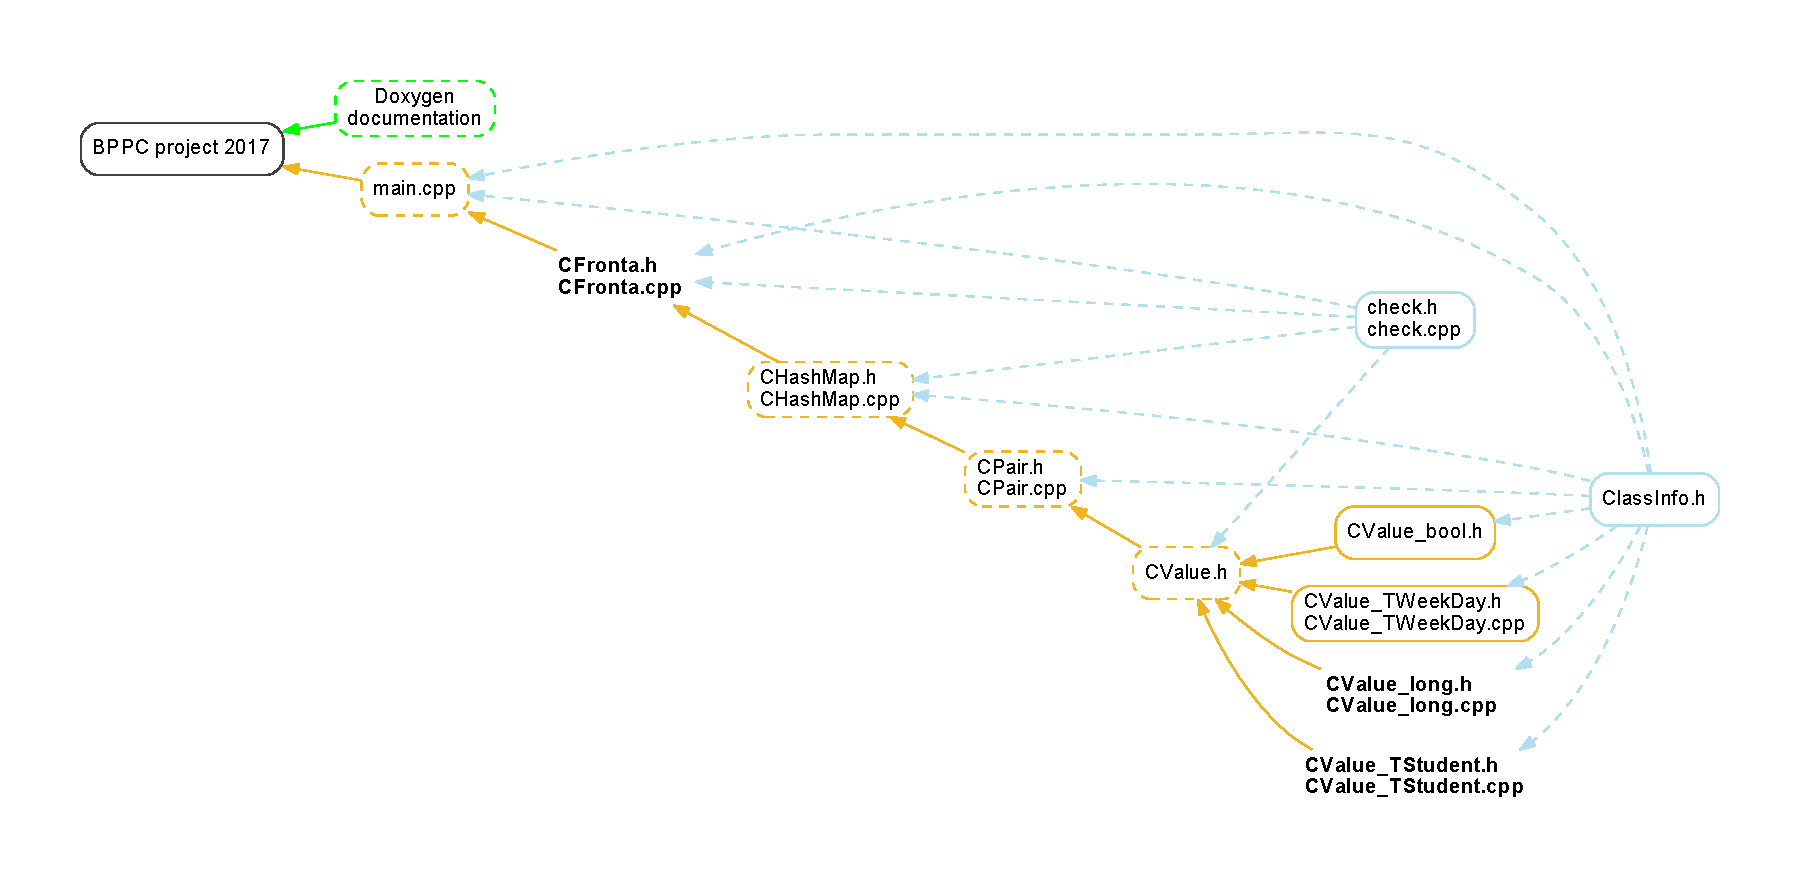
\includegraphics[width=\textwidth,height=\textheight/2,keepaspectratio=true]{dot_project_hierarchy}
\doxyfigcaption{Obr.1 -\/ Nákres hierarchie souboru v projektu}
\end{DoxyImage}
~\newline
 Vlastní realizace třídy pro {\bfseries kontejner} bude rozdělena na hlavičkový a zdrojový soubor ({\bfseries \hyperlink{_c_fronta_8h}{C\+Fronta.\+h}}, {\bfseries \hyperlink{_c_fronta_8cpp}{C\+Fronta.\+cpp}}). Další zdrojový soubor (\hyperlink{main_8cpp}{main.\+cpp}) bude reprezentovat program demonstrující vlastnosti a použití definované třídy {\bfseries \hyperlink{class_c_fronta}{C\+Fronta}}. Všechny zdrojové a hlavičkové soubory budou obsahovat úvodní poznámku o svém názvu, řešitelích...).

Demonstrační program bude realizován jako konzolová aplikace přeložitelná ve Visual C++ (prázdný projekt, přísnost (stupeň) překladu 3 na detekci chybových a varovných hlášení). Snažte se, aby demonstrační program byl napsán tak, aby při činnosti nevyžadoval zásahy obsluhy ani vstupní data z jiných speciálních souborů (s výjimkou operátoru pro standardní vstup). Demonstrační/testovací programu bude inicializovat proměnné (v něm definovanými daty nezadávanými uživatelem) a na jejich základě bude demonstrovat činnost třídy a dále zobrazovat data na konzolu, nebo ukládat výsledky do souboru. \hyperlink{doc}{Dokumentaci} výsledného projektu realizujte pomocí nástroje \href{http://www.doxygen.org}{\tt Doxygen}.

K tomuto odevzdávanému zadání nezapomeňte připsat úvod pro hlavičku (tj. jména řešitelů, název projektu, datum zadání ... budou součástí odevzdávaného souboru)

Na následujícím odkazu najdete \href{https://my.mindnode.com/s2Bbn2gFS8pHZFGcZJhRj4U7zmxx8ivygkoPCuZz}{\tt Myšlenkovou mapu k projektu}, kterou jsme tvořili během přednášky věnované projektu. Pro lepší orientaci uvádíme krátkou motivaci k pojmu třída na odkazu\+: \href{http://www.uamt.feec.vutbr.cz/~richter/vyuka/XPPC/bppc/cviceni/motivace_trida.html}{\tt Motivace třída}.

Pokud Vás trápí nastavení \href{https://en.wikipedia.org/wiki/Test-driven_development}{\tt Unit testů} ve V\+S2017 zkuste si projít \href{http://www.evernote.com/l/AElAKsn_ps1ONbQRPVcvgmGPXcK76B0P0qs/}{\tt tento postup}. ~\newline
~\newline
Poslední změna\+: \begin{DoxyParagraph}{Date}
2017-\/12-\/21
\end{DoxyParagraph}


\begin{DoxyParagraph}{Id}
\hyperlink{_introduction_8md}{Introduction.\+md} 2359 2017-\/12-\/21 19\+:09\+:33Z xlevri01 
\end{DoxyParagraph}

\chapter{Dokumentace projektu C\+Hash\+Map}
\label{doc}
\Hypertarget{doc}
\subsection*{Teoretický popis\+: Termín datový kontejner}

Termín kontejner představuje v oblasti návrhu datových struktur a algoritmů takový datový typ, který umožňuje za běhu programu sdružovat více prvků (stejného nebo i různého typu) do jedné společné složené datové struktury. Výhody spojené s používáním kontejneru lze najít například v jednoduchém předání všech prvků takového kontejneru do funkce pomocí jediného argumentu (typu kontejner), nebo pro předání více hodnot z funkce, kde návratovou hodnotou je opět jediná hodnota (typu kontejner). Hlavní výhodou je ovšem možnost provedení operace nad všemi prvky kontejneru pomocí zápisu jediného volání služby, kterou zajistí přímo daný kontejner v rámci svého A\+PI. Mezi takové služby může patřit dealokace paměti všech prvků v kontejneru, vytisknutí všech prvků v kontejneru a další operace spojené se správou prvků v kontejneru. Prvky vkládané do Vašeho budoucího datového kontejneru budou právě instance třídy {\ttfamily C\+Value}. Ale i na samotnou třídu {\ttfamily C\+Value} lze pohlížet jako na primitivní kontejner mající jedinou hodnotu.

\subsubsection*{Třída C\+Value}

Třída {\ttfamily C\+Value} obsahuje prvek (nebo prvky) mající hodnotu kterou jako třída zapouzdřuje ({\ttfamily bool}, {\ttfamily T\+Week\+Day}, {\bfseries long}, {\bfseries T\+Student}) {\itshape Nahraďte tučně označenou část zadanými typy!}

Úlohou třídy {\ttfamily C\+Value} je v definici mít složku {\ttfamily i\+Value}, jenž představuje užitečná data, která bude každý prvek seznamu obsahovat. Dále je třeba vhodně upravit (případně doplnit) metody určené pro konstrukci a likvidaci prvku tak, aby bylo možné nový prvek efektivně konstruovat a využívat. Třída {\ttfamily C\+Value} je navíc správcem své vlastní hodnoty {\ttfamily i\+Value} a proto definuje základní metody pro zjištění, nastavení této hodnoty a zároveň zajišťuje pro nadřazené vyšší části programu metody pro porovnání dvou prvků {\ttfamily C\+Value} dle této hodnoty, čímž izoluje nadřazené části od nutnosti znát konkrétní datový typ složky {\ttfamily i\+Value}.

\subsubsection*{Jmenné prostory C\+Value\+\_\+xxxx (\hyperlink{class_c_value__bool_1_1_c_value}{C\+Value\+\_\+bool\+::\+C\+Value}, \hyperlink{class_c_value___t_week_day_1_1_c_value}{C\+Value\+\_\+\+T\+Week\+Day\+::\+C\+Value})}

Návrh programu i Vaše zadání požaduje nezávislost na vnitřní implementaci třídy {\ttfamily C\+Value} (konkrétním datovém typu složky {\ttfamily i\+Value}). Návrh navíc umožňuje, aby uživatel mohl odkomentováním řádku přepínat mezi vnitřními implementacemi {\ttfamily C\+Value}. Tento mechanismus je zajištěn pomocí definice každé z variant {\ttfamily C\+Value} ve vlastním jmenném prostoru {\ttfamily C\+Value\+\_\+\+N\+A\+Z\+E\+V\+\_\+\+T\+Y\+PU}. Díky této skutečnosti může existovat v programu několik stejně pojmenovaných tříd {\ttfamily C\+Value}, neboť názvy existují ve svém vlastním oboru viditelnosti (jmenném prostoru).

Volba dané varianty {\ttfamily C\+Value} je potom prováděna v souboru \hyperlink{_c_value_8h}{C\+Value.\+h}, odkomentovaním toho řádku, který exportuje daný jmenný prostor do globálního prostoru jmen. 
\begin{DoxyCode}
\textcolor{keyword}{using namespace }\hyperlink{namespace_c_value__bool}{CValue\_bool};
\textcolor{comment}{//using namespace CValue\_TWeekDay;}
\textcolor{comment}{//using namespace CValue\_char;}
\textcolor{comment}{//using namespace CValue\_int;}
\textcolor{comment}{//using namespace CValue\_float;}
\textcolor{comment}{//using namespace CValue\_long\_double;}
\end{DoxyCode}


~\newline
\subsection*{Realizace dalších variant tříd C\+Value}

V současnosti projekt obsahuje tyto varianty tříd {\ttfamily C\+Value}, z nichž je každá definována ve svém jmenném prostoru\+: \begin{DoxyItemize}
\item \hyperlink{class_c_value__bool_1_1_c_value}{C\+Value\+\_\+bool\+::\+C\+Value} \item \hyperlink{class_c_value___t_week_day_1_1_c_value}{C\+Value\+\_\+\+T\+Week\+Day\+::\+C\+Value}\end{DoxyItemize}
{\bfseries Tyto dvě třídy jsou pevně zadány a je zakázáno modifikovat jejich zdrojové texty!} Pro každou další variantu {\ttfamily C\+Value} nadefinujte nový jmenný prostor {\ttfamily C\+Value\+\_\+\+N\+A\+Z\+E\+V\+\_\+\+T\+Y\+PU} a v něm implementujte novou variantu třídy {\ttfamily C\+Value}. \begin{DoxyNote}{Note}
Mechanismus by samozřejmě bylo možné realizovat i zcela automaticky (překladač sám dle potřeby programátora vygeneruje novou variantu třídy {\ttfamily C\+Value} pomocí definované šablony, případně bude umožnovat dynamickou identifikaci typu a tím umožní mít při běhu programu v jednom seznamu různé varianty prvků {\ttfamily C\+Value}. Obě tyto techniky ovšem svým rozsahem vybočují nad rámec výuky v tomto kurzu a proto jsme se rozhodli se jim v tomto projektu vyhnout.
\end{DoxyNote}
~\newline
\subsection*{Testovací hlavní program}

Hlavní program v souboru \hyperlink{main_8cpp}{main.\+cpp} představuje základní sadu testů, které ověřují správnou funkci libovolné varianty třídy {\ttfamily C\+Value}. Seznamte se s obsahem hlavního programu a trasujte si jednotlivá volání.

\subsubsection*{Testovací hodnoty}

Každá z implementací třídy {\ttfamily C\+Value} navíc obsahuje šest základních metod vracející hodnotu datového typu, který je vhodný pro vložení do složky {\ttfamily i\+Value}. Projděte si uvedené mechanismy a snažte se pochopit jejich vliv na nezávislost kódu hlavního programu.

Jedná se o tyto metody\+: \begin{DoxyItemize}
\item {\ttfamily Test\+Value0()} (např. \hyperlink{class_c_value__bool_1_1_c_value_a6a39f590a87bb4be8f707c032ca2b32b}{C\+Value\+\_\+bool\+::\+C\+Value\+::\+Test\+Value0()}) \item {\ttfamily Test\+String\+Value0()} (např. \hyperlink{class_c_value__bool_1_1_c_value_ae327d8276f5f4c75705c7413d5942ea0}{C\+Value\+\_\+bool\+::\+C\+Value\+::\+Test\+String\+Value0}) \item {\ttfamily Test\+Value1()} (např. \hyperlink{class_c_value__bool_1_1_c_value_a73b53a394f0b2ebeebeecad0610949b8}{C\+Value\+\_\+bool\+::\+C\+Value\+::\+Test\+Value1}) \item {\ttfamily Test\+String\+Value1()} (např. \hyperlink{class_c_value__bool_1_1_c_value_a2d82d7f212af01b330e3bc3514961a5a}{C\+Value\+\_\+bool\+::\+C\+Value\+::\+Test\+String\+Value1}) \item {\ttfamily Test\+Value\+Random()} (např. \hyperlink{class_c_value__bool_1_1_c_value_a5583585b33adfb3b27d9b49ad1a7cc3a}{C\+Value\+\_\+bool\+::\+C\+Value\+::\+Test\+Value\+Random}) \item {\ttfamily Test\+String\+Random()} (např. \hyperlink{class_c_value__bool_1_1_c_value_a84d39c7918bfb7876640a8b64e2e8c95}{C\+Value\+\_\+bool\+::\+C\+Value\+::\+Test\+String\+Value\+Random})\end{DoxyItemize}
\subsubsection*{Další kontrolní vlastnosti prvku}

Třída C\+Value obsahuje několik kontrolních a ladicích mechanismů, které budete jistě chtít využívat.

\begin{DoxyItemize}
\item Členskou proměnnou {\ttfamily i\+Instance} typu {\ttfamily Class\+Info} obsahující počítadlo vzniklých instancí (viz dále). \item Pokud budete v metodách třídy C\+Value dynamicky alokovat pamět nezapomeňte na kontroly dealokace paměti pomocí knihovny check. \item Pokud je prováděn překlad v {\itshape Debug režimu} je při každém spuštění zajištěna identická inicializace generátoru náhodných čísel. Tím při každém krokování programu bude generován pro stejná vstupní data identický seznam (výsledný kontejner bude obsahovat prvky se stejnými hodnotami pro každé spuštění). Až si budete jisti, že program je funkční, zkuste přepnout překlad do {\itshape Release režimu} a ověřit správnou funkci celého kontejneru při různých počátečních podmínkách generátoru náhodných čísel.\end{DoxyItemize}
\subsubsection*{Třída Class\+Info}

Třída Class\+Info implementuje mechanismus automatického počítání vzniklých objektů a mechanismus jednoznačné identifikace Class\+Info$<$$>$\+::\+ID \char`\"{}\+I\+D\char`\"{} instancí za běhu programu. Tento mechanismus se Vám bude hodit při ladění programu. Všechny Vaše třídy by měly obsahovat datovou složku \hyperlink{class_c_value__bool_1_1_c_value_a5e9470a5efc80373b5cc943f25d1a803}{i\+Instance\+Info} třídy Class\+Info, čímž zajistíte Vašim třídám tyto ladicí vlastnosti. Samotná třída Class\+Info je definována jako šablona umožňující, vznik různých variant této třídy -\/ (generické programování resp. metaprogramování).

Mezi ladicí metody třídy Class\+Info patří\+: \begin{DoxyItemize}
\item Class\+Info$<$\+T$>$\+::\+Total() -\/ počítadlo vzniklých instancí třídy T \item Class\+Info$<$\+T$>$\+::\+Living() -\/ počítadlo v daném okamžiku existujících instancí třídy T \item Class\+Info$<$\+T$>$\+::\+I\+D() resp. \hyperlink{class_c_value__bool_1_1_c_value_a028335ed71781b92b96dfb51e1118eda}{C\+Value\+:\+:ID()} -\/ unikátní číselné označení dané instance\end{DoxyItemize}
\begin{DoxyAttention}{Attention}
Projděte si všechny uvedené kontrolní i ladicí mechanismy, snažte se pochopit jejich smysl a využití při trasování programu. Získané vědomosti se Vám budou rozhodně hodit, například když se nějaká část Vašeho programu začne chovat \char`\"{}podezřele\char`\"{} či přímo \char`\"{}nepřátelsky\char`\"{}.
\end{DoxyAttention}
\begin{DoxyNote}{Note}
Hodně štěstí při realizaci Vašeho projektu. Nebojte se, ono to půjde. Hlavně {\itshape nepropadejte panice!} ;-\/)
\end{DoxyNote}
Pety.

\begin{DoxyParagraph}{Id}
\hyperlink{_documentation_8md}{Documentation.\+md} 1 2017-\/11-\/06 09\+:45\+:38Z petyovsky 
\end{DoxyParagraph}

\chapter{Todo List}
\label{todo}
\Hypertarget{todo}

\begin{DoxyRefList}
\item[\label{todo__todo000001}%
\Hypertarget{todo__todo000001}%
page \hyperlink{index}{Úvod a zadání} ]V následujících třech částech ponechejte v seznamu vždy pouze ty položky, které odpovídají Vašemu zadání projektu.

Místo všech názvů {\bfseries  {\ttfamily \hyperlink{class_c_container}{C\+Container}}} uveďte název kontejneru zvoleného v části zadání číslo 3

Od tohoto místa dále (včetně obrázku) nahraďte tučně zapsané texty vhodnou modifikací pro Vaše zadání (značky pro zvýraznění bold neodstraňujte). Nezvýrazněný text nemažte -\/ jedná se o povinné body zadání!!! Dále viz úvodní poznámky.

testy??? 14. Pro každou implementovanou metodu navrhněte alespoň 3 case testy. 
\end{DoxyRefList}
\chapter{Namespace Index}
\section{Namespace List}
Here is a list of all namespaces with brief descriptions\+:\begin{DoxyCompactList}
\item\contentsline{section}{\hyperlink{namespace_c_value__bool}{C\+Value\+\_\+bool} \\*Namespace for encapsulating of {\ttfamily bool} variant of \hyperlink{class_c_value__bool_1_1_c_value}{C\+Value} class }{\pageref{namespace_c_value__bool}}{}
\item\contentsline{section}{\hyperlink{namespace_c_value__long}{C\+Value\+\_\+long} \\*Namespace for encapsulating of {\ttfamily long} variant of \hyperlink{class_c_value__long_1_1_c_value}{C\+Value} class }{\pageref{namespace_c_value__long}}{}
\item\contentsline{section}{\hyperlink{namespace_c_value___t_student}{C\+Value\+\_\+\+T\+Student} \\*Namespace for encapsulating of {\ttfamily \hyperlink{struct_c_value___t_student_1_1_t_student}{T\+Student}} variant of \hyperlink{class_c_value___t_student_1_1_c_value}{C\+Value} class }{\pageref{namespace_c_value___t_student}}{}
\item\contentsline{section}{\hyperlink{namespace_c_value___t_week_day}{C\+Value\+\_\+\+T\+Week\+Day} \\*Namespace for encapsulating of {\ttfamily T\+Week\+Day} variant of \hyperlink{class_c_value___t_week_day_1_1_c_value}{C\+Value} class }{\pageref{namespace_c_value___t_week_day}}{}
\end{DoxyCompactList}

\chapter{Class Index}
\section{Class List}
Here are the classes, structs, unions and interfaces with brief descriptions\+:\begin{DoxyCompactList}
\item\contentsline{section}{\hyperlink{class_c_hash_map_1_1_c_forward_iterator}{C\+Hash\+Map\+::\+C\+Forward\+Iterator} \\*\hyperlink{class_c_hash_map_1_1_c_forward_iterator}{C\+Forward\+Iterator} class definition }{\pageref{class_c_hash_map_1_1_c_forward_iterator}}{}
\item\contentsline{section}{\hyperlink{class_c_hash_map}{C\+Hash\+Map} \\*\hyperlink{class_c_hash_map}{C\+Hash\+Map} class definition }{\pageref{class_c_hash_map}}{}
\item\contentsline{section}{\hyperlink{class_c_pair}{C\+Pair} \\*\hyperlink{class_c_pair}{C\+Pair} class (key and value) }{\pageref{class_c_pair}}{}
\item\contentsline{section}{\hyperlink{class_c_value__bool_1_1_c_value}{C\+Value\+\_\+bool\+::\+C\+Value} \\*\hyperlink{class_c_value__bool_1_1_c_value}{C\+Value} class ({\ttfamily bool} variant) }{\pageref{class_c_value__bool_1_1_c_value}}{}
\item\contentsline{section}{\hyperlink{class_c_value___t_student_1_1_c_value}{C\+Value\+\_\+\+T\+Student\+::\+C\+Value} \\*\hyperlink{class_c_value___t_student_1_1_c_value}{C\+Value} class ({\ttfamily \hyperlink{struct_c_value___t_student_1_1_t_student}{T\+Student}} variant) }{\pageref{class_c_value___t_student_1_1_c_value}}{}
\item\contentsline{section}{\hyperlink{class_c_value__long_1_1_c_value}{C\+Value\+\_\+long\+::\+C\+Value} \\*\hyperlink{class_c_value__long_1_1_c_value}{C\+Value} class ({\ttfamily long} variant) }{\pageref{class_c_value__long_1_1_c_value}}{}
\item\contentsline{section}{\hyperlink{class_c_value___t_week_day_1_1_c_value}{C\+Value\+\_\+\+T\+Week\+Day\+::\+C\+Value} \\*\hyperlink{class_c_value___t_week_day_1_1_c_value}{C\+Value} class ({\ttfamily T\+Week\+Day} variant) }{\pageref{class_c_value___t_week_day_1_1_c_value}}{}
\item\contentsline{section}{\hyperlink{struct_c_hash_map_1_1_t_bucket}{C\+Hash\+Map\+::\+T\+Bucket} \\*\hyperlink{struct_c_hash_map_1_1_t_bucket}{T\+Bucket} structure definition }{\pageref{struct_c_hash_map_1_1_t_bucket}}{}
\item\contentsline{section}{\hyperlink{struct_c_hash_map_1_1_t_item}{C\+Hash\+Map\+::\+T\+Item} \\*\hyperlink{struct_c_hash_map_1_1_t_item}{T\+Item} structure definiton }{\pageref{struct_c_hash_map_1_1_t_item}}{}
\item\contentsline{section}{\hyperlink{struct_c_value___t_student_1_1_t_student}{C\+Value\+\_\+\+T\+Student\+::\+T\+Student} \\*Basic definition of struct type for representing day of week }{\pageref{struct_c_value___t_student_1_1_t_student}}{}
\end{DoxyCompactList}

\chapter{File Index}
\section{File List}
Here is a list of all files with brief descriptions\+:\begin{DoxyCompactList}
\item\contentsline{section}{\hyperlink{_c_container_8cpp}{C\+Container.\+cpp} \\*\hyperlink{class_c_container}{C\+Container} class implementation }{\pageref{_c_container_8cpp}}{}
\item\contentsline{section}{\hyperlink{_c_container_8h}{C\+Container.\+h} \\*\hyperlink{class_c_container}{C\+Container} class header }{\pageref{_c_container_8h}}{}
\item\contentsline{section}{\hyperlink{_c_fronta_8cpp}{C\+Fronta.\+cpp} }{\pageref{_c_fronta_8cpp}}{}
\item\contentsline{section}{\hyperlink{_c_fronta_8h}{C\+Fronta.\+h} \\*\hyperlink{class_c_fronta}{C\+Fronta} class header }{\pageref{_c_fronta_8h}}{}
\item\contentsline{section}{\hyperlink{_c_hash_map_8cpp}{C\+Hash\+Map.\+cpp} \\*\hyperlink{class_c_hash_map}{C\+Hash\+Map} class implementation }{\pageref{_c_hash_map_8cpp}}{}
\item\contentsline{section}{\hyperlink{_c_hash_map_8h}{C\+Hash\+Map.\+h} \\*\hyperlink{class_c_hash_map}{C\+Hash\+Map} class header }{\pageref{_c_hash_map_8h}}{}
\item\contentsline{section}{\hyperlink{_c_pair_8cpp}{C\+Pair.\+cpp} \\*\hyperlink{class_c_pair}{C\+Pair} class implementation }{\pageref{_c_pair_8cpp}}{}
\item\contentsline{section}{\hyperlink{_c_pair_8h}{C\+Pair.\+h} \\*\hyperlink{class_c_pair}{C\+Pair} class header }{\pageref{_c_pair_8h}}{}
\item\contentsline{section}{\hyperlink{_c_value_8h}{C\+Value.\+h} \\*General header for C\+Value }{\pageref{_c_value_8h}}{}
\item\contentsline{section}{\hyperlink{_c_value__bool_8h}{C\+Value\+\_\+bool.\+h} \\*\hyperlink{namespace_c_value__bool}{C\+Value\+\_\+bool} class header }{\pageref{_c_value__bool_8h}}{}
\item\contentsline{section}{\hyperlink{_c_value__long_8h}{C\+Value\+\_\+long.\+h} \\*\hyperlink{namespace_c_value__long}{C\+Value\+\_\+long} class header }{\pageref{_c_value__long_8h}}{}
\item\contentsline{section}{\hyperlink{_c_value___t_student_8cpp}{C\+Value\+\_\+\+T\+Student.\+cpp} \\*\hyperlink{namespace_c_value___t_student}{C\+Value\+\_\+\+T\+Student} class source }{\pageref{_c_value___t_student_8cpp}}{}
\item\contentsline{section}{\hyperlink{_c_value___t_student_8h}{C\+Value\+\_\+\+T\+Student.\+h} \\*\hyperlink{namespace_c_value___t_student}{C\+Value\+\_\+\+T\+Student} class header }{\pageref{_c_value___t_student_8h}}{}
\item\contentsline{section}{\hyperlink{_c_value___t_week_day_8cpp}{C\+Value\+\_\+\+T\+Week\+Day.\+cpp} \\*\hyperlink{namespace_c_value___t_week_day}{C\+Value\+\_\+\+T\+Week\+Day} class source }{\pageref{_c_value___t_week_day_8cpp}}{}
\item\contentsline{section}{\hyperlink{_c_value___t_week_day_8h}{C\+Value\+\_\+\+T\+Week\+Day.\+h} \\*\hyperlink{namespace_c_value___t_week_day}{C\+Value\+\_\+\+T\+Week\+Day} class header }{\pageref{_c_value___t_week_day_8h}}{}
\item\contentsline{section}{\hyperlink{main_8cpp}{main.\+cpp} \\*Main source }{\pageref{main_8cpp}}{}
\end{DoxyCompactList}

\chapter{Namespace Documentation}
\hypertarget{namespace_c_value__bool}{}\section{C\+Value\+\_\+bool Namespace Reference}
\label{namespace_c_value__bool}\index{C\+Value\+\_\+bool@{C\+Value\+\_\+bool}}


Namespace for encapsulating of {\ttfamily bool} variant of \hyperlink{class_c_value__bool_1_1_c_value}{C\+Value} class.  


\subsection*{Classes}
\begin{DoxyCompactItemize}
\item 
class \hyperlink{class_c_value__bool_1_1_c_value}{C\+Value}
\begin{DoxyCompactList}\small\item\em \hyperlink{class_c_value__bool_1_1_c_value}{C\+Value} class ({\ttfamily bool} variant) \end{DoxyCompactList}\end{DoxyCompactItemize}


\subsection{Detailed Description}
Namespace for encapsulating of {\ttfamily bool} variant of \hyperlink{class_c_value__bool_1_1_c_value}{C\+Value} class. 

For selecting this variant of \hyperlink{class_c_value__bool_1_1_c_value}{C\+Value} class uncomment {\ttfamily using} {\ttfamily namespace} section in the \hyperlink{_c_value_8h}{C\+Value.\+h} 
\hypertarget{namespace_c_value__long}{}\section{C\+Value\+\_\+long Namespace Reference}
\label{namespace_c_value__long}\index{C\+Value\+\_\+long@{C\+Value\+\_\+long}}


Namespace for encapsulating of {\ttfamily long} variant of \hyperlink{class_c_value__long_1_1_c_value}{C\+Value} class.  


\subsection*{Classes}
\begin{DoxyCompactItemize}
\item 
class \hyperlink{class_c_value__long_1_1_c_value}{C\+Value}
\begin{DoxyCompactList}\small\item\em \hyperlink{class_c_value__long_1_1_c_value}{C\+Value} class ({\ttfamily long} variant) \end{DoxyCompactList}\end{DoxyCompactItemize}


\subsection{Detailed Description}
Namespace for encapsulating of {\ttfamily long} variant of \hyperlink{class_c_value__long_1_1_c_value}{C\+Value} class. 

For selecting this variant of \hyperlink{class_c_value__long_1_1_c_value}{C\+Value} class uncomment {\ttfamily using} {\ttfamily namespace} section in the \hyperlink{_c_value_8h}{C\+Value.\+h} 
\hypertarget{namespace_c_value___t_student}{}\section{C\+Value\+\_\+\+T\+Student Namespace Reference}
\label{namespace_c_value___t_student}\index{C\+Value\+\_\+\+T\+Student@{C\+Value\+\_\+\+T\+Student}}


Namespace for encapsulating of {\ttfamily \hyperlink{struct_c_value___t_student_1_1_t_student}{T\+Student}} variant of \hyperlink{class_c_value___t_student_1_1_c_value}{C\+Value} class.  


\subsection*{Classes}
\begin{DoxyCompactItemize}
\item 
class \hyperlink{class_c_value___t_student_1_1_c_value}{C\+Value}
\begin{DoxyCompactList}\small\item\em \hyperlink{class_c_value___t_student_1_1_c_value}{C\+Value} class ({\ttfamily \hyperlink{struct_c_value___t_student_1_1_t_student}{T\+Student}} variant) \end{DoxyCompactList}\item 
struct \hyperlink{struct_c_value___t_student_1_1_t_student}{T\+Student}
\begin{DoxyCompactList}\small\item\em Basic definition of struct type for representing \hyperlink{struct_c_value___t_student_1_1_t_student}{T\+Student}. \end{DoxyCompactList}\end{DoxyCompactItemize}
\subsection*{Functions}
\begin{DoxyCompactItemize}
\item 
std\+::ostream \& \hyperlink{namespace_c_value___t_student_a74d67e5f2ecbfee96605b87464c628ca}{operator$<$$<$} (std\+::ostream \&a\+O\+Stream, const \hyperlink{struct_c_value___t_student_1_1_t_student}{T\+Student} \&a\+Student)
\begin{DoxyCompactList}\small\item\em Output to the stream operator. ({\itshape serialization}) \end{DoxyCompactList}\item 
std\+::istream \& \hyperlink{namespace_c_value___t_student_a7cef4a5db96e988bb59a53168f90363f}{operator$>$$>$} (std\+::istream \&a\+I\+Stream, \hyperlink{struct_c_value___t_student_1_1_t_student}{T\+Student} \&a\+Student)
\begin{DoxyCompactList}\small\item\em Input from the stream operator. ({\itshape deserialization}) \end{DoxyCompactList}\end{DoxyCompactItemize}


\subsection{Detailed Description}
Namespace for encapsulating of {\ttfamily \hyperlink{struct_c_value___t_student_1_1_t_student}{T\+Student}} variant of \hyperlink{class_c_value___t_student_1_1_c_value}{C\+Value} class. 

For selecting this variant of \hyperlink{class_c_value___t_student_1_1_c_value}{C\+Value} class uncomment {\ttfamily using} {\ttfamily namespace} section in the \hyperlink{_c_value_8h}{C\+Value.\+h} 

\subsection{Function Documentation}
\mbox{\Hypertarget{namespace_c_value___t_student_a74d67e5f2ecbfee96605b87464c628ca}\label{namespace_c_value___t_student_a74d67e5f2ecbfee96605b87464c628ca}} 
\index{C\+Value\+\_\+\+T\+Student@{C\+Value\+\_\+\+T\+Student}!operator$<$$<$@{operator$<$$<$}}
\index{operator$<$$<$@{operator$<$$<$}!C\+Value\+\_\+\+T\+Student@{C\+Value\+\_\+\+T\+Student}}
\subsubsection{\texorpdfstring{operator$<$$<$()}{operator<<()}}
{\footnotesize\ttfamily std\+::ostream \& C\+Value\+\_\+\+T\+Student\+::operator$<$$<$ (\begin{DoxyParamCaption}\item[{std\+::ostream \&}]{a\+O\+Stream,  }\item[{const \hyperlink{struct_c_value___t_student_1_1_t_student}{T\+Student} \&}]{a\+Student }\end{DoxyParamCaption})}



Output to the stream operator. ({\itshape serialization}) 


\begin{DoxyParams}[1]{Parameters}
\mbox{\tt in}  & {\em a\+O\+Stream} & Output stream \\
\hline
\mbox{\tt in}  & {\em a\+Student} & Serialized instantion of \hyperlink{struct_c_value___t_student_1_1_t_student}{T\+Student} \\
\hline
\end{DoxyParams}
\begin{DoxyReturn}{Returns}
Return {\ttfamily std\+::ostream} with serialized a\+Student 
\end{DoxyReturn}


Definition at line 13 of file C\+Value\+\_\+\+T\+Student.\+cpp.

\mbox{\Hypertarget{namespace_c_value___t_student_a7cef4a5db96e988bb59a53168f90363f}\label{namespace_c_value___t_student_a7cef4a5db96e988bb59a53168f90363f}} 
\index{C\+Value\+\_\+\+T\+Student@{C\+Value\+\_\+\+T\+Student}!operator$>$$>$@{operator$>$$>$}}
\index{operator$>$$>$@{operator$>$$>$}!C\+Value\+\_\+\+T\+Student@{C\+Value\+\_\+\+T\+Student}}
\subsubsection{\texorpdfstring{operator$>$$>$()}{operator>>()}}
{\footnotesize\ttfamily std\+::istream \& C\+Value\+\_\+\+T\+Student\+::operator$>$$>$ (\begin{DoxyParamCaption}\item[{std\+::istream \&}]{a\+I\+Stream,  }\item[{\hyperlink{struct_c_value___t_student_1_1_t_student}{T\+Student} \&}]{a\+Student }\end{DoxyParamCaption})}



Input from the stream operator. ({\itshape deserialization}) 


\begin{DoxyParams}[1]{Parameters}
\mbox{\tt in}  & {\em a\+I\+Stream} & Input stream \\
\hline
\mbox{\tt out}  & {\em a\+Student} & Place for deserialized instantion of \hyperlink{struct_c_value___t_student_1_1_t_student}{T\+Student} \\
\hline
\end{DoxyParams}
\begin{DoxyReturn}{Returns}
Return rest of {\ttfamily std\+::istream} 
\end{DoxyReturn}


Definition at line 19 of file C\+Value\+\_\+\+T\+Student.\+cpp.


\hypertarget{namespace_c_value___t_week_day}{}\section{C\+Value\+\_\+\+T\+Week\+Day Namespace Reference}
\label{namespace_c_value___t_week_day}\index{C\+Value\+\_\+\+T\+Week\+Day@{C\+Value\+\_\+\+T\+Week\+Day}}


Namespace for encapsulating of {\ttfamily T\+Week\+Day} variant of \hyperlink{class_c_value___t_week_day_1_1_c_value}{C\+Value} class.  


\subsection*{Classes}
\begin{DoxyCompactItemize}
\item 
class \hyperlink{class_c_value___t_week_day_1_1_c_value}{C\+Value}
\begin{DoxyCompactList}\small\item\em \hyperlink{class_c_value___t_week_day_1_1_c_value}{C\+Value} class ({\ttfamily T\+Week\+Day} variant) \end{DoxyCompactList}\end{DoxyCompactItemize}
\subsection*{Enumerations}
\begin{DoxyCompactItemize}
\item 
enum \{ \hyperlink{namespace_c_value___t_week_day_ae2f386969b6b243f70cc768d81d87f37a82610dbf312a8592086eff40a38e1ff8}{K\+T\+Week\+Days\+Name\+Max\+Length} = 11
 \}
\item 
enum \hyperlink{namespace_c_value___t_week_day_a6412f204509f223b789fb5f1a61a6124}{T\+Week\+Day} \{ \newline
\hyperlink{namespace_c_value___t_week_day_a6412f204509f223b789fb5f1a61a6124a13c1447b2f5be5b292b403d71b5460b9}{E\+Monday} = 0, 
\hyperlink{namespace_c_value___t_week_day_a6412f204509f223b789fb5f1a61a6124ac54a40e76745b36a2315ffed4edbce80}{E\+Tuesday}, 
\hyperlink{namespace_c_value___t_week_day_a6412f204509f223b789fb5f1a61a6124ac611066963726ce53657cedaaaefc3d5}{E\+Wednesday}, 
\hyperlink{namespace_c_value___t_week_day_a6412f204509f223b789fb5f1a61a6124a7fb51985580d1ba92e55f2577a04b3b1}{E\+Thursday}, 
\newline
\hyperlink{namespace_c_value___t_week_day_a6412f204509f223b789fb5f1a61a6124a5d2ecb8bb6c29d8ecbfc5901ab383978}{E\+Friday}, 
\hyperlink{namespace_c_value___t_week_day_a6412f204509f223b789fb5f1a61a6124ab3e8b0a563537c9cd6ef20d06b486100}{E\+Saturday}, 
\hyperlink{namespace_c_value___t_week_day_a6412f204509f223b789fb5f1a61a6124ad4ed77e2d38772a8a5f77e9f87621117}{E\+Sunday}
 \}\begin{DoxyCompactList}\small\item\em Basic definition of enumeration type for representing day of week. \end{DoxyCompactList}
\item 
enum \{ \hyperlink{namespace_c_value___t_week_day_aafc13db7f1761bc02fc24499d9d30ef8aa662532b91895c243892c79eaafea534}{K\+T\+Week\+Days\+Count} = 7
 \}\begin{DoxyCompactList}\small\item\em Constant defining numbers of day in the week. \end{DoxyCompactList}
\end{DoxyCompactItemize}
\subsection*{Functions}
\begin{DoxyCompactItemize}
\item 
\hyperlink{namespace_c_value___t_week_day_a6412f204509f223b789fb5f1a61a6124}{T\+Week\+Day} \hyperlink{namespace_c_value___t_week_day_ae635bc6aae42ff925b25ce335390083b}{Check\+Range\+With\+Exception} (const unsigned a\+Day\+Num)
\begin{DoxyCompactList}\small\item\em Conversion and range checking function. Convert {\ttfamily unsigned} value to the T\+Week\+Day. \end{DoxyCompactList}\item 
const char $\ast$ \hyperlink{namespace_c_value___t_week_day_ad69753a29bce4084fa5dc888526b2bf2}{T\+Week\+String\+Name} (\hyperlink{namespace_c_value___t_week_day_a6412f204509f223b789fb5f1a61a6124}{T\+Week\+Day} a\+Week\+Day)
\begin{DoxyCompactList}\small\item\em Conversion Day number to the Day name. \end{DoxyCompactList}\item 
std\+::ostream \& \hyperlink{namespace_c_value___t_week_day_a0783ff307d102432c842a4d943b3d063}{operator$<$$<$} (std\+::ostream \&a\+O\+Stream, const \hyperlink{namespace_c_value___t_week_day_a6412f204509f223b789fb5f1a61a6124}{T\+Week\+Day} \&a\+Week\+Day)
\begin{DoxyCompactList}\small\item\em Output to the stream operator. ({\itshape serialization}) \end{DoxyCompactList}\item 
std\+::istream \& \hyperlink{namespace_c_value___t_week_day_ada60106206184e32b42cc05978db4d37}{operator$>$$>$} (std\+::istream \&a\+I\+Stream, \hyperlink{namespace_c_value___t_week_day_a6412f204509f223b789fb5f1a61a6124}{T\+Week\+Day} \&a\+Week\+Day)
\begin{DoxyCompactList}\small\item\em Input from the stream operator. ({\itshape deserialization}) \end{DoxyCompactList}\end{DoxyCompactItemize}
\subsection*{Variables}
\begin{DoxyCompactItemize}
\item 
static const char $\ast$const \hyperlink{namespace_c_value___t_week_day_a1c30aa5c20b662fe3dd12e7c26507d27}{K\+T\+Week\+Days\+Name} \mbox{[}\hyperlink{namespace_c_value___t_week_day_aafc13db7f1761bc02fc24499d9d30ef8aa662532b91895c243892c79eaafea534}{K\+T\+Week\+Days\+Count}\mbox{]}
\begin{DoxyCompactList}\small\item\em Day name definition. \end{DoxyCompactList}\end{DoxyCompactItemize}


\subsection{Detailed Description}
Namespace for encapsulating of {\ttfamily T\+Week\+Day} variant of \hyperlink{class_c_value___t_week_day_1_1_c_value}{C\+Value} class. 

For selecting this variant of \hyperlink{class_c_value___t_week_day_1_1_c_value}{C\+Value} class uncomment {\ttfamily using} {\ttfamily namespace} section in the \hyperlink{_c_value_8h}{C\+Value.\+h} 

\subsection{Enumeration Type Documentation}
\mbox{\Hypertarget{namespace_c_value___t_week_day_ae2f386969b6b243f70cc768d81d87f37}\label{namespace_c_value___t_week_day_ae2f386969b6b243f70cc768d81d87f37}} 
\subsubsection{\texorpdfstring{anonymous enum}{anonymous enum}}
{\footnotesize\ttfamily anonymous enum}

\begin{DoxyEnumFields}{Enumerator}
\raisebox{\heightof{T}}[0pt][0pt]{\index{K\+T\+Week\+Days\+Name\+Max\+Length@{K\+T\+Week\+Days\+Name\+Max\+Length}!C\+Value\+\_\+\+T\+Week\+Day@{C\+Value\+\_\+\+T\+Week\+Day}}\index{C\+Value\+\_\+\+T\+Week\+Day@{C\+Value\+\_\+\+T\+Week\+Day}!K\+T\+Week\+Days\+Name\+Max\+Length@{K\+T\+Week\+Days\+Name\+Max\+Length}}}\mbox{\Hypertarget{namespace_c_value___t_week_day_ae2f386969b6b243f70cc768d81d87f37a82610dbf312a8592086eff40a38e1ff8}\label{namespace_c_value___t_week_day_ae2f386969b6b243f70cc768d81d87f37a82610dbf312a8592086eff40a38e1ff8}} 
K\+T\+Week\+Days\+Name\+Max\+Length&\\
\hline

\end{DoxyEnumFields}


Definition at line 15 of file C\+Value\+\_\+\+T\+Week\+Day.\+cpp.

\mbox{\Hypertarget{namespace_c_value___t_week_day_aafc13db7f1761bc02fc24499d9d30ef8}\label{namespace_c_value___t_week_day_aafc13db7f1761bc02fc24499d9d30ef8}} 
\subsubsection{\texorpdfstring{anonymous enum}{anonymous enum}}
{\footnotesize\ttfamily anonymous enum}



Constant defining numbers of day in the week. 

\begin{DoxyEnumFields}{Enumerator}
\raisebox{\heightof{T}}[0pt][0pt]{\index{K\+T\+Week\+Days\+Count@{K\+T\+Week\+Days\+Count}!C\+Value\+\_\+\+T\+Week\+Day@{C\+Value\+\_\+\+T\+Week\+Day}}\index{C\+Value\+\_\+\+T\+Week\+Day@{C\+Value\+\_\+\+T\+Week\+Day}!K\+T\+Week\+Days\+Count@{K\+T\+Week\+Days\+Count}}}\mbox{\Hypertarget{namespace_c_value___t_week_day_aafc13db7f1761bc02fc24499d9d30ef8aa662532b91895c243892c79eaafea534}\label{namespace_c_value___t_week_day_aafc13db7f1761bc02fc24499d9d30ef8aa662532b91895c243892c79eaafea534}} 
K\+T\+Week\+Days\+Count&\\
\hline

\end{DoxyEnumFields}


Definition at line 31 of file C\+Value\+\_\+\+T\+Week\+Day.\+h.

\mbox{\Hypertarget{namespace_c_value___t_week_day_a6412f204509f223b789fb5f1a61a6124}\label{namespace_c_value___t_week_day_a6412f204509f223b789fb5f1a61a6124}} 
\index{C\+Value\+\_\+\+T\+Week\+Day@{C\+Value\+\_\+\+T\+Week\+Day}!T\+Week\+Day@{T\+Week\+Day}}
\index{T\+Week\+Day@{T\+Week\+Day}!C\+Value\+\_\+\+T\+Week\+Day@{C\+Value\+\_\+\+T\+Week\+Day}}
\subsubsection{\texorpdfstring{T\+Week\+Day}{TWeekDay}}
{\footnotesize\ttfamily enum \hyperlink{namespace_c_value___t_week_day_a6412f204509f223b789fb5f1a61a6124}{C\+Value\+\_\+\+T\+Week\+Day\+::\+T\+Week\+Day}}



Basic definition of enumeration type for representing day of week. 

\begin{DoxyEnumFields}{Enumerator}
\raisebox{\heightof{T}}[0pt][0pt]{\index{E\+Monday@{E\+Monday}!C\+Value\+\_\+\+T\+Week\+Day@{C\+Value\+\_\+\+T\+Week\+Day}}\index{C\+Value\+\_\+\+T\+Week\+Day@{C\+Value\+\_\+\+T\+Week\+Day}!E\+Monday@{E\+Monday}}}\mbox{\Hypertarget{namespace_c_value___t_week_day_a6412f204509f223b789fb5f1a61a6124a13c1447b2f5be5b292b403d71b5460b9}\label{namespace_c_value___t_week_day_a6412f204509f223b789fb5f1a61a6124a13c1447b2f5be5b292b403d71b5460b9}} 
E\+Monday&\\
\hline

\raisebox{\heightof{T}}[0pt][0pt]{\index{E\+Tuesday@{E\+Tuesday}!C\+Value\+\_\+\+T\+Week\+Day@{C\+Value\+\_\+\+T\+Week\+Day}}\index{C\+Value\+\_\+\+T\+Week\+Day@{C\+Value\+\_\+\+T\+Week\+Day}!E\+Tuesday@{E\+Tuesday}}}\mbox{\Hypertarget{namespace_c_value___t_week_day_a6412f204509f223b789fb5f1a61a6124ac54a40e76745b36a2315ffed4edbce80}\label{namespace_c_value___t_week_day_a6412f204509f223b789fb5f1a61a6124ac54a40e76745b36a2315ffed4edbce80}} 
E\+Tuesday&\\
\hline

\raisebox{\heightof{T}}[0pt][0pt]{\index{E\+Wednesday@{E\+Wednesday}!C\+Value\+\_\+\+T\+Week\+Day@{C\+Value\+\_\+\+T\+Week\+Day}}\index{C\+Value\+\_\+\+T\+Week\+Day@{C\+Value\+\_\+\+T\+Week\+Day}!E\+Wednesday@{E\+Wednesday}}}\mbox{\Hypertarget{namespace_c_value___t_week_day_a6412f204509f223b789fb5f1a61a6124ac611066963726ce53657cedaaaefc3d5}\label{namespace_c_value___t_week_day_a6412f204509f223b789fb5f1a61a6124ac611066963726ce53657cedaaaefc3d5}} 
E\+Wednesday&\\
\hline

\raisebox{\heightof{T}}[0pt][0pt]{\index{E\+Thursday@{E\+Thursday}!C\+Value\+\_\+\+T\+Week\+Day@{C\+Value\+\_\+\+T\+Week\+Day}}\index{C\+Value\+\_\+\+T\+Week\+Day@{C\+Value\+\_\+\+T\+Week\+Day}!E\+Thursday@{E\+Thursday}}}\mbox{\Hypertarget{namespace_c_value___t_week_day_a6412f204509f223b789fb5f1a61a6124a7fb51985580d1ba92e55f2577a04b3b1}\label{namespace_c_value___t_week_day_a6412f204509f223b789fb5f1a61a6124a7fb51985580d1ba92e55f2577a04b3b1}} 
E\+Thursday&\\
\hline

\raisebox{\heightof{T}}[0pt][0pt]{\index{E\+Friday@{E\+Friday}!C\+Value\+\_\+\+T\+Week\+Day@{C\+Value\+\_\+\+T\+Week\+Day}}\index{C\+Value\+\_\+\+T\+Week\+Day@{C\+Value\+\_\+\+T\+Week\+Day}!E\+Friday@{E\+Friday}}}\mbox{\Hypertarget{namespace_c_value___t_week_day_a6412f204509f223b789fb5f1a61a6124a5d2ecb8bb6c29d8ecbfc5901ab383978}\label{namespace_c_value___t_week_day_a6412f204509f223b789fb5f1a61a6124a5d2ecb8bb6c29d8ecbfc5901ab383978}} 
E\+Friday&\\
\hline

\raisebox{\heightof{T}}[0pt][0pt]{\index{E\+Saturday@{E\+Saturday}!C\+Value\+\_\+\+T\+Week\+Day@{C\+Value\+\_\+\+T\+Week\+Day}}\index{C\+Value\+\_\+\+T\+Week\+Day@{C\+Value\+\_\+\+T\+Week\+Day}!E\+Saturday@{E\+Saturday}}}\mbox{\Hypertarget{namespace_c_value___t_week_day_a6412f204509f223b789fb5f1a61a6124ab3e8b0a563537c9cd6ef20d06b486100}\label{namespace_c_value___t_week_day_a6412f204509f223b789fb5f1a61a6124ab3e8b0a563537c9cd6ef20d06b486100}} 
E\+Saturday&\\
\hline

\raisebox{\heightof{T}}[0pt][0pt]{\index{E\+Sunday@{E\+Sunday}!C\+Value\+\_\+\+T\+Week\+Day@{C\+Value\+\_\+\+T\+Week\+Day}}\index{C\+Value\+\_\+\+T\+Week\+Day@{C\+Value\+\_\+\+T\+Week\+Day}!E\+Sunday@{E\+Sunday}}}\mbox{\Hypertarget{namespace_c_value___t_week_day_a6412f204509f223b789fb5f1a61a6124ad4ed77e2d38772a8a5f77e9f87621117}\label{namespace_c_value___t_week_day_a6412f204509f223b789fb5f1a61a6124ad4ed77e2d38772a8a5f77e9f87621117}} 
E\+Sunday&\\
\hline

\end{DoxyEnumFields}


Definition at line 26 of file C\+Value\+\_\+\+T\+Week\+Day.\+h.



\subsection{Function Documentation}
\mbox{\Hypertarget{namespace_c_value___t_week_day_ae635bc6aae42ff925b25ce335390083b}\label{namespace_c_value___t_week_day_ae635bc6aae42ff925b25ce335390083b}} 
\index{C\+Value\+\_\+\+T\+Week\+Day@{C\+Value\+\_\+\+T\+Week\+Day}!Check\+Range\+With\+Exception@{Check\+Range\+With\+Exception}}
\index{Check\+Range\+With\+Exception@{Check\+Range\+With\+Exception}!C\+Value\+\_\+\+T\+Week\+Day@{C\+Value\+\_\+\+T\+Week\+Day}}
\subsubsection{\texorpdfstring{Check\+Range\+With\+Exception()}{CheckRangeWithException()}}
{\footnotesize\ttfamily \hyperlink{namespace_c_value___t_week_day_a6412f204509f223b789fb5f1a61a6124}{T\+Week\+Day} C\+Value\+\_\+\+T\+Week\+Day\+::\+Check\+Range\+With\+Exception (\begin{DoxyParamCaption}\item[{const unsigned}]{a\+Day\+Num }\end{DoxyParamCaption})}



Conversion and range checking function. Convert {\ttfamily unsigned} value to the T\+Week\+Day. 


\begin{DoxyParams}[1]{Parameters}
\mbox{\tt in}  & {\em a\+Day\+Num} & Number of day \\
\hline
\end{DoxyParams}
\begin{DoxyReturn}{Returns}
Return T\+Week\+Day value 
\end{DoxyReturn}
\begin{DoxyAttention}{Attention}
Method generate {\ttfamily std\+::range\+\_\+error} exception if argument {\itshape a\+Day\+Num} is out of numbers of the day 
\end{DoxyAttention}


Definition at line 19 of file C\+Value\+\_\+\+T\+Week\+Day.\+cpp.

\mbox{\Hypertarget{namespace_c_value___t_week_day_a0783ff307d102432c842a4d943b3d063}\label{namespace_c_value___t_week_day_a0783ff307d102432c842a4d943b3d063}} 
\index{C\+Value\+\_\+\+T\+Week\+Day@{C\+Value\+\_\+\+T\+Week\+Day}!operator$<$$<$@{operator$<$$<$}}
\index{operator$<$$<$@{operator$<$$<$}!C\+Value\+\_\+\+T\+Week\+Day@{C\+Value\+\_\+\+T\+Week\+Day}}
\subsubsection{\texorpdfstring{operator$<$$<$()}{operator<<()}}
{\footnotesize\ttfamily std\+::ostream \& C\+Value\+\_\+\+T\+Week\+Day\+::operator$<$$<$ (\begin{DoxyParamCaption}\item[{std\+::ostream \&}]{a\+O\+Stream,  }\item[{const \hyperlink{namespace_c_value___t_week_day_a6412f204509f223b789fb5f1a61a6124}{T\+Week\+Day} \&}]{a\+Week\+Day }\end{DoxyParamCaption})}



Output to the stream operator. ({\itshape serialization}) 


\begin{DoxyParams}[1]{Parameters}
\mbox{\tt in}  & {\em a\+O\+Stream} & Output stream \\
\hline
\mbox{\tt in}  & {\em a\+Week\+Day} & Serialized instantion of T\+Week\+Day \\
\hline
\end{DoxyParams}
\begin{DoxyReturn}{Returns}
Return {\ttfamily std\+::ostream} with serialized a\+Week\+Day 
\end{DoxyReturn}


Definition at line 32 of file C\+Value\+\_\+\+T\+Week\+Day.\+cpp.

\mbox{\Hypertarget{namespace_c_value___t_week_day_ada60106206184e32b42cc05978db4d37}\label{namespace_c_value___t_week_day_ada60106206184e32b42cc05978db4d37}} 
\index{C\+Value\+\_\+\+T\+Week\+Day@{C\+Value\+\_\+\+T\+Week\+Day}!operator$>$$>$@{operator$>$$>$}}
\index{operator$>$$>$@{operator$>$$>$}!C\+Value\+\_\+\+T\+Week\+Day@{C\+Value\+\_\+\+T\+Week\+Day}}
\subsubsection{\texorpdfstring{operator$>$$>$()}{operator>>()}}
{\footnotesize\ttfamily std\+::istream \& C\+Value\+\_\+\+T\+Week\+Day\+::operator$>$$>$ (\begin{DoxyParamCaption}\item[{std\+::istream \&}]{a\+I\+Stream,  }\item[{\hyperlink{namespace_c_value___t_week_day_a6412f204509f223b789fb5f1a61a6124}{T\+Week\+Day} \&}]{a\+Week\+Day }\end{DoxyParamCaption})}



Input from the stream operator. ({\itshape deserialization}) 


\begin{DoxyParams}[1]{Parameters}
\mbox{\tt in}  & {\em a\+I\+Stream} & Input stream \\
\hline
\mbox{\tt out}  & {\em a\+Week\+Day} & Place for deserialized instantion of T\+Week\+Day \\
\hline
\end{DoxyParams}
\begin{DoxyReturn}{Returns}
Return rest of {\ttfamily std\+::istream} 
\end{DoxyReturn}
\begin{DoxyAttention}{Attention}
Method generate {\ttfamily std\+::range\+\_\+error} exception if stream doesn\textquotesingle{}t contains correct name of the day 

Method generate {\ttfamily std\+::runtime\+\_\+error} exception if stream isn\textquotesingle{}t in good state 
\end{DoxyAttention}


Definition at line 38 of file C\+Value\+\_\+\+T\+Week\+Day.\+cpp.

\mbox{\Hypertarget{namespace_c_value___t_week_day_ad69753a29bce4084fa5dc888526b2bf2}\label{namespace_c_value___t_week_day_ad69753a29bce4084fa5dc888526b2bf2}} 
\index{C\+Value\+\_\+\+T\+Week\+Day@{C\+Value\+\_\+\+T\+Week\+Day}!T\+Week\+String\+Name@{T\+Week\+String\+Name}}
\index{T\+Week\+String\+Name@{T\+Week\+String\+Name}!C\+Value\+\_\+\+T\+Week\+Day@{C\+Value\+\_\+\+T\+Week\+Day}}
\subsubsection{\texorpdfstring{T\+Week\+String\+Name()}{TWeekStringName()}}
{\footnotesize\ttfamily const char $\ast$ C\+Value\+\_\+\+T\+Week\+Day\+::\+T\+Week\+String\+Name (\begin{DoxyParamCaption}\item[{\hyperlink{namespace_c_value___t_week_day_a6412f204509f223b789fb5f1a61a6124}{T\+Week\+Day}}]{a\+Week\+Day }\end{DoxyParamCaption})}



Conversion Day number to the Day name. 


\begin{DoxyParams}[1]{Parameters}
\mbox{\tt in}  & {\em a\+Week\+Day} & Day enumeration \\
\hline
\end{DoxyParams}
\begin{DoxyReturn}{Returns}
Return Day name 
\end{DoxyReturn}


Definition at line 29 of file C\+Value\+\_\+\+T\+Week\+Day.\+cpp.



\subsection{Variable Documentation}
\mbox{\Hypertarget{namespace_c_value___t_week_day_a1c30aa5c20b662fe3dd12e7c26507d27}\label{namespace_c_value___t_week_day_a1c30aa5c20b662fe3dd12e7c26507d27}} 
\index{C\+Value\+\_\+\+T\+Week\+Day@{C\+Value\+\_\+\+T\+Week\+Day}!K\+T\+Week\+Days\+Name@{K\+T\+Week\+Days\+Name}}
\index{K\+T\+Week\+Days\+Name@{K\+T\+Week\+Days\+Name}!C\+Value\+\_\+\+T\+Week\+Day@{C\+Value\+\_\+\+T\+Week\+Day}}
\subsubsection{\texorpdfstring{K\+T\+Week\+Days\+Name}{KTWeekDaysName}}
{\footnotesize\ttfamily const char$\ast$ const C\+Value\+\_\+\+T\+Week\+Day\+::\+K\+T\+Week\+Days\+Name\mbox{[}\hyperlink{namespace_c_value___t_week_day_aafc13db7f1761bc02fc24499d9d30ef8aa662532b91895c243892c79eaafea534}{K\+T\+Week\+Days\+Count}\mbox{]}\hspace{0.3cm}{\ttfamily [static]}}

{\bfseries Initial value\+:}
\begin{DoxyCode}
=
                \{ \textcolor{stringliteral}{"(Monday)"}, \textcolor{stringliteral}{"(Tuesday)"}, \textcolor{stringliteral}{"(Wednesday)"}, \textcolor{stringliteral}{"(Thursday)"}, \textcolor{stringliteral}{"(Friday)"}, \textcolor{stringliteral}{"(Saturday)"}, \textcolor{stringliteral}{"(Sunday)
      "} \}
\end{DoxyCode}


Day name definition. 



Definition at line 16 of file C\+Value\+\_\+\+T\+Week\+Day.\+cpp.


\chapter{Class Documentation}
\hypertarget{class_c_hash_map_1_1_c_forward_iterator}{}\section{C\+Hash\+Map\+:\+:C\+Forward\+Iterator Class Reference}
\label{class_c_hash_map_1_1_c_forward_iterator}\index{C\+Hash\+Map\+::\+C\+Forward\+Iterator@{C\+Hash\+Map\+::\+C\+Forward\+Iterator}}


\hyperlink{class_c_hash_map_1_1_c_forward_iterator}{C\+Forward\+Iterator} class definition.  




{\ttfamily \#include $<$C\+Hash\+Map.\+h$>$}



Collaboration diagram for C\+Hash\+Map\+:\+:C\+Forward\+Iterator\+:
\nopagebreak
\begin{figure}[H]
\begin{center}
\leavevmode
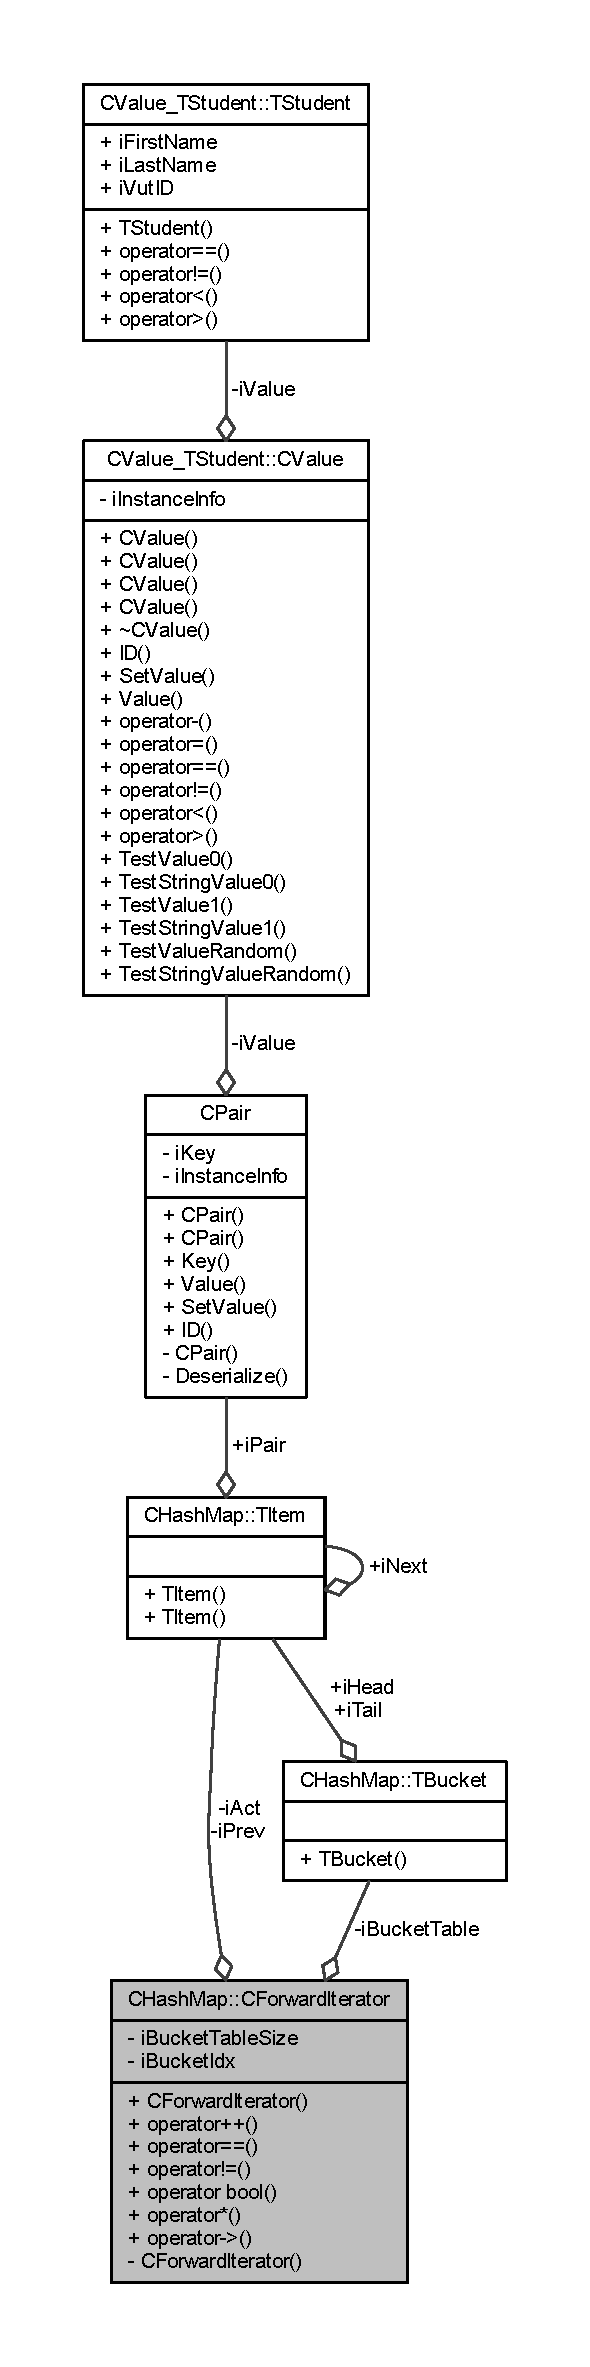
\includegraphics[height=550pt]{class_c_hash_map_1_1_c_forward_iterator__coll__graph}
\end{center}
\end{figure}
\subsection*{Public Member Functions}
\begin{DoxyCompactItemize}
\item 
\hyperlink{class_c_hash_map_1_1_c_forward_iterator_a2099500f60cfbe8c8c4d801d90010085}{C\+Forward\+Iterator} ()
\begin{DoxyCompactList}\small\item\em Implicit c\textquotesingle{}tor of \hyperlink{class_c_hash_map_1_1_c_forward_iterator}{C\+Forward\+Iterator} instance. \end{DoxyCompactList}\item 
\hyperlink{class_c_hash_map_1_1_c_forward_iterator}{C\+Forward\+Iterator} \& \hyperlink{class_c_hash_map_1_1_c_forward_iterator_a91997b9621fd4f421b349a2395100184}{operator++} ()
\begin{DoxyCompactList}\small\item\em Iterator pre-\/increment operator. \end{DoxyCompactList}\item 
bool \hyperlink{class_c_hash_map_1_1_c_forward_iterator_a251df2cf775a888851a03ac68015f705}{operator==} (const \hyperlink{class_c_hash_map_1_1_c_forward_iterator}{C\+Forward\+Iterator} \&a\+Iter) const
\begin{DoxyCompactList}\small\item\em Iterators equal to comparison operator. \end{DoxyCompactList}\item 
bool \hyperlink{class_c_hash_map_1_1_c_forward_iterator_a44785d54dad6b20115e28cd9df5ac0b9}{operator!=} (const \hyperlink{class_c_hash_map_1_1_c_forward_iterator}{C\+Forward\+Iterator} \&a\+Iter) const
\begin{DoxyCompactList}\small\item\em Iterators not equal to comparison operator. \end{DoxyCompactList}\item 
\hyperlink{class_c_hash_map_1_1_c_forward_iterator_a0afdbdba3d254474cd8c40a96f0469b8}{operator bool} () const
\begin{DoxyCompactList}\small\item\em Iterator conversion operator. \end{DoxyCompactList}\item 
\hyperlink{class_c_pair}{C\+Pair} \& \hyperlink{class_c_hash_map_1_1_c_forward_iterator_a7f44403bd74fc55f0263b56cf15fc64b}{operator$\ast$} () const
\begin{DoxyCompactList}\small\item\em Iterator dereferencing (indirection) operator. \end{DoxyCompactList}\item 
\hyperlink{class_c_pair}{C\+Pair} $\ast$ \hyperlink{class_c_hash_map_1_1_c_forward_iterator_a65fde4bd503e69c29b15688cd8c21eaf}{operator-\/$>$} () const
\begin{DoxyCompactList}\small\item\em Iterator member of pointer operator. \end{DoxyCompactList}\end{DoxyCompactItemize}
\subsection*{Private Member Functions}
\begin{DoxyCompactItemize}
\item 
\hyperlink{class_c_hash_map_1_1_c_forward_iterator_a1e27b10a503e0bdddce6bacdd91d16e3}{C\+Forward\+Iterator} (\hyperlink{struct_c_hash_map_1_1_t_bucket}{T\+Bucket} $\ast$a\+Bucket\+Table, size\+\_\+t a\+Bucket\+Table\+Size, \hyperlink{struct_c_hash_map_1_1_t_item}{T\+Item} $\ast$a\+Prev, \hyperlink{struct_c_hash_map_1_1_t_item}{T\+Item} $\ast$a\+Act, size\+\_\+t a\+Bucket\+Idx)
\begin{DoxyCompactList}\small\item\em Private conversion c\textquotesingle{}tor for specific initialization of \hyperlink{class_c_hash_map_1_1_c_forward_iterator}{C\+Forward\+Iterator} instance. \end{DoxyCompactList}\end{DoxyCompactItemize}
\subsection*{Private Attributes}
\begin{DoxyCompactItemize}
\item 
\hyperlink{struct_c_hash_map_1_1_t_bucket}{T\+Bucket} $\ast$ \hyperlink{class_c_hash_map_1_1_c_forward_iterator_a64aafac64a1196ed4f0c0a08db2d366e}{i\+Bucket\+Table}
\begin{DoxyCompactList}\small\item\em Pointer the \hyperlink{class_c_hash_map_a1018fdaad71e8207e747db26e88025d6}{C\+Hash\+Map\+::i\+Bucket\+Table} copied from assigned \hyperlink{class_c_hash_map}{C\+Hash\+Map} instance. \end{DoxyCompactList}\item 
size\+\_\+t \hyperlink{class_c_hash_map_1_1_c_forward_iterator_a9b715a364a2123ad7fd772a3341baad8}{i\+Bucket\+Table\+Size}
\begin{DoxyCompactList}\small\item\em Value \hyperlink{class_c_hash_map_a8745c6aa08e235500828dea0ad30b548}{C\+Hash\+Map\+::i\+Bucket\+Table\+Size} copied from assigned \hyperlink{class_c_hash_map}{C\+Hash\+Map} instance. \end{DoxyCompactList}\item 
\hyperlink{struct_c_hash_map_1_1_t_item}{T\+Item} $\ast$ \hyperlink{class_c_hash_map_1_1_c_forward_iterator_a6b931e67da3ae68ef994208d5a0f3f47}{i\+Prev}
\begin{DoxyCompactList}\small\item\em Pointer to the previous \hyperlink{struct_c_hash_map_1_1_t_item}{T\+Item} in the bucket (or nullptr if {\ttfamily i\+Act} pointing to the first \hyperlink{struct_c_hash_map_1_1_t_item}{T\+Item} in the bucket) \end{DoxyCompactList}\item 
\hyperlink{struct_c_hash_map_1_1_t_item}{T\+Item} $\ast$ \hyperlink{class_c_hash_map_1_1_c_forward_iterator_a2d35146f69fc7b1b3edd849ee36f5a69}{i\+Act}
\begin{DoxyCompactList}\small\item\em Pointer to the actual \hyperlink{struct_c_hash_map_1_1_t_item}{T\+Item} in the bucket of the map. \end{DoxyCompactList}\item 
size\+\_\+t \hyperlink{class_c_hash_map_1_1_c_forward_iterator_a9639a0361741c7ee2fc7d4eabe525de6}{i\+Bucket\+Idx}
\begin{DoxyCompactList}\small\item\em Bucket (hash) index for actual \hyperlink{struct_c_hash_map_1_1_t_item}{T\+Item} (pair) currently pointed by iterator. \end{DoxyCompactList}\end{DoxyCompactItemize}
\subsection*{Friends}
\begin{DoxyCompactItemize}
\item 
class \hyperlink{class_c_hash_map_1_1_c_forward_iterator_ae4f62cde73f2b1bf2c70f84caece63e5}{C\+Hash\+Map}
\begin{DoxyCompactList}\small\item\em Friend relationship definition with \hyperlink{class_c_hash_map}{C\+Hash\+Map} instances. \end{DoxyCompactList}\end{DoxyCompactItemize}


\subsection{Detailed Description}
\hyperlink{class_c_hash_map_1_1_c_forward_iterator}{C\+Forward\+Iterator} class definition. 

Definition of \hyperlink{class_c_hash_map_1_1_c_forward_iterator}{C\+Forward\+Iterator} which act as pointer for traversing thru the all pairs stored in the \hyperlink{class_c_hash_map}{C\+Hash\+Map}. Every class members are accessible from \hyperlink{class_c_hash_map}{C\+Hash\+Map} (friend class). 

Definition at line 119 of file C\+Hash\+Map.\+h.



\subsection{Constructor \& Destructor Documentation}
\mbox{\Hypertarget{class_c_hash_map_1_1_c_forward_iterator_a1e27b10a503e0bdddce6bacdd91d16e3}\label{class_c_hash_map_1_1_c_forward_iterator_a1e27b10a503e0bdddce6bacdd91d16e3}} 
\index{C\+Hash\+Map\+::\+C\+Forward\+Iterator@{C\+Hash\+Map\+::\+C\+Forward\+Iterator}!C\+Forward\+Iterator@{C\+Forward\+Iterator}}
\index{C\+Forward\+Iterator@{C\+Forward\+Iterator}!C\+Hash\+Map\+::\+C\+Forward\+Iterator@{C\+Hash\+Map\+::\+C\+Forward\+Iterator}}
\subsubsection{\texorpdfstring{C\+Forward\+Iterator()}{CForwardIterator()}\hspace{0.1cm}{\footnotesize\ttfamily [1/2]}}
{\footnotesize\ttfamily C\+Hash\+Map\+::\+C\+Forward\+Iterator\+::\+C\+Forward\+Iterator (\begin{DoxyParamCaption}\item[{\hyperlink{struct_c_hash_map_1_1_t_bucket}{T\+Bucket} $\ast$}]{a\+Bucket\+Table,  }\item[{size\+\_\+t}]{a\+Bucket\+Table\+Size,  }\item[{\hyperlink{struct_c_hash_map_1_1_t_item}{T\+Item} $\ast$}]{a\+Prev,  }\item[{\hyperlink{struct_c_hash_map_1_1_t_item}{T\+Item} $\ast$}]{a\+Act,  }\item[{size\+\_\+t}]{a\+Bucket\+Idx }\end{DoxyParamCaption})\hspace{0.3cm}{\ttfamily [inline]}, {\ttfamily [private]}}



Private conversion c\textquotesingle{}tor for specific initialization of \hyperlink{class_c_hash_map_1_1_c_forward_iterator}{C\+Forward\+Iterator} instance. 


\begin{DoxyParams}[1]{Parameters}
\mbox{\tt in}  & {\em a\+Bucket\+Table} & Copy of the map\textquotesingle{}s pointer to the array of buckets \\
\hline
\mbox{\tt in}  & {\em a\+Bucket\+Table\+Size} & Copy of the map\textquotesingle{}s number of the elements (buckets) in the {\ttfamily i\+Bucket\+Table} \\
\hline
\mbox{\tt in}  & {\em a\+Prev} & Pointer to the previous \hyperlink{struct_c_hash_map_1_1_t_item}{T\+Item} \\
\hline
\mbox{\tt in}  & {\em a\+Act} & Pointer to the actual \hyperlink{struct_c_hash_map_1_1_t_item}{T\+Item} (currently pointed by iterator) \\
\hline
\mbox{\tt in}  & {\em a\+Bucket\+Idx} & Value of bucket / hash index for actual \hyperlink{struct_c_hash_map_1_1_t_item}{T\+Item} (currently pointed by iterator) \\
\hline
\end{DoxyParams}


Definition at line 135 of file C\+Hash\+Map.\+h.

\mbox{\Hypertarget{class_c_hash_map_1_1_c_forward_iterator_a2099500f60cfbe8c8c4d801d90010085}\label{class_c_hash_map_1_1_c_forward_iterator_a2099500f60cfbe8c8c4d801d90010085}} 
\index{C\+Hash\+Map\+::\+C\+Forward\+Iterator@{C\+Hash\+Map\+::\+C\+Forward\+Iterator}!C\+Forward\+Iterator@{C\+Forward\+Iterator}}
\index{C\+Forward\+Iterator@{C\+Forward\+Iterator}!C\+Hash\+Map\+::\+C\+Forward\+Iterator@{C\+Hash\+Map\+::\+C\+Forward\+Iterator}}
\subsubsection{\texorpdfstring{C\+Forward\+Iterator()}{CForwardIterator()}\hspace{0.1cm}{\footnotesize\ttfamily [2/2]}}
{\footnotesize\ttfamily C\+Hash\+Map\+::\+C\+Forward\+Iterator\+::\+C\+Forward\+Iterator (\begin{DoxyParamCaption}{ }\end{DoxyParamCaption})\hspace{0.3cm}{\ttfamily [inline]}}



Implicit c\textquotesingle{}tor of \hyperlink{class_c_hash_map_1_1_c_forward_iterator}{C\+Forward\+Iterator} instance. 

Used for creating empty \hyperlink{class_c_hash_map_1_1_c_forward_iterator}{C\+Forward\+Iterator} instance which is not assigned with any map. Also useful for creation of guaranteed invalid \hyperlink{class_c_hash_map_1_1_c_forward_iterator}{C\+Forward\+Iterator} instances. 

Definition at line 143 of file C\+Hash\+Map.\+h.



\subsection{Member Function Documentation}
\mbox{\Hypertarget{class_c_hash_map_1_1_c_forward_iterator_a0afdbdba3d254474cd8c40a96f0469b8}\label{class_c_hash_map_1_1_c_forward_iterator_a0afdbdba3d254474cd8c40a96f0469b8}} 
\index{C\+Hash\+Map\+::\+C\+Forward\+Iterator@{C\+Hash\+Map\+::\+C\+Forward\+Iterator}!operator bool@{operator bool}}
\index{operator bool@{operator bool}!C\+Hash\+Map\+::\+C\+Forward\+Iterator@{C\+Hash\+Map\+::\+C\+Forward\+Iterator}}
\subsubsection{\texorpdfstring{operator bool()}{operator bool()}}
{\footnotesize\ttfamily C\+Hash\+Map\+::\+C\+Forward\+Iterator\+::operator bool (\begin{DoxyParamCaption}{ }\end{DoxyParamCaption}) const\hspace{0.3cm}{\ttfamily [inline]}}



Iterator conversion operator. 

\begin{DoxyReturn}{Returns}
Operator returns {\ttfamily true} when iterator is valid otherwise returns {\ttfamily false} 
\end{DoxyReturn}


Definition at line 170 of file C\+Hash\+Map.\+h.

\mbox{\Hypertarget{class_c_hash_map_1_1_c_forward_iterator_a44785d54dad6b20115e28cd9df5ac0b9}\label{class_c_hash_map_1_1_c_forward_iterator_a44785d54dad6b20115e28cd9df5ac0b9}} 
\index{C\+Hash\+Map\+::\+C\+Forward\+Iterator@{C\+Hash\+Map\+::\+C\+Forward\+Iterator}!operator"!=@{operator"!=}}
\index{operator"!=@{operator"!=}!C\+Hash\+Map\+::\+C\+Forward\+Iterator@{C\+Hash\+Map\+::\+C\+Forward\+Iterator}}
\subsubsection{\texorpdfstring{operator"!=()}{operator!=()}}
{\footnotesize\ttfamily bool C\+Hash\+Map\+::\+C\+Forward\+Iterator\+::operator!= (\begin{DoxyParamCaption}\item[{const \hyperlink{class_c_hash_map_1_1_c_forward_iterator}{C\+Forward\+Iterator} \&}]{a\+Iter }\end{DoxyParamCaption}) const\hspace{0.3cm}{\ttfamily [inline]}}



Iterators not equal to comparison operator. 


\begin{DoxyParams}[1]{Parameters}
\mbox{\tt in}  & {\em a\+Iter} & Iterator on the left of operator \\
\hline
\end{DoxyParams}
\begin{DoxyReturn}{Returns}
Result of the not equal to comparison of the two iterator ({\ttfamily true} or {\ttfamily false}) 
\end{DoxyReturn}


Definition at line 164 of file C\+Hash\+Map.\+h.

\mbox{\Hypertarget{class_c_hash_map_1_1_c_forward_iterator_a7f44403bd74fc55f0263b56cf15fc64b}\label{class_c_hash_map_1_1_c_forward_iterator_a7f44403bd74fc55f0263b56cf15fc64b}} 
\index{C\+Hash\+Map\+::\+C\+Forward\+Iterator@{C\+Hash\+Map\+::\+C\+Forward\+Iterator}!operator$\ast$@{operator$\ast$}}
\index{operator$\ast$@{operator$\ast$}!C\+Hash\+Map\+::\+C\+Forward\+Iterator@{C\+Hash\+Map\+::\+C\+Forward\+Iterator}}
\subsubsection{\texorpdfstring{operator$\ast$()}{operator*()}}
{\footnotesize\ttfamily \hyperlink{class_c_pair}{C\+Pair}\& C\+Hash\+Map\+::\+C\+Forward\+Iterator\+::operator$\ast$ (\begin{DoxyParamCaption}{ }\end{DoxyParamCaption}) const\hspace{0.3cm}{\ttfamily [inline]}}



Iterator dereferencing (indirection) operator. 

\begin{DoxyReturn}{Returns}
Operator returns reference to the pair pointed by iterator 
\end{DoxyReturn}
\begin{DoxyAttention}{Attention}
Operator generate {\ttfamily std\+::runtime\+\_\+error} exception when iterator instance is invalid or empty 
\end{DoxyAttention}


Definition at line 177 of file C\+Hash\+Map.\+h.

\mbox{\Hypertarget{class_c_hash_map_1_1_c_forward_iterator_a91997b9621fd4f421b349a2395100184}\label{class_c_hash_map_1_1_c_forward_iterator_a91997b9621fd4f421b349a2395100184}} 
\index{C\+Hash\+Map\+::\+C\+Forward\+Iterator@{C\+Hash\+Map\+::\+C\+Forward\+Iterator}!operator++@{operator++}}
\index{operator++@{operator++}!C\+Hash\+Map\+::\+C\+Forward\+Iterator@{C\+Hash\+Map\+::\+C\+Forward\+Iterator}}
\subsubsection{\texorpdfstring{operator++()}{operator++()}}
{\footnotesize\ttfamily \hyperlink{class_c_hash_map_1_1_c_forward_iterator}{C\+Hash\+Map\+::\+C\+Forward\+Iterator} \& C\+Hash\+Map\+::\+C\+Forward\+Iterator\+::operator++ (\begin{DoxyParamCaption}{ }\end{DoxyParamCaption})}



Iterator pre-\/increment operator. 

Shift iterator to the next item / pair in the assigned map and return self \begin{DoxyReturn}{Returns}
Iterator pointing to the next item / pair 
\end{DoxyReturn}
\begin{DoxyAttention}{Attention}
Operator generate {\ttfamily std\+::runtime\+\_\+error} exception when iterator instance is invalid or empty 
\end{DoxyAttention}


Definition at line 14 of file C\+Hash\+Map.\+cpp.

\mbox{\Hypertarget{class_c_hash_map_1_1_c_forward_iterator_a65fde4bd503e69c29b15688cd8c21eaf}\label{class_c_hash_map_1_1_c_forward_iterator_a65fde4bd503e69c29b15688cd8c21eaf}} 
\index{C\+Hash\+Map\+::\+C\+Forward\+Iterator@{C\+Hash\+Map\+::\+C\+Forward\+Iterator}!operator-\/$>$@{operator-\/$>$}}
\index{operator-\/$>$@{operator-\/$>$}!C\+Hash\+Map\+::\+C\+Forward\+Iterator@{C\+Hash\+Map\+::\+C\+Forward\+Iterator}}
\subsubsection{\texorpdfstring{operator-\/$>$()}{operator->()}}
{\footnotesize\ttfamily \hyperlink{class_c_pair}{C\+Pair}$\ast$ C\+Hash\+Map\+::\+C\+Forward\+Iterator\+::operator-\/$>$ (\begin{DoxyParamCaption}{ }\end{DoxyParamCaption}) const\hspace{0.3cm}{\ttfamily [inline]}}



Iterator member of pointer operator. 

\begin{DoxyReturn}{Returns}
Operator returns pointer to the pair pointed by iterator 
\end{DoxyReturn}
\begin{DoxyAttention}{Attention}
Operator generate {\ttfamily std\+::runtime\+\_\+error} exception when iterator instance is invalid or empty 
\end{DoxyAttention}


Definition at line 188 of file C\+Hash\+Map.\+h.

\mbox{\Hypertarget{class_c_hash_map_1_1_c_forward_iterator_a251df2cf775a888851a03ac68015f705}\label{class_c_hash_map_1_1_c_forward_iterator_a251df2cf775a888851a03ac68015f705}} 
\index{C\+Hash\+Map\+::\+C\+Forward\+Iterator@{C\+Hash\+Map\+::\+C\+Forward\+Iterator}!operator==@{operator==}}
\index{operator==@{operator==}!C\+Hash\+Map\+::\+C\+Forward\+Iterator@{C\+Hash\+Map\+::\+C\+Forward\+Iterator}}
\subsubsection{\texorpdfstring{operator==()}{operator==()}}
{\footnotesize\ttfamily bool C\+Hash\+Map\+::\+C\+Forward\+Iterator\+::operator== (\begin{DoxyParamCaption}\item[{const \hyperlink{class_c_hash_map_1_1_c_forward_iterator}{C\+Forward\+Iterator} \&}]{a\+Iter }\end{DoxyParamCaption}) const\hspace{0.3cm}{\ttfamily [inline]}}



Iterators equal to comparison operator. 


\begin{DoxyParams}[1]{Parameters}
\mbox{\tt in}  & {\em a\+Iter} & Iterator on the left of operator \\
\hline
\end{DoxyParams}
\begin{DoxyReturn}{Returns}
Result of the equal to comparison of the two iterator ({\ttfamily true} or {\ttfamily false}) 
\end{DoxyReturn}


Definition at line 157 of file C\+Hash\+Map.\+h.



\subsection{Friends And Related Function Documentation}
\mbox{\Hypertarget{class_c_hash_map_1_1_c_forward_iterator_ae4f62cde73f2b1bf2c70f84caece63e5}\label{class_c_hash_map_1_1_c_forward_iterator_ae4f62cde73f2b1bf2c70f84caece63e5}} 
\index{C\+Hash\+Map\+::\+C\+Forward\+Iterator@{C\+Hash\+Map\+::\+C\+Forward\+Iterator}!C\+Hash\+Map@{C\+Hash\+Map}}
\index{C\+Hash\+Map@{C\+Hash\+Map}!C\+Hash\+Map\+::\+C\+Forward\+Iterator@{C\+Hash\+Map\+::\+C\+Forward\+Iterator}}
\subsubsection{\texorpdfstring{C\+Hash\+Map}{CHashMap}}
{\footnotesize\ttfamily friend class \hyperlink{class_c_hash_map}{C\+Hash\+Map}\hspace{0.3cm}{\ttfamily [friend]}}



Friend relationship definition with \hyperlink{class_c_hash_map}{C\+Hash\+Map} instances. 



Definition at line 121 of file C\+Hash\+Map.\+h.



\subsection{Member Data Documentation}
\mbox{\Hypertarget{class_c_hash_map_1_1_c_forward_iterator_a2d35146f69fc7b1b3edd849ee36f5a69}\label{class_c_hash_map_1_1_c_forward_iterator_a2d35146f69fc7b1b3edd849ee36f5a69}} 
\index{C\+Hash\+Map\+::\+C\+Forward\+Iterator@{C\+Hash\+Map\+::\+C\+Forward\+Iterator}!i\+Act@{i\+Act}}
\index{i\+Act@{i\+Act}!C\+Hash\+Map\+::\+C\+Forward\+Iterator@{C\+Hash\+Map\+::\+C\+Forward\+Iterator}}
\subsubsection{\texorpdfstring{i\+Act}{iAct}}
{\footnotesize\ttfamily \hyperlink{struct_c_hash_map_1_1_t_item}{T\+Item}$\ast$ C\+Hash\+Map\+::\+C\+Forward\+Iterator\+::i\+Act\hspace{0.3cm}{\ttfamily [private]}}



Pointer to the actual \hyperlink{struct_c_hash_map_1_1_t_item}{T\+Item} in the bucket of the map. 



Definition at line 125 of file C\+Hash\+Map.\+h.

\mbox{\Hypertarget{class_c_hash_map_1_1_c_forward_iterator_a9639a0361741c7ee2fc7d4eabe525de6}\label{class_c_hash_map_1_1_c_forward_iterator_a9639a0361741c7ee2fc7d4eabe525de6}} 
\index{C\+Hash\+Map\+::\+C\+Forward\+Iterator@{C\+Hash\+Map\+::\+C\+Forward\+Iterator}!i\+Bucket\+Idx@{i\+Bucket\+Idx}}
\index{i\+Bucket\+Idx@{i\+Bucket\+Idx}!C\+Hash\+Map\+::\+C\+Forward\+Iterator@{C\+Hash\+Map\+::\+C\+Forward\+Iterator}}
\subsubsection{\texorpdfstring{i\+Bucket\+Idx}{iBucketIdx}}
{\footnotesize\ttfamily size\+\_\+t C\+Hash\+Map\+::\+C\+Forward\+Iterator\+::i\+Bucket\+Idx\hspace{0.3cm}{\ttfamily [private]}}



Bucket (hash) index for actual \hyperlink{struct_c_hash_map_1_1_t_item}{T\+Item} (pair) currently pointed by iterator. 



Definition at line 126 of file C\+Hash\+Map.\+h.

\mbox{\Hypertarget{class_c_hash_map_1_1_c_forward_iterator_a64aafac64a1196ed4f0c0a08db2d366e}\label{class_c_hash_map_1_1_c_forward_iterator_a64aafac64a1196ed4f0c0a08db2d366e}} 
\index{C\+Hash\+Map\+::\+C\+Forward\+Iterator@{C\+Hash\+Map\+::\+C\+Forward\+Iterator}!i\+Bucket\+Table@{i\+Bucket\+Table}}
\index{i\+Bucket\+Table@{i\+Bucket\+Table}!C\+Hash\+Map\+::\+C\+Forward\+Iterator@{C\+Hash\+Map\+::\+C\+Forward\+Iterator}}
\subsubsection{\texorpdfstring{i\+Bucket\+Table}{iBucketTable}}
{\footnotesize\ttfamily \hyperlink{struct_c_hash_map_1_1_t_bucket}{T\+Bucket}$\ast$ C\+Hash\+Map\+::\+C\+Forward\+Iterator\+::i\+Bucket\+Table\hspace{0.3cm}{\ttfamily [private]}}



Pointer the \hyperlink{class_c_hash_map_a1018fdaad71e8207e747db26e88025d6}{C\+Hash\+Map\+::i\+Bucket\+Table} copied from assigned \hyperlink{class_c_hash_map}{C\+Hash\+Map} instance. 



Definition at line 122 of file C\+Hash\+Map.\+h.

\mbox{\Hypertarget{class_c_hash_map_1_1_c_forward_iterator_a9b715a364a2123ad7fd772a3341baad8}\label{class_c_hash_map_1_1_c_forward_iterator_a9b715a364a2123ad7fd772a3341baad8}} 
\index{C\+Hash\+Map\+::\+C\+Forward\+Iterator@{C\+Hash\+Map\+::\+C\+Forward\+Iterator}!i\+Bucket\+Table\+Size@{i\+Bucket\+Table\+Size}}
\index{i\+Bucket\+Table\+Size@{i\+Bucket\+Table\+Size}!C\+Hash\+Map\+::\+C\+Forward\+Iterator@{C\+Hash\+Map\+::\+C\+Forward\+Iterator}}
\subsubsection{\texorpdfstring{i\+Bucket\+Table\+Size}{iBucketTableSize}}
{\footnotesize\ttfamily size\+\_\+t C\+Hash\+Map\+::\+C\+Forward\+Iterator\+::i\+Bucket\+Table\+Size\hspace{0.3cm}{\ttfamily [private]}}



Value \hyperlink{class_c_hash_map_a8745c6aa08e235500828dea0ad30b548}{C\+Hash\+Map\+::i\+Bucket\+Table\+Size} copied from assigned \hyperlink{class_c_hash_map}{C\+Hash\+Map} instance. 



Definition at line 123 of file C\+Hash\+Map.\+h.

\mbox{\Hypertarget{class_c_hash_map_1_1_c_forward_iterator_a6b931e67da3ae68ef994208d5a0f3f47}\label{class_c_hash_map_1_1_c_forward_iterator_a6b931e67da3ae68ef994208d5a0f3f47}} 
\index{C\+Hash\+Map\+::\+C\+Forward\+Iterator@{C\+Hash\+Map\+::\+C\+Forward\+Iterator}!i\+Prev@{i\+Prev}}
\index{i\+Prev@{i\+Prev}!C\+Hash\+Map\+::\+C\+Forward\+Iterator@{C\+Hash\+Map\+::\+C\+Forward\+Iterator}}
\subsubsection{\texorpdfstring{i\+Prev}{iPrev}}
{\footnotesize\ttfamily \hyperlink{struct_c_hash_map_1_1_t_item}{T\+Item}$\ast$ C\+Hash\+Map\+::\+C\+Forward\+Iterator\+::i\+Prev\hspace{0.3cm}{\ttfamily [private]}}



Pointer to the previous \hyperlink{struct_c_hash_map_1_1_t_item}{T\+Item} in the bucket (or nullptr if {\ttfamily i\+Act} pointing to the first \hyperlink{struct_c_hash_map_1_1_t_item}{T\+Item} in the bucket) 



Definition at line 124 of file C\+Hash\+Map.\+h.



The documentation for this class was generated from the following files\+:\begin{DoxyCompactItemize}
\item 
\hyperlink{_c_hash_map_8h}{C\+Hash\+Map.\+h}\item 
\hyperlink{_c_hash_map_8cpp}{C\+Hash\+Map.\+cpp}\end{DoxyCompactItemize}

\hypertarget{class_c_hash_map}{}\section{C\+Hash\+Map Class Reference}
\label{class_c_hash_map}\index{C\+Hash\+Map@{C\+Hash\+Map}}


\hyperlink{class_c_hash_map}{C\+Hash\+Map} class definition.  




{\ttfamily \#include $<$C\+Hash\+Map.\+h$>$}



Collaboration diagram for C\+Hash\+Map\+:
\nopagebreak
\begin{figure}[H]
\begin{center}
\leavevmode
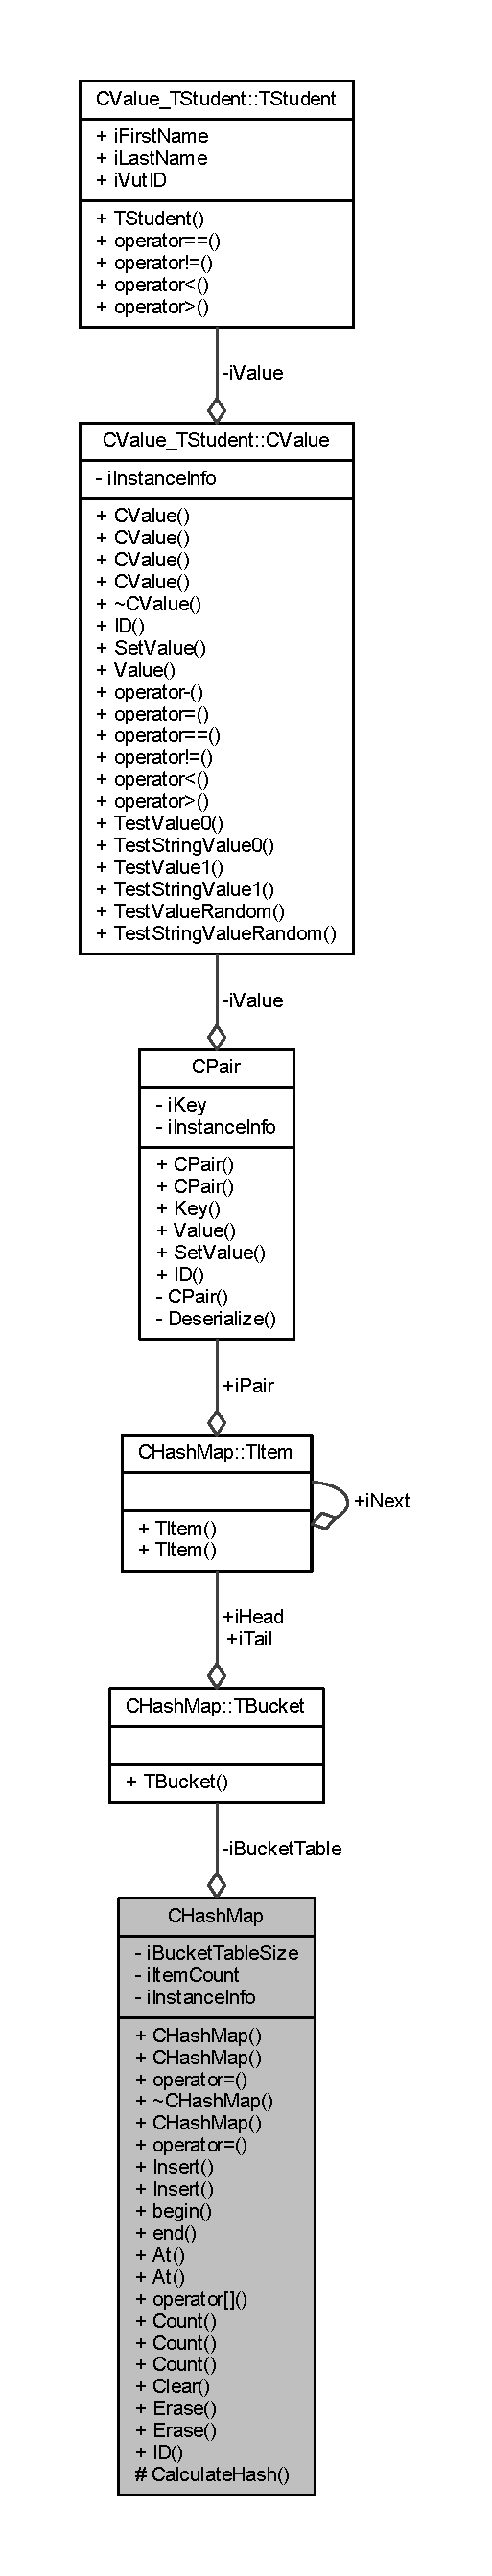
\includegraphics[height=550pt]{class_c_hash_map__coll__graph}
\end{center}
\end{figure}
\subsection*{Classes}
\begin{DoxyCompactItemize}
\item 
class \hyperlink{class_c_hash_map_1_1_c_forward_iterator}{C\+Forward\+Iterator}
\begin{DoxyCompactList}\small\item\em \hyperlink{class_c_hash_map_1_1_c_forward_iterator}{C\+Forward\+Iterator} class definition. \end{DoxyCompactList}\item 
struct \hyperlink{struct_c_hash_map_1_1_t_bucket}{T\+Bucket}
\begin{DoxyCompactList}\small\item\em \hyperlink{struct_c_hash_map_1_1_t_bucket}{T\+Bucket} structure definition. \end{DoxyCompactList}\item 
struct \hyperlink{struct_c_hash_map_1_1_t_item}{T\+Item}
\begin{DoxyCompactList}\small\item\em \hyperlink{struct_c_hash_map_1_1_t_item}{T\+Item} structure definiton. \end{DoxyCompactList}\end{DoxyCompactItemize}
\subsection*{Public Types}
\begin{DoxyCompactItemize}
\item 
enum \hyperlink{class_c_hash_map_ad4dd353df970a4464c449ef9f3b6a172}{T\+Insert} \{ \hyperlink{class_c_hash_map_ad4dd353df970a4464c449ef9f3b6a172a9823330641aba5e354b5ec054e03925d}{T\+Insert\+::\+E\+Unique\+Key} = 0, 
\hyperlink{class_c_hash_map_ad4dd353df970a4464c449ef9f3b6a172a21b083d0808068743c810401f5f3e416}{T\+Insert\+::\+E\+Before\+First\+Key\+Duplicity}, 
\hyperlink{class_c_hash_map_ad4dd353df970a4464c449ef9f3b6a172aecabac8c52e76e397328666a244c8df6}{T\+Insert\+::\+E\+After\+Last\+Key\+Duplicity}, 
\hyperlink{class_c_hash_map_ad4dd353df970a4464c449ef9f3b6a172a225fd4cd1da54b8b25b38434c9ef7078}{T\+Insert\+::\+E\+By\+Pair}
 \}\begin{DoxyCompactList}\small\item\em T\+Insert enumerator definition. \end{DoxyCompactList}
\item 
enum \hyperlink{class_c_hash_map_a9c8b9ae56d510ae0ff5e9ba74ee9930d}{T\+At} \{ \hyperlink{class_c_hash_map_a9c8b9ae56d510ae0ff5e9ba74ee9930da583fa6e6852d051c6e7f4b63cad9991f}{T\+At\+::\+E\+First\+Duplicity} = 0, 
\hyperlink{class_c_hash_map_a9c8b9ae56d510ae0ff5e9ba74ee9930da25f8a9e347bc7a066cf16ab19d17d12b}{T\+At\+::\+E\+Last\+Duplicity}
 \}\begin{DoxyCompactList}\small\item\em T\+At enumerator definition. \end{DoxyCompactList}
\end{DoxyCompactItemize}
\subsection*{Public Member Functions}
\begin{DoxyCompactItemize}
\item 
\hyperlink{class_c_hash_map_a40555c434d29ed0942ad03d41df3596d}{C\+Hash\+Map} (size\+\_\+t a\+Bucket\+Table\+Size=256)
\begin{DoxyCompactList}\small\item\em Implicit (and conversion) c\textquotesingle{}tor. \end{DoxyCompactList}\item 
\hyperlink{class_c_hash_map_afe589de62e80dde1ecf3fb606ce1a71f}{C\+Hash\+Map} (const \hyperlink{class_c_hash_map}{C\+Hash\+Map} \&a\+Hash\+Map)
\begin{DoxyCompactList}\small\item\em Copy c\textquotesingle{}tor. \end{DoxyCompactList}\item 
\hyperlink{class_c_hash_map}{C\+Hash\+Map} \& \hyperlink{class_c_hash_map_ac7b55d10283947ce6c4f0a7e73a0f80f}{operator=} (const \hyperlink{class_c_hash_map}{C\+Hash\+Map} \&a\+Hash\+Map)
\begin{DoxyCompactList}\small\item\em Assigment operator for maps. \end{DoxyCompactList}\item 
\hyperlink{class_c_hash_map_a74397f8f7751a170e3712d680a86de75}{$\sim$\+C\+Hash\+Map} ()
\begin{DoxyCompactList}\small\item\em d\textquotesingle{}tor \end{DoxyCompactList}\item 
\hyperlink{class_c_hash_map_a6640595075ccee64690e0ecaf9b4d4be}{C\+Hash\+Map} (\hyperlink{class_c_hash_map}{C\+Hash\+Map} \&\&)=default
\begin{DoxyCompactList}\small\item\em Default move c\textquotesingle{}tor. \end{DoxyCompactList}\item 
\hyperlink{class_c_hash_map}{C\+Hash\+Map} \& \hyperlink{class_c_hash_map_a3b494fb820ecd54937c05023fc67c564}{operator=} (\hyperlink{class_c_hash_map}{C\+Hash\+Map} \&\&)=default
\begin{DoxyCompactList}\small\item\em Default move assignment operator. \end{DoxyCompactList}\item 
\hyperlink{class_c_hash_map_1_1_c_forward_iterator}{C\+Forward\+Iterator} \hyperlink{class_c_hash_map_a443526f71277f329e9e77522c31f1350}{Insert} (const \hyperlink{class_c_pair}{C\+Pair} \&a\+Pair, \hyperlink{class_c_hash_map_ad4dd353df970a4464c449ef9f3b6a172}{T\+Insert} a\+Insert\+Mode=\hyperlink{class_c_hash_map_ad4dd353df970a4464c449ef9f3b6a172a9823330641aba5e354b5ec054e03925d}{T\+Insert\+::\+E\+Unique\+Key})
\begin{DoxyCompactList}\small\item\em Insert new pair to the map. \end{DoxyCompactList}\item 
\hyperlink{class_c_hash_map_1_1_c_forward_iterator}{C\+Forward\+Iterator} \hyperlink{class_c_hash_map_a0b9e79b3655b63c1f9a6d40715ad29fb}{Insert} (\hyperlink{class_c_pair}{C\+Pair} \&\&a\+Pair, \hyperlink{class_c_hash_map_ad4dd353df970a4464c449ef9f3b6a172}{T\+Insert} a\+Insert\+Mode=\hyperlink{class_c_hash_map_ad4dd353df970a4464c449ef9f3b6a172a9823330641aba5e354b5ec054e03925d}{T\+Insert\+::\+E\+Unique\+Key})
\begin{DoxyCompactList}\small\item\em Method Insert overload for move semantics. \end{DoxyCompactList}\item 
\hyperlink{class_c_hash_map_1_1_c_forward_iterator}{C\+Forward\+Iterator} \hyperlink{class_c_hash_map_ab7d482a398a96039875771b26624afdf}{begin} () const
\begin{DoxyCompactList}\small\item\em Create and return iterator pointing at first pair in the map. \end{DoxyCompactList}\item 
\hyperlink{class_c_hash_map_1_1_c_forward_iterator}{C\+Forward\+Iterator} \hyperlink{class_c_hash_map_a3129d3b5595237ab172fe060c072c376}{end} () const
\begin{DoxyCompactList}\small\item\em Create and return iterator pointing after last pair in the map. \end{DoxyCompactList}\item 
\hyperlink{class_c_hash_map_1_1_c_forward_iterator}{C\+Forward\+Iterator} \hyperlink{class_c_hash_map_a0819ba29ac861e3d948d94b12e315127}{At} (const \hyperlink{class_c_pair_a9030f3ef2a07301c105bdf17620ae66a}{C\+Pair\+::\+T\+Key} \&a\+Key, \hyperlink{class_c_hash_map_a9c8b9ae56d510ae0ff5e9ba74ee9930d}{T\+At} a\+At\+Mode=\hyperlink{class_c_hash_map_a9c8b9ae56d510ae0ff5e9ba74ee9930da583fa6e6852d051c6e7f4b63cad9991f}{T\+At\+::\+E\+First\+Duplicity}) const
\begin{DoxyCompactList}\small\item\em Create and return iterator pointing to pair with required key. \end{DoxyCompactList}\item 
\hyperlink{class_c_hash_map_1_1_c_forward_iterator}{C\+Forward\+Iterator} \hyperlink{class_c_hash_map_aed835e5c9cd93feab471205195fa749c}{At} (const \hyperlink{class_c_pair}{C\+Pair} \&a\+Pair, \hyperlink{class_c_hash_map_a9c8b9ae56d510ae0ff5e9ba74ee9930d}{T\+At} a\+At\+Mode=\hyperlink{class_c_hash_map_a9c8b9ae56d510ae0ff5e9ba74ee9930da583fa6e6852d051c6e7f4b63cad9991f}{T\+At\+::\+E\+First\+Duplicity}) const
\begin{DoxyCompactList}\small\item\em Create and return iterator pointing to the required pair. \end{DoxyCompactList}\item 
\hyperlink{class_c_pair}{C\+Pair} \& \hyperlink{class_c_hash_map_a4e61bb9cef654ff2377598e8d737a732}{operator\mbox{[}$\,$\mbox{]}} (const \hyperlink{class_c_pair_a9030f3ef2a07301c105bdf17620ae66a}{C\+Pair\+::\+T\+Key} \&a\+Key) const
\begin{DoxyCompactList}\small\item\em Indexing map by key (subscript operator) \end{DoxyCompactList}\item 
size\+\_\+t \hyperlink{class_c_hash_map_a331800dc9d92d201377132fe62c9c9cf}{Count} () const
\begin{DoxyCompactList}\small\item\em Pairs count getter. \end{DoxyCompactList}\item 
size\+\_\+t \hyperlink{class_c_hash_map_a00fac949f93212d8aef15740308b59e1}{Count} (const \hyperlink{class_c_pair_a9030f3ef2a07301c105bdf17620ae66a}{C\+Pair\+::\+T\+Key} \&a\+Key) const
\begin{DoxyCompactList}\small\item\em Pair with specific key count getter. \end{DoxyCompactList}\item 
size\+\_\+t \hyperlink{class_c_hash_map_a4fd67146fd24f86bbb686561a6326ce7}{Count} (const \hyperlink{class_c_pair}{C\+Pair} \&a\+Pair) const
\begin{DoxyCompactList}\small\item\em Pair with specific pair count getter. \end{DoxyCompactList}\item 
void \hyperlink{class_c_hash_map_a5fa63d790d41e91a0c61d63e813356af}{Clear} ()
\begin{DoxyCompactList}\small\item\em Clear content of the map. \end{DoxyCompactList}\item 
\hyperlink{class_c_hash_map_1_1_c_forward_iterator}{C\+Forward\+Iterator} \& \hyperlink{class_c_hash_map_a644b7450021eb6f1a7d2b03f7dbe1832}{Erase} (\hyperlink{class_c_hash_map_1_1_c_forward_iterator}{C\+Forward\+Iterator} \&a\+Iter)
\begin{DoxyCompactList}\small\item\em Erase pair pointed by \hyperlink{class_c_hash_map_1_1_c_forward_iterator}{C\+Forward\+Iterator}. \end{DoxyCompactList}\item 
\hyperlink{class_c_hash_map_1_1_c_forward_iterator}{C\+Forward\+Iterator} \&\& \hyperlink{class_c_hash_map_a82b22ccd322c826a368101e6451c5153}{Erase} (\hyperlink{class_c_hash_map_1_1_c_forward_iterator}{C\+Forward\+Iterator} \&\&a\+Iter)
\begin{DoxyCompactList}\small\item\em Method Erase overload for move semantics. \end{DoxyCompactList}\item 
size\+\_\+t \hyperlink{class_c_hash_map_a9db788f13512583b22ed7b75fd76a9de}{ID} () const
\begin{DoxyCompactList}\small\item\em Instance\+Info ID getter. \end{DoxyCompactList}\end{DoxyCompactItemize}
\subsection*{Protected Member Functions}
\begin{DoxyCompactItemize}
\item 
size\+\_\+t \hyperlink{class_c_hash_map_ad7230ba064063608b7e49495d3660426}{Calculate\+Hash} (const \hyperlink{class_c_pair_a9030f3ef2a07301c105bdf17620ae66a}{C\+Pair\+::\+T\+Key} \&a\+Key) const
\begin{DoxyCompactList}\small\item\em Hash value calculator. \end{DoxyCompactList}\end{DoxyCompactItemize}
\subsection*{Private Attributes}
\begin{DoxyCompactItemize}
\item 
\hyperlink{struct_c_hash_map_1_1_t_bucket}{T\+Bucket} $\ast$ \hyperlink{class_c_hash_map_a1018fdaad71e8207e747db26e88025d6}{i\+Bucket\+Table}
\begin{DoxyCompactList}\small\item\em Array of buckets (main datastructure of Hash\+Map) \end{DoxyCompactList}\item 
size\+\_\+t \hyperlink{class_c_hash_map_a8745c6aa08e235500828dea0ad30b548}{i\+Bucket\+Table\+Size}
\begin{DoxyCompactList}\small\item\em Number of the elements (buckets) in the {\ttfamily i\+Bucket\+Table}. \end{DoxyCompactList}\item 
size\+\_\+t \hyperlink{class_c_hash_map_aa1740c90e185ad56bf80632fc769c024}{i\+Item\+Count}
\begin{DoxyCompactList}\small\item\em Number of the pairs / items stored in the map. \end{DoxyCompactList}\item 
Class\+Info$<$ \hyperlink{class_c_hash_map}{C\+Hash\+Map} $>$ \hyperlink{class_c_hash_map_ae2e5e0311dc9a20f5a93c53a2fbfe9a2}{i\+Instance\+Info}
\begin{DoxyCompactList}\small\item\em Instance of the class info for usage statistics. \end{DoxyCompactList}\end{DoxyCompactItemize}


\subsection{Detailed Description}
\hyperlink{class_c_hash_map}{C\+Hash\+Map} class definition. 

Definition of \hyperlink{class_c_hash_map}{C\+Hash\+Map} class. There is defined all common methods and member variables. 

Definition at line 22 of file C\+Hash\+Map.\+h.



\subsection{Member Enumeration Documentation}
\mbox{\Hypertarget{class_c_hash_map_a9c8b9ae56d510ae0ff5e9ba74ee9930d}\label{class_c_hash_map_a9c8b9ae56d510ae0ff5e9ba74ee9930d}} 
\index{C\+Hash\+Map@{C\+Hash\+Map}!T\+At@{T\+At}}
\index{T\+At@{T\+At}!C\+Hash\+Map@{C\+Hash\+Map}}
\subsubsection{\texorpdfstring{T\+At}{TAt}}
{\footnotesize\ttfamily enum \hyperlink{class_c_hash_map_a9c8b9ae56d510ae0ff5e9ba74ee9930d}{C\+Hash\+Map\+::\+T\+At}\hspace{0.3cm}{\ttfamily [strong]}}



T\+At enumerator definition. 

Definition of T\+At enumerator used as parameter in the At methods. \begin{DoxyEnumFields}{Enumerator}
\raisebox{\heightof{T}}[0pt][0pt]{\index{E\+First\+Duplicity@{E\+First\+Duplicity}!C\+Hash\+Map@{C\+Hash\+Map}}\index{C\+Hash\+Map@{C\+Hash\+Map}!E\+First\+Duplicity@{E\+First\+Duplicity}}}\mbox{\Hypertarget{class_c_hash_map_a9c8b9ae56d510ae0ff5e9ba74ee9930da583fa6e6852d051c6e7f4b63cad9991f}\label{class_c_hash_map_a9c8b9ae56d510ae0ff5e9ba74ee9930da583fa6e6852d051c6e7f4b63cad9991f}} 
E\+First\+Duplicity&At returns iterator at first pair in the row of same keys. \\
\hline

\raisebox{\heightof{T}}[0pt][0pt]{\index{E\+Last\+Duplicity@{E\+Last\+Duplicity}!C\+Hash\+Map@{C\+Hash\+Map}}\index{C\+Hash\+Map@{C\+Hash\+Map}!E\+Last\+Duplicity@{E\+Last\+Duplicity}}}\mbox{\Hypertarget{class_c_hash_map_a9c8b9ae56d510ae0ff5e9ba74ee9930da25f8a9e347bc7a066cf16ab19d17d12b}\label{class_c_hash_map_a9c8b9ae56d510ae0ff5e9ba74ee9930da25f8a9e347bc7a066cf16ab19d17d12b}} 
E\+Last\+Duplicity&At returns iterator at lastt pair in the row of same keys. \\
\hline

\end{DoxyEnumFields}


Definition at line 39 of file C\+Hash\+Map.\+h.

\mbox{\Hypertarget{class_c_hash_map_ad4dd353df970a4464c449ef9f3b6a172}\label{class_c_hash_map_ad4dd353df970a4464c449ef9f3b6a172}} 
\index{C\+Hash\+Map@{C\+Hash\+Map}!T\+Insert@{T\+Insert}}
\index{T\+Insert@{T\+Insert}!C\+Hash\+Map@{C\+Hash\+Map}}
\subsubsection{\texorpdfstring{T\+Insert}{TInsert}}
{\footnotesize\ttfamily enum \hyperlink{class_c_hash_map_ad4dd353df970a4464c449ef9f3b6a172}{C\+Hash\+Map\+::\+T\+Insert}\hspace{0.3cm}{\ttfamily [strong]}}



T\+Insert enumerator definition. 

Definition of T\+Insert enumerator used as parameter in the Insert method. \begin{DoxyEnumFields}{Enumerator}
\raisebox{\heightof{T}}[0pt][0pt]{\index{E\+Unique\+Key@{E\+Unique\+Key}!C\+Hash\+Map@{C\+Hash\+Map}}\index{C\+Hash\+Map@{C\+Hash\+Map}!E\+Unique\+Key@{E\+Unique\+Key}}}\mbox{\Hypertarget{class_c_hash_map_ad4dd353df970a4464c449ef9f3b6a172a9823330641aba5e354b5ec054e03925d}\label{class_c_hash_map_ad4dd353df970a4464c449ef9f3b6a172a9823330641aba5e354b5ec054e03925d}} 
E\+Unique\+Key&Insert and check if key is Unique in the map. \\
\hline

\raisebox{\heightof{T}}[0pt][0pt]{\index{E\+Before\+First\+Key\+Duplicity@{E\+Before\+First\+Key\+Duplicity}!C\+Hash\+Map@{C\+Hash\+Map}}\index{C\+Hash\+Map@{C\+Hash\+Map}!E\+Before\+First\+Key\+Duplicity@{E\+Before\+First\+Key\+Duplicity}}}\mbox{\Hypertarget{class_c_hash_map_ad4dd353df970a4464c449ef9f3b6a172a21b083d0808068743c810401f5f3e416}\label{class_c_hash_map_ad4dd353df970a4464c449ef9f3b6a172a21b083d0808068743c810401f5f3e416}} 
E\+Before\+First\+Key\+Duplicity&Insert as first in the row of same keys. \\
\hline

\raisebox{\heightof{T}}[0pt][0pt]{\index{E\+After\+Last\+Key\+Duplicity@{E\+After\+Last\+Key\+Duplicity}!C\+Hash\+Map@{C\+Hash\+Map}}\index{C\+Hash\+Map@{C\+Hash\+Map}!E\+After\+Last\+Key\+Duplicity@{E\+After\+Last\+Key\+Duplicity}}}\mbox{\Hypertarget{class_c_hash_map_ad4dd353df970a4464c449ef9f3b6a172aecabac8c52e76e397328666a244c8df6}\label{class_c_hash_map_ad4dd353df970a4464c449ef9f3b6a172aecabac8c52e76e397328666a244c8df6}} 
E\+After\+Last\+Key\+Duplicity&Insert as last in the row of same keys. \\
\hline

\raisebox{\heightof{T}}[0pt][0pt]{\index{E\+By\+Pair@{E\+By\+Pair}!C\+Hash\+Map@{C\+Hash\+Map}}\index{C\+Hash\+Map@{C\+Hash\+Map}!E\+By\+Pair@{E\+By\+Pair}}}\mbox{\Hypertarget{class_c_hash_map_ad4dd353df970a4464c449ef9f3b6a172a225fd4cd1da54b8b25b38434c9ef7078}\label{class_c_hash_map_ad4dd353df970a4464c449ef9f3b6a172a225fd4cd1da54b8b25b38434c9ef7078}} 
E\+By\+Pair&Insert in the row of same keys after pair with less or same value. \\
\hline

\end{DoxyEnumFields}


Definition at line 28 of file C\+Hash\+Map.\+h.



\subsection{Constructor \& Destructor Documentation}
\mbox{\Hypertarget{class_c_hash_map_a40555c434d29ed0942ad03d41df3596d}\label{class_c_hash_map_a40555c434d29ed0942ad03d41df3596d}} 
\index{C\+Hash\+Map@{C\+Hash\+Map}!C\+Hash\+Map@{C\+Hash\+Map}}
\index{C\+Hash\+Map@{C\+Hash\+Map}!C\+Hash\+Map@{C\+Hash\+Map}}
\subsubsection{\texorpdfstring{C\+Hash\+Map()}{CHashMap()}\hspace{0.1cm}{\footnotesize\ttfamily [1/3]}}
{\footnotesize\ttfamily C\+Hash\+Map\+::\+C\+Hash\+Map (\begin{DoxyParamCaption}\item[{size\+\_\+t}]{a\+Bucket\+Table\+Size = {\ttfamily 256} }\end{DoxyParamCaption})\hspace{0.3cm}{\ttfamily [inline]}}



Implicit (and conversion) c\textquotesingle{}tor. 

Create empty map with defined number of buckets 
\begin{DoxyParams}[1]{Parameters}
\mbox{\tt in}  & {\em a\+Bucket\+Table\+Size} & Number of Bucket in the internal hash map structures (implicit value is 256) \\
\hline
\end{DoxyParams}
\begin{DoxyAttention}{Attention}
C\textquotesingle{}tor generate {\ttfamily std\+::length\+\_\+error} exception if {\itshape a\+Bucket\+Table\+Size} is less than 2 
\end{DoxyAttention}


Definition at line 202 of file C\+Hash\+Map.\+h.

\mbox{\Hypertarget{class_c_hash_map_afe589de62e80dde1ecf3fb606ce1a71f}\label{class_c_hash_map_afe589de62e80dde1ecf3fb606ce1a71f}} 
\index{C\+Hash\+Map@{C\+Hash\+Map}!C\+Hash\+Map@{C\+Hash\+Map}}
\index{C\+Hash\+Map@{C\+Hash\+Map}!C\+Hash\+Map@{C\+Hash\+Map}}
\subsubsection{\texorpdfstring{C\+Hash\+Map()}{CHashMap()}\hspace{0.1cm}{\footnotesize\ttfamily [2/3]}}
{\footnotesize\ttfamily C\+Hash\+Map\+::\+C\+Hash\+Map (\begin{DoxyParamCaption}\item[{const \hyperlink{class_c_hash_map}{C\+Hash\+Map} \&}]{a\+Hash\+Map }\end{DoxyParamCaption})}



Copy c\textquotesingle{}tor. 

Create deep copy of the {\itshape a\+Hash\+Map} the to new map instance 
\begin{DoxyParams}[1]{Parameters}
\mbox{\tt in}  & {\em a\+Hash\+Map} & Source map used for copying \\
\hline
\end{DoxyParams}


Definition at line 45 of file C\+Hash\+Map.\+cpp.

\mbox{\Hypertarget{class_c_hash_map_a74397f8f7751a170e3712d680a86de75}\label{class_c_hash_map_a74397f8f7751a170e3712d680a86de75}} 
\index{C\+Hash\+Map@{C\+Hash\+Map}!````~C\+Hash\+Map@{$\sim$\+C\+Hash\+Map}}
\index{````~C\+Hash\+Map@{$\sim$\+C\+Hash\+Map}!C\+Hash\+Map@{C\+Hash\+Map}}
\subsubsection{\texorpdfstring{$\sim$\+C\+Hash\+Map()}{~CHashMap()}}
{\footnotesize\ttfamily C\+Hash\+Map\+::$\sim$\+C\+Hash\+Map (\begin{DoxyParamCaption}{ }\end{DoxyParamCaption})\hspace{0.3cm}{\ttfamily [inline]}}



d\textquotesingle{}tor 

Clear and deallocate all items in the each bucket 

Definition at line 224 of file C\+Hash\+Map.\+h.

\mbox{\Hypertarget{class_c_hash_map_a6640595075ccee64690e0ecaf9b4d4be}\label{class_c_hash_map_a6640595075ccee64690e0ecaf9b4d4be}} 
\index{C\+Hash\+Map@{C\+Hash\+Map}!C\+Hash\+Map@{C\+Hash\+Map}}
\index{C\+Hash\+Map@{C\+Hash\+Map}!C\+Hash\+Map@{C\+Hash\+Map}}
\subsubsection{\texorpdfstring{C\+Hash\+Map()}{CHashMap()}\hspace{0.1cm}{\footnotesize\ttfamily [3/3]}}
{\footnotesize\ttfamily C\+Hash\+Map\+::\+C\+Hash\+Map (\begin{DoxyParamCaption}\item[{\hyperlink{class_c_hash_map}{C\+Hash\+Map} \&\&}]{ }\end{DoxyParamCaption})\hspace{0.3cm}{\ttfamily [default]}}



Default move c\textquotesingle{}tor. 

Move content of the one map to the new map instance 

\subsection{Member Function Documentation}
\mbox{\Hypertarget{class_c_hash_map_a0819ba29ac861e3d948d94b12e315127}\label{class_c_hash_map_a0819ba29ac861e3d948d94b12e315127}} 
\index{C\+Hash\+Map@{C\+Hash\+Map}!At@{At}}
\index{At@{At}!C\+Hash\+Map@{C\+Hash\+Map}}
\subsubsection{\texorpdfstring{At()}{At()}\hspace{0.1cm}{\footnotesize\ttfamily [1/2]}}
{\footnotesize\ttfamily \hyperlink{class_c_hash_map_1_1_c_forward_iterator}{C\+Hash\+Map\+::\+C\+Forward\+Iterator} C\+Hash\+Map\+::\+At (\begin{DoxyParamCaption}\item[{const \hyperlink{class_c_pair_a9030f3ef2a07301c105bdf17620ae66a}{C\+Pair\+::\+T\+Key} \&}]{a\+Key,  }\item[{\hyperlink{class_c_hash_map_a9c8b9ae56d510ae0ff5e9ba74ee9930d}{T\+At}}]{a\+At\+Mode = {\ttfamily \hyperlink{class_c_hash_map_a9c8b9ae56d510ae0ff5e9ba74ee9930da583fa6e6852d051c6e7f4b63cad9991f}{T\+At\+::\+E\+First\+Duplicity}} }\end{DoxyParamCaption}) const}



Create and return iterator pointing to pair with required key. 


\begin{DoxyParams}[1]{Parameters}
\mbox{\tt in}  & {\em a\+Key} & Required key \\
\hline
\mbox{\tt in}  & {\em a\+At\+Mode} & Mode of finding required pair (implicit mode is \hyperlink{class_c_hash_map_a9c8b9ae56d510ae0ff5e9ba74ee9930da583fa6e6852d051c6e7f4b63cad9991f}{T\+At\+::\+E\+First\+Duplicity}) \\
\hline
\end{DoxyParams}
\begin{DoxyReturn}{Returns}
Iterator pointing to the required pair 
\end{DoxyReturn}


Definition at line 145 of file C\+Hash\+Map.\+cpp.

\mbox{\Hypertarget{class_c_hash_map_aed835e5c9cd93feab471205195fa749c}\label{class_c_hash_map_aed835e5c9cd93feab471205195fa749c}} 
\index{C\+Hash\+Map@{C\+Hash\+Map}!At@{At}}
\index{At@{At}!C\+Hash\+Map@{C\+Hash\+Map}}
\subsubsection{\texorpdfstring{At()}{At()}\hspace{0.1cm}{\footnotesize\ttfamily [2/2]}}
{\footnotesize\ttfamily \hyperlink{class_c_hash_map_1_1_c_forward_iterator}{C\+Hash\+Map\+::\+C\+Forward\+Iterator} C\+Hash\+Map\+::\+At (\begin{DoxyParamCaption}\item[{const \hyperlink{class_c_pair}{C\+Pair} \&}]{a\+Pair,  }\item[{\hyperlink{class_c_hash_map_a9c8b9ae56d510ae0ff5e9ba74ee9930d}{T\+At}}]{a\+At\+Mode = {\ttfamily \hyperlink{class_c_hash_map_a9c8b9ae56d510ae0ff5e9ba74ee9930da583fa6e6852d051c6e7f4b63cad9991f}{T\+At\+::\+E\+First\+Duplicity}} }\end{DoxyParamCaption}) const}



Create and return iterator pointing to the required pair. 


\begin{DoxyParams}[1]{Parameters}
\mbox{\tt in}  & {\em a\+Pair} & Required pair (key and value) \\
\hline
\mbox{\tt in}  & {\em a\+At\+Mode} & Mode of finding required pair (implicit mode is \hyperlink{class_c_hash_map_a9c8b9ae56d510ae0ff5e9ba74ee9930da583fa6e6852d051c6e7f4b63cad9991f}{T\+At\+::\+E\+First\+Duplicity}) \\
\hline
\end{DoxyParams}
\begin{DoxyReturn}{Returns}
Iterator pointing to the required pair 
\end{DoxyReturn}


Definition at line 177 of file C\+Hash\+Map.\+cpp.

\mbox{\Hypertarget{class_c_hash_map_ab7d482a398a96039875771b26624afdf}\label{class_c_hash_map_ab7d482a398a96039875771b26624afdf}} 
\index{C\+Hash\+Map@{C\+Hash\+Map}!begin@{begin}}
\index{begin@{begin}!C\+Hash\+Map@{C\+Hash\+Map}}
\subsubsection{\texorpdfstring{begin()}{begin()}}
{\footnotesize\ttfamily \hyperlink{class_c_hash_map_1_1_c_forward_iterator}{C\+Hash\+Map\+::\+C\+Forward\+Iterator} C\+Hash\+Map\+::begin (\begin{DoxyParamCaption}{ }\end{DoxyParamCaption}) const}



Create and return iterator pointing at first pair in the map. 

\begin{DoxyReturn}{Returns}
Iterator pointing at first pair in the map 
\end{DoxyReturn}


Definition at line 130 of file C\+Hash\+Map.\+cpp.

\mbox{\Hypertarget{class_c_hash_map_ad7230ba064063608b7e49495d3660426}\label{class_c_hash_map_ad7230ba064063608b7e49495d3660426}} 
\index{C\+Hash\+Map@{C\+Hash\+Map}!Calculate\+Hash@{Calculate\+Hash}}
\index{Calculate\+Hash@{Calculate\+Hash}!C\+Hash\+Map@{C\+Hash\+Map}}
\subsubsection{\texorpdfstring{Calculate\+Hash()}{CalculateHash()}}
{\footnotesize\ttfamily size\+\_\+t C\+Hash\+Map\+::\+Calculate\+Hash (\begin{DoxyParamCaption}\item[{const \hyperlink{class_c_pair_a9030f3ef2a07301c105bdf17620ae66a}{C\+Pair\+::\+T\+Key} \&}]{a\+Key }\end{DoxyParamCaption}) const\hspace{0.3cm}{\ttfamily [inline]}, {\ttfamily [protected]}}



Hash value calculator. 


\begin{DoxyParams}[1]{Parameters}
\mbox{\tt in}  & {\em a\+Key} & Key value \\
\hline
\end{DoxyParams}
\begin{DoxyReturn}{Returns}
Hash value (bucket index) calculated from {\itshape a\+Key} and {\ttfamily i\+Bucket\+Table\+Size} 
\end{DoxyReturn}


Definition at line 112 of file C\+Hash\+Map.\+h.

\mbox{\Hypertarget{class_c_hash_map_a5fa63d790d41e91a0c61d63e813356af}\label{class_c_hash_map_a5fa63d790d41e91a0c61d63e813356af}} 
\index{C\+Hash\+Map@{C\+Hash\+Map}!Clear@{Clear}}
\index{Clear@{Clear}!C\+Hash\+Map@{C\+Hash\+Map}}
\subsubsection{\texorpdfstring{Clear()}{Clear()}}
{\footnotesize\ttfamily void C\+Hash\+Map\+::\+Clear (\begin{DoxyParamCaption}{ }\end{DoxyParamCaption})}



Clear content of the map. 

Deallocate all Item with Pairs, Bucket\+Table and initialize as empty whole Map 

Definition at line 234 of file C\+Hash\+Map.\+cpp.

\mbox{\Hypertarget{class_c_hash_map_a331800dc9d92d201377132fe62c9c9cf}\label{class_c_hash_map_a331800dc9d92d201377132fe62c9c9cf}} 
\index{C\+Hash\+Map@{C\+Hash\+Map}!Count@{Count}}
\index{Count@{Count}!C\+Hash\+Map@{C\+Hash\+Map}}
\subsubsection{\texorpdfstring{Count()}{Count()}\hspace{0.1cm}{\footnotesize\ttfamily [1/3]}}
{\footnotesize\ttfamily size\+\_\+t C\+Hash\+Map\+::\+Count (\begin{DoxyParamCaption}{ }\end{DoxyParamCaption}) const\hspace{0.3cm}{\ttfamily [inline]}}



Pairs count getter. 

\begin{DoxyReturn}{Returns}
Number of pairs stored in the \hyperlink{class_c_hash_map}{C\+Hash\+Map} 
\end{DoxyReturn}


Definition at line 290 of file C\+Hash\+Map.\+h.

\mbox{\Hypertarget{class_c_hash_map_a00fac949f93212d8aef15740308b59e1}\label{class_c_hash_map_a00fac949f93212d8aef15740308b59e1}} 
\index{C\+Hash\+Map@{C\+Hash\+Map}!Count@{Count}}
\index{Count@{Count}!C\+Hash\+Map@{C\+Hash\+Map}}
\subsubsection{\texorpdfstring{Count()}{Count()}\hspace{0.1cm}{\footnotesize\ttfamily [2/3]}}
{\footnotesize\ttfamily size\+\_\+t C\+Hash\+Map\+::\+Count (\begin{DoxyParamCaption}\item[{const \hyperlink{class_c_pair_a9030f3ef2a07301c105bdf17620ae66a}{C\+Pair\+::\+T\+Key} \&}]{a\+Key }\end{DoxyParamCaption}) const}



Pair with specific key count getter. 


\begin{DoxyParams}[1]{Parameters}
\mbox{\tt in}  & {\em a\+Key} & Key value \\
\hline
\end{DoxyParams}
\begin{DoxyReturn}{Returns}
Number of pairs stored in the \hyperlink{class_c_hash_map}{C\+Hash\+Map} with key equals to {\itshape a\+Key} 
\end{DoxyReturn}


Definition at line 216 of file C\+Hash\+Map.\+cpp.

\mbox{\Hypertarget{class_c_hash_map_a4fd67146fd24f86bbb686561a6326ce7}\label{class_c_hash_map_a4fd67146fd24f86bbb686561a6326ce7}} 
\index{C\+Hash\+Map@{C\+Hash\+Map}!Count@{Count}}
\index{Count@{Count}!C\+Hash\+Map@{C\+Hash\+Map}}
\subsubsection{\texorpdfstring{Count()}{Count()}\hspace{0.1cm}{\footnotesize\ttfamily [3/3]}}
{\footnotesize\ttfamily size\+\_\+t C\+Hash\+Map\+::\+Count (\begin{DoxyParamCaption}\item[{const \hyperlink{class_c_pair}{C\+Pair} \&}]{a\+Pair }\end{DoxyParamCaption}) const}



Pair with specific pair count getter. 


\begin{DoxyParams}[1]{Parameters}
\mbox{\tt in}  & {\em a\+Pair} & Pair value \\
\hline
\end{DoxyParams}
\begin{DoxyReturn}{Returns}
Number of pairs stored in the \hyperlink{class_c_hash_map}{C\+Hash\+Map} with key and Value equals to {\itshape a\+Pair} 
\end{DoxyReturn}


Definition at line 224 of file C\+Hash\+Map.\+cpp.

\mbox{\Hypertarget{class_c_hash_map_a3129d3b5595237ab172fe060c072c376}\label{class_c_hash_map_a3129d3b5595237ab172fe060c072c376}} 
\index{C\+Hash\+Map@{C\+Hash\+Map}!end@{end}}
\index{end@{end}!C\+Hash\+Map@{C\+Hash\+Map}}
\subsubsection{\texorpdfstring{end()}{end()}}
{\footnotesize\ttfamily \hyperlink{class_c_hash_map_1_1_c_forward_iterator}{C\+Forward\+Iterator} C\+Hash\+Map\+::end (\begin{DoxyParamCaption}{ }\end{DoxyParamCaption}) const\hspace{0.3cm}{\ttfamily [inline]}}



Create and return iterator pointing after last pair in the map. 

\begin{DoxyReturn}{Returns}
Iterator pointing after last pair in the map 
\end{DoxyReturn}


Definition at line 263 of file C\+Hash\+Map.\+h.

\mbox{\Hypertarget{class_c_hash_map_a644b7450021eb6f1a7d2b03f7dbe1832}\label{class_c_hash_map_a644b7450021eb6f1a7d2b03f7dbe1832}} 
\index{C\+Hash\+Map@{C\+Hash\+Map}!Erase@{Erase}}
\index{Erase@{Erase}!C\+Hash\+Map@{C\+Hash\+Map}}
\subsubsection{\texorpdfstring{Erase()}{Erase()}\hspace{0.1cm}{\footnotesize\ttfamily [1/2]}}
{\footnotesize\ttfamily \hyperlink{class_c_hash_map_1_1_c_forward_iterator}{C\+Hash\+Map\+::\+C\+Forward\+Iterator} \& C\+Hash\+Map\+::\+Erase (\begin{DoxyParamCaption}\item[{\hyperlink{class_c_hash_map_1_1_c_forward_iterator}{C\+Hash\+Map\+::\+C\+Forward\+Iterator} \&}]{a\+Iter }\end{DoxyParamCaption})}



Erase pair pointed by \hyperlink{class_c_hash_map_1_1_c_forward_iterator}{C\+Forward\+Iterator}. 

Erase pair of the \hyperlink{class_c_hash_map}{C\+Hash\+Map} which is pointing by \hyperlink{class_c_hash_map_1_1_c_forward_iterator}{C\+Forward\+Iterator}. {\itshape a\+Iter} must point to the pairs in the same map. 
\begin{DoxyParams}[1]{Parameters}
\mbox{\tt in,out}  & {\em a\+Iter} & Iterator pointing to the pair value in the \hyperlink{class_c_hash_map}{C\+Hash\+Map}. Method update {\itshape a\+Iter} after removing Pair to the new valid value. \\
\hline
\end{DoxyParams}
\begin{DoxyReturn}{Returns}
New valid value of iterator. Iterator now pointing to the pair after removed pair if there exist. 
\end{DoxyReturn}
\begin{DoxyAttention}{Attention}
Method generate {\ttfamily std\+::runtime\+\_\+error} exception if {\itshape a\+Iter} is invalid iterator (nullptr) 

Method generate {\ttfamily std\+::logic\+\_\+error} exception if {\itshape a\+Iter} pointing to the different Hash\+Map than is associated with {\ttfamily this} 
\end{DoxyAttention}


Definition at line 254 of file C\+Hash\+Map.\+cpp.

\mbox{\Hypertarget{class_c_hash_map_a82b22ccd322c826a368101e6451c5153}\label{class_c_hash_map_a82b22ccd322c826a368101e6451c5153}} 
\index{C\+Hash\+Map@{C\+Hash\+Map}!Erase@{Erase}}
\index{Erase@{Erase}!C\+Hash\+Map@{C\+Hash\+Map}}
\subsubsection{\texorpdfstring{Erase()}{Erase()}\hspace{0.1cm}{\footnotesize\ttfamily [2/2]}}
{\footnotesize\ttfamily \hyperlink{class_c_hash_map_1_1_c_forward_iterator}{C\+Forward\+Iterator}\&\& C\+Hash\+Map\+::\+Erase (\begin{DoxyParamCaption}\item[{\hyperlink{class_c_hash_map_1_1_c_forward_iterator}{C\+Forward\+Iterator} \&\&}]{a\+Iter }\end{DoxyParamCaption})\hspace{0.3cm}{\ttfamily [inline]}}



Method Erase overload for move semantics. 



Definition at line 321 of file C\+Hash\+Map.\+h.

\mbox{\Hypertarget{class_c_hash_map_a9db788f13512583b22ed7b75fd76a9de}\label{class_c_hash_map_a9db788f13512583b22ed7b75fd76a9de}} 
\index{C\+Hash\+Map@{C\+Hash\+Map}!ID@{ID}}
\index{ID@{ID}!C\+Hash\+Map@{C\+Hash\+Map}}
\subsubsection{\texorpdfstring{I\+D()}{ID()}}
{\footnotesize\ttfamily size\+\_\+t C\+Hash\+Map\+::\+ID (\begin{DoxyParamCaption}{ }\end{DoxyParamCaption}) const\hspace{0.3cm}{\ttfamily [inline]}}



Instance\+Info ID getter. 

\begin{DoxyReturn}{Returns}
Unique instance ID 
\end{DoxyReturn}


Definition at line 327 of file C\+Hash\+Map.\+h.

\mbox{\Hypertarget{class_c_hash_map_a443526f71277f329e9e77522c31f1350}\label{class_c_hash_map_a443526f71277f329e9e77522c31f1350}} 
\index{C\+Hash\+Map@{C\+Hash\+Map}!Insert@{Insert}}
\index{Insert@{Insert}!C\+Hash\+Map@{C\+Hash\+Map}}
\subsubsection{\texorpdfstring{Insert()}{Insert()}\hspace{0.1cm}{\footnotesize\ttfamily [1/2]}}
{\footnotesize\ttfamily \hyperlink{class_c_hash_map_1_1_c_forward_iterator}{C\+Forward\+Iterator} C\+Hash\+Map\+::\+Insert (\begin{DoxyParamCaption}\item[{const \hyperlink{class_c_pair}{C\+Pair} \&}]{a\+Pair,  }\item[{\hyperlink{class_c_hash_map_ad4dd353df970a4464c449ef9f3b6a172}{T\+Insert}}]{a\+Insert\+Mode = {\ttfamily \hyperlink{class_c_hash_map_ad4dd353df970a4464c449ef9f3b6a172a9823330641aba5e354b5ec054e03925d}{T\+Insert\+::\+E\+Unique\+Key}} }\end{DoxyParamCaption})\hspace{0.3cm}{\ttfamily [inline]}}



Insert new pair to the map. 

Use key and value to create new (copying) pair and insert it into the map 
\begin{DoxyParams}[1]{Parameters}
\mbox{\tt in}  & {\em a\+Pair} & Pair for inserting \\
\hline
\mbox{\tt in}  & {\em a\+Insert\+Mode} & Mode of insertion new pair (implicit mode is \hyperlink{class_c_hash_map_ad4dd353df970a4464c449ef9f3b6a172a9823330641aba5e354b5ec054e03925d}{T\+Insert\+::\+E\+Unique\+Key}) \\
\hline
\end{DoxyParams}
\begin{DoxyReturn}{Returns}
Iterator pointing to the inserted pair 
\end{DoxyReturn}
\begin{DoxyAttention}{Attention}
Method generate {\ttfamily std\+::runtime\+\_\+error} exception if insertion mode is {\ttfamily E\+Unique\+Key} and {\itshape a\+Key} in the map already exist 
\end{DoxyAttention}


Definition at line 247 of file C\+Hash\+Map.\+h.

\mbox{\Hypertarget{class_c_hash_map_a0b9e79b3655b63c1f9a6d40715ad29fb}\label{class_c_hash_map_a0b9e79b3655b63c1f9a6d40715ad29fb}} 
\index{C\+Hash\+Map@{C\+Hash\+Map}!Insert@{Insert}}
\index{Insert@{Insert}!C\+Hash\+Map@{C\+Hash\+Map}}
\subsubsection{\texorpdfstring{Insert()}{Insert()}\hspace{0.1cm}{\footnotesize\ttfamily [2/2]}}
{\footnotesize\ttfamily \hyperlink{class_c_hash_map_1_1_c_forward_iterator}{C\+Hash\+Map\+::\+C\+Forward\+Iterator} C\+Hash\+Map\+::\+Insert (\begin{DoxyParamCaption}\item[{\hyperlink{class_c_pair}{C\+Pair} \&\&}]{a\+Pair,  }\item[{\hyperlink{class_c_hash_map_ad4dd353df970a4464c449ef9f3b6a172}{T\+Insert}}]{a\+Insert\+Mode = {\ttfamily \hyperlink{class_c_hash_map_ad4dd353df970a4464c449ef9f3b6a172a9823330641aba5e354b5ec054e03925d}{T\+Insert\+::\+E\+Unique\+Key}} }\end{DoxyParamCaption})}



Method Insert overload for move semantics. 

Use key and value to create new (moving) pair and insert it into the map 

Definition at line 75 of file C\+Hash\+Map.\+cpp.

\mbox{\Hypertarget{class_c_hash_map_ac7b55d10283947ce6c4f0a7e73a0f80f}\label{class_c_hash_map_ac7b55d10283947ce6c4f0a7e73a0f80f}} 
\index{C\+Hash\+Map@{C\+Hash\+Map}!operator=@{operator=}}
\index{operator=@{operator=}!C\+Hash\+Map@{C\+Hash\+Map}}
\subsubsection{\texorpdfstring{operator=()}{operator=()}\hspace{0.1cm}{\footnotesize\ttfamily [1/2]}}
{\footnotesize\ttfamily \hyperlink{class_c_hash_map}{C\+Hash\+Map} \& C\+Hash\+Map\+::operator= (\begin{DoxyParamCaption}\item[{const \hyperlink{class_c_hash_map}{C\+Hash\+Map} \&}]{a\+Hash\+Map }\end{DoxyParamCaption})}



Assigment operator for maps. 

Remove previous content of the map ane made deep copy of {\itshape a\+Hash\+Map} 
\begin{DoxyParams}[1]{Parameters}
\mbox{\tt in}  & {\em a\+Hash\+Map} & Source map used for copying \\
\hline
\end{DoxyParams}
\begin{DoxyReturn}{Returns}
Reference to self 
\end{DoxyReturn}


Definition at line 56 of file C\+Hash\+Map.\+cpp.

\mbox{\Hypertarget{class_c_hash_map_a3b494fb820ecd54937c05023fc67c564}\label{class_c_hash_map_a3b494fb820ecd54937c05023fc67c564}} 
\index{C\+Hash\+Map@{C\+Hash\+Map}!operator=@{operator=}}
\index{operator=@{operator=}!C\+Hash\+Map@{C\+Hash\+Map}}
\subsubsection{\texorpdfstring{operator=()}{operator=()}\hspace{0.1cm}{\footnotesize\ttfamily [2/2]}}
{\footnotesize\ttfamily \hyperlink{class_c_hash_map}{C\+Hash\+Map}\& C\+Hash\+Map\+::operator= (\begin{DoxyParamCaption}\item[{\hyperlink{class_c_hash_map}{C\+Hash\+Map} \&\&}]{ }\end{DoxyParamCaption})\hspace{0.3cm}{\ttfamily [default]}}



Default move assignment operator. 

Move content of the one map to the other map instance \mbox{\Hypertarget{class_c_hash_map_a4e61bb9cef654ff2377598e8d737a732}\label{class_c_hash_map_a4e61bb9cef654ff2377598e8d737a732}} 
\index{C\+Hash\+Map@{C\+Hash\+Map}!operator\mbox{[}\mbox{]}@{operator[]}}
\index{operator\mbox{[}\mbox{]}@{operator[]}!C\+Hash\+Map@{C\+Hash\+Map}}
\subsubsection{\texorpdfstring{operator[]()}{operator[]()}}
{\footnotesize\ttfamily \hyperlink{class_c_pair}{C\+Pair} \& C\+Hash\+Map\+::operator\mbox{[}$\,$\mbox{]} (\begin{DoxyParamCaption}\item[{const \hyperlink{class_c_pair_a9030f3ef2a07301c105bdf17620ae66a}{C\+Pair\+::\+T\+Key} \&}]{a\+Key }\end{DoxyParamCaption}) const}



Indexing map by key (subscript operator) 


\begin{DoxyParams}[1]{Parameters}
\mbox{\tt in}  & {\em a\+Key} & Key value \\
\hline
\end{DoxyParams}
\begin{DoxyReturn}{Returns}
reference to first pair with required {\itshape a\+Key} 
\end{DoxyReturn}
\begin{DoxyAttention}{Attention}
Method generate {\ttfamily std\+::runtime\+\_\+error} exception if {\itshape a\+Key} in the map does not exist 
\end{DoxyAttention}


Definition at line 207 of file C\+Hash\+Map.\+cpp.



\subsection{Member Data Documentation}
\mbox{\Hypertarget{class_c_hash_map_a1018fdaad71e8207e747db26e88025d6}\label{class_c_hash_map_a1018fdaad71e8207e747db26e88025d6}} 
\index{C\+Hash\+Map@{C\+Hash\+Map}!i\+Bucket\+Table@{i\+Bucket\+Table}}
\index{i\+Bucket\+Table@{i\+Bucket\+Table}!C\+Hash\+Map@{C\+Hash\+Map}}
\subsubsection{\texorpdfstring{i\+Bucket\+Table}{iBucketTable}}
{\footnotesize\ttfamily \hyperlink{struct_c_hash_map_1_1_t_bucket}{T\+Bucket}$\ast$ C\+Hash\+Map\+::i\+Bucket\+Table\hspace{0.3cm}{\ttfamily [private]}}



Array of buckets (main datastructure of Hash\+Map) 



Definition at line 102 of file C\+Hash\+Map.\+h.

\mbox{\Hypertarget{class_c_hash_map_a8745c6aa08e235500828dea0ad30b548}\label{class_c_hash_map_a8745c6aa08e235500828dea0ad30b548}} 
\index{C\+Hash\+Map@{C\+Hash\+Map}!i\+Bucket\+Table\+Size@{i\+Bucket\+Table\+Size}}
\index{i\+Bucket\+Table\+Size@{i\+Bucket\+Table\+Size}!C\+Hash\+Map@{C\+Hash\+Map}}
\subsubsection{\texorpdfstring{i\+Bucket\+Table\+Size}{iBucketTableSize}}
{\footnotesize\ttfamily size\+\_\+t C\+Hash\+Map\+::i\+Bucket\+Table\+Size\hspace{0.3cm}{\ttfamily [private]}}



Number of the elements (buckets) in the {\ttfamily i\+Bucket\+Table}. 



Definition at line 103 of file C\+Hash\+Map.\+h.

\mbox{\Hypertarget{class_c_hash_map_ae2e5e0311dc9a20f5a93c53a2fbfe9a2}\label{class_c_hash_map_ae2e5e0311dc9a20f5a93c53a2fbfe9a2}} 
\index{C\+Hash\+Map@{C\+Hash\+Map}!i\+Instance\+Info@{i\+Instance\+Info}}
\index{i\+Instance\+Info@{i\+Instance\+Info}!C\+Hash\+Map@{C\+Hash\+Map}}
\subsubsection{\texorpdfstring{i\+Instance\+Info}{iInstanceInfo}}
{\footnotesize\ttfamily Class\+Info$<$\hyperlink{class_c_hash_map}{C\+Hash\+Map}$>$ C\+Hash\+Map\+::i\+Instance\+Info\hspace{0.3cm}{\ttfamily [private]}}



Instance of the class info for usage statistics. 



Definition at line 105 of file C\+Hash\+Map.\+h.

\mbox{\Hypertarget{class_c_hash_map_aa1740c90e185ad56bf80632fc769c024}\label{class_c_hash_map_aa1740c90e185ad56bf80632fc769c024}} 
\index{C\+Hash\+Map@{C\+Hash\+Map}!i\+Item\+Count@{i\+Item\+Count}}
\index{i\+Item\+Count@{i\+Item\+Count}!C\+Hash\+Map@{C\+Hash\+Map}}
\subsubsection{\texorpdfstring{i\+Item\+Count}{iItemCount}}
{\footnotesize\ttfamily size\+\_\+t C\+Hash\+Map\+::i\+Item\+Count\hspace{0.3cm}{\ttfamily [private]}}



Number of the pairs / items stored in the map. 



Definition at line 104 of file C\+Hash\+Map.\+h.



The documentation for this class was generated from the following files\+:\begin{DoxyCompactItemize}
\item 
\hyperlink{_c_hash_map_8h}{C\+Hash\+Map.\+h}\item 
\hyperlink{_c_hash_map_8cpp}{C\+Hash\+Map.\+cpp}\end{DoxyCompactItemize}

\hypertarget{class_c_pair}{}\section{C\+Pair Class Reference}
\label{class_c_pair}\index{C\+Pair@{C\+Pair}}


\hyperlink{class_c_pair}{C\+Pair} class (key and value)  




{\ttfamily \#include $<$C\+Pair.\+h$>$}



Collaboration diagram for C\+Pair\+:
\nopagebreak
\begin{figure}[H]
\begin{center}
\leavevmode
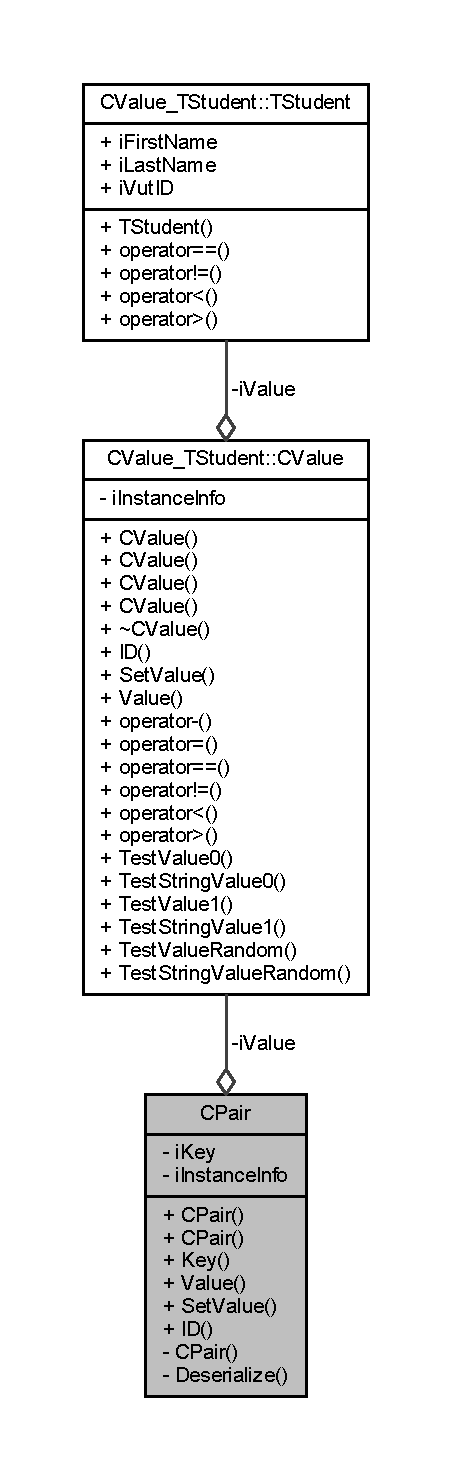
\includegraphics[height=550pt]{class_c_pair__coll__graph}
\end{center}
\end{figure}
\subsection*{Public Types}
\begin{DoxyCompactItemize}
\item 
using \hyperlink{class_c_pair_a9030f3ef2a07301c105bdf17620ae66a}{T\+Key} = int
\end{DoxyCompactItemize}
\subsection*{Public Member Functions}
\begin{DoxyCompactItemize}
\item 
\hyperlink{class_c_pair_a329a0eda927e7d046c0d8b7ec1f6a627}{C\+Pair} (\hyperlink{class_c_pair_a9030f3ef2a07301c105bdf17620ae66a}{T\+Key} a\+Key, const \hyperlink{class_c_value___t_student_1_1_c_value}{C\+Value} \&a\+Value)
\begin{DoxyCompactList}\small\item\em Conversion c\textquotesingle{}tor. \end{DoxyCompactList}\item 
\hyperlink{class_c_pair_a6e830f794b917d178fb50593f4ff130d}{C\+Pair} (const char $\ast$a\+Str)
\begin{DoxyCompactList}\small\item\em String conversion c\textquotesingle{}tor. \end{DoxyCompactList}\item 
\hyperlink{class_c_pair_a9030f3ef2a07301c105bdf17620ae66a}{T\+Key} \hyperlink{class_c_pair_adf7d1223204fb81086556ece353957cc}{Key} () const
\begin{DoxyCompactList}\small\item\em Key getter. \end{DoxyCompactList}\item 
\hyperlink{class_c_value___t_student_1_1_c_value}{C\+Value} \hyperlink{class_c_pair_a9309abb246169d3372c4a4355f3554ea}{Value} () const
\begin{DoxyCompactList}\small\item\em Key getter. \end{DoxyCompactList}\item 
void \hyperlink{class_c_pair_ab09ffc8f30f7ab38d638d9fab3dcc14b}{Set\+Value} (const \hyperlink{class_c_value___t_student_1_1_c_value}{C\+Value} \&a\+Value)
\begin{DoxyCompactList}\small\item\em Value setter. \end{DoxyCompactList}\item 
size\+\_\+t \hyperlink{class_c_pair_a51e4cb447c5bc9b7899f408a556592c6}{ID} () const
\begin{DoxyCompactList}\small\item\em Instance\+Info ID getter. \end{DoxyCompactList}\end{DoxyCompactItemize}
\subsection*{Private Member Functions}
\begin{DoxyCompactItemize}
\item 
\hyperlink{class_c_pair_a0f94617ac6e7649aa0259587b6863361}{C\+Pair} (const char $\ast$a\+Str, \hyperlink{class_c_value___t_student_1_1_c_value}{C\+Value} a\+Tmp\+Value)
\begin{DoxyCompactList}\small\item\em Private explicit conversion c\textquotesingle{}tor help to correct functionality of string conversion c\textquotesingle{}tor. \end{DoxyCompactList}\end{DoxyCompactItemize}
\subsection*{Static Private Member Functions}
\begin{DoxyCompactItemize}
\item 
static \hyperlink{class_c_pair_a9030f3ef2a07301c105bdf17620ae66a}{T\+Key} \hyperlink{class_c_pair_a2df810bdb2486d5b6b68d8c830d73f9c}{Deserialize} (const char $\ast$a\+Str, \hyperlink{class_c_value___t_student_1_1_c_value}{C\+Value} \&a\+Value)
\begin{DoxyCompactList}\small\item\em Deserialization helper for string conversion c\textquotesingle{}tor. \end{DoxyCompactList}\end{DoxyCompactItemize}
\subsection*{Private Attributes}
\begin{DoxyCompactItemize}
\item 
const \hyperlink{class_c_pair_a9030f3ef2a07301c105bdf17620ae66a}{T\+Key} \hyperlink{class_c_pair_a37d0dd4585094709d0536f47453a2a38}{i\+Key}
\begin{DoxyCompactList}\small\item\em Key const member variable (must be const because it disable implicit generation of assigment operators) \end{DoxyCompactList}\item 
\hyperlink{class_c_value___t_student_1_1_c_value}{C\+Value} \hyperlink{class_c_pair_a469ab54768d718dd0072d8878fd44611}{i\+Value}
\begin{DoxyCompactList}\small\item\em Value member variable. \end{DoxyCompactList}\item 
Class\+Info$<$ \hyperlink{class_c_pair}{C\+Pair} $>$ \hyperlink{class_c_pair_a749ff9db1acff63d75aa09ec87d2427a}{i\+Instance\+Info}
\begin{DoxyCompactList}\small\item\em Instance of the class info for usage statistics. \end{DoxyCompactList}\end{DoxyCompactItemize}
\subsection*{Friends}
\begin{DoxyCompactItemize}
\item 
std\+::ostream \& \hyperlink{class_c_pair_aaad355ee4d63c4f36941574235f8dd3d}{operator$<$$<$} (std\+::ostream \&a\+Ostr, const \hyperlink{class_c_pair}{C\+Pair} \&a\+Pair)
\begin{DoxyCompactList}\small\item\em Output to the stream operator. ({\itshape serialization}) \end{DoxyCompactList}\end{DoxyCompactItemize}


\subsection{Detailed Description}
\hyperlink{class_c_pair}{C\+Pair} class (key and value) 

Definition of \hyperlink{class_c_pair}{C\+Pair} class (key and value). There is defined all common methods and member variables. 

Definition at line 20 of file C\+Pair.\+h.



\subsection{Member Typedef Documentation}
\mbox{\Hypertarget{class_c_pair_a9030f3ef2a07301c105bdf17620ae66a}\label{class_c_pair_a9030f3ef2a07301c105bdf17620ae66a}} 
\index{C\+Pair@{C\+Pair}!T\+Key@{T\+Key}}
\index{T\+Key@{T\+Key}!C\+Pair@{C\+Pair}}
\subsubsection{\texorpdfstring{T\+Key}{TKey}}
{\footnotesize\ttfamily using \hyperlink{class_c_pair_a9030f3ef2a07301c105bdf17620ae66a}{C\+Pair\+::\+T\+Key} =  int}



Definition at line 23 of file C\+Pair.\+h.



\subsection{Constructor \& Destructor Documentation}
\mbox{\Hypertarget{class_c_pair_a0f94617ac6e7649aa0259587b6863361}\label{class_c_pair_a0f94617ac6e7649aa0259587b6863361}} 
\index{C\+Pair@{C\+Pair}!C\+Pair@{C\+Pair}}
\index{C\+Pair@{C\+Pair}!C\+Pair@{C\+Pair}}
\subsubsection{\texorpdfstring{C\+Pair()}{CPair()}\hspace{0.1cm}{\footnotesize\ttfamily [1/3]}}
{\footnotesize\ttfamily C\+Pair\+::\+C\+Pair (\begin{DoxyParamCaption}\item[{const char $\ast$}]{a\+Str,  }\item[{\hyperlink{class_c_value___t_student_1_1_c_value}{C\+Value}}]{a\+Tmp\+Value }\end{DoxyParamCaption})\hspace{0.3cm}{\ttfamily [inline]}, {\ttfamily [explicit]}, {\ttfamily [private]}}



Private explicit conversion c\textquotesingle{}tor help to correct functionality of string conversion c\textquotesingle{}tor. 


\begin{DoxyParams}[1]{Parameters}
\mbox{\tt in}  & {\em a\+Str} & Plain C string with values in the format convertable to the \hyperlink{class_c_pair}{C\+Pair} \\
\hline
\mbox{\tt in}  & {\em a\+Tmp\+Value} & Implicitly preconstructed instance of C\+Value \\
\hline
\end{DoxyParams}


Definition at line 43 of file C\+Pair.\+h.

\mbox{\Hypertarget{class_c_pair_a329a0eda927e7d046c0d8b7ec1f6a627}\label{class_c_pair_a329a0eda927e7d046c0d8b7ec1f6a627}} 
\index{C\+Pair@{C\+Pair}!C\+Pair@{C\+Pair}}
\index{C\+Pair@{C\+Pair}!C\+Pair@{C\+Pair}}
\subsubsection{\texorpdfstring{C\+Pair()}{CPair()}\hspace{0.1cm}{\footnotesize\ttfamily [2/3]}}
{\footnotesize\ttfamily C\+Pair\+::\+C\+Pair (\begin{DoxyParamCaption}\item[{\hyperlink{class_c_pair_a9030f3ef2a07301c105bdf17620ae66a}{T\+Key}}]{a\+Key,  }\item[{const \hyperlink{class_c_value___t_student_1_1_c_value}{C\+Value} \&}]{a\+Value }\end{DoxyParamCaption})\hspace{0.3cm}{\ttfamily [inline]}}



Conversion c\textquotesingle{}tor. 

Initialize member variables i\+Key, i\+Value 
\begin{DoxyParams}[1]{Parameters}
\mbox{\tt in}  & {\em a\+Key} & New key value \\
\hline
\mbox{\tt in}  & {\em a\+Value} & New value \\
\hline
\end{DoxyParams}


Definition at line 52 of file C\+Pair.\+h.

\mbox{\Hypertarget{class_c_pair_a6e830f794b917d178fb50593f4ff130d}\label{class_c_pair_a6e830f794b917d178fb50593f4ff130d}} 
\index{C\+Pair@{C\+Pair}!C\+Pair@{C\+Pair}}
\index{C\+Pair@{C\+Pair}!C\+Pair@{C\+Pair}}
\subsubsection{\texorpdfstring{C\+Pair()}{CPair()}\hspace{0.1cm}{\footnotesize\ttfamily [3/3]}}
{\footnotesize\ttfamily C\+Pair\+::\+C\+Pair (\begin{DoxyParamCaption}\item[{const char $\ast$}]{a\+Str }\end{DoxyParamCaption})\hspace{0.3cm}{\ttfamily [inline]}}



String conversion c\textquotesingle{}tor. 

Create new instance from key and value in the string. 
\begin{DoxyParams}[1]{Parameters}
\mbox{\tt in}  & {\em a\+Str} & Plain C string with values in the format convertable to the \hyperlink{class_c_pair}{C\+Pair} \\
\hline
\end{DoxyParams}
\begin{DoxyAttention}{Attention}
Method generate {\ttfamily std\+::invalid\+\_\+argument} exception if {\itshape a\+Str} is not in the proper format. 
\end{DoxyAttention}


Definition at line 60 of file C\+Pair.\+h.



\subsection{Member Function Documentation}
\mbox{\Hypertarget{class_c_pair_a2df810bdb2486d5b6b68d8c830d73f9c}\label{class_c_pair_a2df810bdb2486d5b6b68d8c830d73f9c}} 
\index{C\+Pair@{C\+Pair}!Deserialize@{Deserialize}}
\index{Deserialize@{Deserialize}!C\+Pair@{C\+Pair}}
\subsubsection{\texorpdfstring{Deserialize()}{Deserialize()}}
{\footnotesize\ttfamily \hyperlink{class_c_pair_a9030f3ef2a07301c105bdf17620ae66a}{C\+Pair\+::\+T\+Key} C\+Pair\+::\+Deserialize (\begin{DoxyParamCaption}\item[{const char $\ast$}]{a\+Str,  }\item[{\hyperlink{class_c_value___t_student_1_1_c_value}{C\+Value} \&}]{a\+Value }\end{DoxyParamCaption})\hspace{0.3cm}{\ttfamily [static]}, {\ttfamily [private]}}



Deserialization helper for string conversion c\textquotesingle{}tor. 

Deserialization static helper method for string conversion c\textquotesingle{}tor needed for initialization of const {\ttfamily i\+Key} value 
\begin{DoxyParams}[1]{Parameters}
\mbox{\tt in}  & {\em a\+Str} & Plain C string with values in the format convertable to the \hyperlink{class_c_pair}{C\+Pair} \\
\hline
\mbox{\tt in,out}  & {\em a\+Value} & Store to the {\itshape a\+Value} value parsed from C string \\
\hline
\end{DoxyParams}
\begin{DoxyReturn}{Returns}
New key parsed from C string 
\end{DoxyReturn}
\begin{DoxyAttention}{Attention}
Method generate {\ttfamily std\+::invalid\+\_\+argument} exception if {\itshape a\+Str} is not in the proper format. 
\end{DoxyAttention}


Definition at line 11 of file C\+Pair.\+cpp.

\mbox{\Hypertarget{class_c_pair_a51e4cb447c5bc9b7899f408a556592c6}\label{class_c_pair_a51e4cb447c5bc9b7899f408a556592c6}} 
\index{C\+Pair@{C\+Pair}!ID@{ID}}
\index{ID@{ID}!C\+Pair@{C\+Pair}}
\subsubsection{\texorpdfstring{I\+D()}{ID()}}
{\footnotesize\ttfamily size\+\_\+t C\+Pair\+::\+ID (\begin{DoxyParamCaption}{ }\end{DoxyParamCaption}) const\hspace{0.3cm}{\ttfamily [inline]}}



Instance\+Info ID getter. 

\begin{DoxyReturn}{Returns}
Unique instance ID 
\end{DoxyReturn}


Definition at line 92 of file C\+Pair.\+h.

\mbox{\Hypertarget{class_c_pair_adf7d1223204fb81086556ece353957cc}\label{class_c_pair_adf7d1223204fb81086556ece353957cc}} 
\index{C\+Pair@{C\+Pair}!Key@{Key}}
\index{Key@{Key}!C\+Pair@{C\+Pair}}
\subsubsection{\texorpdfstring{Key()}{Key()}}
{\footnotesize\ttfamily \hyperlink{class_c_pair_a9030f3ef2a07301c105bdf17620ae66a}{T\+Key} C\+Pair\+::\+Key (\begin{DoxyParamCaption}{ }\end{DoxyParamCaption}) const\hspace{0.3cm}{\ttfamily [inline]}}



Key getter. 

\begin{DoxyReturn}{Returns}
Actual {\ttfamily i\+Key} 
\end{DoxyReturn}


Definition at line 66 of file C\+Pair.\+h.

\mbox{\Hypertarget{class_c_pair_ab09ffc8f30f7ab38d638d9fab3dcc14b}\label{class_c_pair_ab09ffc8f30f7ab38d638d9fab3dcc14b}} 
\index{C\+Pair@{C\+Pair}!Set\+Value@{Set\+Value}}
\index{Set\+Value@{Set\+Value}!C\+Pair@{C\+Pair}}
\subsubsection{\texorpdfstring{Set\+Value()}{SetValue()}}
{\footnotesize\ttfamily void C\+Pair\+::\+Set\+Value (\begin{DoxyParamCaption}\item[{const \hyperlink{class_c_value___t_student_1_1_c_value}{C\+Value} \&}]{a\+Value }\end{DoxyParamCaption})\hspace{0.3cm}{\ttfamily [inline]}}



Value setter. 


\begin{DoxyParams}[1]{Parameters}
\mbox{\tt in}  & {\em a\+Value} & New Value \\
\hline
\end{DoxyParams}


Definition at line 78 of file C\+Pair.\+h.

\mbox{\Hypertarget{class_c_pair_a9309abb246169d3372c4a4355f3554ea}\label{class_c_pair_a9309abb246169d3372c4a4355f3554ea}} 
\index{C\+Pair@{C\+Pair}!Value@{Value}}
\index{Value@{Value}!C\+Pair@{C\+Pair}}
\subsubsection{\texorpdfstring{Value()}{Value()}}
{\footnotesize\ttfamily \hyperlink{class_c_value___t_student_1_1_c_value}{C\+Value} C\+Pair\+::\+Value (\begin{DoxyParamCaption}{ }\end{DoxyParamCaption}) const\hspace{0.3cm}{\ttfamily [inline]}}



Key getter. 

\begin{DoxyReturn}{Returns}
Actual {\ttfamily i\+Value} 
\end{DoxyReturn}


Definition at line 72 of file C\+Pair.\+h.



\subsection{Friends And Related Function Documentation}
\mbox{\Hypertarget{class_c_pair_aaad355ee4d63c4f36941574235f8dd3d}\label{class_c_pair_aaad355ee4d63c4f36941574235f8dd3d}} 
\index{C\+Pair@{C\+Pair}!operator$<$$<$@{operator$<$$<$}}
\index{operator$<$$<$@{operator$<$$<$}!C\+Pair@{C\+Pair}}
\subsubsection{\texorpdfstring{operator$<$$<$}{operator<<}}
{\footnotesize\ttfamily std\+::ostream\& operator$<$$<$ (\begin{DoxyParamCaption}\item[{std\+::ostream \&}]{a\+Ostr,  }\item[{const \hyperlink{class_c_pair}{C\+Pair} \&}]{a\+Pair }\end{DoxyParamCaption})\hspace{0.3cm}{\ttfamily [friend]}}



Output to the stream operator. ({\itshape serialization}) 


\begin{DoxyParams}[1]{Parameters}
\mbox{\tt in}  & {\em a\+Ostr} & Output stream \\
\hline
\mbox{\tt in}  & {\em a\+Pair} & Instantion of \hyperlink{class_c_pair}{C\+Pair} for serialization \\
\hline
\end{DoxyParams}
\begin{DoxyReturn}{Returns}
Return {\ttfamily std\+::ostream} with serialized \hyperlink{class_c_pair}{C\+Pair} values 
\end{DoxyReturn}


Definition at line 86 of file C\+Pair.\+h.



\subsection{Member Data Documentation}
\mbox{\Hypertarget{class_c_pair_a749ff9db1acff63d75aa09ec87d2427a}\label{class_c_pair_a749ff9db1acff63d75aa09ec87d2427a}} 
\index{C\+Pair@{C\+Pair}!i\+Instance\+Info@{i\+Instance\+Info}}
\index{i\+Instance\+Info@{i\+Instance\+Info}!C\+Pair@{C\+Pair}}
\subsubsection{\texorpdfstring{i\+Instance\+Info}{iInstanceInfo}}
{\footnotesize\ttfamily Class\+Info$<$\hyperlink{class_c_pair}{C\+Pair}$>$ C\+Pair\+::i\+Instance\+Info\hspace{0.3cm}{\ttfamily [private]}}



Instance of the class info for usage statistics. 



Definition at line 28 of file C\+Pair.\+h.

\mbox{\Hypertarget{class_c_pair_a37d0dd4585094709d0536f47453a2a38}\label{class_c_pair_a37d0dd4585094709d0536f47453a2a38}} 
\index{C\+Pair@{C\+Pair}!i\+Key@{i\+Key}}
\index{i\+Key@{i\+Key}!C\+Pair@{C\+Pair}}
\subsubsection{\texorpdfstring{i\+Key}{iKey}}
{\footnotesize\ttfamily const \hyperlink{class_c_pair_a9030f3ef2a07301c105bdf17620ae66a}{T\+Key} C\+Pair\+::i\+Key\hspace{0.3cm}{\ttfamily [private]}}



Key const member variable (must be const because it disable implicit generation of assigment operators) 



Definition at line 26 of file C\+Pair.\+h.

\mbox{\Hypertarget{class_c_pair_a469ab54768d718dd0072d8878fd44611}\label{class_c_pair_a469ab54768d718dd0072d8878fd44611}} 
\index{C\+Pair@{C\+Pair}!i\+Value@{i\+Value}}
\index{i\+Value@{i\+Value}!C\+Pair@{C\+Pair}}
\subsubsection{\texorpdfstring{i\+Value}{iValue}}
{\footnotesize\ttfamily \hyperlink{class_c_value___t_student_1_1_c_value}{C\+Value} C\+Pair\+::i\+Value\hspace{0.3cm}{\ttfamily [private]}}



Value member variable. 



Definition at line 27 of file C\+Pair.\+h.



The documentation for this class was generated from the following files\+:\begin{DoxyCompactItemize}
\item 
\hyperlink{_c_pair_8h}{C\+Pair.\+h}\item 
\hyperlink{_c_pair_8cpp}{C\+Pair.\+cpp}\end{DoxyCompactItemize}

\hypertarget{class_c_value__bool_1_1_c_value}{}\section{C\+Value\+\_\+bool\+:\+:C\+Value Class Reference}
\label{class_c_value__bool_1_1_c_value}\index{C\+Value\+\_\+bool\+::\+C\+Value@{C\+Value\+\_\+bool\+::\+C\+Value}}


\hyperlink{class_c_value__bool_1_1_c_value}{C\+Value} class ({\ttfamily bool} variant)  




{\ttfamily \#include $<$C\+Value\+\_\+bool.\+h$>$}



Collaboration diagram for C\+Value\+\_\+bool\+:\+:C\+Value\+:\nopagebreak
\begin{figure}[H]
\begin{center}
\leavevmode
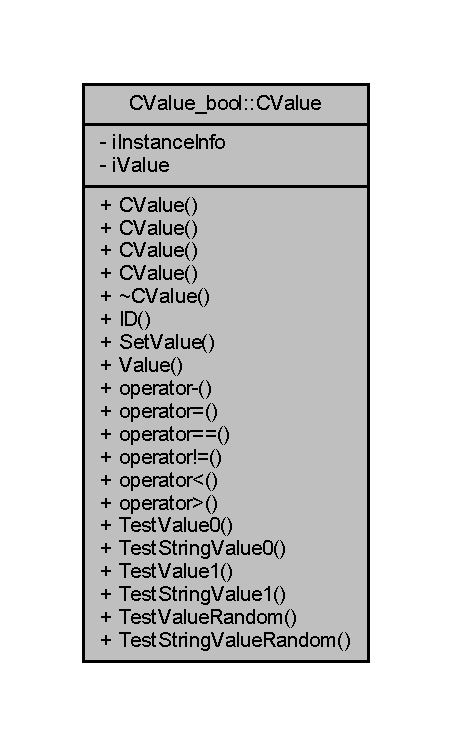
\includegraphics[width=217pt]{class_c_value__bool_1_1_c_value__coll__graph}
\end{center}
\end{figure}
\subsection*{Public Member Functions}
\begin{DoxyCompactItemize}
\item 
\hyperlink{class_c_value__bool_1_1_c_value_a16e53bf59cc84c4cf0527e08f1f2fde4}{C\+Value} ()
\begin{DoxyCompactList}\small\item\em Implicit c\textquotesingle{}tor. \end{DoxyCompactList}\item 
\hyperlink{class_c_value__bool_1_1_c_value_af0fe821e94aae8cbef4e3b427748ddd8}{C\+Value} (const bool a\+Value)
\begin{DoxyCompactList}\small\item\em Conversion c\textquotesingle{}tor. \end{DoxyCompactList}\item 
\hyperlink{class_c_value__bool_1_1_c_value_abc234c189a9447eb7859f8c7731122e1}{C\+Value} (const \hyperlink{class_c_value__bool_1_1_c_value}{C\+Value} \&a\+Value)
\begin{DoxyCompactList}\small\item\em Copy c\textquotesingle{}tor. \end{DoxyCompactList}\item 
\hyperlink{class_c_value__bool_1_1_c_value_a8883e123d12aed4cd3ca24db42ea0049}{C\+Value} (const char $\ast$a\+Str)
\begin{DoxyCompactList}\small\item\em String conversion c\textquotesingle{}tor. \end{DoxyCompactList}\item 
virtual \hyperlink{class_c_value__bool_1_1_c_value_acdc5cb2d30dedc5f34d586e2560eea79}{$\sim$\+C\+Value} () noexcept(false)
\begin{DoxyCompactList}\small\item\em Virtual d\textquotesingle{}tor. \end{DoxyCompactList}\item 
size\+\_\+t \hyperlink{class_c_value__bool_1_1_c_value_a028335ed71781b92b96dfb51e1118eda}{ID} () const
\begin{DoxyCompactList}\small\item\em ID getter. \end{DoxyCompactList}\item 
void \hyperlink{class_c_value__bool_1_1_c_value_ab39b87a635a8d3651fa9bd1d06669d82}{Set\+Value} (const bool a\+Value)
\begin{DoxyCompactList}\small\item\em Value setter. \end{DoxyCompactList}\item 
bool \hyperlink{class_c_value__bool_1_1_c_value_a78e9392ca4d446ed32a83ad5a89b075d}{Value} () const
\begin{DoxyCompactList}\small\item\em Value getter. \end{DoxyCompactList}\item 
\hyperlink{class_c_value__bool_1_1_c_value}{C\+Value} \hyperlink{class_c_value__bool_1_1_c_value_a6fe95b37e5928d4ea12b8bfcdafc0027}{operator-\/} () const
\begin{DoxyCompactList}\small\item\em Complement operator. \end{DoxyCompactList}\item 
\hyperlink{class_c_value__bool_1_1_c_value}{C\+Value} \& \hyperlink{class_c_value__bool_1_1_c_value_ace6035c9ce867111440ef2c9c336852f}{operator=} (const \hyperlink{class_c_value__bool_1_1_c_value}{C\+Value} \&a\+Value)
\begin{DoxyCompactList}\small\item\em Assigment operator. \end{DoxyCompactList}\item 
bool \hyperlink{class_c_value__bool_1_1_c_value_aa0ef6517b9d79e30e198d970ebb121c9}{operator==} (const \hyperlink{class_c_value__bool_1_1_c_value}{C\+Value} \&a\+Value) const
\begin{DoxyCompactList}\small\item\em Comparing by Value operator. \end{DoxyCompactList}\item 
bool \hyperlink{class_c_value__bool_1_1_c_value_ad77db9403e1e923b324aa919108609e6}{operator!=} (const \hyperlink{class_c_value__bool_1_1_c_value}{C\+Value} \&a\+Value) const
\begin{DoxyCompactList}\small\item\em Comparing by Value operator. \end{DoxyCompactList}\item 
bool \hyperlink{class_c_value__bool_1_1_c_value_ac23e4f8e65e397ae113818bf679f438f}{operator$<$} (const \hyperlink{class_c_value__bool_1_1_c_value}{C\+Value} \&a\+Value) const
\begin{DoxyCompactList}\small\item\em Comparing by Value operator. \end{DoxyCompactList}\item 
bool \hyperlink{class_c_value__bool_1_1_c_value_ac1f4a9bb08a0538073455f303f853c12}{operator$>$} (const \hyperlink{class_c_value__bool_1_1_c_value}{C\+Value} \&a\+Value) const
\begin{DoxyCompactList}\small\item\em Comparing by Value operator. \end{DoxyCompactList}\end{DoxyCompactItemize}
\subsection*{Static Public Member Functions}
\begin{DoxyCompactItemize}
\item 
static bool \hyperlink{class_c_value__bool_1_1_c_value_a6a39f590a87bb4be8f707c032ca2b32b}{Test\+Value0} ()
\begin{DoxyCompactList}\small\item\em First test value. \end{DoxyCompactList}\item 
static const char $\ast$ \hyperlink{class_c_value__bool_1_1_c_value_ae327d8276f5f4c75705c7413d5942ea0}{Test\+String\+Value0} ()
\begin{DoxyCompactList}\small\item\em First test string value. \end{DoxyCompactList}\item 
static bool \hyperlink{class_c_value__bool_1_1_c_value_a73b53a394f0b2ebeebeecad0610949b8}{Test\+Value1} ()
\begin{DoxyCompactList}\small\item\em Second test value. \end{DoxyCompactList}\item 
static const char $\ast$ \hyperlink{class_c_value__bool_1_1_c_value_a2d82d7f212af01b330e3bc3514961a5a}{Test\+String\+Value1} ()
\begin{DoxyCompactList}\small\item\em Second test string value. \end{DoxyCompactList}\item 
static bool \hyperlink{class_c_value__bool_1_1_c_value_a5583585b33adfb3b27d9b49ad1a7cc3a}{Test\+Value\+Random} ()
\begin{DoxyCompactList}\small\item\em Random test value. \end{DoxyCompactList}\item 
static const char $\ast$ \hyperlink{class_c_value__bool_1_1_c_value_a84d39c7918bfb7876640a8b64e2e8c95}{Test\+String\+Value\+Random} ()
\begin{DoxyCompactList}\small\item\em Random test string value. \end{DoxyCompactList}\end{DoxyCompactItemize}
\subsection*{Private Attributes}
\begin{DoxyCompactItemize}
\item 
Class\+Info$<$ \hyperlink{class_c_value__bool_1_1_c_value}{C\+Value} $>$ \hyperlink{class_c_value__bool_1_1_c_value_a5e9470a5efc80373b5cc943f25d1a803}{i\+Instance\+Info}
\begin{DoxyCompactList}\small\item\em Instance of the class info for usage statistics. \end{DoxyCompactList}\item 
bool \hyperlink{class_c_value__bool_1_1_c_value_a2a05b9efee1e0497a631a39b0146b776}{i\+Value}
\begin{DoxyCompactList}\small\item\em Encapsulated {\ttfamily bool} value. \end{DoxyCompactList}\end{DoxyCompactItemize}
\subsection*{Friends}
\begin{DoxyCompactItemize}
\item 
std\+::ostream \& \hyperlink{class_c_value__bool_1_1_c_value_a3d28097fae6bdd5a8146d9ab90f8b62f}{operator$<$$<$} (std\+::ostream \&a\+O\+Stream, const \hyperlink{class_c_value__bool_1_1_c_value}{C\+Value} \&a\+Value)
\begin{DoxyCompactList}\small\item\em Output to the stream operator. ({\itshape serialization}) \end{DoxyCompactList}\item 
std\+::istream \& \hyperlink{class_c_value__bool_1_1_c_value_aba05045ca890e398c1211784aebbc9ed}{operator$>$$>$} (std\+::istream \&a\+I\+Stream, \hyperlink{class_c_value__bool_1_1_c_value}{C\+Value} \&a\+Value)
\begin{DoxyCompactList}\small\item\em Input from the stream operator. ({\itshape deserialization}) \end{DoxyCompactList}\end{DoxyCompactItemize}


\subsection{Detailed Description}
\hyperlink{class_c_value__bool_1_1_c_value}{C\+Value} class ({\ttfamily bool} variant) 

Definition of \hyperlink{class_c_value__bool_1_1_c_value}{C\+Value} class ({\ttfamily bool} variant). There is defined all common methods and attributes. 

Definition at line 27 of file C\+Value\+\_\+bool.\+h.



\subsection{Constructor \& Destructor Documentation}
\mbox{\Hypertarget{class_c_value__bool_1_1_c_value_a16e53bf59cc84c4cf0527e08f1f2fde4}\label{class_c_value__bool_1_1_c_value_a16e53bf59cc84c4cf0527e08f1f2fde4}} 
\index{C\+Value\+\_\+bool\+::\+C\+Value@{C\+Value\+\_\+bool\+::\+C\+Value}!C\+Value@{C\+Value}}
\index{C\+Value@{C\+Value}!C\+Value\+\_\+bool\+::\+C\+Value@{C\+Value\+\_\+bool\+::\+C\+Value}}
\subsubsection{\texorpdfstring{C\+Value()}{CValue()}\hspace{0.1cm}{\footnotesize\ttfamily [1/4]}}
{\footnotesize\ttfamily C\+Value\+\_\+bool\+::\+C\+Value\+::\+C\+Value (\begin{DoxyParamCaption}{ }\end{DoxyParamCaption})\hspace{0.3cm}{\ttfamily [inline]}}



Implicit c\textquotesingle{}tor. 

Value attributes is set to {\ttfamily false}. 

Definition at line 37 of file C\+Value\+\_\+bool.\+h.

\mbox{\Hypertarget{class_c_value__bool_1_1_c_value_af0fe821e94aae8cbef4e3b427748ddd8}\label{class_c_value__bool_1_1_c_value_af0fe821e94aae8cbef4e3b427748ddd8}} 
\index{C\+Value\+\_\+bool\+::\+C\+Value@{C\+Value\+\_\+bool\+::\+C\+Value}!C\+Value@{C\+Value}}
\index{C\+Value@{C\+Value}!C\+Value\+\_\+bool\+::\+C\+Value@{C\+Value\+\_\+bool\+::\+C\+Value}}
\subsubsection{\texorpdfstring{C\+Value()}{CValue()}\hspace{0.1cm}{\footnotesize\ttfamily [2/4]}}
{\footnotesize\ttfamily C\+Value\+\_\+bool\+::\+C\+Value\+::\+C\+Value (\begin{DoxyParamCaption}\item[{const bool}]{a\+Value }\end{DoxyParamCaption})\hspace{0.3cm}{\ttfamily [inline]}, {\ttfamily [explicit]}}



Conversion c\textquotesingle{}tor. 

Pointer attributes are initialised to the {\ttfamily this} value. 
\begin{DoxyParams}[1]{Parameters}
\mbox{\tt in}  & {\em a\+Value} & New encapsulated {\ttfamily bool} Value \\
\hline
\end{DoxyParams}


Definition at line 44 of file C\+Value\+\_\+bool.\+h.

\mbox{\Hypertarget{class_c_value__bool_1_1_c_value_abc234c189a9447eb7859f8c7731122e1}\label{class_c_value__bool_1_1_c_value_abc234c189a9447eb7859f8c7731122e1}} 
\index{C\+Value\+\_\+bool\+::\+C\+Value@{C\+Value\+\_\+bool\+::\+C\+Value}!C\+Value@{C\+Value}}
\index{C\+Value@{C\+Value}!C\+Value\+\_\+bool\+::\+C\+Value@{C\+Value\+\_\+bool\+::\+C\+Value}}
\subsubsection{\texorpdfstring{C\+Value()}{CValue()}\hspace{0.1cm}{\footnotesize\ttfamily [3/4]}}
{\footnotesize\ttfamily C\+Value\+\_\+bool\+::\+C\+Value\+::\+C\+Value (\begin{DoxyParamCaption}\item[{const \hyperlink{class_c_value__bool_1_1_c_value}{C\+Value} \&}]{a\+Value }\end{DoxyParamCaption})\hspace{0.3cm}{\ttfamily [inline]}}



Copy c\textquotesingle{}tor. 

Create new instance by copying only {\ttfamily i\+Value} parameter. 
\begin{DoxyParams}[1]{Parameters}
\mbox{\tt in}  & {\em a\+Value} & Original instance for copying \\
\hline
\end{DoxyParams}


Definition at line 51 of file C\+Value\+\_\+bool.\+h.

\mbox{\Hypertarget{class_c_value__bool_1_1_c_value_a8883e123d12aed4cd3ca24db42ea0049}\label{class_c_value__bool_1_1_c_value_a8883e123d12aed4cd3ca24db42ea0049}} 
\index{C\+Value\+\_\+bool\+::\+C\+Value@{C\+Value\+\_\+bool\+::\+C\+Value}!C\+Value@{C\+Value}}
\index{C\+Value@{C\+Value}!C\+Value\+\_\+bool\+::\+C\+Value@{C\+Value\+\_\+bool\+::\+C\+Value}}
\subsubsection{\texorpdfstring{C\+Value()}{CValue()}\hspace{0.1cm}{\footnotesize\ttfamily [4/4]}}
{\footnotesize\ttfamily C\+Value\+\_\+bool\+::\+C\+Value\+::\+C\+Value (\begin{DoxyParamCaption}\item[{const char $\ast$}]{a\+Str }\end{DoxyParamCaption})\hspace{0.3cm}{\ttfamily [inline]}, {\ttfamily [explicit]}}



String conversion c\textquotesingle{}tor. 

Create new instance from Value in the string. Pointer attributes are initialised to the {\ttfamily this} value. 
\begin{DoxyParams}[1]{Parameters}
\mbox{\tt in}  & {\em a\+Str} & Plain C string with value \char`\"{}0\char`\"{} or \char`\"{}1\char`\"{} \\
\hline
\end{DoxyParams}


Definition at line 58 of file C\+Value\+\_\+bool.\+h.

\mbox{\Hypertarget{class_c_value__bool_1_1_c_value_acdc5cb2d30dedc5f34d586e2560eea79}\label{class_c_value__bool_1_1_c_value_acdc5cb2d30dedc5f34d586e2560eea79}} 
\index{C\+Value\+\_\+bool\+::\+C\+Value@{C\+Value\+\_\+bool\+::\+C\+Value}!````~C\+Value@{$\sim$\+C\+Value}}
\index{````~C\+Value@{$\sim$\+C\+Value}!C\+Value\+\_\+bool\+::\+C\+Value@{C\+Value\+\_\+bool\+::\+C\+Value}}
\subsubsection{\texorpdfstring{$\sim$\+C\+Value()}{~CValue()}}
{\footnotesize\ttfamily virtual C\+Value\+\_\+bool\+::\+C\+Value\+::$\sim$\+C\+Value (\begin{DoxyParamCaption}{ }\end{DoxyParamCaption})\hspace{0.3cm}{\ttfamily [inline]}, {\ttfamily [virtual]}, {\ttfamily [noexcept]}}



Virtual d\textquotesingle{}tor. 



Definition at line 64 of file C\+Value\+\_\+bool.\+h.



\subsection{Member Function Documentation}
\mbox{\Hypertarget{class_c_value__bool_1_1_c_value_a028335ed71781b92b96dfb51e1118eda}\label{class_c_value__bool_1_1_c_value_a028335ed71781b92b96dfb51e1118eda}} 
\index{C\+Value\+\_\+bool\+::\+C\+Value@{C\+Value\+\_\+bool\+::\+C\+Value}!ID@{ID}}
\index{ID@{ID}!C\+Value\+\_\+bool\+::\+C\+Value@{C\+Value\+\_\+bool\+::\+C\+Value}}
\subsubsection{\texorpdfstring{I\+D()}{ID()}}
{\footnotesize\ttfamily size\+\_\+t C\+Value\+\_\+bool\+::\+C\+Value\+::\+ID (\begin{DoxyParamCaption}{ }\end{DoxyParamCaption}) const\hspace{0.3cm}{\ttfamily [inline]}}



ID getter. 

\begin{DoxyReturn}{Returns}
Unique instance ID 
\end{DoxyReturn}


Definition at line 71 of file C\+Value\+\_\+bool.\+h.

\mbox{\Hypertarget{class_c_value__bool_1_1_c_value_ad77db9403e1e923b324aa919108609e6}\label{class_c_value__bool_1_1_c_value_ad77db9403e1e923b324aa919108609e6}} 
\index{C\+Value\+\_\+bool\+::\+C\+Value@{C\+Value\+\_\+bool\+::\+C\+Value}!operator"!=@{operator"!=}}
\index{operator"!=@{operator"!=}!C\+Value\+\_\+bool\+::\+C\+Value@{C\+Value\+\_\+bool\+::\+C\+Value}}
\subsubsection{\texorpdfstring{operator"!=()}{operator!=()}}
{\footnotesize\ttfamily bool C\+Value\+\_\+bool\+::\+C\+Value\+::operator!= (\begin{DoxyParamCaption}\item[{const \hyperlink{class_c_value__bool_1_1_c_value}{C\+Value} \&}]{a\+Value }\end{DoxyParamCaption}) const\hspace{0.3cm}{\ttfamily [inline]}}



Comparing by Value operator. 

\begin{DoxyReturn}{Returns}
Return {\ttfamily bool} result of comparation 
\end{DoxyReturn}


Definition at line 109 of file C\+Value\+\_\+bool.\+h.

\mbox{\Hypertarget{class_c_value__bool_1_1_c_value_a6fe95b37e5928d4ea12b8bfcdafc0027}\label{class_c_value__bool_1_1_c_value_a6fe95b37e5928d4ea12b8bfcdafc0027}} 
\index{C\+Value\+\_\+bool\+::\+C\+Value@{C\+Value\+\_\+bool\+::\+C\+Value}!operator-\/@{operator-\/}}
\index{operator-\/@{operator-\/}!C\+Value\+\_\+bool\+::\+C\+Value@{C\+Value\+\_\+bool\+::\+C\+Value}}
\subsubsection{\texorpdfstring{operator-\/()}{operator-()}}
{\footnotesize\ttfamily \hyperlink{class_c_value__bool_1_1_c_value}{C\+Value} C\+Value\+\_\+bool\+::\+C\+Value\+::operator-\/ (\begin{DoxyParamCaption}{ }\end{DoxyParamCaption}) const\hspace{0.3cm}{\ttfamily [inline]}}



Complement operator. 

\begin{DoxyReturn}{Returns}
\hyperlink{class_c_value__bool_1_1_c_value}{C\+Value} instance with complemented attribute Value. 
\end{DoxyReturn}


Definition at line 91 of file C\+Value\+\_\+bool.\+h.

\mbox{\Hypertarget{class_c_value__bool_1_1_c_value_ac23e4f8e65e397ae113818bf679f438f}\label{class_c_value__bool_1_1_c_value_ac23e4f8e65e397ae113818bf679f438f}} 
\index{C\+Value\+\_\+bool\+::\+C\+Value@{C\+Value\+\_\+bool\+::\+C\+Value}!operator$<$@{operator$<$}}
\index{operator$<$@{operator$<$}!C\+Value\+\_\+bool\+::\+C\+Value@{C\+Value\+\_\+bool\+::\+C\+Value}}
\subsubsection{\texorpdfstring{operator$<$()}{operator<()}}
{\footnotesize\ttfamily bool C\+Value\+\_\+bool\+::\+C\+Value\+::operator$<$ (\begin{DoxyParamCaption}\item[{const \hyperlink{class_c_value__bool_1_1_c_value}{C\+Value} \&}]{a\+Value }\end{DoxyParamCaption}) const\hspace{0.3cm}{\ttfamily [inline]}}



Comparing by Value operator. 

\begin{DoxyReturn}{Returns}
Return {\ttfamily bool} result of comparation 
\end{DoxyReturn}


Definition at line 115 of file C\+Value\+\_\+bool.\+h.

\mbox{\Hypertarget{class_c_value__bool_1_1_c_value_ace6035c9ce867111440ef2c9c336852f}\label{class_c_value__bool_1_1_c_value_ace6035c9ce867111440ef2c9c336852f}} 
\index{C\+Value\+\_\+bool\+::\+C\+Value@{C\+Value\+\_\+bool\+::\+C\+Value}!operator=@{operator=}}
\index{operator=@{operator=}!C\+Value\+\_\+bool\+::\+C\+Value@{C\+Value\+\_\+bool\+::\+C\+Value}}
\subsubsection{\texorpdfstring{operator=()}{operator=()}}
{\footnotesize\ttfamily \hyperlink{class_c_value__bool_1_1_c_value}{C\+Value}\& C\+Value\+\_\+bool\+::\+C\+Value\+::operator= (\begin{DoxyParamCaption}\item[{const \hyperlink{class_c_value__bool_1_1_c_value}{C\+Value} \&}]{a\+Value }\end{DoxyParamCaption})\hspace{0.3cm}{\ttfamily [inline]}}



Assigment operator. 

\begin{DoxyReturn}{Returns}
\hyperlink{class_c_value__bool_1_1_c_value}{C\+Value} instance with copied attribute Value. 
\end{DoxyReturn}


Definition at line 97 of file C\+Value\+\_\+bool.\+h.

\mbox{\Hypertarget{class_c_value__bool_1_1_c_value_aa0ef6517b9d79e30e198d970ebb121c9}\label{class_c_value__bool_1_1_c_value_aa0ef6517b9d79e30e198d970ebb121c9}} 
\index{C\+Value\+\_\+bool\+::\+C\+Value@{C\+Value\+\_\+bool\+::\+C\+Value}!operator==@{operator==}}
\index{operator==@{operator==}!C\+Value\+\_\+bool\+::\+C\+Value@{C\+Value\+\_\+bool\+::\+C\+Value}}
\subsubsection{\texorpdfstring{operator==()}{operator==()}}
{\footnotesize\ttfamily bool C\+Value\+\_\+bool\+::\+C\+Value\+::operator== (\begin{DoxyParamCaption}\item[{const \hyperlink{class_c_value__bool_1_1_c_value}{C\+Value} \&}]{a\+Value }\end{DoxyParamCaption}) const\hspace{0.3cm}{\ttfamily [inline]}}



Comparing by Value operator. 

\begin{DoxyReturn}{Returns}
Return {\ttfamily bool} result of comparation 
\end{DoxyReturn}


Definition at line 103 of file C\+Value\+\_\+bool.\+h.

\mbox{\Hypertarget{class_c_value__bool_1_1_c_value_ac1f4a9bb08a0538073455f303f853c12}\label{class_c_value__bool_1_1_c_value_ac1f4a9bb08a0538073455f303f853c12}} 
\index{C\+Value\+\_\+bool\+::\+C\+Value@{C\+Value\+\_\+bool\+::\+C\+Value}!operator$>$@{operator$>$}}
\index{operator$>$@{operator$>$}!C\+Value\+\_\+bool\+::\+C\+Value@{C\+Value\+\_\+bool\+::\+C\+Value}}
\subsubsection{\texorpdfstring{operator$>$()}{operator>()}}
{\footnotesize\ttfamily bool C\+Value\+\_\+bool\+::\+C\+Value\+::operator$>$ (\begin{DoxyParamCaption}\item[{const \hyperlink{class_c_value__bool_1_1_c_value}{C\+Value} \&}]{a\+Value }\end{DoxyParamCaption}) const\hspace{0.3cm}{\ttfamily [inline]}}



Comparing by Value operator. 

\begin{DoxyReturn}{Returns}
Return {\ttfamily bool} result of comparation 
\end{DoxyReturn}


Definition at line 121 of file C\+Value\+\_\+bool.\+h.

\mbox{\Hypertarget{class_c_value__bool_1_1_c_value_ab39b87a635a8d3651fa9bd1d06669d82}\label{class_c_value__bool_1_1_c_value_ab39b87a635a8d3651fa9bd1d06669d82}} 
\index{C\+Value\+\_\+bool\+::\+C\+Value@{C\+Value\+\_\+bool\+::\+C\+Value}!Set\+Value@{Set\+Value}}
\index{Set\+Value@{Set\+Value}!C\+Value\+\_\+bool\+::\+C\+Value@{C\+Value\+\_\+bool\+::\+C\+Value}}
\subsubsection{\texorpdfstring{Set\+Value()}{SetValue()}}
{\footnotesize\ttfamily void C\+Value\+\_\+bool\+::\+C\+Value\+::\+Set\+Value (\begin{DoxyParamCaption}\item[{const bool}]{a\+Value }\end{DoxyParamCaption})\hspace{0.3cm}{\ttfamily [inline]}}



Value setter. 


\begin{DoxyParams}[1]{Parameters}
\mbox{\tt in}  & {\em a\+Value} & New Value \\
\hline
\end{DoxyParams}


Definition at line 78 of file C\+Value\+\_\+bool.\+h.

\mbox{\Hypertarget{class_c_value__bool_1_1_c_value_ae327d8276f5f4c75705c7413d5942ea0}\label{class_c_value__bool_1_1_c_value_ae327d8276f5f4c75705c7413d5942ea0}} 
\index{C\+Value\+\_\+bool\+::\+C\+Value@{C\+Value\+\_\+bool\+::\+C\+Value}!Test\+String\+Value0@{Test\+String\+Value0}}
\index{Test\+String\+Value0@{Test\+String\+Value0}!C\+Value\+\_\+bool\+::\+C\+Value@{C\+Value\+\_\+bool\+::\+C\+Value}}
\subsubsection{\texorpdfstring{Test\+String\+Value0()}{TestStringValue0()}}
{\footnotesize\ttfamily static const char$\ast$ C\+Value\+\_\+bool\+::\+C\+Value\+::\+Test\+String\+Value0 (\begin{DoxyParamCaption}{ }\end{DoxyParamCaption})\hspace{0.3cm}{\ttfamily [inline]}, {\ttfamily [static]}}



First test string value. 

\begin{DoxyReturn}{Returns}
Return string with {\ttfamily bool} value ({\ttfamily false}) 
\end{DoxyReturn}
\begin{DoxyNote}{Note}
Useful for automated testing of \hyperlink{class_c_value__bool_1_1_c_value}{C\+Value} functionality 
\end{DoxyNote}


Definition at line 164 of file C\+Value\+\_\+bool.\+h.

\mbox{\Hypertarget{class_c_value__bool_1_1_c_value_a2d82d7f212af01b330e3bc3514961a5a}\label{class_c_value__bool_1_1_c_value_a2d82d7f212af01b330e3bc3514961a5a}} 
\index{C\+Value\+\_\+bool\+::\+C\+Value@{C\+Value\+\_\+bool\+::\+C\+Value}!Test\+String\+Value1@{Test\+String\+Value1}}
\index{Test\+String\+Value1@{Test\+String\+Value1}!C\+Value\+\_\+bool\+::\+C\+Value@{C\+Value\+\_\+bool\+::\+C\+Value}}
\subsubsection{\texorpdfstring{Test\+String\+Value1()}{TestStringValue1()}}
{\footnotesize\ttfamily static const char$\ast$ C\+Value\+\_\+bool\+::\+C\+Value\+::\+Test\+String\+Value1 (\begin{DoxyParamCaption}{ }\end{DoxyParamCaption})\hspace{0.3cm}{\ttfamily [inline]}, {\ttfamily [static]}}



Second test string value. 

\begin{DoxyReturn}{Returns}
Return string with {\ttfamily bool} value ({\ttfamily true}) 
\end{DoxyReturn}
\begin{DoxyNote}{Note}
Useful for automated testing of \hyperlink{class_c_value__bool_1_1_c_value}{C\+Value} functionality 
\end{DoxyNote}


Definition at line 178 of file C\+Value\+\_\+bool.\+h.

\mbox{\Hypertarget{class_c_value__bool_1_1_c_value_a84d39c7918bfb7876640a8b64e2e8c95}\label{class_c_value__bool_1_1_c_value_a84d39c7918bfb7876640a8b64e2e8c95}} 
\index{C\+Value\+\_\+bool\+::\+C\+Value@{C\+Value\+\_\+bool\+::\+C\+Value}!Test\+String\+Value\+Random@{Test\+String\+Value\+Random}}
\index{Test\+String\+Value\+Random@{Test\+String\+Value\+Random}!C\+Value\+\_\+bool\+::\+C\+Value@{C\+Value\+\_\+bool\+::\+C\+Value}}
\subsubsection{\texorpdfstring{Test\+String\+Value\+Random()}{TestStringValueRandom()}}
{\footnotesize\ttfamily static const char$\ast$ C\+Value\+\_\+bool\+::\+C\+Value\+::\+Test\+String\+Value\+Random (\begin{DoxyParamCaption}{ }\end{DoxyParamCaption})\hspace{0.3cm}{\ttfamily [inline]}, {\ttfamily [static]}}



Random test string value. 

\begin{DoxyReturn}{Returns}
Return string with random {\ttfamily bool} value 
\end{DoxyReturn}
\begin{DoxyNote}{Note}
Useful for automated testing of \hyperlink{class_c_value__bool_1_1_c_value}{C\+Value} functionality 
\end{DoxyNote}


Definition at line 192 of file C\+Value\+\_\+bool.\+h.

\mbox{\Hypertarget{class_c_value__bool_1_1_c_value_a6a39f590a87bb4be8f707c032ca2b32b}\label{class_c_value__bool_1_1_c_value_a6a39f590a87bb4be8f707c032ca2b32b}} 
\index{C\+Value\+\_\+bool\+::\+C\+Value@{C\+Value\+\_\+bool\+::\+C\+Value}!Test\+Value0@{Test\+Value0}}
\index{Test\+Value0@{Test\+Value0}!C\+Value\+\_\+bool\+::\+C\+Value@{C\+Value\+\_\+bool\+::\+C\+Value}}
\subsubsection{\texorpdfstring{Test\+Value0()}{TestValue0()}}
{\footnotesize\ttfamily static bool C\+Value\+\_\+bool\+::\+C\+Value\+::\+Test\+Value0 (\begin{DoxyParamCaption}{ }\end{DoxyParamCaption})\hspace{0.3cm}{\ttfamily [inline]}, {\ttfamily [static]}}



First test value. 

\begin{DoxyReturn}{Returns}
Return {\ttfamily bool} value ({\ttfamily false}) 
\end{DoxyReturn}
\begin{DoxyNote}{Note}
Useful for automated testing of \hyperlink{class_c_value__bool_1_1_c_value}{C\+Value} functionality 
\end{DoxyNote}


Definition at line 157 of file C\+Value\+\_\+bool.\+h.

\mbox{\Hypertarget{class_c_value__bool_1_1_c_value_a73b53a394f0b2ebeebeecad0610949b8}\label{class_c_value__bool_1_1_c_value_a73b53a394f0b2ebeebeecad0610949b8}} 
\index{C\+Value\+\_\+bool\+::\+C\+Value@{C\+Value\+\_\+bool\+::\+C\+Value}!Test\+Value1@{Test\+Value1}}
\index{Test\+Value1@{Test\+Value1}!C\+Value\+\_\+bool\+::\+C\+Value@{C\+Value\+\_\+bool\+::\+C\+Value}}
\subsubsection{\texorpdfstring{Test\+Value1()}{TestValue1()}}
{\footnotesize\ttfamily static bool C\+Value\+\_\+bool\+::\+C\+Value\+::\+Test\+Value1 (\begin{DoxyParamCaption}{ }\end{DoxyParamCaption})\hspace{0.3cm}{\ttfamily [inline]}, {\ttfamily [static]}}



Second test value. 

\begin{DoxyReturn}{Returns}
Return {\ttfamily bool} value ({\ttfamily true}) 
\end{DoxyReturn}
\begin{DoxyNote}{Note}
Useful for automated testing of \hyperlink{class_c_value__bool_1_1_c_value}{C\+Value} functionality 
\end{DoxyNote}


Definition at line 171 of file C\+Value\+\_\+bool.\+h.

\mbox{\Hypertarget{class_c_value__bool_1_1_c_value_a5583585b33adfb3b27d9b49ad1a7cc3a}\label{class_c_value__bool_1_1_c_value_a5583585b33adfb3b27d9b49ad1a7cc3a}} 
\index{C\+Value\+\_\+bool\+::\+C\+Value@{C\+Value\+\_\+bool\+::\+C\+Value}!Test\+Value\+Random@{Test\+Value\+Random}}
\index{Test\+Value\+Random@{Test\+Value\+Random}!C\+Value\+\_\+bool\+::\+C\+Value@{C\+Value\+\_\+bool\+::\+C\+Value}}
\subsubsection{\texorpdfstring{Test\+Value\+Random()}{TestValueRandom()}}
{\footnotesize\ttfamily static bool C\+Value\+\_\+bool\+::\+C\+Value\+::\+Test\+Value\+Random (\begin{DoxyParamCaption}{ }\end{DoxyParamCaption})\hspace{0.3cm}{\ttfamily [inline]}, {\ttfamily [static]}}



Random test value. 

\begin{DoxyReturn}{Returns}
Return random {\ttfamily bool} value 
\end{DoxyReturn}
\begin{DoxyNote}{Note}
Useful for automated testing of \hyperlink{class_c_value__bool_1_1_c_value}{C\+Value} functionality 
\end{DoxyNote}


Definition at line 185 of file C\+Value\+\_\+bool.\+h.

\mbox{\Hypertarget{class_c_value__bool_1_1_c_value_a78e9392ca4d446ed32a83ad5a89b075d}\label{class_c_value__bool_1_1_c_value_a78e9392ca4d446ed32a83ad5a89b075d}} 
\index{C\+Value\+\_\+bool\+::\+C\+Value@{C\+Value\+\_\+bool\+::\+C\+Value}!Value@{Value}}
\index{Value@{Value}!C\+Value\+\_\+bool\+::\+C\+Value@{C\+Value\+\_\+bool\+::\+C\+Value}}
\subsubsection{\texorpdfstring{Value()}{Value()}}
{\footnotesize\ttfamily bool C\+Value\+\_\+bool\+::\+C\+Value\+::\+Value (\begin{DoxyParamCaption}{ }\end{DoxyParamCaption}) const\hspace{0.3cm}{\ttfamily [inline]}}



Value getter. 

\begin{DoxyReturn}{Returns}
Actual {\ttfamily bool} {\ttfamily Value} 
\end{DoxyReturn}


Definition at line 84 of file C\+Value\+\_\+bool.\+h.



\subsection{Friends And Related Function Documentation}
\mbox{\Hypertarget{class_c_value__bool_1_1_c_value_a3d28097fae6bdd5a8146d9ab90f8b62f}\label{class_c_value__bool_1_1_c_value_a3d28097fae6bdd5a8146d9ab90f8b62f}} 
\index{C\+Value\+\_\+bool\+::\+C\+Value@{C\+Value\+\_\+bool\+::\+C\+Value}!operator$<$$<$@{operator$<$$<$}}
\index{operator$<$$<$@{operator$<$$<$}!C\+Value\+\_\+bool\+::\+C\+Value@{C\+Value\+\_\+bool\+::\+C\+Value}}
\subsubsection{\texorpdfstring{operator$<$$<$}{operator<<}}
{\footnotesize\ttfamily std\+::ostream\& operator$<$$<$ (\begin{DoxyParamCaption}\item[{std\+::ostream \&}]{a\+O\+Stream,  }\item[{const \hyperlink{class_c_value__bool_1_1_c_value}{C\+Value} \&}]{a\+Value }\end{DoxyParamCaption})\hspace{0.3cm}{\ttfamily [friend]}}



Output to the stream operator. ({\itshape serialization}) 


\begin{DoxyParams}[1]{Parameters}
\mbox{\tt in}  & {\em a\+O\+Stream} & Output stream \\
\hline
\mbox{\tt in}  & {\em a\+Value} & Serialized instantion of \hyperlink{class_c_value__bool_1_1_c_value}{C\+Value} \\
\hline
\end{DoxyParams}
\begin{DoxyReturn}{Returns}
Return {\ttfamily std\+::ostream} with serialized Value 
\end{DoxyReturn}


Definition at line 129 of file C\+Value\+\_\+bool.\+h.

\mbox{\Hypertarget{class_c_value__bool_1_1_c_value_aba05045ca890e398c1211784aebbc9ed}\label{class_c_value__bool_1_1_c_value_aba05045ca890e398c1211784aebbc9ed}} 
\index{C\+Value\+\_\+bool\+::\+C\+Value@{C\+Value\+\_\+bool\+::\+C\+Value}!operator$>$$>$@{operator$>$$>$}}
\index{operator$>$$>$@{operator$>$$>$}!C\+Value\+\_\+bool\+::\+C\+Value@{C\+Value\+\_\+bool\+::\+C\+Value}}
\subsubsection{\texorpdfstring{operator$>$$>$}{operator>>}}
{\footnotesize\ttfamily std\+::istream\& operator$>$$>$ (\begin{DoxyParamCaption}\item[{std\+::istream \&}]{a\+I\+Stream,  }\item[{\hyperlink{class_c_value__bool_1_1_c_value}{C\+Value} \&}]{a\+Value }\end{DoxyParamCaption})\hspace{0.3cm}{\ttfamily [friend]}}



Input from the stream operator. ({\itshape deserialization}) 


\begin{DoxyParams}[1]{Parameters}
\mbox{\tt in}  & {\em a\+I\+Stream} & Input stream \\
\hline
\mbox{\tt out}  & {\em a\+Value} & Place for deserialized instantion of \hyperlink{class_c_value__bool_1_1_c_value}{C\+Value} \\
\hline
\end{DoxyParams}
\begin{DoxyReturn}{Returns}
Return rest of {\ttfamily std\+::istream} 
\end{DoxyReturn}


Definition at line 142 of file C\+Value\+\_\+bool.\+h.



\subsection{Member Data Documentation}
\mbox{\Hypertarget{class_c_value__bool_1_1_c_value_a5e9470a5efc80373b5cc943f25d1a803}\label{class_c_value__bool_1_1_c_value_a5e9470a5efc80373b5cc943f25d1a803}} 
\index{C\+Value\+\_\+bool\+::\+C\+Value@{C\+Value\+\_\+bool\+::\+C\+Value}!i\+Instance\+Info@{i\+Instance\+Info}}
\index{i\+Instance\+Info@{i\+Instance\+Info}!C\+Value\+\_\+bool\+::\+C\+Value@{C\+Value\+\_\+bool\+::\+C\+Value}}
\subsubsection{\texorpdfstring{i\+Instance\+Info}{iInstanceInfo}}
{\footnotesize\ttfamily Class\+Info$<$\hyperlink{class_c_value__bool_1_1_c_value}{C\+Value}$>$ C\+Value\+\_\+bool\+::\+C\+Value\+::i\+Instance\+Info\hspace{0.3cm}{\ttfamily [private]}}



Instance of the class info for usage statistics. 



Definition at line 29 of file C\+Value\+\_\+bool.\+h.

\mbox{\Hypertarget{class_c_value__bool_1_1_c_value_a2a05b9efee1e0497a631a39b0146b776}\label{class_c_value__bool_1_1_c_value_a2a05b9efee1e0497a631a39b0146b776}} 
\index{C\+Value\+\_\+bool\+::\+C\+Value@{C\+Value\+\_\+bool\+::\+C\+Value}!i\+Value@{i\+Value}}
\index{i\+Value@{i\+Value}!C\+Value\+\_\+bool\+::\+C\+Value@{C\+Value\+\_\+bool\+::\+C\+Value}}
\subsubsection{\texorpdfstring{i\+Value}{iValue}}
{\footnotesize\ttfamily bool C\+Value\+\_\+bool\+::\+C\+Value\+::i\+Value\hspace{0.3cm}{\ttfamily [private]}}



Encapsulated {\ttfamily bool} value. 



Definition at line 30 of file C\+Value\+\_\+bool.\+h.



The documentation for this class was generated from the following file\+:\begin{DoxyCompactItemize}
\item 
\hyperlink{_c_value__bool_8h}{C\+Value\+\_\+bool.\+h}\end{DoxyCompactItemize}

\hypertarget{class_c_value___t_student_1_1_c_value}{}\section{C\+Value\+\_\+\+T\+Student\+:\+:C\+Value Class Reference}
\label{class_c_value___t_student_1_1_c_value}\index{C\+Value\+\_\+\+T\+Student\+::\+C\+Value@{C\+Value\+\_\+\+T\+Student\+::\+C\+Value}}


\hyperlink{class_c_value___t_student_1_1_c_value}{C\+Value} class ({\ttfamily \hyperlink{struct_c_value___t_student_1_1_t_student}{T\+Student}} variant)  




{\ttfamily \#include $<$C\+Value\+\_\+\+T\+Student.\+h$>$}



Collaboration diagram for C\+Value\+\_\+\+T\+Student\+:\+:C\+Value\+:\nopagebreak
\begin{figure}[H]
\begin{center}
\leavevmode
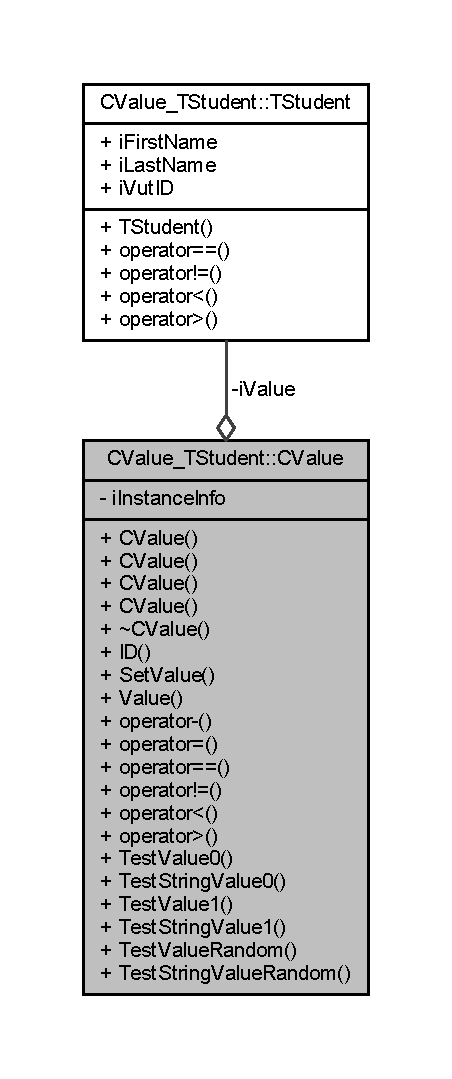
\includegraphics[width=217pt]{class_c_value___t_student_1_1_c_value__coll__graph}
\end{center}
\end{figure}
\subsection*{Public Member Functions}
\begin{DoxyCompactItemize}
\item 
\hyperlink{class_c_value___t_student_1_1_c_value_ab22934b570a1682fa933b124725230bc}{C\+Value} ()
\begin{DoxyCompactList}\small\item\em Implicit c\textquotesingle{}tor. \end{DoxyCompactList}\item 
\hyperlink{class_c_value___t_student_1_1_c_value_ae7e9f4452f6d3748cc084a95948b211c}{C\+Value} (const \hyperlink{struct_c_value___t_student_1_1_t_student}{T\+Student} a\+Value)
\begin{DoxyCompactList}\small\item\em Conversion c\textquotesingle{}tor. \end{DoxyCompactList}\item 
\hyperlink{class_c_value___t_student_1_1_c_value_a093fe369a13652f089a92884b60e0cfa}{C\+Value} (const \hyperlink{class_c_value___t_student_1_1_c_value}{C\+Value} \&a\+Value)
\begin{DoxyCompactList}\small\item\em Copy c\textquotesingle{}tor. \end{DoxyCompactList}\item 
\hyperlink{class_c_value___t_student_1_1_c_value_a488e8a348d17591900a6dabe3525b797}{C\+Value} (const char $\ast$a\+Str)
\begin{DoxyCompactList}\small\item\em String conversion c\textquotesingle{}tor. \end{DoxyCompactList}\item 
virtual \hyperlink{class_c_value___t_student_1_1_c_value_a2a4f5cdb7acace3f45674d4170ca4193}{$\sim$\+C\+Value} ()
\begin{DoxyCompactList}\small\item\em Virtual d\textquotesingle{}tor. \end{DoxyCompactList}\item 
size\+\_\+t \hyperlink{class_c_value___t_student_1_1_c_value_a1566b665478e871559c8258c95903756}{ID} () const
\begin{DoxyCompactList}\small\item\em ID getter. \end{DoxyCompactList}\item 
void \hyperlink{class_c_value___t_student_1_1_c_value_a1fcbd9b398c97c4365de889a533c90e1}{Set\+Value} (const \hyperlink{struct_c_value___t_student_1_1_t_student}{T\+Student} a\+Value)
\begin{DoxyCompactList}\small\item\em Value setter. \end{DoxyCompactList}\item 
\hyperlink{struct_c_value___t_student_1_1_t_student}{T\+Student} \hyperlink{class_c_value___t_student_1_1_c_value_a8b3771c6800a24fd9933dd1aaf30261a}{Value} () const
\begin{DoxyCompactList}\small\item\em Value getter. \end{DoxyCompactList}\item 
\hyperlink{class_c_value___t_student_1_1_c_value}{C\+Value} \hyperlink{class_c_value___t_student_1_1_c_value_a7659b2e85b6f304c7a83e2ef4f4c3f8d}{operator-\/} () const
\begin{DoxyCompactList}\small\item\em Complement operator. \end{DoxyCompactList}\item 
\hyperlink{class_c_value___t_student_1_1_c_value}{C\+Value} \& \hyperlink{class_c_value___t_student_1_1_c_value_a837c1a449684ebdb0235449f214deb9d}{operator=} (const \hyperlink{class_c_value___t_student_1_1_c_value}{C\+Value} \&a\+Value)
\begin{DoxyCompactList}\small\item\em Assigment operator. \end{DoxyCompactList}\item 
bool \hyperlink{class_c_value___t_student_1_1_c_value_a81e74014d65406bce259c0b37df25992}{operator==} (const \hyperlink{class_c_value___t_student_1_1_c_value}{C\+Value} \&a\+Value) const
\begin{DoxyCompactList}\small\item\em Comparing by Value operator. \end{DoxyCompactList}\item 
bool \hyperlink{class_c_value___t_student_1_1_c_value_a8c4c7ec16e82c22d526efe356a043361}{operator!=} (const \hyperlink{class_c_value___t_student_1_1_c_value}{C\+Value} \&a\+Value) const
\begin{DoxyCompactList}\small\item\em Comparing by Value operator. \end{DoxyCompactList}\item 
bool \hyperlink{class_c_value___t_student_1_1_c_value_a616db0b5d1db68fef3d0cdfb382e37c4}{operator$<$} (const \hyperlink{class_c_value___t_student_1_1_c_value}{C\+Value} \&a\+Value) const
\begin{DoxyCompactList}\small\item\em Comparing by Value operator. \end{DoxyCompactList}\item 
bool \hyperlink{class_c_value___t_student_1_1_c_value_a5388821b6aef1ce4a0e5411145af9d72}{operator$>$} (const \hyperlink{class_c_value___t_student_1_1_c_value}{C\+Value} \&a\+Value) const
\begin{DoxyCompactList}\small\item\em Comparing by Value operator. \end{DoxyCompactList}\end{DoxyCompactItemize}
\subsection*{Static Public Member Functions}
\begin{DoxyCompactItemize}
\item 
static \hyperlink{struct_c_value___t_student_1_1_t_student}{T\+Student} \hyperlink{class_c_value___t_student_1_1_c_value_a7e1c9e64ef5c8428df0fd56772d1240e}{Test\+Value0} ()
\begin{DoxyCompactList}\small\item\em First test value. \end{DoxyCompactList}\item 
static const char $\ast$ \hyperlink{class_c_value___t_student_1_1_c_value_a7a3fba914631fd789942450660718a32}{Test\+String\+Value0} ()
\begin{DoxyCompactList}\small\item\em First test string value. \end{DoxyCompactList}\item 
static \hyperlink{struct_c_value___t_student_1_1_t_student}{T\+Student} \hyperlink{class_c_value___t_student_1_1_c_value_a41c8aac60fd9651de611ce2220d3f352}{Test\+Value1} ()
\begin{DoxyCompactList}\small\item\em Second test value. \end{DoxyCompactList}\item 
static const char $\ast$ \hyperlink{class_c_value___t_student_1_1_c_value_a0454785a06a1974c4b969d7684b46f2b}{Test\+String\+Value1} ()
\begin{DoxyCompactList}\small\item\em Second test string value. \end{DoxyCompactList}\item 
static \hyperlink{struct_c_value___t_student_1_1_t_student}{T\+Student} \hyperlink{class_c_value___t_student_1_1_c_value_a86cd62d595805bfaaa99c7519fddff21}{Test\+Value\+Random} ()
\begin{DoxyCompactList}\small\item\em Random test value. \end{DoxyCompactList}\item 
static const char $\ast$ \hyperlink{class_c_value___t_student_1_1_c_value_af49bae0a3cb30d58c8528e168693558b}{Test\+String\+Value\+Random} ()
\begin{DoxyCompactList}\small\item\em Random test string value. \end{DoxyCompactList}\end{DoxyCompactItemize}
\subsection*{Private Attributes}
\begin{DoxyCompactItemize}
\item 
Class\+Info$<$ \hyperlink{class_c_value___t_student_1_1_c_value}{C\+Value} $>$ \hyperlink{class_c_value___t_student_1_1_c_value_aa89255973fbe024aeb90238604b599f9}{i\+Instance\+Info}
\begin{DoxyCompactList}\small\item\em Instance of the class info for usage statistics. \end{DoxyCompactList}\item 
\hyperlink{struct_c_value___t_student_1_1_t_student}{T\+Student} \hyperlink{class_c_value___t_student_1_1_c_value_a78375ada0a22e550fa030192f1786010}{i\+Value}
\begin{DoxyCompactList}\small\item\em Encapsulated {\ttfamily struct} \hyperlink{struct_c_value___t_student_1_1_t_student}{T\+Student} value. \end{DoxyCompactList}\end{DoxyCompactItemize}
\subsection*{Friends}
\begin{DoxyCompactItemize}
\item 
std\+::ostream \& \hyperlink{class_c_value___t_student_1_1_c_value_a3d28097fae6bdd5a8146d9ab90f8b62f}{operator$<$$<$} (std\+::ostream \&a\+O\+Stream, const \hyperlink{class_c_value___t_student_1_1_c_value}{C\+Value} \&a\+Value)
\begin{DoxyCompactList}\small\item\em Output to the stream operator. ({\itshape serialization}) \end{DoxyCompactList}\item 
std\+::istream \& \hyperlink{class_c_value___t_student_1_1_c_value_aba05045ca890e398c1211784aebbc9ed}{operator$>$$>$} (std\+::istream \&a\+I\+Stream, \hyperlink{class_c_value___t_student_1_1_c_value}{C\+Value} \&a\+Value)
\begin{DoxyCompactList}\small\item\em Input from the stream operator. ({\itshape deserialization}) \end{DoxyCompactList}\end{DoxyCompactItemize}


\subsection{Detailed Description}
\hyperlink{class_c_value___t_student_1_1_c_value}{C\+Value} class ({\ttfamily \hyperlink{struct_c_value___t_student_1_1_t_student}{T\+Student}} variant) 

Definition of \hyperlink{class_c_value___t_student_1_1_c_value}{C\+Value} class ({\ttfamily \hyperlink{struct_c_value___t_student_1_1_t_student}{T\+Student}} variant). There is defined all common methods and attributes. 

Definition at line 73 of file C\+Value\+\_\+\+T\+Student.\+h.



\subsection{Constructor \& Destructor Documentation}
\mbox{\Hypertarget{class_c_value___t_student_1_1_c_value_ab22934b570a1682fa933b124725230bc}\label{class_c_value___t_student_1_1_c_value_ab22934b570a1682fa933b124725230bc}} 
\index{C\+Value\+\_\+\+T\+Student\+::\+C\+Value@{C\+Value\+\_\+\+T\+Student\+::\+C\+Value}!C\+Value@{C\+Value}}
\index{C\+Value@{C\+Value}!C\+Value\+\_\+\+T\+Student\+::\+C\+Value@{C\+Value\+\_\+\+T\+Student\+::\+C\+Value}}
\subsubsection{\texorpdfstring{C\+Value()}{CValue()}\hspace{0.1cm}{\footnotesize\ttfamily [1/4]}}
{\footnotesize\ttfamily C\+Value\+\_\+\+T\+Student\+::\+C\+Value\+::\+C\+Value (\begin{DoxyParamCaption}{ }\end{DoxyParamCaption})\hspace{0.3cm}{\ttfamily [inline]}}



Implicit c\textquotesingle{}tor. 



Definition at line 82 of file C\+Value\+\_\+\+T\+Student.\+h.

\mbox{\Hypertarget{class_c_value___t_student_1_1_c_value_ae7e9f4452f6d3748cc084a95948b211c}\label{class_c_value___t_student_1_1_c_value_ae7e9f4452f6d3748cc084a95948b211c}} 
\index{C\+Value\+\_\+\+T\+Student\+::\+C\+Value@{C\+Value\+\_\+\+T\+Student\+::\+C\+Value}!C\+Value@{C\+Value}}
\index{C\+Value@{C\+Value}!C\+Value\+\_\+\+T\+Student\+::\+C\+Value@{C\+Value\+\_\+\+T\+Student\+::\+C\+Value}}
\subsubsection{\texorpdfstring{C\+Value()}{CValue()}\hspace{0.1cm}{\footnotesize\ttfamily [2/4]}}
{\footnotesize\ttfamily C\+Value\+\_\+\+T\+Student\+::\+C\+Value\+::\+C\+Value (\begin{DoxyParamCaption}\item[{const \hyperlink{struct_c_value___t_student_1_1_t_student}{T\+Student}}]{a\+Value }\end{DoxyParamCaption})\hspace{0.3cm}{\ttfamily [inline]}, {\ttfamily [explicit]}}



Conversion c\textquotesingle{}tor. 

Pointer attributes are initialised to the {\ttfamily this} value. 
\begin{DoxyParams}[1]{Parameters}
\mbox{\tt in}  & {\em a\+Value} & New \hyperlink{struct_c_value___t_student_1_1_t_student}{T\+Student} value \\
\hline
\end{DoxyParams}


Definition at line 89 of file C\+Value\+\_\+\+T\+Student.\+h.

\mbox{\Hypertarget{class_c_value___t_student_1_1_c_value_a093fe369a13652f089a92884b60e0cfa}\label{class_c_value___t_student_1_1_c_value_a093fe369a13652f089a92884b60e0cfa}} 
\index{C\+Value\+\_\+\+T\+Student\+::\+C\+Value@{C\+Value\+\_\+\+T\+Student\+::\+C\+Value}!C\+Value@{C\+Value}}
\index{C\+Value@{C\+Value}!C\+Value\+\_\+\+T\+Student\+::\+C\+Value@{C\+Value\+\_\+\+T\+Student\+::\+C\+Value}}
\subsubsection{\texorpdfstring{C\+Value()}{CValue()}\hspace{0.1cm}{\footnotesize\ttfamily [3/4]}}
{\footnotesize\ttfamily C\+Value\+\_\+\+T\+Student\+::\+C\+Value\+::\+C\+Value (\begin{DoxyParamCaption}\item[{const \hyperlink{class_c_value___t_student_1_1_c_value}{C\+Value} \&}]{a\+Value }\end{DoxyParamCaption})\hspace{0.3cm}{\ttfamily [inline]}}



Copy c\textquotesingle{}tor. 

Create new instance by copying only {\ttfamily i\+Value} parameter. 
\begin{DoxyParams}[1]{Parameters}
\mbox{\tt in}  & {\em a\+Value} & Original instance for copying \\
\hline
\end{DoxyParams}


Definition at line 96 of file C\+Value\+\_\+\+T\+Student.\+h.

\mbox{\Hypertarget{class_c_value___t_student_1_1_c_value_a488e8a348d17591900a6dabe3525b797}\label{class_c_value___t_student_1_1_c_value_a488e8a348d17591900a6dabe3525b797}} 
\index{C\+Value\+\_\+\+T\+Student\+::\+C\+Value@{C\+Value\+\_\+\+T\+Student\+::\+C\+Value}!C\+Value@{C\+Value}}
\index{C\+Value@{C\+Value}!C\+Value\+\_\+\+T\+Student\+::\+C\+Value@{C\+Value\+\_\+\+T\+Student\+::\+C\+Value}}
\subsubsection{\texorpdfstring{C\+Value()}{CValue()}\hspace{0.1cm}{\footnotesize\ttfamily [4/4]}}
{\footnotesize\ttfamily C\+Value\+\_\+\+T\+Student\+::\+C\+Value\+::\+C\+Value (\begin{DoxyParamCaption}\item[{const char $\ast$}]{a\+Str }\end{DoxyParamCaption})\hspace{0.3cm}{\ttfamily [inline]}, {\ttfamily [explicit]}}



String conversion c\textquotesingle{}tor. 

Create new instance from Value in the string. Pointer attributes are initialised to the {\ttfamily this} value. 
\begin{DoxyParams}[1]{Parameters}
\mbox{\tt in}  & {\em a\+Str} & Plain C string with string value convertable to the \hyperlink{struct_c_value___t_student_1_1_t_student}{T\+Student} Vut\+ID value. \\
\hline
\end{DoxyParams}


Definition at line 103 of file C\+Value\+\_\+\+T\+Student.\+h.

\mbox{\Hypertarget{class_c_value___t_student_1_1_c_value_a2a4f5cdb7acace3f45674d4170ca4193}\label{class_c_value___t_student_1_1_c_value_a2a4f5cdb7acace3f45674d4170ca4193}} 
\index{C\+Value\+\_\+\+T\+Student\+::\+C\+Value@{C\+Value\+\_\+\+T\+Student\+::\+C\+Value}!````~C\+Value@{$\sim$\+C\+Value}}
\index{````~C\+Value@{$\sim$\+C\+Value}!C\+Value\+\_\+\+T\+Student\+::\+C\+Value@{C\+Value\+\_\+\+T\+Student\+::\+C\+Value}}
\subsubsection{\texorpdfstring{$\sim$\+C\+Value()}{~CValue()}}
{\footnotesize\ttfamily virtual C\+Value\+\_\+\+T\+Student\+::\+C\+Value\+::$\sim$\+C\+Value (\begin{DoxyParamCaption}{ }\end{DoxyParamCaption})\hspace{0.3cm}{\ttfamily [inline]}, {\ttfamily [virtual]}}



Virtual d\textquotesingle{}tor. 



Definition at line 112 of file C\+Value\+\_\+\+T\+Student.\+h.



\subsection{Member Function Documentation}
\mbox{\Hypertarget{class_c_value___t_student_1_1_c_value_a1566b665478e871559c8258c95903756}\label{class_c_value___t_student_1_1_c_value_a1566b665478e871559c8258c95903756}} 
\index{C\+Value\+\_\+\+T\+Student\+::\+C\+Value@{C\+Value\+\_\+\+T\+Student\+::\+C\+Value}!ID@{ID}}
\index{ID@{ID}!C\+Value\+\_\+\+T\+Student\+::\+C\+Value@{C\+Value\+\_\+\+T\+Student\+::\+C\+Value}}
\subsubsection{\texorpdfstring{I\+D()}{ID()}}
{\footnotesize\ttfamily size\+\_\+t C\+Value\+\_\+\+T\+Student\+::\+C\+Value\+::\+ID (\begin{DoxyParamCaption}{ }\end{DoxyParamCaption}) const\hspace{0.3cm}{\ttfamily [inline]}}



ID getter. 

\begin{DoxyReturn}{Returns}
Unique instance ID 
\end{DoxyReturn}


Definition at line 121 of file C\+Value\+\_\+\+T\+Student.\+h.

\mbox{\Hypertarget{class_c_value___t_student_1_1_c_value_a8c4c7ec16e82c22d526efe356a043361}\label{class_c_value___t_student_1_1_c_value_a8c4c7ec16e82c22d526efe356a043361}} 
\index{C\+Value\+\_\+\+T\+Student\+::\+C\+Value@{C\+Value\+\_\+\+T\+Student\+::\+C\+Value}!operator"!=@{operator"!=}}
\index{operator"!=@{operator"!=}!C\+Value\+\_\+\+T\+Student\+::\+C\+Value@{C\+Value\+\_\+\+T\+Student\+::\+C\+Value}}
\subsubsection{\texorpdfstring{operator"!=()}{operator!=()}}
{\footnotesize\ttfamily bool C\+Value\+\_\+\+T\+Student\+::\+C\+Value\+::operator!= (\begin{DoxyParamCaption}\item[{const \hyperlink{class_c_value___t_student_1_1_c_value}{C\+Value} \&}]{a\+Value }\end{DoxyParamCaption}) const\hspace{0.3cm}{\ttfamily [inline]}}



Comparing by Value operator. 

\begin{DoxyReturn}{Returns}
Return {\ttfamily bool} result of comparation 
\end{DoxyReturn}


Definition at line 174 of file C\+Value\+\_\+\+T\+Student.\+h.

\mbox{\Hypertarget{class_c_value___t_student_1_1_c_value_a7659b2e85b6f304c7a83e2ef4f4c3f8d}\label{class_c_value___t_student_1_1_c_value_a7659b2e85b6f304c7a83e2ef4f4c3f8d}} 
\index{C\+Value\+\_\+\+T\+Student\+::\+C\+Value@{C\+Value\+\_\+\+T\+Student\+::\+C\+Value}!operator-\/@{operator-\/}}
\index{operator-\/@{operator-\/}!C\+Value\+\_\+\+T\+Student\+::\+C\+Value@{C\+Value\+\_\+\+T\+Student\+::\+C\+Value}}
\subsubsection{\texorpdfstring{operator-\/()}{operator-()}}
{\footnotesize\ttfamily \hyperlink{class_c_value___t_student_1_1_c_value}{C\+Value} C\+Value\+\_\+\+T\+Student\+::\+C\+Value\+::operator-\/ (\begin{DoxyParamCaption}{ }\end{DoxyParamCaption}) const\hspace{0.3cm}{\ttfamily [inline]}}



Complement operator. 

\begin{DoxyReturn}{Returns}
\hyperlink{class_c_value___t_student_1_1_c_value}{C\+Value} instance with complemented attribute Value. 
\end{DoxyReturn}


Definition at line 147 of file C\+Value\+\_\+\+T\+Student.\+h.

\mbox{\Hypertarget{class_c_value___t_student_1_1_c_value_a616db0b5d1db68fef3d0cdfb382e37c4}\label{class_c_value___t_student_1_1_c_value_a616db0b5d1db68fef3d0cdfb382e37c4}} 
\index{C\+Value\+\_\+\+T\+Student\+::\+C\+Value@{C\+Value\+\_\+\+T\+Student\+::\+C\+Value}!operator$<$@{operator$<$}}
\index{operator$<$@{operator$<$}!C\+Value\+\_\+\+T\+Student\+::\+C\+Value@{C\+Value\+\_\+\+T\+Student\+::\+C\+Value}}
\subsubsection{\texorpdfstring{operator$<$()}{operator<()}}
{\footnotesize\ttfamily bool C\+Value\+\_\+\+T\+Student\+::\+C\+Value\+::operator$<$ (\begin{DoxyParamCaption}\item[{const \hyperlink{class_c_value___t_student_1_1_c_value}{C\+Value} \&}]{a\+Value }\end{DoxyParamCaption}) const\hspace{0.3cm}{\ttfamily [inline]}}



Comparing by Value operator. 

\begin{DoxyReturn}{Returns}
Return {\ttfamily bool} result of comparation 
\end{DoxyReturn}


Definition at line 182 of file C\+Value\+\_\+\+T\+Student.\+h.

\mbox{\Hypertarget{class_c_value___t_student_1_1_c_value_a837c1a449684ebdb0235449f214deb9d}\label{class_c_value___t_student_1_1_c_value_a837c1a449684ebdb0235449f214deb9d}} 
\index{C\+Value\+\_\+\+T\+Student\+::\+C\+Value@{C\+Value\+\_\+\+T\+Student\+::\+C\+Value}!operator=@{operator=}}
\index{operator=@{operator=}!C\+Value\+\_\+\+T\+Student\+::\+C\+Value@{C\+Value\+\_\+\+T\+Student\+::\+C\+Value}}
\subsubsection{\texorpdfstring{operator=()}{operator=()}}
{\footnotesize\ttfamily \hyperlink{class_c_value___t_student_1_1_c_value}{C\+Value}\& C\+Value\+\_\+\+T\+Student\+::\+C\+Value\+::operator= (\begin{DoxyParamCaption}\item[{const \hyperlink{class_c_value___t_student_1_1_c_value}{C\+Value} \&}]{a\+Value }\end{DoxyParamCaption})\hspace{0.3cm}{\ttfamily [inline]}}



Assigment operator. 

\begin{DoxyReturn}{Returns}
\hyperlink{class_c_value___t_student_1_1_c_value}{C\+Value} instance with copied attribute Value. 
\end{DoxyReturn}


Definition at line 157 of file C\+Value\+\_\+\+T\+Student.\+h.

\mbox{\Hypertarget{class_c_value___t_student_1_1_c_value_a81e74014d65406bce259c0b37df25992}\label{class_c_value___t_student_1_1_c_value_a81e74014d65406bce259c0b37df25992}} 
\index{C\+Value\+\_\+\+T\+Student\+::\+C\+Value@{C\+Value\+\_\+\+T\+Student\+::\+C\+Value}!operator==@{operator==}}
\index{operator==@{operator==}!C\+Value\+\_\+\+T\+Student\+::\+C\+Value@{C\+Value\+\_\+\+T\+Student\+::\+C\+Value}}
\subsubsection{\texorpdfstring{operator==()}{operator==()}}
{\footnotesize\ttfamily bool C\+Value\+\_\+\+T\+Student\+::\+C\+Value\+::operator== (\begin{DoxyParamCaption}\item[{const \hyperlink{class_c_value___t_student_1_1_c_value}{C\+Value} \&}]{a\+Value }\end{DoxyParamCaption}) const\hspace{0.3cm}{\ttfamily [inline]}}



Comparing by Value operator. 

\begin{DoxyReturn}{Returns}
Return {\ttfamily bool} result of comparation 
\end{DoxyReturn}


Definition at line 166 of file C\+Value\+\_\+\+T\+Student.\+h.

\mbox{\Hypertarget{class_c_value___t_student_1_1_c_value_a5388821b6aef1ce4a0e5411145af9d72}\label{class_c_value___t_student_1_1_c_value_a5388821b6aef1ce4a0e5411145af9d72}} 
\index{C\+Value\+\_\+\+T\+Student\+::\+C\+Value@{C\+Value\+\_\+\+T\+Student\+::\+C\+Value}!operator$>$@{operator$>$}}
\index{operator$>$@{operator$>$}!C\+Value\+\_\+\+T\+Student\+::\+C\+Value@{C\+Value\+\_\+\+T\+Student\+::\+C\+Value}}
\subsubsection{\texorpdfstring{operator$>$()}{operator>()}}
{\footnotesize\ttfamily bool C\+Value\+\_\+\+T\+Student\+::\+C\+Value\+::operator$>$ (\begin{DoxyParamCaption}\item[{const \hyperlink{class_c_value___t_student_1_1_c_value}{C\+Value} \&}]{a\+Value }\end{DoxyParamCaption}) const\hspace{0.3cm}{\ttfamily [inline]}}



Comparing by Value operator. 

\begin{DoxyReturn}{Returns}
Return {\ttfamily bool} result of comparation 
\end{DoxyReturn}


Definition at line 190 of file C\+Value\+\_\+\+T\+Student.\+h.

\mbox{\Hypertarget{class_c_value___t_student_1_1_c_value_a1fcbd9b398c97c4365de889a533c90e1}\label{class_c_value___t_student_1_1_c_value_a1fcbd9b398c97c4365de889a533c90e1}} 
\index{C\+Value\+\_\+\+T\+Student\+::\+C\+Value@{C\+Value\+\_\+\+T\+Student\+::\+C\+Value}!Set\+Value@{Set\+Value}}
\index{Set\+Value@{Set\+Value}!C\+Value\+\_\+\+T\+Student\+::\+C\+Value@{C\+Value\+\_\+\+T\+Student\+::\+C\+Value}}
\subsubsection{\texorpdfstring{Set\+Value()}{SetValue()}}
{\footnotesize\ttfamily void C\+Value\+\_\+\+T\+Student\+::\+C\+Value\+::\+Set\+Value (\begin{DoxyParamCaption}\item[{const \hyperlink{struct_c_value___t_student_1_1_t_student}{T\+Student}}]{a\+Value }\end{DoxyParamCaption})\hspace{0.3cm}{\ttfamily [inline]}}



Value setter. 


\begin{DoxyParams}[1]{Parameters}
\mbox{\tt in}  & {\em a\+Value} & New Value \\
\hline
\end{DoxyParams}


Definition at line 130 of file C\+Value\+\_\+\+T\+Student.\+h.

\mbox{\Hypertarget{class_c_value___t_student_1_1_c_value_a7a3fba914631fd789942450660718a32}\label{class_c_value___t_student_1_1_c_value_a7a3fba914631fd789942450660718a32}} 
\index{C\+Value\+\_\+\+T\+Student\+::\+C\+Value@{C\+Value\+\_\+\+T\+Student\+::\+C\+Value}!Test\+String\+Value0@{Test\+String\+Value0}}
\index{Test\+String\+Value0@{Test\+String\+Value0}!C\+Value\+\_\+\+T\+Student\+::\+C\+Value@{C\+Value\+\_\+\+T\+Student\+::\+C\+Value}}
\subsubsection{\texorpdfstring{Test\+String\+Value0()}{TestStringValue0()}}
{\footnotesize\ttfamily static const char$\ast$ C\+Value\+\_\+\+T\+Student\+::\+C\+Value\+::\+Test\+String\+Value0 (\begin{DoxyParamCaption}{ }\end{DoxyParamCaption})\hspace{0.3cm}{\ttfamily [inline]}, {\ttfamily [static]}}



First test string value. 

\begin{DoxyReturn}{Returns}
Return string -\/ \char`\"{}0\char`\"{} 
\end{DoxyReturn}
\begin{DoxyNote}{Note}
Useful for automated testing of \hyperlink{class_c_value___t_student_1_1_c_value}{C\+Value} functionality 
\end{DoxyNote}


Definition at line 233 of file C\+Value\+\_\+\+T\+Student.\+h.

\mbox{\Hypertarget{class_c_value___t_student_1_1_c_value_a0454785a06a1974c4b969d7684b46f2b}\label{class_c_value___t_student_1_1_c_value_a0454785a06a1974c4b969d7684b46f2b}} 
\index{C\+Value\+\_\+\+T\+Student\+::\+C\+Value@{C\+Value\+\_\+\+T\+Student\+::\+C\+Value}!Test\+String\+Value1@{Test\+String\+Value1}}
\index{Test\+String\+Value1@{Test\+String\+Value1}!C\+Value\+\_\+\+T\+Student\+::\+C\+Value@{C\+Value\+\_\+\+T\+Student\+::\+C\+Value}}
\subsubsection{\texorpdfstring{Test\+String\+Value1()}{TestStringValue1()}}
{\footnotesize\ttfamily static const char$\ast$ C\+Value\+\_\+\+T\+Student\+::\+C\+Value\+::\+Test\+String\+Value1 (\begin{DoxyParamCaption}{ }\end{DoxyParamCaption})\hspace{0.3cm}{\ttfamily [inline]}, {\ttfamily [static]}}



Second test string value. 

\begin{DoxyReturn}{Returns}
Return string -\/ \char`\"{}1\char`\"{} 
\end{DoxyReturn}
\begin{DoxyNote}{Note}
Useful for automated testing of \hyperlink{class_c_value___t_student_1_1_c_value}{C\+Value} functionality 
\end{DoxyNote}


Definition at line 251 of file C\+Value\+\_\+\+T\+Student.\+h.

\mbox{\Hypertarget{class_c_value___t_student_1_1_c_value_af49bae0a3cb30d58c8528e168693558b}\label{class_c_value___t_student_1_1_c_value_af49bae0a3cb30d58c8528e168693558b}} 
\index{C\+Value\+\_\+\+T\+Student\+::\+C\+Value@{C\+Value\+\_\+\+T\+Student\+::\+C\+Value}!Test\+String\+Value\+Random@{Test\+String\+Value\+Random}}
\index{Test\+String\+Value\+Random@{Test\+String\+Value\+Random}!C\+Value\+\_\+\+T\+Student\+::\+C\+Value@{C\+Value\+\_\+\+T\+Student\+::\+C\+Value}}
\subsubsection{\texorpdfstring{Test\+String\+Value\+Random()}{TestStringValueRandom()}}
{\footnotesize\ttfamily static const char$\ast$ C\+Value\+\_\+\+T\+Student\+::\+C\+Value\+::\+Test\+String\+Value\+Random (\begin{DoxyParamCaption}{ }\end{DoxyParamCaption})\hspace{0.3cm}{\ttfamily [inline]}, {\ttfamily [static]}}



Random test string value. 

\begin{DoxyReturn}{Returns}
Return string with random \hyperlink{struct_c_value___t_student_1_1_t_student}{T\+Student} value 
\end{DoxyReturn}
\begin{DoxyNote}{Note}
Useful for automated testing of \hyperlink{class_c_value___t_student_1_1_c_value}{C\+Value} functionality 
\end{DoxyNote}


Definition at line 269 of file C\+Value\+\_\+\+T\+Student.\+h.

\mbox{\Hypertarget{class_c_value___t_student_1_1_c_value_a7e1c9e64ef5c8428df0fd56772d1240e}\label{class_c_value___t_student_1_1_c_value_a7e1c9e64ef5c8428df0fd56772d1240e}} 
\index{C\+Value\+\_\+\+T\+Student\+::\+C\+Value@{C\+Value\+\_\+\+T\+Student\+::\+C\+Value}!Test\+Value0@{Test\+Value0}}
\index{Test\+Value0@{Test\+Value0}!C\+Value\+\_\+\+T\+Student\+::\+C\+Value@{C\+Value\+\_\+\+T\+Student\+::\+C\+Value}}
\subsubsection{\texorpdfstring{Test\+Value0()}{TestValue0()}}
{\footnotesize\ttfamily static \hyperlink{struct_c_value___t_student_1_1_t_student}{T\+Student} C\+Value\+\_\+\+T\+Student\+::\+C\+Value\+::\+Test\+Value0 (\begin{DoxyParamCaption}{ }\end{DoxyParamCaption})\hspace{0.3cm}{\ttfamily [inline]}, {\ttfamily [static]}}



First test value. 

\begin{DoxyReturn}{Returns}
Return T\+Week\+Day value (Student0) 
\end{DoxyReturn}
\begin{DoxyNote}{Note}
Useful for automated testing of \hyperlink{class_c_value___t_student_1_1_c_value}{C\+Value} functionality 
\end{DoxyNote}


Definition at line 224 of file C\+Value\+\_\+\+T\+Student.\+h.

\mbox{\Hypertarget{class_c_value___t_student_1_1_c_value_a41c8aac60fd9651de611ce2220d3f352}\label{class_c_value___t_student_1_1_c_value_a41c8aac60fd9651de611ce2220d3f352}} 
\index{C\+Value\+\_\+\+T\+Student\+::\+C\+Value@{C\+Value\+\_\+\+T\+Student\+::\+C\+Value}!Test\+Value1@{Test\+Value1}}
\index{Test\+Value1@{Test\+Value1}!C\+Value\+\_\+\+T\+Student\+::\+C\+Value@{C\+Value\+\_\+\+T\+Student\+::\+C\+Value}}
\subsubsection{\texorpdfstring{Test\+Value1()}{TestValue1()}}
{\footnotesize\ttfamily static \hyperlink{struct_c_value___t_student_1_1_t_student}{T\+Student} C\+Value\+\_\+\+T\+Student\+::\+C\+Value\+::\+Test\+Value1 (\begin{DoxyParamCaption}{ }\end{DoxyParamCaption})\hspace{0.3cm}{\ttfamily [inline]}, {\ttfamily [static]}}



Second test value. 

\begin{DoxyReturn}{Returns}
Return \hyperlink{struct_c_value___t_student_1_1_t_student}{T\+Student} value (Student1) 
\end{DoxyReturn}
\begin{DoxyNote}{Note}
Useful for automated testing of \hyperlink{class_c_value___t_student_1_1_c_value}{C\+Value} functionality 
\end{DoxyNote}


Definition at line 242 of file C\+Value\+\_\+\+T\+Student.\+h.

\mbox{\Hypertarget{class_c_value___t_student_1_1_c_value_a86cd62d595805bfaaa99c7519fddff21}\label{class_c_value___t_student_1_1_c_value_a86cd62d595805bfaaa99c7519fddff21}} 
\index{C\+Value\+\_\+\+T\+Student\+::\+C\+Value@{C\+Value\+\_\+\+T\+Student\+::\+C\+Value}!Test\+Value\+Random@{Test\+Value\+Random}}
\index{Test\+Value\+Random@{Test\+Value\+Random}!C\+Value\+\_\+\+T\+Student\+::\+C\+Value@{C\+Value\+\_\+\+T\+Student\+::\+C\+Value}}
\subsubsection{\texorpdfstring{Test\+Value\+Random()}{TestValueRandom()}}
{\footnotesize\ttfamily static \hyperlink{struct_c_value___t_student_1_1_t_student}{T\+Student} C\+Value\+\_\+\+T\+Student\+::\+C\+Value\+::\+Test\+Value\+Random (\begin{DoxyParamCaption}{ }\end{DoxyParamCaption})\hspace{0.3cm}{\ttfamily [inline]}, {\ttfamily [static]}}



Random test value. 

\begin{DoxyReturn}{Returns}
Return random \hyperlink{struct_c_value___t_student_1_1_t_student}{T\+Student} value 
\end{DoxyReturn}
\begin{DoxyNote}{Note}
Useful for automated testing of \hyperlink{class_c_value___t_student_1_1_c_value}{C\+Value} functionality 
\end{DoxyNote}


Definition at line 260 of file C\+Value\+\_\+\+T\+Student.\+h.

\mbox{\Hypertarget{class_c_value___t_student_1_1_c_value_a8b3771c6800a24fd9933dd1aaf30261a}\label{class_c_value___t_student_1_1_c_value_a8b3771c6800a24fd9933dd1aaf30261a}} 
\index{C\+Value\+\_\+\+T\+Student\+::\+C\+Value@{C\+Value\+\_\+\+T\+Student\+::\+C\+Value}!Value@{Value}}
\index{Value@{Value}!C\+Value\+\_\+\+T\+Student\+::\+C\+Value@{C\+Value\+\_\+\+T\+Student\+::\+C\+Value}}
\subsubsection{\texorpdfstring{Value()}{Value()}}
{\footnotesize\ttfamily \hyperlink{struct_c_value___t_student_1_1_t_student}{T\+Student} C\+Value\+\_\+\+T\+Student\+::\+C\+Value\+::\+Value (\begin{DoxyParamCaption}{ }\end{DoxyParamCaption}) const\hspace{0.3cm}{\ttfamily [inline]}}



Value getter. 

\begin{DoxyReturn}{Returns}
Actual {\ttfamily bool} {\ttfamily Value} 
\end{DoxyReturn}


Definition at line 138 of file C\+Value\+\_\+\+T\+Student.\+h.



\subsection{Friends And Related Function Documentation}
\mbox{\Hypertarget{class_c_value___t_student_1_1_c_value_a3d28097fae6bdd5a8146d9ab90f8b62f}\label{class_c_value___t_student_1_1_c_value_a3d28097fae6bdd5a8146d9ab90f8b62f}} 
\index{C\+Value\+\_\+\+T\+Student\+::\+C\+Value@{C\+Value\+\_\+\+T\+Student\+::\+C\+Value}!operator$<$$<$@{operator$<$$<$}}
\index{operator$<$$<$@{operator$<$$<$}!C\+Value\+\_\+\+T\+Student\+::\+C\+Value@{C\+Value\+\_\+\+T\+Student\+::\+C\+Value}}
\subsubsection{\texorpdfstring{operator$<$$<$}{operator<<}}
{\footnotesize\ttfamily std\+::ostream\& operator$<$$<$ (\begin{DoxyParamCaption}\item[{std\+::ostream \&}]{a\+O\+Stream,  }\item[{const \hyperlink{class_c_value___t_student_1_1_c_value}{C\+Value} \&}]{a\+Value }\end{DoxyParamCaption})\hspace{0.3cm}{\ttfamily [friend]}}



Output to the stream operator. ({\itshape serialization}) 


\begin{DoxyParams}[1]{Parameters}
\mbox{\tt in}  & {\em a\+O\+Stream} & Output stream \\
\hline
\mbox{\tt in}  & {\em a\+Value} & Serialized instantion of \hyperlink{class_c_value___t_student_1_1_c_value}{C\+Value} \\
\hline
\end{DoxyParams}
\begin{DoxyReturn}{Returns}
Return {\ttfamily std\+::ostream} with serialized Value 
\end{DoxyReturn}


Definition at line 200 of file C\+Value\+\_\+\+T\+Student.\+h.

\mbox{\Hypertarget{class_c_value___t_student_1_1_c_value_aba05045ca890e398c1211784aebbc9ed}\label{class_c_value___t_student_1_1_c_value_aba05045ca890e398c1211784aebbc9ed}} 
\index{C\+Value\+\_\+\+T\+Student\+::\+C\+Value@{C\+Value\+\_\+\+T\+Student\+::\+C\+Value}!operator$>$$>$@{operator$>$$>$}}
\index{operator$>$$>$@{operator$>$$>$}!C\+Value\+\_\+\+T\+Student\+::\+C\+Value@{C\+Value\+\_\+\+T\+Student\+::\+C\+Value}}
\subsubsection{\texorpdfstring{operator$>$$>$}{operator>>}}
{\footnotesize\ttfamily std\+::istream\& operator$>$$>$ (\begin{DoxyParamCaption}\item[{std\+::istream \&}]{a\+I\+Stream,  }\item[{\hyperlink{class_c_value___t_student_1_1_c_value}{C\+Value} \&}]{a\+Value }\end{DoxyParamCaption})\hspace{0.3cm}{\ttfamily [friend]}}



Input from the stream operator. ({\itshape deserialization}) 


\begin{DoxyParams}[1]{Parameters}
\mbox{\tt in}  & {\em a\+I\+Stream} & Input stream \\
\hline
\mbox{\tt out}  & {\em a\+Value} & Place for deserialized instantion of \hyperlink{class_c_value___t_student_1_1_c_value}{C\+Value} \\
\hline
\end{DoxyParams}
\begin{DoxyReturn}{Returns}
Return rest of {\ttfamily std\+::istream} 
\end{DoxyReturn}


Definition at line 211 of file C\+Value\+\_\+\+T\+Student.\+h.



\subsection{Member Data Documentation}
\mbox{\Hypertarget{class_c_value___t_student_1_1_c_value_aa89255973fbe024aeb90238604b599f9}\label{class_c_value___t_student_1_1_c_value_aa89255973fbe024aeb90238604b599f9}} 
\index{C\+Value\+\_\+\+T\+Student\+::\+C\+Value@{C\+Value\+\_\+\+T\+Student\+::\+C\+Value}!i\+Instance\+Info@{i\+Instance\+Info}}
\index{i\+Instance\+Info@{i\+Instance\+Info}!C\+Value\+\_\+\+T\+Student\+::\+C\+Value@{C\+Value\+\_\+\+T\+Student\+::\+C\+Value}}
\subsubsection{\texorpdfstring{i\+Instance\+Info}{iInstanceInfo}}
{\footnotesize\ttfamily Class\+Info$<$\hyperlink{class_c_value___t_student_1_1_c_value}{C\+Value}$>$ C\+Value\+\_\+\+T\+Student\+::\+C\+Value\+::i\+Instance\+Info\hspace{0.3cm}{\ttfamily [private]}}



Instance of the class info for usage statistics. 



Definition at line 75 of file C\+Value\+\_\+\+T\+Student.\+h.

\mbox{\Hypertarget{class_c_value___t_student_1_1_c_value_a78375ada0a22e550fa030192f1786010}\label{class_c_value___t_student_1_1_c_value_a78375ada0a22e550fa030192f1786010}} 
\index{C\+Value\+\_\+\+T\+Student\+::\+C\+Value@{C\+Value\+\_\+\+T\+Student\+::\+C\+Value}!i\+Value@{i\+Value}}
\index{i\+Value@{i\+Value}!C\+Value\+\_\+\+T\+Student\+::\+C\+Value@{C\+Value\+\_\+\+T\+Student\+::\+C\+Value}}
\subsubsection{\texorpdfstring{i\+Value}{iValue}}
{\footnotesize\ttfamily \hyperlink{struct_c_value___t_student_1_1_t_student}{T\+Student} C\+Value\+\_\+\+T\+Student\+::\+C\+Value\+::i\+Value\hspace{0.3cm}{\ttfamily [private]}}



Encapsulated {\ttfamily struct} \hyperlink{struct_c_value___t_student_1_1_t_student}{T\+Student} value. 



Definition at line 76 of file C\+Value\+\_\+\+T\+Student.\+h.



The documentation for this class was generated from the following file\+:\begin{DoxyCompactItemize}
\item 
\hyperlink{_c_value___t_student_8h}{C\+Value\+\_\+\+T\+Student.\+h}\end{DoxyCompactItemize}

\hypertarget{class_c_value__long_1_1_c_value}{}\section{C\+Value\+\_\+long\+:\+:C\+Value Class Reference}
\label{class_c_value__long_1_1_c_value}\index{C\+Value\+\_\+long\+::\+C\+Value@{C\+Value\+\_\+long\+::\+C\+Value}}


\hyperlink{class_c_value__long_1_1_c_value}{C\+Value} class ({\ttfamily long} variant)  




{\ttfamily \#include $<$C\+Value\+\_\+long.\+h$>$}



Collaboration diagram for C\+Value\+\_\+long\+:\+:C\+Value\+:\nopagebreak
\begin{figure}[H]
\begin{center}
\leavevmode
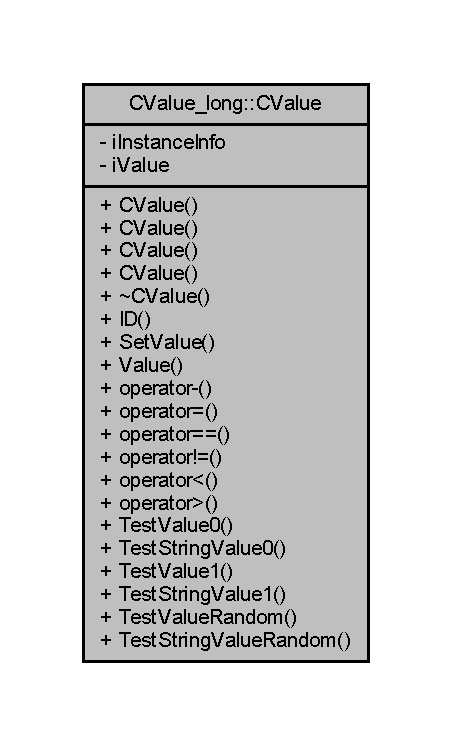
\includegraphics[width=217pt]{class_c_value__long_1_1_c_value__coll__graph}
\end{center}
\end{figure}
\subsection*{Public Member Functions}
\begin{DoxyCompactItemize}
\item 
\hyperlink{class_c_value__long_1_1_c_value_a40c175a667125b6dc8faa84b0424ce4d}{C\+Value} ()
\begin{DoxyCompactList}\small\item\em Implicit c\textquotesingle{}tor. \end{DoxyCompactList}\item 
\hyperlink{class_c_value__long_1_1_c_value_a5c36e74c9d748c86e4061b38ac1749b7}{C\+Value} (const long a\+Value)
\begin{DoxyCompactList}\small\item\em Conversion c\textquotesingle{}tor. \end{DoxyCompactList}\item 
\hyperlink{class_c_value__long_1_1_c_value_a88c1a4c4f4f157417b382f2ea9f7836d}{C\+Value} (const \hyperlink{class_c_value__long_1_1_c_value}{C\+Value} \&a\+Value)
\begin{DoxyCompactList}\small\item\em Copy c\textquotesingle{}tor. \end{DoxyCompactList}\item 
\hyperlink{class_c_value__long_1_1_c_value_a098c962b0bcf399ec9179ac5dd9cc42f}{C\+Value} (const char $\ast$a\+Str)
\begin{DoxyCompactList}\small\item\em String conversion c\textquotesingle{}tor. \end{DoxyCompactList}\item 
virtual \hyperlink{class_c_value__long_1_1_c_value_aedefeae635e586789cd62bd9ec5401de}{$\sim$\+C\+Value} () noexcept(false)
\begin{DoxyCompactList}\small\item\em Virtual d\textquotesingle{}tor. \end{DoxyCompactList}\item 
size\+\_\+t \hyperlink{class_c_value__long_1_1_c_value_aa7ef0a671a39efbc567fa9c6a1fb49a8}{ID} () const
\begin{DoxyCompactList}\small\item\em ID getter. \end{DoxyCompactList}\item 
void \hyperlink{class_c_value__long_1_1_c_value_a8caf06185aa1c4ecd60d70c5d0d02631}{Set\+Value} (const long a\+Value)
\begin{DoxyCompactList}\small\item\em Value setter. \end{DoxyCompactList}\item 
long \hyperlink{class_c_value__long_1_1_c_value_acd5b8c8a9c9c6c3d152a2fef95a8ecb1}{Value} () const
\begin{DoxyCompactList}\small\item\em Value getter. \end{DoxyCompactList}\item 
\hyperlink{class_c_value__long_1_1_c_value}{C\+Value} \hyperlink{class_c_value__long_1_1_c_value_a1c73bc6a5bc3fdd11ceb1062932ce771}{operator-\/} () const
\begin{DoxyCompactList}\small\item\em Complement operator. \end{DoxyCompactList}\item 
\hyperlink{class_c_value__long_1_1_c_value}{C\+Value} \& \hyperlink{class_c_value__long_1_1_c_value_a3d7b5e000597012f1eda152df595b450}{operator=} (const \hyperlink{class_c_value__long_1_1_c_value}{C\+Value} \&a\+Value)
\begin{DoxyCompactList}\small\item\em Assigment operator. \end{DoxyCompactList}\item 
bool \hyperlink{class_c_value__long_1_1_c_value_ae1cf790d0fc1318cc6ee5b8d54e43783}{operator==} (const \hyperlink{class_c_value__long_1_1_c_value}{C\+Value} \&a\+Value) const
\begin{DoxyCompactList}\small\item\em Comparing by Value operator. \end{DoxyCompactList}\item 
bool \hyperlink{class_c_value__long_1_1_c_value_a77320781a92d09e2171823eea911eb93}{operator!=} (const \hyperlink{class_c_value__long_1_1_c_value}{C\+Value} \&a\+Value) const
\begin{DoxyCompactList}\small\item\em Comparing by Value operator. \end{DoxyCompactList}\item 
bool \hyperlink{class_c_value__long_1_1_c_value_aac5c450ee9d9e61fb6f0a9d87ae21a65}{operator$<$} (const \hyperlink{class_c_value__long_1_1_c_value}{C\+Value} \&a\+Value) const
\begin{DoxyCompactList}\small\item\em Comparing by Value operator. \end{DoxyCompactList}\item 
bool \hyperlink{class_c_value__long_1_1_c_value_a8cbd37b49a1a9eaf0da3902f70045049}{operator$>$} (const \hyperlink{class_c_value__long_1_1_c_value}{C\+Value} \&a\+Value) const
\begin{DoxyCompactList}\small\item\em Comparing by Value operator. \end{DoxyCompactList}\end{DoxyCompactItemize}
\subsection*{Static Public Member Functions}
\begin{DoxyCompactItemize}
\item 
static long \hyperlink{class_c_value__long_1_1_c_value_a9da78b54b0afa6d29da214512c0e577e}{Test\+Value0} ()
\begin{DoxyCompactList}\small\item\em First test value. \end{DoxyCompactList}\item 
static const char $\ast$ \hyperlink{class_c_value__long_1_1_c_value_a968b499ab9cb7a19475ea45c51ed9a6e}{Test\+String\+Value0} ()
\begin{DoxyCompactList}\small\item\em First test string value. \end{DoxyCompactList}\item 
static long \hyperlink{class_c_value__long_1_1_c_value_ae882def98abbc6eb503aa372cc4566f3}{Test\+Value1} ()
\begin{DoxyCompactList}\small\item\em Second test value. \end{DoxyCompactList}\item 
static const char $\ast$ \hyperlink{class_c_value__long_1_1_c_value_a785ec883ee1bb84e4c84b25185663b17}{Test\+String\+Value1} ()
\begin{DoxyCompactList}\small\item\em Second test string value. \end{DoxyCompactList}\item 
static long \hyperlink{class_c_value__long_1_1_c_value_af2f5fc69991e114e1632776d77224e69}{Test\+Value\+Random} ()
\begin{DoxyCompactList}\small\item\em Random test value. \end{DoxyCompactList}\item 
static const char $\ast$ \hyperlink{class_c_value__long_1_1_c_value_a4be48c0d2c618a6497510c0d7d8dc360}{Test\+String\+Value\+Random} ()
\begin{DoxyCompactList}\small\item\em Random test string value. \end{DoxyCompactList}\end{DoxyCompactItemize}
\subsection*{Private Attributes}
\begin{DoxyCompactItemize}
\item 
Class\+Info$<$ \hyperlink{class_c_value__long_1_1_c_value}{C\+Value} $>$ \hyperlink{class_c_value__long_1_1_c_value_a8fe601f5ab7c00ed6438775489b1b139}{i\+Instance\+Info}
\begin{DoxyCompactList}\small\item\em Instance of the class info for usage statistics. \end{DoxyCompactList}\item 
long \hyperlink{class_c_value__long_1_1_c_value_a64fa282dcd9e69e0cf70ed07c5558d11}{i\+Value}
\begin{DoxyCompactList}\small\item\em Encapsulated {\ttfamily long} value. \end{DoxyCompactList}\end{DoxyCompactItemize}
\subsection*{Friends}
\begin{DoxyCompactItemize}
\item 
std\+::ostream \& \hyperlink{class_c_value__long_1_1_c_value_a3d28097fae6bdd5a8146d9ab90f8b62f}{operator$<$$<$} (std\+::ostream \&a\+O\+Stream, const \hyperlink{class_c_value__long_1_1_c_value}{C\+Value} \&a\+Value)
\begin{DoxyCompactList}\small\item\em Output to the stream operator. ({\itshape serialization}) \end{DoxyCompactList}\item 
std\+::istream \& \hyperlink{class_c_value__long_1_1_c_value_aba05045ca890e398c1211784aebbc9ed}{operator$>$$>$} (std\+::istream \&a\+I\+Stream, \hyperlink{class_c_value__long_1_1_c_value}{C\+Value} \&a\+Value)
\begin{DoxyCompactList}\small\item\em Input from the stream operator. ({\itshape deserialization}) \end{DoxyCompactList}\end{DoxyCompactItemize}


\subsection{Detailed Description}
\hyperlink{class_c_value__long_1_1_c_value}{C\+Value} class ({\ttfamily long} variant) 

Definition of \hyperlink{class_c_value__long_1_1_c_value}{C\+Value} class ({\ttfamily long} variant). There is defined all common methods and attributes. 

Definition at line 27 of file C\+Value\+\_\+long.\+h.



\subsection{Constructor \& Destructor Documentation}
\mbox{\Hypertarget{class_c_value__long_1_1_c_value_a40c175a667125b6dc8faa84b0424ce4d}\label{class_c_value__long_1_1_c_value_a40c175a667125b6dc8faa84b0424ce4d}} 
\index{C\+Value\+\_\+long\+::\+C\+Value@{C\+Value\+\_\+long\+::\+C\+Value}!C\+Value@{C\+Value}}
\index{C\+Value@{C\+Value}!C\+Value\+\_\+long\+::\+C\+Value@{C\+Value\+\_\+long\+::\+C\+Value}}
\subsubsection{\texorpdfstring{C\+Value()}{CValue()}\hspace{0.1cm}{\footnotesize\ttfamily [1/4]}}
{\footnotesize\ttfamily C\+Value\+\_\+long\+::\+C\+Value\+::\+C\+Value (\begin{DoxyParamCaption}{ }\end{DoxyParamCaption})\hspace{0.3cm}{\ttfamily [inline]}}



Implicit c\textquotesingle{}tor. 

Value attributes is set to {\ttfamily minimal} value of long. 

Definition at line 37 of file C\+Value\+\_\+long.\+h.

\mbox{\Hypertarget{class_c_value__long_1_1_c_value_a5c36e74c9d748c86e4061b38ac1749b7}\label{class_c_value__long_1_1_c_value_a5c36e74c9d748c86e4061b38ac1749b7}} 
\index{C\+Value\+\_\+long\+::\+C\+Value@{C\+Value\+\_\+long\+::\+C\+Value}!C\+Value@{C\+Value}}
\index{C\+Value@{C\+Value}!C\+Value\+\_\+long\+::\+C\+Value@{C\+Value\+\_\+long\+::\+C\+Value}}
\subsubsection{\texorpdfstring{C\+Value()}{CValue()}\hspace{0.1cm}{\footnotesize\ttfamily [2/4]}}
{\footnotesize\ttfamily C\+Value\+\_\+long\+::\+C\+Value\+::\+C\+Value (\begin{DoxyParamCaption}\item[{const long}]{a\+Value }\end{DoxyParamCaption})\hspace{0.3cm}{\ttfamily [inline]}, {\ttfamily [explicit]}}



Conversion c\textquotesingle{}tor. 

Pointer attributes are initialised to the {\ttfamily this} value. 
\begin{DoxyParams}[1]{Parameters}
\mbox{\tt in}  & {\em a\+Value} & New encapsulated {\ttfamily long} Value \\
\hline
\end{DoxyParams}


Definition at line 44 of file C\+Value\+\_\+long.\+h.

\mbox{\Hypertarget{class_c_value__long_1_1_c_value_a88c1a4c4f4f157417b382f2ea9f7836d}\label{class_c_value__long_1_1_c_value_a88c1a4c4f4f157417b382f2ea9f7836d}} 
\index{C\+Value\+\_\+long\+::\+C\+Value@{C\+Value\+\_\+long\+::\+C\+Value}!C\+Value@{C\+Value}}
\index{C\+Value@{C\+Value}!C\+Value\+\_\+long\+::\+C\+Value@{C\+Value\+\_\+long\+::\+C\+Value}}
\subsubsection{\texorpdfstring{C\+Value()}{CValue()}\hspace{0.1cm}{\footnotesize\ttfamily [3/4]}}
{\footnotesize\ttfamily C\+Value\+\_\+long\+::\+C\+Value\+::\+C\+Value (\begin{DoxyParamCaption}\item[{const \hyperlink{class_c_value__long_1_1_c_value}{C\+Value} \&}]{a\+Value }\end{DoxyParamCaption})\hspace{0.3cm}{\ttfamily [inline]}}



Copy c\textquotesingle{}tor. 

Create new instance by copying only {\ttfamily i\+Value} parameter. 
\begin{DoxyParams}[1]{Parameters}
\mbox{\tt in}  & {\em a\+Value} & Original instance for copying \\
\hline
\end{DoxyParams}


Definition at line 51 of file C\+Value\+\_\+long.\+h.

\mbox{\Hypertarget{class_c_value__long_1_1_c_value_a098c962b0bcf399ec9179ac5dd9cc42f}\label{class_c_value__long_1_1_c_value_a098c962b0bcf399ec9179ac5dd9cc42f}} 
\index{C\+Value\+\_\+long\+::\+C\+Value@{C\+Value\+\_\+long\+::\+C\+Value}!C\+Value@{C\+Value}}
\index{C\+Value@{C\+Value}!C\+Value\+\_\+long\+::\+C\+Value@{C\+Value\+\_\+long\+::\+C\+Value}}
\subsubsection{\texorpdfstring{C\+Value()}{CValue()}\hspace{0.1cm}{\footnotesize\ttfamily [4/4]}}
{\footnotesize\ttfamily C\+Value\+\_\+long\+::\+C\+Value\+::\+C\+Value (\begin{DoxyParamCaption}\item[{const char $\ast$}]{a\+Str }\end{DoxyParamCaption})\hspace{0.3cm}{\ttfamily [inline]}, {\ttfamily [explicit]}}



String conversion c\textquotesingle{}tor. 

Create new instance from Value in the string. Pointer attributes are initialised to the {\ttfamily this} value. 
\begin{DoxyParams}[1]{Parameters}
\mbox{\tt in}  & {\em a\+Str} & Plain C string with long value. \\
\hline
\end{DoxyParams}


Definition at line 58 of file C\+Value\+\_\+long.\+h.

\mbox{\Hypertarget{class_c_value__long_1_1_c_value_aedefeae635e586789cd62bd9ec5401de}\label{class_c_value__long_1_1_c_value_aedefeae635e586789cd62bd9ec5401de}} 
\index{C\+Value\+\_\+long\+::\+C\+Value@{C\+Value\+\_\+long\+::\+C\+Value}!````~C\+Value@{$\sim$\+C\+Value}}
\index{````~C\+Value@{$\sim$\+C\+Value}!C\+Value\+\_\+long\+::\+C\+Value@{C\+Value\+\_\+long\+::\+C\+Value}}
\subsubsection{\texorpdfstring{$\sim$\+C\+Value()}{~CValue()}}
{\footnotesize\ttfamily virtual C\+Value\+\_\+long\+::\+C\+Value\+::$\sim$\+C\+Value (\begin{DoxyParamCaption}{ }\end{DoxyParamCaption})\hspace{0.3cm}{\ttfamily [inline]}, {\ttfamily [virtual]}, {\ttfamily [noexcept]}}



Virtual d\textquotesingle{}tor. 



Definition at line 77 of file C\+Value\+\_\+long.\+h.



\subsection{Member Function Documentation}
\mbox{\Hypertarget{class_c_value__long_1_1_c_value_aa7ef0a671a39efbc567fa9c6a1fb49a8}\label{class_c_value__long_1_1_c_value_aa7ef0a671a39efbc567fa9c6a1fb49a8}} 
\index{C\+Value\+\_\+long\+::\+C\+Value@{C\+Value\+\_\+long\+::\+C\+Value}!ID@{ID}}
\index{ID@{ID}!C\+Value\+\_\+long\+::\+C\+Value@{C\+Value\+\_\+long\+::\+C\+Value}}
\subsubsection{\texorpdfstring{I\+D()}{ID()}}
{\footnotesize\ttfamily size\+\_\+t C\+Value\+\_\+long\+::\+C\+Value\+::\+ID (\begin{DoxyParamCaption}{ }\end{DoxyParamCaption}) const\hspace{0.3cm}{\ttfamily [inline]}}



ID getter. 

\begin{DoxyReturn}{Returns}
Unique instance ID 
\end{DoxyReturn}


Definition at line 86 of file C\+Value\+\_\+long.\+h.

\mbox{\Hypertarget{class_c_value__long_1_1_c_value_a77320781a92d09e2171823eea911eb93}\label{class_c_value__long_1_1_c_value_a77320781a92d09e2171823eea911eb93}} 
\index{C\+Value\+\_\+long\+::\+C\+Value@{C\+Value\+\_\+long\+::\+C\+Value}!operator"!=@{operator"!=}}
\index{operator"!=@{operator"!=}!C\+Value\+\_\+long\+::\+C\+Value@{C\+Value\+\_\+long\+::\+C\+Value}}
\subsubsection{\texorpdfstring{operator"!=()}{operator!=()}}
{\footnotesize\ttfamily bool C\+Value\+\_\+long\+::\+C\+Value\+::operator!= (\begin{DoxyParamCaption}\item[{const \hyperlink{class_c_value__long_1_1_c_value}{C\+Value} \&}]{a\+Value }\end{DoxyParamCaption}) const\hspace{0.3cm}{\ttfamily [inline]}}



Comparing by Value operator. 

\begin{DoxyReturn}{Returns}
Return {\ttfamily bool} result of comparation 
\end{DoxyReturn}


Definition at line 137 of file C\+Value\+\_\+long.\+h.

\mbox{\Hypertarget{class_c_value__long_1_1_c_value_a1c73bc6a5bc3fdd11ceb1062932ce771}\label{class_c_value__long_1_1_c_value_a1c73bc6a5bc3fdd11ceb1062932ce771}} 
\index{C\+Value\+\_\+long\+::\+C\+Value@{C\+Value\+\_\+long\+::\+C\+Value}!operator-\/@{operator-\/}}
\index{operator-\/@{operator-\/}!C\+Value\+\_\+long\+::\+C\+Value@{C\+Value\+\_\+long\+::\+C\+Value}}
\subsubsection{\texorpdfstring{operator-\/()}{operator-()}}
{\footnotesize\ttfamily \hyperlink{class_c_value__long_1_1_c_value}{C\+Value} C\+Value\+\_\+long\+::\+C\+Value\+::operator-\/ (\begin{DoxyParamCaption}{ }\end{DoxyParamCaption}) const\hspace{0.3cm}{\ttfamily [inline]}}



Complement operator. 

\begin{DoxyReturn}{Returns}
\hyperlink{class_c_value__long_1_1_c_value}{C\+Value} instance with complemented attribute Value. 
\end{DoxyReturn}


Definition at line 112 of file C\+Value\+\_\+long.\+h.

\mbox{\Hypertarget{class_c_value__long_1_1_c_value_aac5c450ee9d9e61fb6f0a9d87ae21a65}\label{class_c_value__long_1_1_c_value_aac5c450ee9d9e61fb6f0a9d87ae21a65}} 
\index{C\+Value\+\_\+long\+::\+C\+Value@{C\+Value\+\_\+long\+::\+C\+Value}!operator$<$@{operator$<$}}
\index{operator$<$@{operator$<$}!C\+Value\+\_\+long\+::\+C\+Value@{C\+Value\+\_\+long\+::\+C\+Value}}
\subsubsection{\texorpdfstring{operator$<$()}{operator<()}}
{\footnotesize\ttfamily bool C\+Value\+\_\+long\+::\+C\+Value\+::operator$<$ (\begin{DoxyParamCaption}\item[{const \hyperlink{class_c_value__long_1_1_c_value}{C\+Value} \&}]{a\+Value }\end{DoxyParamCaption}) const\hspace{0.3cm}{\ttfamily [inline]}}



Comparing by Value operator. 

\begin{DoxyReturn}{Returns}
Return {\ttfamily bool} result of comparation 
\end{DoxyReturn}


Definition at line 145 of file C\+Value\+\_\+long.\+h.

\mbox{\Hypertarget{class_c_value__long_1_1_c_value_a3d7b5e000597012f1eda152df595b450}\label{class_c_value__long_1_1_c_value_a3d7b5e000597012f1eda152df595b450}} 
\index{C\+Value\+\_\+long\+::\+C\+Value@{C\+Value\+\_\+long\+::\+C\+Value}!operator=@{operator=}}
\index{operator=@{operator=}!C\+Value\+\_\+long\+::\+C\+Value@{C\+Value\+\_\+long\+::\+C\+Value}}
\subsubsection{\texorpdfstring{operator=()}{operator=()}}
{\footnotesize\ttfamily \hyperlink{class_c_value__long_1_1_c_value}{C\+Value}\& C\+Value\+\_\+long\+::\+C\+Value\+::operator= (\begin{DoxyParamCaption}\item[{const \hyperlink{class_c_value__long_1_1_c_value}{C\+Value} \&}]{a\+Value }\end{DoxyParamCaption})\hspace{0.3cm}{\ttfamily [inline]}}



Assigment operator. 

\begin{DoxyReturn}{Returns}
\hyperlink{class_c_value__long_1_1_c_value}{C\+Value} instance with copied attribute Value. 
\end{DoxyReturn}


Definition at line 120 of file C\+Value\+\_\+long.\+h.

\mbox{\Hypertarget{class_c_value__long_1_1_c_value_ae1cf790d0fc1318cc6ee5b8d54e43783}\label{class_c_value__long_1_1_c_value_ae1cf790d0fc1318cc6ee5b8d54e43783}} 
\index{C\+Value\+\_\+long\+::\+C\+Value@{C\+Value\+\_\+long\+::\+C\+Value}!operator==@{operator==}}
\index{operator==@{operator==}!C\+Value\+\_\+long\+::\+C\+Value@{C\+Value\+\_\+long\+::\+C\+Value}}
\subsubsection{\texorpdfstring{operator==()}{operator==()}}
{\footnotesize\ttfamily bool C\+Value\+\_\+long\+::\+C\+Value\+::operator== (\begin{DoxyParamCaption}\item[{const \hyperlink{class_c_value__long_1_1_c_value}{C\+Value} \&}]{a\+Value }\end{DoxyParamCaption}) const\hspace{0.3cm}{\ttfamily [inline]}}



Comparing by Value operator. 

\begin{DoxyReturn}{Returns}
Return {\ttfamily bool} result of comparation 
\end{DoxyReturn}


Definition at line 129 of file C\+Value\+\_\+long.\+h.

\mbox{\Hypertarget{class_c_value__long_1_1_c_value_a8cbd37b49a1a9eaf0da3902f70045049}\label{class_c_value__long_1_1_c_value_a8cbd37b49a1a9eaf0da3902f70045049}} 
\index{C\+Value\+\_\+long\+::\+C\+Value@{C\+Value\+\_\+long\+::\+C\+Value}!operator$>$@{operator$>$}}
\index{operator$>$@{operator$>$}!C\+Value\+\_\+long\+::\+C\+Value@{C\+Value\+\_\+long\+::\+C\+Value}}
\subsubsection{\texorpdfstring{operator$>$()}{operator>()}}
{\footnotesize\ttfamily bool C\+Value\+\_\+long\+::\+C\+Value\+::operator$>$ (\begin{DoxyParamCaption}\item[{const \hyperlink{class_c_value__long_1_1_c_value}{C\+Value} \&}]{a\+Value }\end{DoxyParamCaption}) const\hspace{0.3cm}{\ttfamily [inline]}}



Comparing by Value operator. 

\begin{DoxyReturn}{Returns}
Return {\ttfamily bool} result of comparation 
\end{DoxyReturn}


Definition at line 153 of file C\+Value\+\_\+long.\+h.

\mbox{\Hypertarget{class_c_value__long_1_1_c_value_a8caf06185aa1c4ecd60d70c5d0d02631}\label{class_c_value__long_1_1_c_value_a8caf06185aa1c4ecd60d70c5d0d02631}} 
\index{C\+Value\+\_\+long\+::\+C\+Value@{C\+Value\+\_\+long\+::\+C\+Value}!Set\+Value@{Set\+Value}}
\index{Set\+Value@{Set\+Value}!C\+Value\+\_\+long\+::\+C\+Value@{C\+Value\+\_\+long\+::\+C\+Value}}
\subsubsection{\texorpdfstring{Set\+Value()}{SetValue()}}
{\footnotesize\ttfamily void C\+Value\+\_\+long\+::\+C\+Value\+::\+Set\+Value (\begin{DoxyParamCaption}\item[{const long}]{a\+Value }\end{DoxyParamCaption})\hspace{0.3cm}{\ttfamily [inline]}}



Value setter. 


\begin{DoxyParams}[1]{Parameters}
\mbox{\tt in}  & {\em a\+Value} & New Value \\
\hline
\end{DoxyParams}


Definition at line 95 of file C\+Value\+\_\+long.\+h.

\mbox{\Hypertarget{class_c_value__long_1_1_c_value_a968b499ab9cb7a19475ea45c51ed9a6e}\label{class_c_value__long_1_1_c_value_a968b499ab9cb7a19475ea45c51ed9a6e}} 
\index{C\+Value\+\_\+long\+::\+C\+Value@{C\+Value\+\_\+long\+::\+C\+Value}!Test\+String\+Value0@{Test\+String\+Value0}}
\index{Test\+String\+Value0@{Test\+String\+Value0}!C\+Value\+\_\+long\+::\+C\+Value@{C\+Value\+\_\+long\+::\+C\+Value}}
\subsubsection{\texorpdfstring{Test\+String\+Value0()}{TestStringValue0()}}
{\footnotesize\ttfamily static const char$\ast$ C\+Value\+\_\+long\+::\+C\+Value\+::\+Test\+String\+Value0 (\begin{DoxyParamCaption}{ }\end{DoxyParamCaption})\hspace{0.3cm}{\ttfamily [inline]}, {\ttfamily [static]}}



First test string value. 

\begin{DoxyReturn}{Returns}
Return string with {\ttfamily long} value ({\ttfamily Min} value) 
\end{DoxyReturn}
\begin{DoxyNote}{Note}
Useful for automated testing of \hyperlink{class_c_value__long_1_1_c_value}{C\+Value} functionality 
\end{DoxyNote}


Definition at line 202 of file C\+Value\+\_\+long.\+h.

\mbox{\Hypertarget{class_c_value__long_1_1_c_value_a785ec883ee1bb84e4c84b25185663b17}\label{class_c_value__long_1_1_c_value_a785ec883ee1bb84e4c84b25185663b17}} 
\index{C\+Value\+\_\+long\+::\+C\+Value@{C\+Value\+\_\+long\+::\+C\+Value}!Test\+String\+Value1@{Test\+String\+Value1}}
\index{Test\+String\+Value1@{Test\+String\+Value1}!C\+Value\+\_\+long\+::\+C\+Value@{C\+Value\+\_\+long\+::\+C\+Value}}
\subsubsection{\texorpdfstring{Test\+String\+Value1()}{TestStringValue1()}}
{\footnotesize\ttfamily static const char$\ast$ C\+Value\+\_\+long\+::\+C\+Value\+::\+Test\+String\+Value1 (\begin{DoxyParamCaption}{ }\end{DoxyParamCaption})\hspace{0.3cm}{\ttfamily [inline]}, {\ttfamily [static]}}



Second test string value. 

\begin{DoxyReturn}{Returns}
Return string with {\ttfamily long} value ({\ttfamily 2147483647}) 
\end{DoxyReturn}
\begin{DoxyNote}{Note}
Useful for automated testing of \hyperlink{class_c_value__long_1_1_c_value}{C\+Value} functionality 
\end{DoxyNote}


Definition at line 220 of file C\+Value\+\_\+long.\+h.

\mbox{\Hypertarget{class_c_value__long_1_1_c_value_a4be48c0d2c618a6497510c0d7d8dc360}\label{class_c_value__long_1_1_c_value_a4be48c0d2c618a6497510c0d7d8dc360}} 
\index{C\+Value\+\_\+long\+::\+C\+Value@{C\+Value\+\_\+long\+::\+C\+Value}!Test\+String\+Value\+Random@{Test\+String\+Value\+Random}}
\index{Test\+String\+Value\+Random@{Test\+String\+Value\+Random}!C\+Value\+\_\+long\+::\+C\+Value@{C\+Value\+\_\+long\+::\+C\+Value}}
\subsubsection{\texorpdfstring{Test\+String\+Value\+Random()}{TestStringValueRandom()}}
{\footnotesize\ttfamily static const char$\ast$ C\+Value\+\_\+long\+::\+C\+Value\+::\+Test\+String\+Value\+Random (\begin{DoxyParamCaption}{ }\end{DoxyParamCaption})\hspace{0.3cm}{\ttfamily [inline]}, {\ttfamily [static]}}



Random test string value. 

\begin{DoxyReturn}{Returns}
Return string with random {\ttfamily long} value 
\end{DoxyReturn}
\begin{DoxyNote}{Note}
Useful for automated testing of \hyperlink{class_c_value__long_1_1_c_value}{C\+Value} functionality 
\end{DoxyNote}


Definition at line 238 of file C\+Value\+\_\+long.\+h.

\mbox{\Hypertarget{class_c_value__long_1_1_c_value_a9da78b54b0afa6d29da214512c0e577e}\label{class_c_value__long_1_1_c_value_a9da78b54b0afa6d29da214512c0e577e}} 
\index{C\+Value\+\_\+long\+::\+C\+Value@{C\+Value\+\_\+long\+::\+C\+Value}!Test\+Value0@{Test\+Value0}}
\index{Test\+Value0@{Test\+Value0}!C\+Value\+\_\+long\+::\+C\+Value@{C\+Value\+\_\+long\+::\+C\+Value}}
\subsubsection{\texorpdfstring{Test\+Value0()}{TestValue0()}}
{\footnotesize\ttfamily static long C\+Value\+\_\+long\+::\+C\+Value\+::\+Test\+Value0 (\begin{DoxyParamCaption}{ }\end{DoxyParamCaption})\hspace{0.3cm}{\ttfamily [inline]}, {\ttfamily [static]}}



First test value. 

\begin{DoxyReturn}{Returns}
Return {\ttfamily long} value ({\ttfamily max} long) 
\end{DoxyReturn}
\begin{DoxyNote}{Note}
Useful for automated testing of \hyperlink{class_c_value__long_1_1_c_value}{C\+Value} functionality 
\end{DoxyNote}


Definition at line 193 of file C\+Value\+\_\+long.\+h.

\mbox{\Hypertarget{class_c_value__long_1_1_c_value_ae882def98abbc6eb503aa372cc4566f3}\label{class_c_value__long_1_1_c_value_ae882def98abbc6eb503aa372cc4566f3}} 
\index{C\+Value\+\_\+long\+::\+C\+Value@{C\+Value\+\_\+long\+::\+C\+Value}!Test\+Value1@{Test\+Value1}}
\index{Test\+Value1@{Test\+Value1}!C\+Value\+\_\+long\+::\+C\+Value@{C\+Value\+\_\+long\+::\+C\+Value}}
\subsubsection{\texorpdfstring{Test\+Value1()}{TestValue1()}}
{\footnotesize\ttfamily static long C\+Value\+\_\+long\+::\+C\+Value\+::\+Test\+Value1 (\begin{DoxyParamCaption}{ }\end{DoxyParamCaption})\hspace{0.3cm}{\ttfamily [inline]}, {\ttfamily [static]}}



Second test value. 

\begin{DoxyReturn}{Returns}
Return {\ttfamily long} value ({\ttfamily Min} long) 
\end{DoxyReturn}
\begin{DoxyNote}{Note}
Useful for automated testing of \hyperlink{class_c_value__long_1_1_c_value}{C\+Value} functionality 
\end{DoxyNote}


Definition at line 211 of file C\+Value\+\_\+long.\+h.

\mbox{\Hypertarget{class_c_value__long_1_1_c_value_af2f5fc69991e114e1632776d77224e69}\label{class_c_value__long_1_1_c_value_af2f5fc69991e114e1632776d77224e69}} 
\index{C\+Value\+\_\+long\+::\+C\+Value@{C\+Value\+\_\+long\+::\+C\+Value}!Test\+Value\+Random@{Test\+Value\+Random}}
\index{Test\+Value\+Random@{Test\+Value\+Random}!C\+Value\+\_\+long\+::\+C\+Value@{C\+Value\+\_\+long\+::\+C\+Value}}
\subsubsection{\texorpdfstring{Test\+Value\+Random()}{TestValueRandom()}}
{\footnotesize\ttfamily static long C\+Value\+\_\+long\+::\+C\+Value\+::\+Test\+Value\+Random (\begin{DoxyParamCaption}{ }\end{DoxyParamCaption})\hspace{0.3cm}{\ttfamily [inline]}, {\ttfamily [static]}}



Random test value. 

\begin{DoxyReturn}{Returns}
Return random {\ttfamily long} value of R\+A\+N\+D\+\_\+\+M\+AX = 32767 
\end{DoxyReturn}
\begin{DoxyNote}{Note}
Useful for automated testing of \hyperlink{class_c_value__long_1_1_c_value}{C\+Value} functionality 
\end{DoxyNote}


Definition at line 229 of file C\+Value\+\_\+long.\+h.

\mbox{\Hypertarget{class_c_value__long_1_1_c_value_acd5b8c8a9c9c6c3d152a2fef95a8ecb1}\label{class_c_value__long_1_1_c_value_acd5b8c8a9c9c6c3d152a2fef95a8ecb1}} 
\index{C\+Value\+\_\+long\+::\+C\+Value@{C\+Value\+\_\+long\+::\+C\+Value}!Value@{Value}}
\index{Value@{Value}!C\+Value\+\_\+long\+::\+C\+Value@{C\+Value\+\_\+long\+::\+C\+Value}}
\subsubsection{\texorpdfstring{Value()}{Value()}}
{\footnotesize\ttfamily long C\+Value\+\_\+long\+::\+C\+Value\+::\+Value (\begin{DoxyParamCaption}{ }\end{DoxyParamCaption}) const\hspace{0.3cm}{\ttfamily [inline]}}



Value getter. 

\begin{DoxyReturn}{Returns}
Actual {\ttfamily long} {\ttfamily Value} 
\end{DoxyReturn}


Definition at line 103 of file C\+Value\+\_\+long.\+h.



\subsection{Friends And Related Function Documentation}
\mbox{\Hypertarget{class_c_value__long_1_1_c_value_a3d28097fae6bdd5a8146d9ab90f8b62f}\label{class_c_value__long_1_1_c_value_a3d28097fae6bdd5a8146d9ab90f8b62f}} 
\index{C\+Value\+\_\+long\+::\+C\+Value@{C\+Value\+\_\+long\+::\+C\+Value}!operator$<$$<$@{operator$<$$<$}}
\index{operator$<$$<$@{operator$<$$<$}!C\+Value\+\_\+long\+::\+C\+Value@{C\+Value\+\_\+long\+::\+C\+Value}}
\subsubsection{\texorpdfstring{operator$<$$<$}{operator<<}}
{\footnotesize\ttfamily std\+::ostream\& operator$<$$<$ (\begin{DoxyParamCaption}\item[{std\+::ostream \&}]{a\+O\+Stream,  }\item[{const \hyperlink{class_c_value__long_1_1_c_value}{C\+Value} \&}]{a\+Value }\end{DoxyParamCaption})\hspace{0.3cm}{\ttfamily [friend]}}



Output to the stream operator. ({\itshape serialization}) 


\begin{DoxyParams}[1]{Parameters}
\mbox{\tt in}  & {\em a\+O\+Stream} & Output stream \\
\hline
\mbox{\tt in}  & {\em a\+Value} & Serialized instantion of \hyperlink{class_c_value__long_1_1_c_value}{C\+Value} \\
\hline
\end{DoxyParams}
\begin{DoxyReturn}{Returns}
Return {\ttfamily std\+::ostream} with serialized Value 
\end{DoxyReturn}


Definition at line 163 of file C\+Value\+\_\+long.\+h.

\mbox{\Hypertarget{class_c_value__long_1_1_c_value_aba05045ca890e398c1211784aebbc9ed}\label{class_c_value__long_1_1_c_value_aba05045ca890e398c1211784aebbc9ed}} 
\index{C\+Value\+\_\+long\+::\+C\+Value@{C\+Value\+\_\+long\+::\+C\+Value}!operator$>$$>$@{operator$>$$>$}}
\index{operator$>$$>$@{operator$>$$>$}!C\+Value\+\_\+long\+::\+C\+Value@{C\+Value\+\_\+long\+::\+C\+Value}}
\subsubsection{\texorpdfstring{operator$>$$>$}{operator>>}}
{\footnotesize\ttfamily std\+::istream\& operator$>$$>$ (\begin{DoxyParamCaption}\item[{std\+::istream \&}]{a\+I\+Stream,  }\item[{\hyperlink{class_c_value__long_1_1_c_value}{C\+Value} \&}]{a\+Value }\end{DoxyParamCaption})\hspace{0.3cm}{\ttfamily [friend]}}



Input from the stream operator. ({\itshape deserialization}) 


\begin{DoxyParams}[1]{Parameters}
\mbox{\tt in}  & {\em a\+I\+Stream} & Input stream \\
\hline
\mbox{\tt out}  & {\em a\+Value} & Place for deserialized instantion of \hyperlink{class_c_value__long_1_1_c_value}{C\+Value} \\
\hline
\end{DoxyParams}
\begin{DoxyReturn}{Returns}
Return rest of {\ttfamily std\+::istream} 
\end{DoxyReturn}


Definition at line 174 of file C\+Value\+\_\+long.\+h.



\subsection{Member Data Documentation}
\mbox{\Hypertarget{class_c_value__long_1_1_c_value_a8fe601f5ab7c00ed6438775489b1b139}\label{class_c_value__long_1_1_c_value_a8fe601f5ab7c00ed6438775489b1b139}} 
\index{C\+Value\+\_\+long\+::\+C\+Value@{C\+Value\+\_\+long\+::\+C\+Value}!i\+Instance\+Info@{i\+Instance\+Info}}
\index{i\+Instance\+Info@{i\+Instance\+Info}!C\+Value\+\_\+long\+::\+C\+Value@{C\+Value\+\_\+long\+::\+C\+Value}}
\subsubsection{\texorpdfstring{i\+Instance\+Info}{iInstanceInfo}}
{\footnotesize\ttfamily Class\+Info$<$\hyperlink{class_c_value__long_1_1_c_value}{C\+Value}$>$ C\+Value\+\_\+long\+::\+C\+Value\+::i\+Instance\+Info\hspace{0.3cm}{\ttfamily [private]}}



Instance of the class info for usage statistics. 



Definition at line 29 of file C\+Value\+\_\+long.\+h.

\mbox{\Hypertarget{class_c_value__long_1_1_c_value_a64fa282dcd9e69e0cf70ed07c5558d11}\label{class_c_value__long_1_1_c_value_a64fa282dcd9e69e0cf70ed07c5558d11}} 
\index{C\+Value\+\_\+long\+::\+C\+Value@{C\+Value\+\_\+long\+::\+C\+Value}!i\+Value@{i\+Value}}
\index{i\+Value@{i\+Value}!C\+Value\+\_\+long\+::\+C\+Value@{C\+Value\+\_\+long\+::\+C\+Value}}
\subsubsection{\texorpdfstring{i\+Value}{iValue}}
{\footnotesize\ttfamily long C\+Value\+\_\+long\+::\+C\+Value\+::i\+Value\hspace{0.3cm}{\ttfamily [private]}}



Encapsulated {\ttfamily long} value. 



Definition at line 30 of file C\+Value\+\_\+long.\+h.



The documentation for this class was generated from the following file\+:\begin{DoxyCompactItemize}
\item 
\hyperlink{_c_value__long_8h}{C\+Value\+\_\+long.\+h}\end{DoxyCompactItemize}

\hypertarget{class_c_value___t_week_day_1_1_c_value}{}\section{C\+Value\+\_\+\+T\+Week\+Day\+:\+:C\+Value Class Reference}
\label{class_c_value___t_week_day_1_1_c_value}\index{C\+Value\+\_\+\+T\+Week\+Day\+::\+C\+Value@{C\+Value\+\_\+\+T\+Week\+Day\+::\+C\+Value}}


\hyperlink{class_c_value___t_week_day_1_1_c_value}{C\+Value} class ({\ttfamily T\+Week\+Day} variant)  




{\ttfamily \#include $<$C\+Value\+\_\+\+T\+Week\+Day.\+h$>$}



Collaboration diagram for C\+Value\+\_\+\+T\+Week\+Day\+:\+:C\+Value\+:
\nopagebreak
\begin{figure}[H]
\begin{center}
\leavevmode
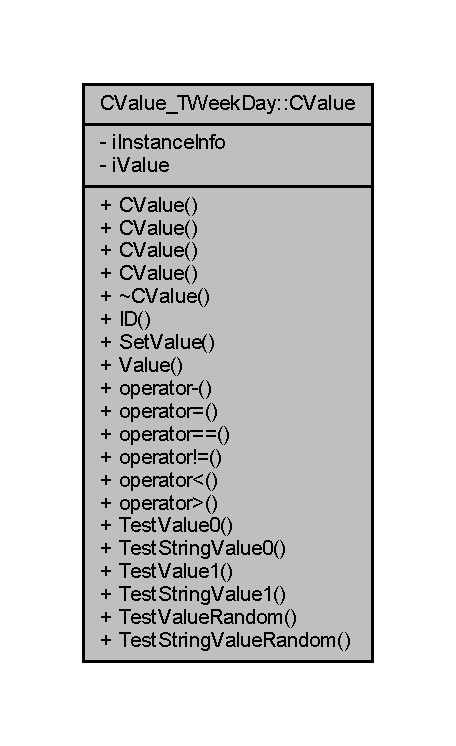
\includegraphics[width=219pt]{class_c_value___t_week_day_1_1_c_value__coll__graph}
\end{center}
\end{figure}
\subsection*{Public Member Functions}
\begin{DoxyCompactItemize}
\item 
\hyperlink{class_c_value___t_week_day_1_1_c_value_acea76df48114b736ed8002c542e59f0e}{C\+Value} ()
\begin{DoxyCompactList}\small\item\em Implicit c\textquotesingle{}tor. \end{DoxyCompactList}\item 
\hyperlink{class_c_value___t_week_day_1_1_c_value_a055e113aa1b4725dba3ddb8a7a986061}{C\+Value} (const enum \hyperlink{namespace_c_value___t_week_day_a6412f204509f223b789fb5f1a61a6124}{T\+Week\+Day} a\+Value)
\begin{DoxyCompactList}\small\item\em Conversion c\textquotesingle{}tor. \end{DoxyCompactList}\item 
\hyperlink{class_c_value___t_week_day_1_1_c_value_a758eb97770180f10addd1c597b13e6d2}{C\+Value} (const \hyperlink{class_c_value___t_week_day_1_1_c_value}{C\+Value} \&a\+Value)
\begin{DoxyCompactList}\small\item\em Copy c\textquotesingle{}tor. \end{DoxyCompactList}\item 
\hyperlink{class_c_value___t_week_day_1_1_c_value_a5f425476b8d7006138a270ba55c210b1}{C\+Value} (const char $\ast$a\+Str)
\begin{DoxyCompactList}\small\item\em String conversion c\textquotesingle{}tor. \end{DoxyCompactList}\item 
virtual \hyperlink{class_c_value___t_week_day_1_1_c_value_a2b588e6afc0801080a7c23291de5d964}{$\sim$\+C\+Value} ()
\begin{DoxyCompactList}\small\item\em Virtual d\textquotesingle{}tor. \end{DoxyCompactList}\item 
size\+\_\+t \hyperlink{class_c_value___t_week_day_1_1_c_value_ac1441867813d4c170f416b8fe5894324}{ID} () const
\begin{DoxyCompactList}\small\item\em ID getter. \end{DoxyCompactList}\item 
void \hyperlink{class_c_value___t_week_day_1_1_c_value_a3b2ee2ee229058d33770ec4787eed8a5}{Set\+Value} (const \hyperlink{namespace_c_value___t_week_day_a6412f204509f223b789fb5f1a61a6124}{T\+Week\+Day} a\+Value)
\begin{DoxyCompactList}\small\item\em Value setter. \end{DoxyCompactList}\item 
\hyperlink{namespace_c_value___t_week_day_a6412f204509f223b789fb5f1a61a6124}{T\+Week\+Day} \hyperlink{class_c_value___t_week_day_1_1_c_value_ae77674d9367e894d5627330076f585c4}{Value} () const
\begin{DoxyCompactList}\small\item\em Value getter. \end{DoxyCompactList}\item 
\hyperlink{class_c_value___t_week_day_1_1_c_value}{C\+Value} \hyperlink{class_c_value___t_week_day_1_1_c_value_a19635da2959641b25cd017f3a8edad38}{operator-\/} () const
\begin{DoxyCompactList}\small\item\em Complement operator. \end{DoxyCompactList}\item 
\hyperlink{class_c_value___t_week_day_1_1_c_value}{C\+Value} \& \hyperlink{class_c_value___t_week_day_1_1_c_value_a8b2de98efd431f204874ad7af5b6a712}{operator=} (const \hyperlink{class_c_value___t_week_day_1_1_c_value}{C\+Value} \&a\+Value)
\begin{DoxyCompactList}\small\item\em Assigment operator. \end{DoxyCompactList}\item 
bool \hyperlink{class_c_value___t_week_day_1_1_c_value_a24d761dc0cf9194eeff9750c92a8c6c5}{operator==} (const \hyperlink{class_c_value___t_week_day_1_1_c_value}{C\+Value} \&a\+Value) const
\begin{DoxyCompactList}\small\item\em Comparing by Value operator. \end{DoxyCompactList}\item 
bool \hyperlink{class_c_value___t_week_day_1_1_c_value_a22aa06908f1555784b3ff229c5a94da9}{operator!=} (const \hyperlink{class_c_value___t_week_day_1_1_c_value}{C\+Value} \&a\+Value) const
\begin{DoxyCompactList}\small\item\em Comparing by Value operator. \end{DoxyCompactList}\item 
bool \hyperlink{class_c_value___t_week_day_1_1_c_value_a8cbf6de4d8c42c14ce05ed46aa6ecb20}{operator$<$} (const \hyperlink{class_c_value___t_week_day_1_1_c_value}{C\+Value} \&a\+Value) const
\begin{DoxyCompactList}\small\item\em Comparing by Value operator. \end{DoxyCompactList}\item 
bool \hyperlink{class_c_value___t_week_day_1_1_c_value_ae5deb329e36bc2f814b39ca397199211}{operator$>$} (const \hyperlink{class_c_value___t_week_day_1_1_c_value}{C\+Value} \&a\+Value) const
\begin{DoxyCompactList}\small\item\em Comparing by Value operator. \end{DoxyCompactList}\end{DoxyCompactItemize}
\subsection*{Static Public Member Functions}
\begin{DoxyCompactItemize}
\item 
static \hyperlink{namespace_c_value___t_week_day_a6412f204509f223b789fb5f1a61a6124}{T\+Week\+Day} \hyperlink{class_c_value___t_week_day_1_1_c_value_ab2953ef7d3421ad741bed333e2188874}{Test\+Value0} ()
\begin{DoxyCompactList}\small\item\em First test value. \end{DoxyCompactList}\item 
static const char $\ast$ \hyperlink{class_c_value___t_week_day_1_1_c_value_ae28f515b823fa787ebc70b9498a0cb49}{Test\+String\+Value0} ()
\begin{DoxyCompactList}\small\item\em First test string value. \end{DoxyCompactList}\item 
static \hyperlink{namespace_c_value___t_week_day_a6412f204509f223b789fb5f1a61a6124}{T\+Week\+Day} \hyperlink{class_c_value___t_week_day_1_1_c_value_a8841fa6df3e84da037d9d34cc87a2581}{Test\+Value1} ()
\begin{DoxyCompactList}\small\item\em Second test value. \end{DoxyCompactList}\item 
static const char $\ast$ \hyperlink{class_c_value___t_week_day_1_1_c_value_a333999118ee2a849c35d2aa9aa6bc828}{Test\+String\+Value1} ()
\begin{DoxyCompactList}\small\item\em Second test string value. \end{DoxyCompactList}\item 
static \hyperlink{namespace_c_value___t_week_day_a6412f204509f223b789fb5f1a61a6124}{T\+Week\+Day} \hyperlink{class_c_value___t_week_day_1_1_c_value_a4d63e74d431ec7af57711f39ab703a8c}{Test\+Value\+Random} ()
\begin{DoxyCompactList}\small\item\em Random test value. \end{DoxyCompactList}\item 
static const char $\ast$ \hyperlink{class_c_value___t_week_day_1_1_c_value_a660e41950e476580acf00793fb43839a}{Test\+String\+Value\+Random} ()
\begin{DoxyCompactList}\small\item\em Random test string value. \end{DoxyCompactList}\end{DoxyCompactItemize}
\subsection*{Private Attributes}
\begin{DoxyCompactItemize}
\item 
Class\+Info$<$ \hyperlink{class_c_value___t_week_day_1_1_c_value}{C\+Value} $>$ \hyperlink{class_c_value___t_week_day_1_1_c_value_ad4482c30bcef137bae7669a2d7378cae}{i\+Instance\+Info}
\begin{DoxyCompactList}\small\item\em Instance of the class info for usage statistics. \end{DoxyCompactList}\item 
enum \hyperlink{namespace_c_value___t_week_day_a6412f204509f223b789fb5f1a61a6124}{T\+Week\+Day} \hyperlink{class_c_value___t_week_day_1_1_c_value_ad067d6e43b0204dc09f1177721891a75}{i\+Value}
\begin{DoxyCompactList}\small\item\em Encapsulated {\ttfamily enum} T\+Week\+Day value. \end{DoxyCompactList}\end{DoxyCompactItemize}
\subsection*{Friends}
\begin{DoxyCompactItemize}
\item 
std\+::ostream \& \hyperlink{class_c_value___t_week_day_1_1_c_value_a3d28097fae6bdd5a8146d9ab90f8b62f}{operator$<$$<$} (std\+::ostream \&a\+O\+Stream, const \hyperlink{class_c_value___t_week_day_1_1_c_value}{C\+Value} \&a\+Value)
\begin{DoxyCompactList}\small\item\em Output to the stream operator. ({\itshape serialization}) \end{DoxyCompactList}\item 
std\+::istream \& \hyperlink{class_c_value___t_week_day_1_1_c_value_aba05045ca890e398c1211784aebbc9ed}{operator$>$$>$} (std\+::istream \&a\+I\+Stream, \hyperlink{class_c_value___t_week_day_1_1_c_value}{C\+Value} \&a\+Value)
\begin{DoxyCompactList}\small\item\em Input from the stream operator. ({\itshape deserialization}) \end{DoxyCompactList}\end{DoxyCompactItemize}


\subsection{Detailed Description}
\hyperlink{class_c_value___t_week_day_1_1_c_value}{C\+Value} class ({\ttfamily T\+Week\+Day} variant) 

Definition of \hyperlink{class_c_value___t_week_day_1_1_c_value}{C\+Value} class ({\ttfamily T\+Week\+Day} variant). There is defined all common methods and attributes. 

Definition at line 68 of file C\+Value\+\_\+\+T\+Week\+Day.\+h.



\subsection{Constructor \& Destructor Documentation}
\mbox{\Hypertarget{class_c_value___t_week_day_1_1_c_value_acea76df48114b736ed8002c542e59f0e}\label{class_c_value___t_week_day_1_1_c_value_acea76df48114b736ed8002c542e59f0e}} 
\index{C\+Value\+\_\+\+T\+Week\+Day\+::\+C\+Value@{C\+Value\+\_\+\+T\+Week\+Day\+::\+C\+Value}!C\+Value@{C\+Value}}
\index{C\+Value@{C\+Value}!C\+Value\+\_\+\+T\+Week\+Day\+::\+C\+Value@{C\+Value\+\_\+\+T\+Week\+Day\+::\+C\+Value}}
\subsubsection{\texorpdfstring{C\+Value()}{CValue()}\hspace{0.1cm}{\footnotesize\ttfamily [1/4]}}
{\footnotesize\ttfamily C\+Value\+\_\+\+T\+Week\+Day\+::\+C\+Value\+::\+C\+Value (\begin{DoxyParamCaption}{ }\end{DoxyParamCaption})\hspace{0.3cm}{\ttfamily [inline]}}



Implicit c\textquotesingle{}tor. 

Value attributes is set to {\ttfamily E\+Monday}. 

Definition at line 78 of file C\+Value\+\_\+\+T\+Week\+Day.\+h.

\mbox{\Hypertarget{class_c_value___t_week_day_1_1_c_value_a055e113aa1b4725dba3ddb8a7a986061}\label{class_c_value___t_week_day_1_1_c_value_a055e113aa1b4725dba3ddb8a7a986061}} 
\index{C\+Value\+\_\+\+T\+Week\+Day\+::\+C\+Value@{C\+Value\+\_\+\+T\+Week\+Day\+::\+C\+Value}!C\+Value@{C\+Value}}
\index{C\+Value@{C\+Value}!C\+Value\+\_\+\+T\+Week\+Day\+::\+C\+Value@{C\+Value\+\_\+\+T\+Week\+Day\+::\+C\+Value}}
\subsubsection{\texorpdfstring{C\+Value()}{CValue()}\hspace{0.1cm}{\footnotesize\ttfamily [2/4]}}
{\footnotesize\ttfamily C\+Value\+\_\+\+T\+Week\+Day\+::\+C\+Value\+::\+C\+Value (\begin{DoxyParamCaption}\item[{const enum \hyperlink{namespace_c_value___t_week_day_a6412f204509f223b789fb5f1a61a6124}{T\+Week\+Day}}]{a\+Value }\end{DoxyParamCaption})\hspace{0.3cm}{\ttfamily [inline]}, {\ttfamily [explicit]}}



Conversion c\textquotesingle{}tor. 

Pointer attributes are initialised to the {\ttfamily this} value. 
\begin{DoxyParams}[1]{Parameters}
\mbox{\tt in}  & {\em a\+Value} & New T\+Week\+Day value \\
\hline
\end{DoxyParams}
\begin{DoxyAttention}{Attention}
Method generate {\ttfamily std\+::range\+\_\+error} exception if parameters {\ttfamily a\+Value} is out of the {\ttfamily enum} T\+Week\+Day range. 
\end{DoxyAttention}


Definition at line 86 of file C\+Value\+\_\+\+T\+Week\+Day.\+h.

\mbox{\Hypertarget{class_c_value___t_week_day_1_1_c_value_a758eb97770180f10addd1c597b13e6d2}\label{class_c_value___t_week_day_1_1_c_value_a758eb97770180f10addd1c597b13e6d2}} 
\index{C\+Value\+\_\+\+T\+Week\+Day\+::\+C\+Value@{C\+Value\+\_\+\+T\+Week\+Day\+::\+C\+Value}!C\+Value@{C\+Value}}
\index{C\+Value@{C\+Value}!C\+Value\+\_\+\+T\+Week\+Day\+::\+C\+Value@{C\+Value\+\_\+\+T\+Week\+Day\+::\+C\+Value}}
\subsubsection{\texorpdfstring{C\+Value()}{CValue()}\hspace{0.1cm}{\footnotesize\ttfamily [3/4]}}
{\footnotesize\ttfamily C\+Value\+\_\+\+T\+Week\+Day\+::\+C\+Value\+::\+C\+Value (\begin{DoxyParamCaption}\item[{const \hyperlink{class_c_value___t_week_day_1_1_c_value}{C\+Value} \&}]{a\+Value }\end{DoxyParamCaption})\hspace{0.3cm}{\ttfamily [inline]}}



Copy c\textquotesingle{}tor. 

Create new instance by copying only {\ttfamily i\+Value} parameter. 
\begin{DoxyParams}[1]{Parameters}
\mbox{\tt in}  & {\em a\+Value} & Original instance for copying \\
\hline
\end{DoxyParams}


Definition at line 93 of file C\+Value\+\_\+\+T\+Week\+Day.\+h.

\mbox{\Hypertarget{class_c_value___t_week_day_1_1_c_value_a5f425476b8d7006138a270ba55c210b1}\label{class_c_value___t_week_day_1_1_c_value_a5f425476b8d7006138a270ba55c210b1}} 
\index{C\+Value\+\_\+\+T\+Week\+Day\+::\+C\+Value@{C\+Value\+\_\+\+T\+Week\+Day\+::\+C\+Value}!C\+Value@{C\+Value}}
\index{C\+Value@{C\+Value}!C\+Value\+\_\+\+T\+Week\+Day\+::\+C\+Value@{C\+Value\+\_\+\+T\+Week\+Day\+::\+C\+Value}}
\subsubsection{\texorpdfstring{C\+Value()}{CValue()}\hspace{0.1cm}{\footnotesize\ttfamily [4/4]}}
{\footnotesize\ttfamily C\+Value\+\_\+\+T\+Week\+Day\+::\+C\+Value\+::\+C\+Value (\begin{DoxyParamCaption}\item[{const char $\ast$}]{a\+Str }\end{DoxyParamCaption})\hspace{0.3cm}{\ttfamily [inline]}, {\ttfamily [explicit]}}



String conversion c\textquotesingle{}tor. 

Create new instance from Value in the string. Pointer attributes are initialised to the {\ttfamily this} value. 
\begin{DoxyParams}[1]{Parameters}
\mbox{\tt in}  & {\em a\+Str} & Plain C string with string value convertable to the T\+Week\+Day value \\
\hline
\end{DoxyParams}


Definition at line 100 of file C\+Value\+\_\+\+T\+Week\+Day.\+h.

\mbox{\Hypertarget{class_c_value___t_week_day_1_1_c_value_a2b588e6afc0801080a7c23291de5d964}\label{class_c_value___t_week_day_1_1_c_value_a2b588e6afc0801080a7c23291de5d964}} 
\index{C\+Value\+\_\+\+T\+Week\+Day\+::\+C\+Value@{C\+Value\+\_\+\+T\+Week\+Day\+::\+C\+Value}!````~C\+Value@{$\sim$\+C\+Value}}
\index{````~C\+Value@{$\sim$\+C\+Value}!C\+Value\+\_\+\+T\+Week\+Day\+::\+C\+Value@{C\+Value\+\_\+\+T\+Week\+Day\+::\+C\+Value}}
\subsubsection{\texorpdfstring{$\sim$\+C\+Value()}{~CValue()}}
{\footnotesize\ttfamily virtual C\+Value\+\_\+\+T\+Week\+Day\+::\+C\+Value\+::$\sim$\+C\+Value (\begin{DoxyParamCaption}{ }\end{DoxyParamCaption})\hspace{0.3cm}{\ttfamily [inline]}, {\ttfamily [virtual]}}



Virtual d\textquotesingle{}tor. 



Definition at line 106 of file C\+Value\+\_\+\+T\+Week\+Day.\+h.



\subsection{Member Function Documentation}
\mbox{\Hypertarget{class_c_value___t_week_day_1_1_c_value_ac1441867813d4c170f416b8fe5894324}\label{class_c_value___t_week_day_1_1_c_value_ac1441867813d4c170f416b8fe5894324}} 
\index{C\+Value\+\_\+\+T\+Week\+Day\+::\+C\+Value@{C\+Value\+\_\+\+T\+Week\+Day\+::\+C\+Value}!ID@{ID}}
\index{ID@{ID}!C\+Value\+\_\+\+T\+Week\+Day\+::\+C\+Value@{C\+Value\+\_\+\+T\+Week\+Day\+::\+C\+Value}}
\subsubsection{\texorpdfstring{I\+D()}{ID()}}
{\footnotesize\ttfamily size\+\_\+t C\+Value\+\_\+\+T\+Week\+Day\+::\+C\+Value\+::\+ID (\begin{DoxyParamCaption}{ }\end{DoxyParamCaption}) const\hspace{0.3cm}{\ttfamily [inline]}}



ID getter. 

\begin{DoxyReturn}{Returns}
Unique instance ID 
\end{DoxyReturn}


Definition at line 113 of file C\+Value\+\_\+\+T\+Week\+Day.\+h.

\mbox{\Hypertarget{class_c_value___t_week_day_1_1_c_value_a22aa06908f1555784b3ff229c5a94da9}\label{class_c_value___t_week_day_1_1_c_value_a22aa06908f1555784b3ff229c5a94da9}} 
\index{C\+Value\+\_\+\+T\+Week\+Day\+::\+C\+Value@{C\+Value\+\_\+\+T\+Week\+Day\+::\+C\+Value}!operator"!=@{operator"!=}}
\index{operator"!=@{operator"!=}!C\+Value\+\_\+\+T\+Week\+Day\+::\+C\+Value@{C\+Value\+\_\+\+T\+Week\+Day\+::\+C\+Value}}
\subsubsection{\texorpdfstring{operator"!=()}{operator!=()}}
{\footnotesize\ttfamily bool C\+Value\+\_\+\+T\+Week\+Day\+::\+C\+Value\+::operator!= (\begin{DoxyParamCaption}\item[{const \hyperlink{class_c_value___t_week_day_1_1_c_value}{C\+Value} \&}]{a\+Value }\end{DoxyParamCaption}) const\hspace{0.3cm}{\ttfamily [inline]}}



Comparing by Value operator. 

\begin{DoxyReturn}{Returns}
Return {\ttfamily bool} result of comparation 
\end{DoxyReturn}


Definition at line 152 of file C\+Value\+\_\+\+T\+Week\+Day.\+h.

\mbox{\Hypertarget{class_c_value___t_week_day_1_1_c_value_a19635da2959641b25cd017f3a8edad38}\label{class_c_value___t_week_day_1_1_c_value_a19635da2959641b25cd017f3a8edad38}} 
\index{C\+Value\+\_\+\+T\+Week\+Day\+::\+C\+Value@{C\+Value\+\_\+\+T\+Week\+Day\+::\+C\+Value}!operator-\/@{operator-\/}}
\index{operator-\/@{operator-\/}!C\+Value\+\_\+\+T\+Week\+Day\+::\+C\+Value@{C\+Value\+\_\+\+T\+Week\+Day\+::\+C\+Value}}
\subsubsection{\texorpdfstring{operator-\/()}{operator-()}}
{\footnotesize\ttfamily \hyperlink{class_c_value___t_week_day_1_1_c_value}{C\+Value} C\+Value\+\_\+\+T\+Week\+Day\+::\+C\+Value\+::operator-\/ (\begin{DoxyParamCaption}{ }\end{DoxyParamCaption}) const\hspace{0.3cm}{\ttfamily [inline]}}



Complement operator. 

\begin{DoxyReturn}{Returns}
\hyperlink{class_c_value___t_week_day_1_1_c_value}{C\+Value} instance with complemented attribute Value. 
\end{DoxyReturn}


Definition at line 134 of file C\+Value\+\_\+\+T\+Week\+Day.\+h.

\mbox{\Hypertarget{class_c_value___t_week_day_1_1_c_value_a8cbf6de4d8c42c14ce05ed46aa6ecb20}\label{class_c_value___t_week_day_1_1_c_value_a8cbf6de4d8c42c14ce05ed46aa6ecb20}} 
\index{C\+Value\+\_\+\+T\+Week\+Day\+::\+C\+Value@{C\+Value\+\_\+\+T\+Week\+Day\+::\+C\+Value}!operator$<$@{operator$<$}}
\index{operator$<$@{operator$<$}!C\+Value\+\_\+\+T\+Week\+Day\+::\+C\+Value@{C\+Value\+\_\+\+T\+Week\+Day\+::\+C\+Value}}
\subsubsection{\texorpdfstring{operator$<$()}{operator<()}}
{\footnotesize\ttfamily bool C\+Value\+\_\+\+T\+Week\+Day\+::\+C\+Value\+::operator$<$ (\begin{DoxyParamCaption}\item[{const \hyperlink{class_c_value___t_week_day_1_1_c_value}{C\+Value} \&}]{a\+Value }\end{DoxyParamCaption}) const\hspace{0.3cm}{\ttfamily [inline]}}



Comparing by Value operator. 

\begin{DoxyReturn}{Returns}
Return {\ttfamily bool} result of comparation 
\end{DoxyReturn}


Definition at line 158 of file C\+Value\+\_\+\+T\+Week\+Day.\+h.

\mbox{\Hypertarget{class_c_value___t_week_day_1_1_c_value_a8b2de98efd431f204874ad7af5b6a712}\label{class_c_value___t_week_day_1_1_c_value_a8b2de98efd431f204874ad7af5b6a712}} 
\index{C\+Value\+\_\+\+T\+Week\+Day\+::\+C\+Value@{C\+Value\+\_\+\+T\+Week\+Day\+::\+C\+Value}!operator=@{operator=}}
\index{operator=@{operator=}!C\+Value\+\_\+\+T\+Week\+Day\+::\+C\+Value@{C\+Value\+\_\+\+T\+Week\+Day\+::\+C\+Value}}
\subsubsection{\texorpdfstring{operator=()}{operator=()}}
{\footnotesize\ttfamily \hyperlink{class_c_value___t_week_day_1_1_c_value}{C\+Value}\& C\+Value\+\_\+\+T\+Week\+Day\+::\+C\+Value\+::operator= (\begin{DoxyParamCaption}\item[{const \hyperlink{class_c_value___t_week_day_1_1_c_value}{C\+Value} \&}]{a\+Value }\end{DoxyParamCaption})\hspace{0.3cm}{\ttfamily [inline]}}



Assigment operator. 

\begin{DoxyReturn}{Returns}
\hyperlink{class_c_value___t_week_day_1_1_c_value}{C\+Value} instance with copied attribute Value. 
\end{DoxyReturn}


Definition at line 140 of file C\+Value\+\_\+\+T\+Week\+Day.\+h.

\mbox{\Hypertarget{class_c_value___t_week_day_1_1_c_value_a24d761dc0cf9194eeff9750c92a8c6c5}\label{class_c_value___t_week_day_1_1_c_value_a24d761dc0cf9194eeff9750c92a8c6c5}} 
\index{C\+Value\+\_\+\+T\+Week\+Day\+::\+C\+Value@{C\+Value\+\_\+\+T\+Week\+Day\+::\+C\+Value}!operator==@{operator==}}
\index{operator==@{operator==}!C\+Value\+\_\+\+T\+Week\+Day\+::\+C\+Value@{C\+Value\+\_\+\+T\+Week\+Day\+::\+C\+Value}}
\subsubsection{\texorpdfstring{operator==()}{operator==()}}
{\footnotesize\ttfamily bool C\+Value\+\_\+\+T\+Week\+Day\+::\+C\+Value\+::operator== (\begin{DoxyParamCaption}\item[{const \hyperlink{class_c_value___t_week_day_1_1_c_value}{C\+Value} \&}]{a\+Value }\end{DoxyParamCaption}) const\hspace{0.3cm}{\ttfamily [inline]}}



Comparing by Value operator. 

\begin{DoxyReturn}{Returns}
Return {\ttfamily bool} result of comparation 
\end{DoxyReturn}


Definition at line 146 of file C\+Value\+\_\+\+T\+Week\+Day.\+h.

\mbox{\Hypertarget{class_c_value___t_week_day_1_1_c_value_ae5deb329e36bc2f814b39ca397199211}\label{class_c_value___t_week_day_1_1_c_value_ae5deb329e36bc2f814b39ca397199211}} 
\index{C\+Value\+\_\+\+T\+Week\+Day\+::\+C\+Value@{C\+Value\+\_\+\+T\+Week\+Day\+::\+C\+Value}!operator$>$@{operator$>$}}
\index{operator$>$@{operator$>$}!C\+Value\+\_\+\+T\+Week\+Day\+::\+C\+Value@{C\+Value\+\_\+\+T\+Week\+Day\+::\+C\+Value}}
\subsubsection{\texorpdfstring{operator$>$()}{operator>()}}
{\footnotesize\ttfamily bool C\+Value\+\_\+\+T\+Week\+Day\+::\+C\+Value\+::operator$>$ (\begin{DoxyParamCaption}\item[{const \hyperlink{class_c_value___t_week_day_1_1_c_value}{C\+Value} \&}]{a\+Value }\end{DoxyParamCaption}) const\hspace{0.3cm}{\ttfamily [inline]}}



Comparing by Value operator. 

\begin{DoxyReturn}{Returns}
Return {\ttfamily bool} result of comparation 
\end{DoxyReturn}


Definition at line 164 of file C\+Value\+\_\+\+T\+Week\+Day.\+h.

\mbox{\Hypertarget{class_c_value___t_week_day_1_1_c_value_a3b2ee2ee229058d33770ec4787eed8a5}\label{class_c_value___t_week_day_1_1_c_value_a3b2ee2ee229058d33770ec4787eed8a5}} 
\index{C\+Value\+\_\+\+T\+Week\+Day\+::\+C\+Value@{C\+Value\+\_\+\+T\+Week\+Day\+::\+C\+Value}!Set\+Value@{Set\+Value}}
\index{Set\+Value@{Set\+Value}!C\+Value\+\_\+\+T\+Week\+Day\+::\+C\+Value@{C\+Value\+\_\+\+T\+Week\+Day\+::\+C\+Value}}
\subsubsection{\texorpdfstring{Set\+Value()}{SetValue()}}
{\footnotesize\ttfamily void C\+Value\+\_\+\+T\+Week\+Day\+::\+C\+Value\+::\+Set\+Value (\begin{DoxyParamCaption}\item[{const \hyperlink{namespace_c_value___t_week_day_a6412f204509f223b789fb5f1a61a6124}{T\+Week\+Day}}]{a\+Value }\end{DoxyParamCaption})\hspace{0.3cm}{\ttfamily [inline]}}



Value setter. 


\begin{DoxyParams}[1]{Parameters}
\mbox{\tt in}  & {\em a\+Value} & New Value \\
\hline
\end{DoxyParams}
\begin{DoxyAttention}{Attention}
Method generate {\ttfamily std\+::range\+\_\+error} exception if parameters {\ttfamily a\+Value} is out of the {\ttfamily enum} T\+Week\+Day range. 
\end{DoxyAttention}


Definition at line 121 of file C\+Value\+\_\+\+T\+Week\+Day.\+h.

\mbox{\Hypertarget{class_c_value___t_week_day_1_1_c_value_ae28f515b823fa787ebc70b9498a0cb49}\label{class_c_value___t_week_day_1_1_c_value_ae28f515b823fa787ebc70b9498a0cb49}} 
\index{C\+Value\+\_\+\+T\+Week\+Day\+::\+C\+Value@{C\+Value\+\_\+\+T\+Week\+Day\+::\+C\+Value}!Test\+String\+Value0@{Test\+String\+Value0}}
\index{Test\+String\+Value0@{Test\+String\+Value0}!C\+Value\+\_\+\+T\+Week\+Day\+::\+C\+Value@{C\+Value\+\_\+\+T\+Week\+Day\+::\+C\+Value}}
\subsubsection{\texorpdfstring{Test\+String\+Value0()}{TestStringValue0()}}
{\footnotesize\ttfamily static const char$\ast$ C\+Value\+\_\+\+T\+Week\+Day\+::\+C\+Value\+::\+Test\+String\+Value0 (\begin{DoxyParamCaption}{ }\end{DoxyParamCaption})\hspace{0.3cm}{\ttfamily [inline]}, {\ttfamily [static]}}



First test string value. 

\begin{DoxyReturn}{Returns}
Return string with T\+Week\+Day value (E\+Monday) 
\end{DoxyReturn}
\begin{DoxyNote}{Note}
Useful for automated testing of \hyperlink{class_c_value___t_week_day_1_1_c_value}{C\+Value} functionality 
\end{DoxyNote}


Definition at line 197 of file C\+Value\+\_\+\+T\+Week\+Day.\+h.

\mbox{\Hypertarget{class_c_value___t_week_day_1_1_c_value_a333999118ee2a849c35d2aa9aa6bc828}\label{class_c_value___t_week_day_1_1_c_value_a333999118ee2a849c35d2aa9aa6bc828}} 
\index{C\+Value\+\_\+\+T\+Week\+Day\+::\+C\+Value@{C\+Value\+\_\+\+T\+Week\+Day\+::\+C\+Value}!Test\+String\+Value1@{Test\+String\+Value1}}
\index{Test\+String\+Value1@{Test\+String\+Value1}!C\+Value\+\_\+\+T\+Week\+Day\+::\+C\+Value@{C\+Value\+\_\+\+T\+Week\+Day\+::\+C\+Value}}
\subsubsection{\texorpdfstring{Test\+String\+Value1()}{TestStringValue1()}}
{\footnotesize\ttfamily static const char$\ast$ C\+Value\+\_\+\+T\+Week\+Day\+::\+C\+Value\+::\+Test\+String\+Value1 (\begin{DoxyParamCaption}{ }\end{DoxyParamCaption})\hspace{0.3cm}{\ttfamily [inline]}, {\ttfamily [static]}}



Second test string value. 

\begin{DoxyReturn}{Returns}
Return string with T\+Week\+Day value (E\+Tuesday) 
\end{DoxyReturn}
\begin{DoxyNote}{Note}
Useful for automated testing of \hyperlink{class_c_value___t_week_day_1_1_c_value}{C\+Value} functionality 
\end{DoxyNote}


Definition at line 211 of file C\+Value\+\_\+\+T\+Week\+Day.\+h.

\mbox{\Hypertarget{class_c_value___t_week_day_1_1_c_value_a660e41950e476580acf00793fb43839a}\label{class_c_value___t_week_day_1_1_c_value_a660e41950e476580acf00793fb43839a}} 
\index{C\+Value\+\_\+\+T\+Week\+Day\+::\+C\+Value@{C\+Value\+\_\+\+T\+Week\+Day\+::\+C\+Value}!Test\+String\+Value\+Random@{Test\+String\+Value\+Random}}
\index{Test\+String\+Value\+Random@{Test\+String\+Value\+Random}!C\+Value\+\_\+\+T\+Week\+Day\+::\+C\+Value@{C\+Value\+\_\+\+T\+Week\+Day\+::\+C\+Value}}
\subsubsection{\texorpdfstring{Test\+String\+Value\+Random()}{TestStringValueRandom()}}
{\footnotesize\ttfamily static const char$\ast$ C\+Value\+\_\+\+T\+Week\+Day\+::\+C\+Value\+::\+Test\+String\+Value\+Random (\begin{DoxyParamCaption}{ }\end{DoxyParamCaption})\hspace{0.3cm}{\ttfamily [inline]}, {\ttfamily [static]}}



Random test string value. 

\begin{DoxyReturn}{Returns}
Return string with random T\+Week\+Day value 
\end{DoxyReturn}
\begin{DoxyNote}{Note}
Useful for automated testing of \hyperlink{class_c_value___t_week_day_1_1_c_value}{C\+Value} functionality 
\end{DoxyNote}


Definition at line 225 of file C\+Value\+\_\+\+T\+Week\+Day.\+h.

\mbox{\Hypertarget{class_c_value___t_week_day_1_1_c_value_ab2953ef7d3421ad741bed333e2188874}\label{class_c_value___t_week_day_1_1_c_value_ab2953ef7d3421ad741bed333e2188874}} 
\index{C\+Value\+\_\+\+T\+Week\+Day\+::\+C\+Value@{C\+Value\+\_\+\+T\+Week\+Day\+::\+C\+Value}!Test\+Value0@{Test\+Value0}}
\index{Test\+Value0@{Test\+Value0}!C\+Value\+\_\+\+T\+Week\+Day\+::\+C\+Value@{C\+Value\+\_\+\+T\+Week\+Day\+::\+C\+Value}}
\subsubsection{\texorpdfstring{Test\+Value0()}{TestValue0()}}
{\footnotesize\ttfamily static \hyperlink{namespace_c_value___t_week_day_a6412f204509f223b789fb5f1a61a6124}{T\+Week\+Day} C\+Value\+\_\+\+T\+Week\+Day\+::\+C\+Value\+::\+Test\+Value0 (\begin{DoxyParamCaption}{ }\end{DoxyParamCaption})\hspace{0.3cm}{\ttfamily [inline]}, {\ttfamily [static]}}



First test value. 

\begin{DoxyReturn}{Returns}
Return T\+Week\+Day value (E\+Monday) 
\end{DoxyReturn}
\begin{DoxyNote}{Note}
Useful for automated testing of \hyperlink{class_c_value___t_week_day_1_1_c_value}{C\+Value} functionality 
\end{DoxyNote}


Definition at line 190 of file C\+Value\+\_\+\+T\+Week\+Day.\+h.

\mbox{\Hypertarget{class_c_value___t_week_day_1_1_c_value_a8841fa6df3e84da037d9d34cc87a2581}\label{class_c_value___t_week_day_1_1_c_value_a8841fa6df3e84da037d9d34cc87a2581}} 
\index{C\+Value\+\_\+\+T\+Week\+Day\+::\+C\+Value@{C\+Value\+\_\+\+T\+Week\+Day\+::\+C\+Value}!Test\+Value1@{Test\+Value1}}
\index{Test\+Value1@{Test\+Value1}!C\+Value\+\_\+\+T\+Week\+Day\+::\+C\+Value@{C\+Value\+\_\+\+T\+Week\+Day\+::\+C\+Value}}
\subsubsection{\texorpdfstring{Test\+Value1()}{TestValue1()}}
{\footnotesize\ttfamily static \hyperlink{namespace_c_value___t_week_day_a6412f204509f223b789fb5f1a61a6124}{T\+Week\+Day} C\+Value\+\_\+\+T\+Week\+Day\+::\+C\+Value\+::\+Test\+Value1 (\begin{DoxyParamCaption}{ }\end{DoxyParamCaption})\hspace{0.3cm}{\ttfamily [inline]}, {\ttfamily [static]}}



Second test value. 

\begin{DoxyReturn}{Returns}
Return T\+Week\+Day value (E\+Tuesday) 
\end{DoxyReturn}
\begin{DoxyNote}{Note}
Useful for automated testing of \hyperlink{class_c_value___t_week_day_1_1_c_value}{C\+Value} functionality 
\end{DoxyNote}


Definition at line 204 of file C\+Value\+\_\+\+T\+Week\+Day.\+h.

\mbox{\Hypertarget{class_c_value___t_week_day_1_1_c_value_a4d63e74d431ec7af57711f39ab703a8c}\label{class_c_value___t_week_day_1_1_c_value_a4d63e74d431ec7af57711f39ab703a8c}} 
\index{C\+Value\+\_\+\+T\+Week\+Day\+::\+C\+Value@{C\+Value\+\_\+\+T\+Week\+Day\+::\+C\+Value}!Test\+Value\+Random@{Test\+Value\+Random}}
\index{Test\+Value\+Random@{Test\+Value\+Random}!C\+Value\+\_\+\+T\+Week\+Day\+::\+C\+Value@{C\+Value\+\_\+\+T\+Week\+Day\+::\+C\+Value}}
\subsubsection{\texorpdfstring{Test\+Value\+Random()}{TestValueRandom()}}
{\footnotesize\ttfamily static \hyperlink{namespace_c_value___t_week_day_a6412f204509f223b789fb5f1a61a6124}{T\+Week\+Day} C\+Value\+\_\+\+T\+Week\+Day\+::\+C\+Value\+::\+Test\+Value\+Random (\begin{DoxyParamCaption}{ }\end{DoxyParamCaption})\hspace{0.3cm}{\ttfamily [inline]}, {\ttfamily [static]}}



Random test value. 

\begin{DoxyReturn}{Returns}
Return random T\+Week\+Day value 
\end{DoxyReturn}
\begin{DoxyNote}{Note}
Useful for automated testing of \hyperlink{class_c_value___t_week_day_1_1_c_value}{C\+Value} functionality 
\end{DoxyNote}


Definition at line 218 of file C\+Value\+\_\+\+T\+Week\+Day.\+h.

\mbox{\Hypertarget{class_c_value___t_week_day_1_1_c_value_ae77674d9367e894d5627330076f585c4}\label{class_c_value___t_week_day_1_1_c_value_ae77674d9367e894d5627330076f585c4}} 
\index{C\+Value\+\_\+\+T\+Week\+Day\+::\+C\+Value@{C\+Value\+\_\+\+T\+Week\+Day\+::\+C\+Value}!Value@{Value}}
\index{Value@{Value}!C\+Value\+\_\+\+T\+Week\+Day\+::\+C\+Value@{C\+Value\+\_\+\+T\+Week\+Day\+::\+C\+Value}}
\subsubsection{\texorpdfstring{Value()}{Value()}}
{\footnotesize\ttfamily \hyperlink{namespace_c_value___t_week_day_a6412f204509f223b789fb5f1a61a6124}{T\+Week\+Day} C\+Value\+\_\+\+T\+Week\+Day\+::\+C\+Value\+::\+Value (\begin{DoxyParamCaption}{ }\end{DoxyParamCaption}) const\hspace{0.3cm}{\ttfamily [inline]}}



Value getter. 

\begin{DoxyReturn}{Returns}
Actual {\ttfamily bool} {\ttfamily Value} 
\end{DoxyReturn}


Definition at line 127 of file C\+Value\+\_\+\+T\+Week\+Day.\+h.



\subsection{Friends And Related Function Documentation}
\mbox{\Hypertarget{class_c_value___t_week_day_1_1_c_value_a3d28097fae6bdd5a8146d9ab90f8b62f}\label{class_c_value___t_week_day_1_1_c_value_a3d28097fae6bdd5a8146d9ab90f8b62f}} 
\index{C\+Value\+\_\+\+T\+Week\+Day\+::\+C\+Value@{C\+Value\+\_\+\+T\+Week\+Day\+::\+C\+Value}!operator$<$$<$@{operator$<$$<$}}
\index{operator$<$$<$@{operator$<$$<$}!C\+Value\+\_\+\+T\+Week\+Day\+::\+C\+Value@{C\+Value\+\_\+\+T\+Week\+Day\+::\+C\+Value}}
\subsubsection{\texorpdfstring{operator$<$$<$}{operator<<}}
{\footnotesize\ttfamily std\+::ostream\& operator$<$$<$ (\begin{DoxyParamCaption}\item[{std\+::ostream \&}]{a\+O\+Stream,  }\item[{const \hyperlink{class_c_value___t_week_day_1_1_c_value}{C\+Value} \&}]{a\+Value }\end{DoxyParamCaption})\hspace{0.3cm}{\ttfamily [friend]}}



Output to the stream operator. ({\itshape serialization}) 


\begin{DoxyParams}[1]{Parameters}
\mbox{\tt in}  & {\em a\+O\+Stream} & Output stream \\
\hline
\mbox{\tt in}  & {\em a\+Value} & Serialized instantion of \hyperlink{class_c_value___t_week_day_1_1_c_value}{C\+Value} \\
\hline
\end{DoxyParams}
\begin{DoxyReturn}{Returns}
Return {\ttfamily std\+::ostream} with serialized Value 
\end{DoxyReturn}


Definition at line 172 of file C\+Value\+\_\+\+T\+Week\+Day.\+h.

\mbox{\Hypertarget{class_c_value___t_week_day_1_1_c_value_aba05045ca890e398c1211784aebbc9ed}\label{class_c_value___t_week_day_1_1_c_value_aba05045ca890e398c1211784aebbc9ed}} 
\index{C\+Value\+\_\+\+T\+Week\+Day\+::\+C\+Value@{C\+Value\+\_\+\+T\+Week\+Day\+::\+C\+Value}!operator$>$$>$@{operator$>$$>$}}
\index{operator$>$$>$@{operator$>$$>$}!C\+Value\+\_\+\+T\+Week\+Day\+::\+C\+Value@{C\+Value\+\_\+\+T\+Week\+Day\+::\+C\+Value}}
\subsubsection{\texorpdfstring{operator$>$$>$}{operator>>}}
{\footnotesize\ttfamily std\+::istream\& operator$>$$>$ (\begin{DoxyParamCaption}\item[{std\+::istream \&}]{a\+I\+Stream,  }\item[{\hyperlink{class_c_value___t_week_day_1_1_c_value}{C\+Value} \&}]{a\+Value }\end{DoxyParamCaption})\hspace{0.3cm}{\ttfamily [friend]}}



Input from the stream operator. ({\itshape deserialization}) 


\begin{DoxyParams}[1]{Parameters}
\mbox{\tt in}  & {\em a\+I\+Stream} & Input stream \\
\hline
\mbox{\tt out}  & {\em a\+Value} & Place for deserialized instantion of \hyperlink{class_c_value___t_week_day_1_1_c_value}{C\+Value} \\
\hline
\end{DoxyParams}
\begin{DoxyReturn}{Returns}
Return rest of {\ttfamily std\+::istream} 
\end{DoxyReturn}


Definition at line 180 of file C\+Value\+\_\+\+T\+Week\+Day.\+h.



\subsection{Member Data Documentation}
\mbox{\Hypertarget{class_c_value___t_week_day_1_1_c_value_ad4482c30bcef137bae7669a2d7378cae}\label{class_c_value___t_week_day_1_1_c_value_ad4482c30bcef137bae7669a2d7378cae}} 
\index{C\+Value\+\_\+\+T\+Week\+Day\+::\+C\+Value@{C\+Value\+\_\+\+T\+Week\+Day\+::\+C\+Value}!i\+Instance\+Info@{i\+Instance\+Info}}
\index{i\+Instance\+Info@{i\+Instance\+Info}!C\+Value\+\_\+\+T\+Week\+Day\+::\+C\+Value@{C\+Value\+\_\+\+T\+Week\+Day\+::\+C\+Value}}
\subsubsection{\texorpdfstring{i\+Instance\+Info}{iInstanceInfo}}
{\footnotesize\ttfamily Class\+Info$<$\hyperlink{class_c_value___t_week_day_1_1_c_value}{C\+Value}$>$ C\+Value\+\_\+\+T\+Week\+Day\+::\+C\+Value\+::i\+Instance\+Info\hspace{0.3cm}{\ttfamily [private]}}



Instance of the class info for usage statistics. 



Definition at line 70 of file C\+Value\+\_\+\+T\+Week\+Day.\+h.

\mbox{\Hypertarget{class_c_value___t_week_day_1_1_c_value_ad067d6e43b0204dc09f1177721891a75}\label{class_c_value___t_week_day_1_1_c_value_ad067d6e43b0204dc09f1177721891a75}} 
\index{C\+Value\+\_\+\+T\+Week\+Day\+::\+C\+Value@{C\+Value\+\_\+\+T\+Week\+Day\+::\+C\+Value}!i\+Value@{i\+Value}}
\index{i\+Value@{i\+Value}!C\+Value\+\_\+\+T\+Week\+Day\+::\+C\+Value@{C\+Value\+\_\+\+T\+Week\+Day\+::\+C\+Value}}
\subsubsection{\texorpdfstring{i\+Value}{iValue}}
{\footnotesize\ttfamily enum \hyperlink{namespace_c_value___t_week_day_a6412f204509f223b789fb5f1a61a6124}{T\+Week\+Day} C\+Value\+\_\+\+T\+Week\+Day\+::\+C\+Value\+::i\+Value\hspace{0.3cm}{\ttfamily [private]}}



Encapsulated {\ttfamily enum} T\+Week\+Day value. 



Definition at line 71 of file C\+Value\+\_\+\+T\+Week\+Day.\+h.



The documentation for this class was generated from the following file\+:\begin{DoxyCompactItemize}
\item 
\hyperlink{_c_value___t_week_day_8h}{C\+Value\+\_\+\+T\+Week\+Day.\+h}\end{DoxyCompactItemize}

\hypertarget{struct_c_hash_map_1_1_t_bucket}{}\section{C\+Hash\+Map\+:\+:T\+Bucket Struct Reference}
\label{struct_c_hash_map_1_1_t_bucket}\index{C\+Hash\+Map\+::\+T\+Bucket@{C\+Hash\+Map\+::\+T\+Bucket}}


\hyperlink{struct_c_hash_map_1_1_t_bucket}{T\+Bucket} structure definition.  




Collaboration diagram for C\+Hash\+Map\+:\+:T\+Bucket\+:\nopagebreak
\begin{figure}[H]
\begin{center}
\leavevmode
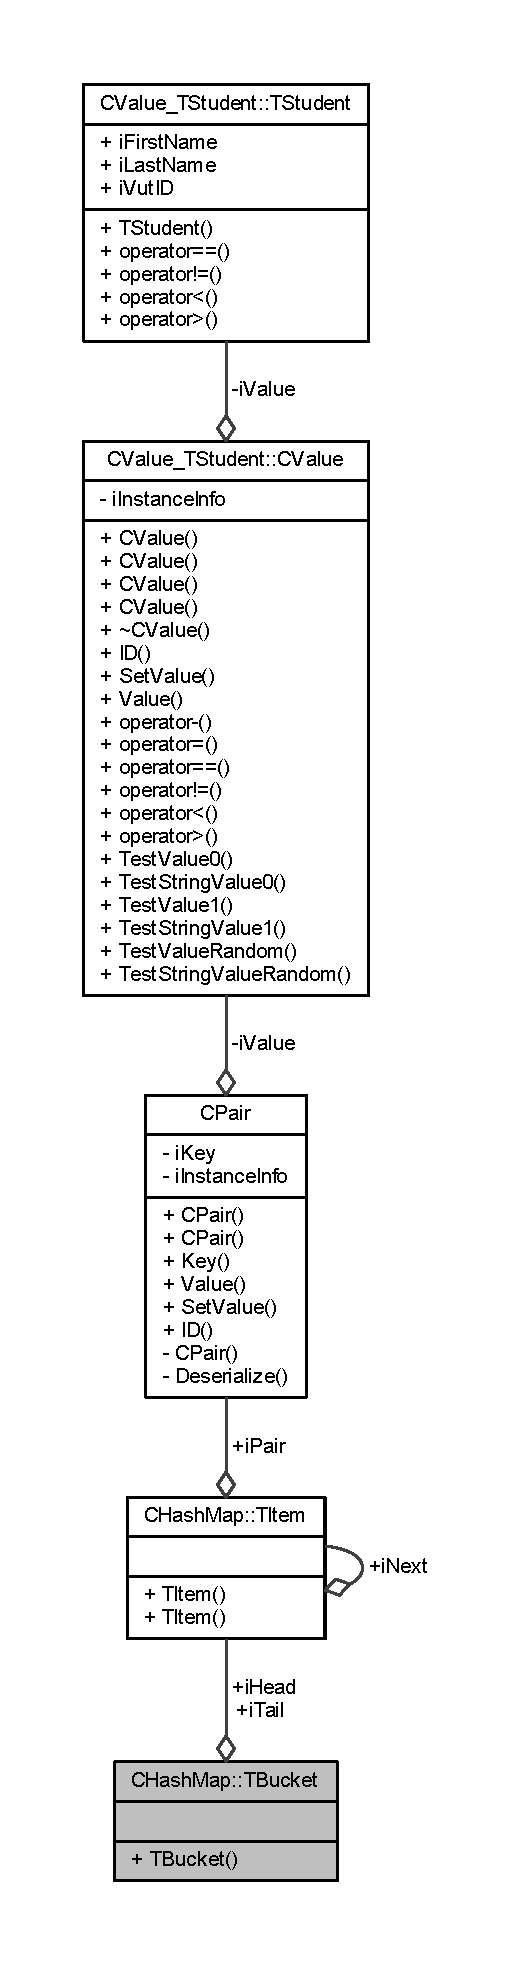
\includegraphics[height=550pt]{struct_c_hash_map_1_1_t_bucket__coll__graph}
\end{center}
\end{figure}
\subsection*{Public Member Functions}
\begin{DoxyCompactItemize}
\item 
\hyperlink{struct_c_hash_map_1_1_t_bucket_a8215764debe089e414b6f79d351cb4e2}{T\+Bucket} (\hyperlink{struct_c_hash_map_1_1_t_item}{T\+Item} $\ast$a\+Head=nullptr, \hyperlink{struct_c_hash_map_1_1_t_item}{T\+Item} $\ast$a\+Tail=nullptr)
\begin{DoxyCompactList}\small\item\em Implicit and Conversion c\textquotesingle{}tor for handy initialization of \hyperlink{struct_c_hash_map_1_1_t_bucket}{T\+Bucket} instance. \end{DoxyCompactList}\end{DoxyCompactItemize}
\subsection*{Public Attributes}
\begin{DoxyCompactItemize}
\item 
\hyperlink{struct_c_hash_map_1_1_t_item}{T\+Item} $\ast$ \hyperlink{struct_c_hash_map_1_1_t_bucket_a03a10c5ce912fd09137778c3454e7d77}{i\+Head}
\begin{DoxyCompactList}\small\item\em Pointer to first item in the linked list. \end{DoxyCompactList}\item 
\hyperlink{struct_c_hash_map_1_1_t_item}{T\+Item} $\ast$ \hyperlink{struct_c_hash_map_1_1_t_bucket_a1b8b634924907ed251a58eee989d577a}{i\+Tail}
\begin{DoxyCompactList}\small\item\em Pointer to last item in the linked list. \end{DoxyCompactList}\end{DoxyCompactItemize}


\subsection{Detailed Description}
\hyperlink{struct_c_hash_map_1_1_t_bucket}{T\+Bucket} structure definition. 

Definition of \hyperlink{struct_c_hash_map_1_1_t_bucket}{T\+Bucket} struct which is used for storing head and tail pointers to item in the linked list 

Definition at line 89 of file C\+Hash\+Map.\+h.



\subsection{Constructor \& Destructor Documentation}
\mbox{\Hypertarget{struct_c_hash_map_1_1_t_bucket_a8215764debe089e414b6f79d351cb4e2}\label{struct_c_hash_map_1_1_t_bucket_a8215764debe089e414b6f79d351cb4e2}} 
\index{C\+Hash\+Map\+::\+T\+Bucket@{C\+Hash\+Map\+::\+T\+Bucket}!T\+Bucket@{T\+Bucket}}
\index{T\+Bucket@{T\+Bucket}!C\+Hash\+Map\+::\+T\+Bucket@{C\+Hash\+Map\+::\+T\+Bucket}}
\subsubsection{\texorpdfstring{T\+Bucket()}{TBucket()}}
{\footnotesize\ttfamily C\+Hash\+Map\+::\+T\+Bucket\+::\+T\+Bucket (\begin{DoxyParamCaption}\item[{\hyperlink{struct_c_hash_map_1_1_t_item}{T\+Item} $\ast$}]{a\+Head = {\ttfamily nullptr},  }\item[{\hyperlink{struct_c_hash_map_1_1_t_item}{T\+Item} $\ast$}]{a\+Tail = {\ttfamily nullptr} }\end{DoxyParamCaption})\hspace{0.3cm}{\ttfamily [inline]}}



Implicit and Conversion c\textquotesingle{}tor for handy initialization of \hyperlink{struct_c_hash_map_1_1_t_bucket}{T\+Bucket} instance. 


\begin{DoxyParams}[1]{Parameters}
\mbox{\tt in}  & {\em a\+Head} & Pointer to the first item in the linked list (can be ommited) \\
\hline
\mbox{\tt in}  & {\em a\+Tail} & Pointer to the last item in the linked list (can be ommited) \\
\hline
\end{DoxyParams}


Definition at line 98 of file C\+Hash\+Map.\+h.



\subsection{Member Data Documentation}
\mbox{\Hypertarget{struct_c_hash_map_1_1_t_bucket_a03a10c5ce912fd09137778c3454e7d77}\label{struct_c_hash_map_1_1_t_bucket_a03a10c5ce912fd09137778c3454e7d77}} 
\index{C\+Hash\+Map\+::\+T\+Bucket@{C\+Hash\+Map\+::\+T\+Bucket}!i\+Head@{i\+Head}}
\index{i\+Head@{i\+Head}!C\+Hash\+Map\+::\+T\+Bucket@{C\+Hash\+Map\+::\+T\+Bucket}}
\subsubsection{\texorpdfstring{i\+Head}{iHead}}
{\footnotesize\ttfamily \hyperlink{struct_c_hash_map_1_1_t_item}{T\+Item}$\ast$ C\+Hash\+Map\+::\+T\+Bucket\+::i\+Head}



Pointer to first item in the linked list. 



Definition at line 91 of file C\+Hash\+Map.\+h.

\mbox{\Hypertarget{struct_c_hash_map_1_1_t_bucket_a1b8b634924907ed251a58eee989d577a}\label{struct_c_hash_map_1_1_t_bucket_a1b8b634924907ed251a58eee989d577a}} 
\index{C\+Hash\+Map\+::\+T\+Bucket@{C\+Hash\+Map\+::\+T\+Bucket}!i\+Tail@{i\+Tail}}
\index{i\+Tail@{i\+Tail}!C\+Hash\+Map\+::\+T\+Bucket@{C\+Hash\+Map\+::\+T\+Bucket}}
\subsubsection{\texorpdfstring{i\+Tail}{iTail}}
{\footnotesize\ttfamily \hyperlink{struct_c_hash_map_1_1_t_item}{T\+Item}$\ast$ C\+Hash\+Map\+::\+T\+Bucket\+::i\+Tail}



Pointer to last item in the linked list. 



Definition at line 92 of file C\+Hash\+Map.\+h.



The documentation for this struct was generated from the following file\+:\begin{DoxyCompactItemize}
\item 
\hyperlink{_c_hash_map_8h}{C\+Hash\+Map.\+h}\end{DoxyCompactItemize}

\hypertarget{struct_c_hash_map_1_1_t_item}{}\section{C\+Hash\+Map\+:\+:T\+Item Struct Reference}
\label{struct_c_hash_map_1_1_t_item}\index{C\+Hash\+Map\+::\+T\+Item@{C\+Hash\+Map\+::\+T\+Item}}


\hyperlink{struct_c_hash_map_1_1_t_item}{T\+Item} structure definiton.  




Collaboration diagram for C\+Hash\+Map\+:\+:T\+Item\+:\nopagebreak
\begin{figure}[H]
\begin{center}
\leavevmode
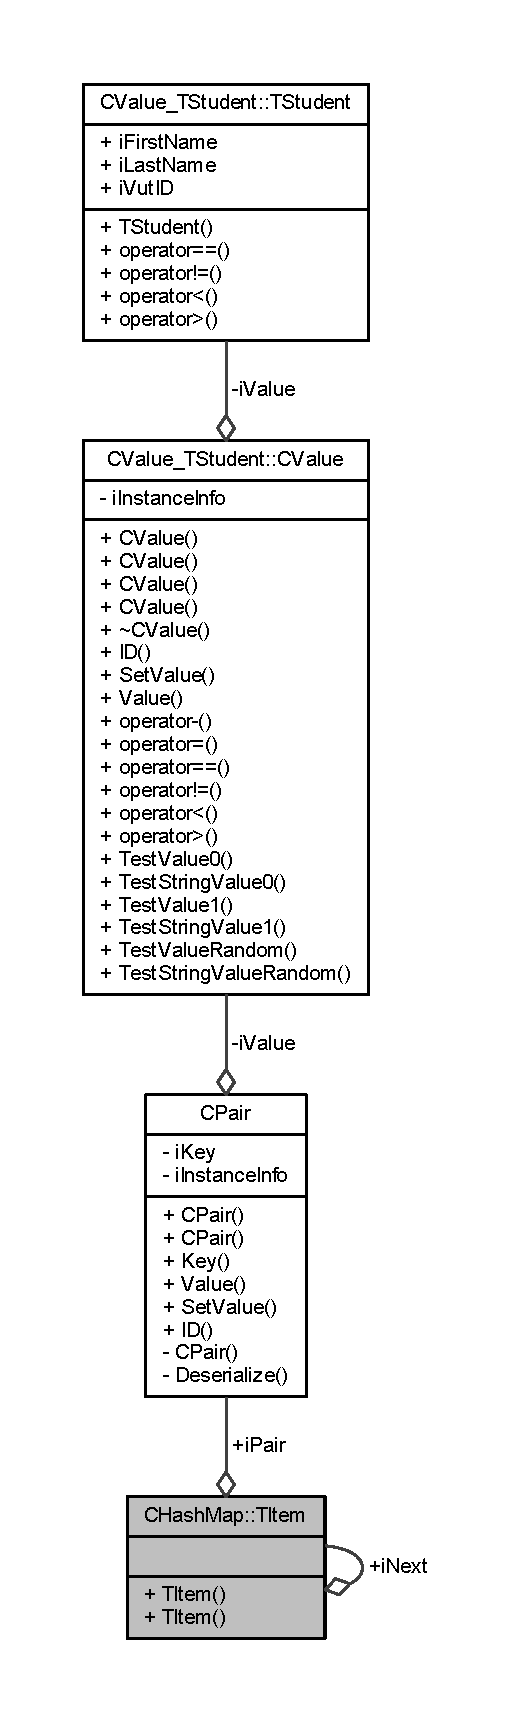
\includegraphics[height=550pt]{struct_c_hash_map_1_1_t_item__coll__graph}
\end{center}
\end{figure}
\subsection*{Public Member Functions}
\begin{DoxyCompactItemize}
\item 
\hyperlink{struct_c_hash_map_1_1_t_item_a7dce7ef1ebf814b1f2e8abb22e6bbf3a}{T\+Item} (const \hyperlink{class_c_pair}{C\+Pair} \&a\+Pair, \hyperlink{struct_c_hash_map_1_1_t_item}{T\+Item} $\ast$a\+Next=nullptr)
\begin{DoxyCompactList}\small\item\em Copy and conversion c\textquotesingle{}tor for handy initialization of \hyperlink{struct_c_hash_map_1_1_t_item}{T\+Item} instance. \end{DoxyCompactList}\item 
\hyperlink{struct_c_hash_map_1_1_t_item_ab8e18615d2569ae7a1ff57ff982ceb7d}{T\+Item} (\hyperlink{class_c_pair}{C\+Pair} \&\&a\+Pair, \hyperlink{struct_c_hash_map_1_1_t_item}{T\+Item} $\ast$a\+Next=nullptr)
\begin{DoxyCompactList}\small\item\em Move and conversion c\textquotesingle{}tor for handy initialization of \hyperlink{struct_c_hash_map_1_1_t_item}{T\+Item} instance. \end{DoxyCompactList}\end{DoxyCompactItemize}
\subsection*{Public Attributes}
\begin{DoxyCompactItemize}
\item 
\hyperlink{class_c_pair}{C\+Pair} \hyperlink{struct_c_hash_map_1_1_t_item_a9b832f579f07c1011ef58d89a589470a}{i\+Pair}
\begin{DoxyCompactList}\small\item\em Pair value. \end{DoxyCompactList}\item 
\hyperlink{struct_c_hash_map_1_1_t_item}{T\+Item} $\ast$ \hyperlink{struct_c_hash_map_1_1_t_item_a7d4fed6cab5e5e567fddc934a8ace1f7}{i\+Next}
\begin{DoxyCompactList}\small\item\em Pointer to the next item in the linked list. \end{DoxyCompactList}\end{DoxyCompactItemize}


\subsection{Detailed Description}
\hyperlink{struct_c_hash_map_1_1_t_item}{T\+Item} structure definiton. 

Definition of \hyperlink{struct_c_hash_map_1_1_t_item}{T\+Item} struct which is used as item in the linked list 

Definition at line 49 of file C\+Hash\+Map.\+h.



\subsection{Constructor \& Destructor Documentation}
\mbox{\Hypertarget{struct_c_hash_map_1_1_t_item_a7dce7ef1ebf814b1f2e8abb22e6bbf3a}\label{struct_c_hash_map_1_1_t_item_a7dce7ef1ebf814b1f2e8abb22e6bbf3a}} 
\index{C\+Hash\+Map\+::\+T\+Item@{C\+Hash\+Map\+::\+T\+Item}!T\+Item@{T\+Item}}
\index{T\+Item@{T\+Item}!C\+Hash\+Map\+::\+T\+Item@{C\+Hash\+Map\+::\+T\+Item}}
\subsubsection{\texorpdfstring{T\+Item()}{TItem()}\hspace{0.1cm}{\footnotesize\ttfamily [1/2]}}
{\footnotesize\ttfamily C\+Hash\+Map\+::\+T\+Item\+::\+T\+Item (\begin{DoxyParamCaption}\item[{const \hyperlink{class_c_pair}{C\+Pair} \&}]{a\+Pair,  }\item[{\hyperlink{struct_c_hash_map_1_1_t_item}{T\+Item} $\ast$}]{a\+Next = {\ttfamily nullptr} }\end{DoxyParamCaption})\hspace{0.3cm}{\ttfamily [inline]}}



Copy and conversion c\textquotesingle{}tor for handy initialization of \hyperlink{struct_c_hash_map_1_1_t_item}{T\+Item} instance. 


\begin{DoxyParams}[1]{Parameters}
\mbox{\tt in}  & {\em a\+Pair} & Pair (key, value) \\
\hline
\mbox{\tt in}  & {\em a\+Next} & Pointer to the next item in the linked list (can be ommited) \\
\hline
\end{DoxyParams}


Definition at line 65 of file C\+Hash\+Map.\+h.

\mbox{\Hypertarget{struct_c_hash_map_1_1_t_item_ab8e18615d2569ae7a1ff57ff982ceb7d}\label{struct_c_hash_map_1_1_t_item_ab8e18615d2569ae7a1ff57ff982ceb7d}} 
\index{C\+Hash\+Map\+::\+T\+Item@{C\+Hash\+Map\+::\+T\+Item}!T\+Item@{T\+Item}}
\index{T\+Item@{T\+Item}!C\+Hash\+Map\+::\+T\+Item@{C\+Hash\+Map\+::\+T\+Item}}
\subsubsection{\texorpdfstring{T\+Item()}{TItem()}\hspace{0.1cm}{\footnotesize\ttfamily [2/2]}}
{\footnotesize\ttfamily C\+Hash\+Map\+::\+T\+Item\+::\+T\+Item (\begin{DoxyParamCaption}\item[{\hyperlink{class_c_pair}{C\+Pair} \&\&}]{a\+Pair,  }\item[{\hyperlink{struct_c_hash_map_1_1_t_item}{T\+Item} $\ast$}]{a\+Next = {\ttfamily nullptr} }\end{DoxyParamCaption})\hspace{0.3cm}{\ttfamily [inline]}}



Move and conversion c\textquotesingle{}tor for handy initialization of \hyperlink{struct_c_hash_map_1_1_t_item}{T\+Item} instance. 


\begin{DoxyParams}[1]{Parameters}
\mbox{\tt in}  & {\em a\+Pair} & Pair (key, value) \\
\hline
\mbox{\tt in}  & {\em a\+Next} & Pointer to the next item in the linked list (can be ommited) \\
\hline
\end{DoxyParams}


Definition at line 78 of file C\+Hash\+Map.\+h.



\subsection{Member Data Documentation}
\mbox{\Hypertarget{struct_c_hash_map_1_1_t_item_a7d4fed6cab5e5e567fddc934a8ace1f7}\label{struct_c_hash_map_1_1_t_item_a7d4fed6cab5e5e567fddc934a8ace1f7}} 
\index{C\+Hash\+Map\+::\+T\+Item@{C\+Hash\+Map\+::\+T\+Item}!i\+Next@{i\+Next}}
\index{i\+Next@{i\+Next}!C\+Hash\+Map\+::\+T\+Item@{C\+Hash\+Map\+::\+T\+Item}}
\subsubsection{\texorpdfstring{i\+Next}{iNext}}
{\footnotesize\ttfamily \hyperlink{struct_c_hash_map_1_1_t_item}{T\+Item}$\ast$ C\+Hash\+Map\+::\+T\+Item\+::i\+Next}



Pointer to the next item in the linked list. 



Definition at line 54 of file C\+Hash\+Map.\+h.

\mbox{\Hypertarget{struct_c_hash_map_1_1_t_item_a9b832f579f07c1011ef58d89a589470a}\label{struct_c_hash_map_1_1_t_item_a9b832f579f07c1011ef58d89a589470a}} 
\index{C\+Hash\+Map\+::\+T\+Item@{C\+Hash\+Map\+::\+T\+Item}!i\+Pair@{i\+Pair}}
\index{i\+Pair@{i\+Pair}!C\+Hash\+Map\+::\+T\+Item@{C\+Hash\+Map\+::\+T\+Item}}
\subsubsection{\texorpdfstring{i\+Pair}{iPair}}
{\footnotesize\ttfamily \hyperlink{class_c_pair}{C\+Pair} C\+Hash\+Map\+::\+T\+Item\+::i\+Pair}



Pair value. 



Definition at line 53 of file C\+Hash\+Map.\+h.



The documentation for this struct was generated from the following file\+:\begin{DoxyCompactItemize}
\item 
\hyperlink{_c_hash_map_8h}{C\+Hash\+Map.\+h}\end{DoxyCompactItemize}

\hypertarget{struct_c_value___t_student_1_1_t_student}{}\section{C\+Value\+\_\+\+T\+Student\+:\+:T\+Student Struct Reference}
\label{struct_c_value___t_student_1_1_t_student}\index{C\+Value\+\_\+\+T\+Student\+::\+T\+Student@{C\+Value\+\_\+\+T\+Student\+::\+T\+Student}}


Basic definition of struct type for representing day of week.  




{\ttfamily \#include $<$C\+Value\+\_\+\+T\+Student.\+h$>$}



Collaboration diagram for C\+Value\+\_\+\+T\+Student\+:\+:T\+Student\+:\nopagebreak
\begin{figure}[H]
\begin{center}
\leavevmode
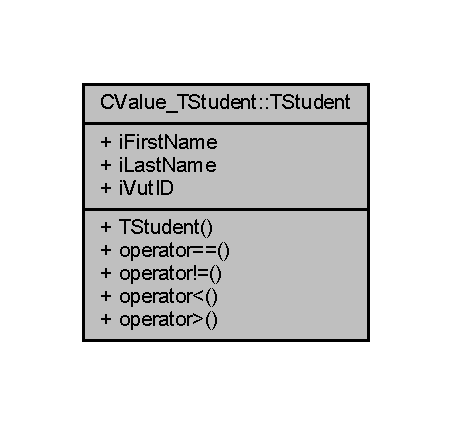
\includegraphics[width=217pt]{struct_c_value___t_student_1_1_t_student__coll__graph}
\end{center}
\end{figure}
\subsection*{Public Member Functions}
\begin{DoxyCompactItemize}
\item 
\hyperlink{struct_c_value___t_student_1_1_t_student_ae052eac687165ae925ca2a15bccc9d95}{T\+Student} (char $\ast$a\+Fisrt\+Name, char $\ast$a\+Last\+Name, int a\+Vut\+ID)
\item 
bool \hyperlink{struct_c_value___t_student_1_1_t_student_ac12071cfbbb72f3666833d7da227f052}{operator==} (const \hyperlink{struct_c_value___t_student_1_1_t_student}{T\+Student} \&a\+Student)
\item 
bool \hyperlink{struct_c_value___t_student_1_1_t_student_aaadc7d5525e434de77c6874052174903}{operator!=} (const \hyperlink{struct_c_value___t_student_1_1_t_student}{T\+Student} \&a\+Student)
\item 
bool \hyperlink{struct_c_value___t_student_1_1_t_student_a0e70d174799ef62209bfd2719077f127}{operator$<$} (const \hyperlink{struct_c_value___t_student_1_1_t_student}{T\+Student} \&a\+Student)
\item 
bool \hyperlink{struct_c_value___t_student_1_1_t_student_ae31809572b52d475b4e891b2a4acaafd}{operator$>$} (const \hyperlink{struct_c_value___t_student_1_1_t_student}{T\+Student} \&a\+Student)
\end{DoxyCompactItemize}
\subsection*{Public Attributes}
\begin{DoxyCompactItemize}
\item 
char $\ast$ \hyperlink{struct_c_value___t_student_1_1_t_student_a5eb1830e69db30e4e2a54d6bdc3f649f}{i\+First\+Name}
\item 
char $\ast$ \hyperlink{struct_c_value___t_student_1_1_t_student_a00b625fc49750e98e28e9d0d013bba66}{i\+Last\+Name}
\item 
int \hyperlink{struct_c_value___t_student_1_1_t_student_aaf7deea3a78dc217d85b4e23f677150f}{i\+Vut\+ID}
\end{DoxyCompactItemize}


\subsection{Detailed Description}
Basic definition of struct type for representing day of week. 

Definition at line 24 of file C\+Value\+\_\+\+T\+Student.\+h.



\subsection{Constructor \& Destructor Documentation}
\mbox{\Hypertarget{struct_c_value___t_student_1_1_t_student_ae052eac687165ae925ca2a15bccc9d95}\label{struct_c_value___t_student_1_1_t_student_ae052eac687165ae925ca2a15bccc9d95}} 
\index{C\+Value\+\_\+\+T\+Student\+::\+T\+Student@{C\+Value\+\_\+\+T\+Student\+::\+T\+Student}!T\+Student@{T\+Student}}
\index{T\+Student@{T\+Student}!C\+Value\+\_\+\+T\+Student\+::\+T\+Student@{C\+Value\+\_\+\+T\+Student\+::\+T\+Student}}
\subsubsection{\texorpdfstring{T\+Student()}{TStudent()}}
{\footnotesize\ttfamily C\+Value\+\_\+\+T\+Student\+::\+T\+Student\+::\+T\+Student (\begin{DoxyParamCaption}\item[{char $\ast$}]{a\+Fisrt\+Name,  }\item[{char $\ast$}]{a\+Last\+Name,  }\item[{int}]{a\+Vut\+ID }\end{DoxyParamCaption})\hspace{0.3cm}{\ttfamily [inline]}}

\begin{DoxyRefDesc}{Bug}
\item[\hyperlink{bug__bug000001}{Bug}]\mbox{[}Zad\mbox{]} Tohle neni dobre, protoze si berete ukazatel na cizi retezec. Lepe je udelat si kopii. \end{DoxyRefDesc}


Definition at line 29 of file C\+Value\+\_\+\+T\+Student.\+h.



\subsection{Member Function Documentation}
\mbox{\Hypertarget{struct_c_value___t_student_1_1_t_student_aaadc7d5525e434de77c6874052174903}\label{struct_c_value___t_student_1_1_t_student_aaadc7d5525e434de77c6874052174903}} 
\index{C\+Value\+\_\+\+T\+Student\+::\+T\+Student@{C\+Value\+\_\+\+T\+Student\+::\+T\+Student}!operator"!=@{operator"!=}}
\index{operator"!=@{operator"!=}!C\+Value\+\_\+\+T\+Student\+::\+T\+Student@{C\+Value\+\_\+\+T\+Student\+::\+T\+Student}}
\subsubsection{\texorpdfstring{operator"!=()}{operator!=()}}
{\footnotesize\ttfamily bool C\+Value\+\_\+\+T\+Student\+::\+T\+Student\+::operator!= (\begin{DoxyParamCaption}\item[{const \hyperlink{struct_c_value___t_student_1_1_t_student}{T\+Student} \&}]{a\+Student }\end{DoxyParamCaption})\hspace{0.3cm}{\ttfamily [inline]}}



Definition at line 39 of file C\+Value\+\_\+\+T\+Student.\+h.

\mbox{\Hypertarget{struct_c_value___t_student_1_1_t_student_a0e70d174799ef62209bfd2719077f127}\label{struct_c_value___t_student_1_1_t_student_a0e70d174799ef62209bfd2719077f127}} 
\index{C\+Value\+\_\+\+T\+Student\+::\+T\+Student@{C\+Value\+\_\+\+T\+Student\+::\+T\+Student}!operator$<$@{operator$<$}}
\index{operator$<$@{operator$<$}!C\+Value\+\_\+\+T\+Student\+::\+T\+Student@{C\+Value\+\_\+\+T\+Student\+::\+T\+Student}}
\subsubsection{\texorpdfstring{operator$<$()}{operator<()}}
{\footnotesize\ttfamily bool C\+Value\+\_\+\+T\+Student\+::\+T\+Student\+::operator$<$ (\begin{DoxyParamCaption}\item[{const \hyperlink{struct_c_value___t_student_1_1_t_student}{T\+Student} \&}]{a\+Student }\end{DoxyParamCaption})\hspace{0.3cm}{\ttfamily [inline]}}



Definition at line 43 of file C\+Value\+\_\+\+T\+Student.\+h.

\mbox{\Hypertarget{struct_c_value___t_student_1_1_t_student_ac12071cfbbb72f3666833d7da227f052}\label{struct_c_value___t_student_1_1_t_student_ac12071cfbbb72f3666833d7da227f052}} 
\index{C\+Value\+\_\+\+T\+Student\+::\+T\+Student@{C\+Value\+\_\+\+T\+Student\+::\+T\+Student}!operator==@{operator==}}
\index{operator==@{operator==}!C\+Value\+\_\+\+T\+Student\+::\+T\+Student@{C\+Value\+\_\+\+T\+Student\+::\+T\+Student}}
\subsubsection{\texorpdfstring{operator==()}{operator==()}}
{\footnotesize\ttfamily bool C\+Value\+\_\+\+T\+Student\+::\+T\+Student\+::operator== (\begin{DoxyParamCaption}\item[{const \hyperlink{struct_c_value___t_student_1_1_t_student}{T\+Student} \&}]{a\+Student }\end{DoxyParamCaption})\hspace{0.3cm}{\ttfamily [inline]}}



Definition at line 35 of file C\+Value\+\_\+\+T\+Student.\+h.

\mbox{\Hypertarget{struct_c_value___t_student_1_1_t_student_ae31809572b52d475b4e891b2a4acaafd}\label{struct_c_value___t_student_1_1_t_student_ae31809572b52d475b4e891b2a4acaafd}} 
\index{C\+Value\+\_\+\+T\+Student\+::\+T\+Student@{C\+Value\+\_\+\+T\+Student\+::\+T\+Student}!operator$>$@{operator$>$}}
\index{operator$>$@{operator$>$}!C\+Value\+\_\+\+T\+Student\+::\+T\+Student@{C\+Value\+\_\+\+T\+Student\+::\+T\+Student}}
\subsubsection{\texorpdfstring{operator$>$()}{operator>()}}
{\footnotesize\ttfamily bool C\+Value\+\_\+\+T\+Student\+::\+T\+Student\+::operator$>$ (\begin{DoxyParamCaption}\item[{const \hyperlink{struct_c_value___t_student_1_1_t_student}{T\+Student} \&}]{a\+Student }\end{DoxyParamCaption})\hspace{0.3cm}{\ttfamily [inline]}}



Definition at line 47 of file C\+Value\+\_\+\+T\+Student.\+h.



\subsection{Member Data Documentation}
\mbox{\Hypertarget{struct_c_value___t_student_1_1_t_student_a5eb1830e69db30e4e2a54d6bdc3f649f}\label{struct_c_value___t_student_1_1_t_student_a5eb1830e69db30e4e2a54d6bdc3f649f}} 
\index{C\+Value\+\_\+\+T\+Student\+::\+T\+Student@{C\+Value\+\_\+\+T\+Student\+::\+T\+Student}!i\+First\+Name@{i\+First\+Name}}
\index{i\+First\+Name@{i\+First\+Name}!C\+Value\+\_\+\+T\+Student\+::\+T\+Student@{C\+Value\+\_\+\+T\+Student\+::\+T\+Student}}
\subsubsection{\texorpdfstring{i\+First\+Name}{iFirstName}}
{\footnotesize\ttfamily char$\ast$ C\+Value\+\_\+\+T\+Student\+::\+T\+Student\+::i\+First\+Name}



Definition at line 25 of file C\+Value\+\_\+\+T\+Student.\+h.

\mbox{\Hypertarget{struct_c_value___t_student_1_1_t_student_a00b625fc49750e98e28e9d0d013bba66}\label{struct_c_value___t_student_1_1_t_student_a00b625fc49750e98e28e9d0d013bba66}} 
\index{C\+Value\+\_\+\+T\+Student\+::\+T\+Student@{C\+Value\+\_\+\+T\+Student\+::\+T\+Student}!i\+Last\+Name@{i\+Last\+Name}}
\index{i\+Last\+Name@{i\+Last\+Name}!C\+Value\+\_\+\+T\+Student\+::\+T\+Student@{C\+Value\+\_\+\+T\+Student\+::\+T\+Student}}
\subsubsection{\texorpdfstring{i\+Last\+Name}{iLastName}}
{\footnotesize\ttfamily char$\ast$ C\+Value\+\_\+\+T\+Student\+::\+T\+Student\+::i\+Last\+Name}



Definition at line 26 of file C\+Value\+\_\+\+T\+Student.\+h.

\mbox{\Hypertarget{struct_c_value___t_student_1_1_t_student_aaf7deea3a78dc217d85b4e23f677150f}\label{struct_c_value___t_student_1_1_t_student_aaf7deea3a78dc217d85b4e23f677150f}} 
\index{C\+Value\+\_\+\+T\+Student\+::\+T\+Student@{C\+Value\+\_\+\+T\+Student\+::\+T\+Student}!i\+Vut\+ID@{i\+Vut\+ID}}
\index{i\+Vut\+ID@{i\+Vut\+ID}!C\+Value\+\_\+\+T\+Student\+::\+T\+Student@{C\+Value\+\_\+\+T\+Student\+::\+T\+Student}}
\subsubsection{\texorpdfstring{i\+Vut\+ID}{iVutID}}
{\footnotesize\ttfamily int C\+Value\+\_\+\+T\+Student\+::\+T\+Student\+::i\+Vut\+ID}



Definition at line 27 of file C\+Value\+\_\+\+T\+Student.\+h.



The documentation for this struct was generated from the following file\+:\begin{DoxyCompactItemize}
\item 
\hyperlink{_c_value___t_student_8h}{C\+Value\+\_\+\+T\+Student.\+h}\end{DoxyCompactItemize}

\chapter{File Documentation}
\hypertarget{_c_hash_map_8cpp}{}\section{C\+Hash\+Map.\+cpp File Reference}
\label{_c_hash_map_8cpp}\index{C\+Hash\+Map.\+cpp@{C\+Hash\+Map.\+cpp}}


\hyperlink{class_c_hash_map}{C\+Hash\+Map} class implementation.  


{\ttfamily \#include \char`\"{}C\+Hash\+Map.\+h\char`\"{}}\newline
Include dependency graph for C\+Hash\+Map.\+cpp\+:
\nopagebreak
\begin{figure}[H]
\begin{center}
\leavevmode
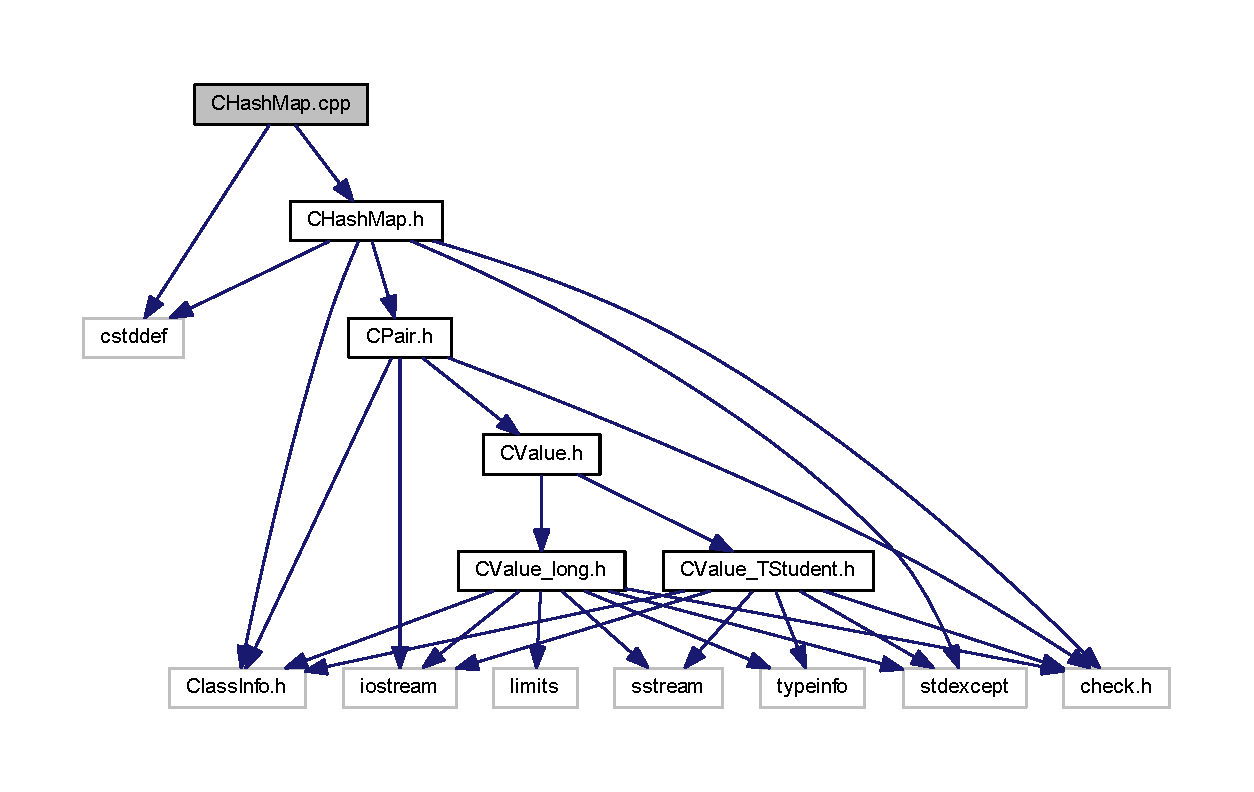
\includegraphics[width=350pt]{_c_hash_map_8cpp__incl}
\end{center}
\end{figure}


\subsection{Detailed Description}
\hyperlink{class_c_hash_map}{C\+Hash\+Map} class implementation. 

File contain \hyperlink{class_c_hash_map}{C\+Hash\+Map} class container implementation. \begin{DoxyAuthor}{Authors}
Pety 2017 
\end{DoxyAuthor}
\begin{DoxyParagraph}{Id}
\hyperlink{_c_hash_map_8cpp}{C\+Hash\+Map.\+cpp} 483 2017-\/11-\/20 16\+:11\+:23Z xlevri01 
\end{DoxyParagraph}

\hypertarget{_c_hash_map_8h}{}\section{C\+Hash\+Map.\+h File Reference}
\label{_c_hash_map_8h}\index{C\+Hash\+Map.\+h@{C\+Hash\+Map.\+h}}


\hyperlink{class_c_hash_map}{C\+Hash\+Map} class header.  


{\ttfamily \#include $<$cstddef$>$}\newline
{\ttfamily \#include $<$stdexcept$>$}\newline
{\ttfamily \#include \char`\"{}C\+Pair.\+h\char`\"{}}\newline
{\ttfamily \#include \char`\"{}Class\+Info.\+h\char`\"{}}\newline
{\ttfamily \#include \char`\"{}check.\+h\char`\"{}}\newline
Include dependency graph for C\+Hash\+Map.\+h\+:\nopagebreak
\begin{figure}[H]
\begin{center}
\leavevmode
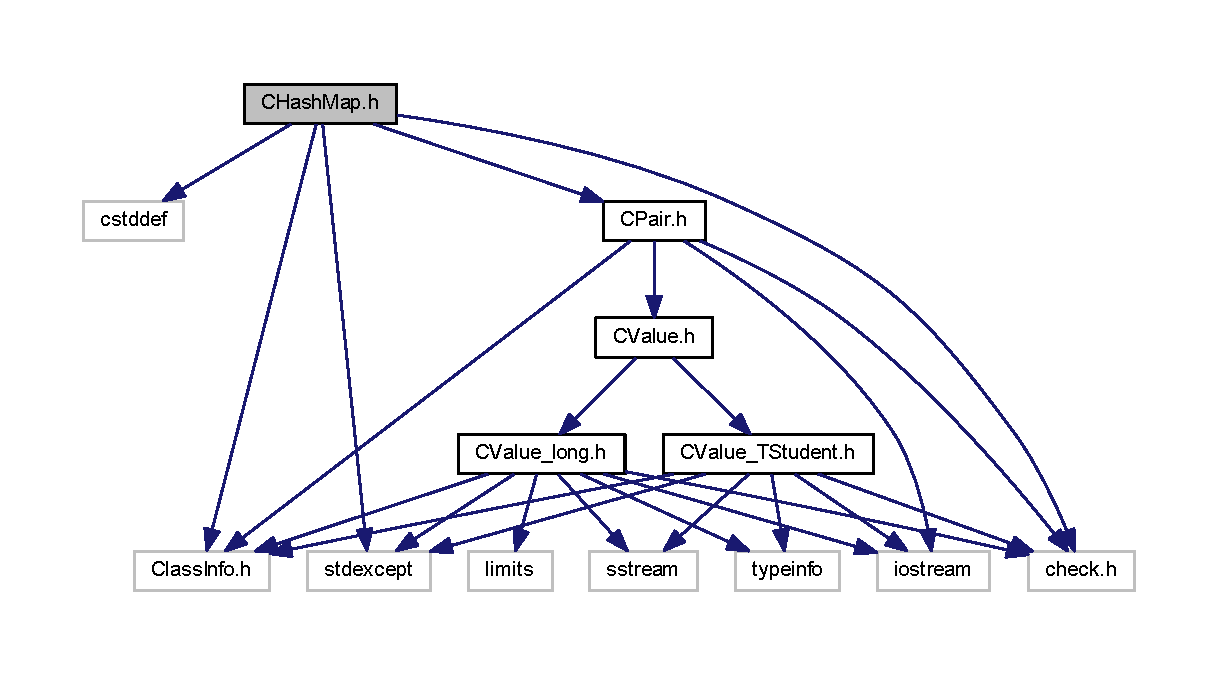
\includegraphics[width=350pt]{_c_hash_map_8h__incl}
\end{center}
\end{figure}
This graph shows which files directly or indirectly include this file\+:\nopagebreak
\begin{figure}[H]
\begin{center}
\leavevmode
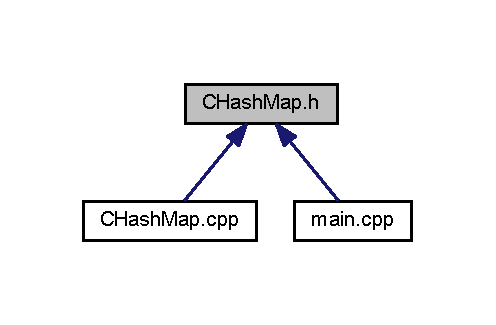
\includegraphics[width=350pt]{_c_hash_map_8h__dep__incl}
\end{center}
\end{figure}
\subsection*{Classes}
\begin{DoxyCompactItemize}
\item 
class \hyperlink{class_c_hash_map}{C\+Hash\+Map}
\begin{DoxyCompactList}\small\item\em \hyperlink{class_c_hash_map}{C\+Hash\+Map} class definition. \end{DoxyCompactList}\item 
struct \hyperlink{struct_c_hash_map_1_1_t_item}{C\+Hash\+Map\+::\+T\+Item}
\begin{DoxyCompactList}\small\item\em \hyperlink{struct_c_hash_map_1_1_t_item}{T\+Item} structure definiton. \end{DoxyCompactList}\item 
struct \hyperlink{struct_c_hash_map_1_1_t_bucket}{C\+Hash\+Map\+::\+T\+Bucket}
\begin{DoxyCompactList}\small\item\em \hyperlink{struct_c_hash_map_1_1_t_bucket}{T\+Bucket} structure definition. \end{DoxyCompactList}\item 
class \hyperlink{class_c_hash_map_1_1_c_forward_iterator}{C\+Hash\+Map\+::\+C\+Forward\+Iterator}
\begin{DoxyCompactList}\small\item\em \hyperlink{class_c_hash_map_1_1_c_forward_iterator}{C\+Forward\+Iterator} class definition. \end{DoxyCompactList}\end{DoxyCompactItemize}


\subsection{Detailed Description}
\hyperlink{class_c_hash_map}{C\+Hash\+Map} class header. 

File contain \hyperlink{class_c_hash_map}{C\+Hash\+Map} class container definition. \begin{DoxyWarning}{Warning}
Don\textquotesingle{}t modify this file 
\end{DoxyWarning}
\begin{DoxyAuthor}{Author}
Pety 2017 
\end{DoxyAuthor}
\begin{DoxyVersion}{Version}

\end{DoxyVersion}
\begin{DoxyParagraph}{Revision}
564 
\end{DoxyParagraph}
\begin{DoxyParagraph}{Id}
\hyperlink{_c_hash_map_8h}{C\+Hash\+Map.\+h} 564 2017-\/11-\/27 09\+:31\+:23Z petyovsky 
\end{DoxyParagraph}

\hypertarget{_c_pair_8cpp}{}\section{C\+Pair.\+cpp File Reference}
\label{_c_pair_8cpp}\index{C\+Pair.\+cpp@{C\+Pair.\+cpp}}


\hyperlink{class_c_pair}{C\+Pair} class implementation.  


{\ttfamily \#include $<$sstream$>$}\newline
{\ttfamily \#include $<$stdexcept$>$}\newline
{\ttfamily \#include \char`\"{}C\+Pair.\+h\char`\"{}}\newline
Include dependency graph for C\+Pair.\+cpp\+:
\nopagebreak
\begin{figure}[H]
\begin{center}
\leavevmode
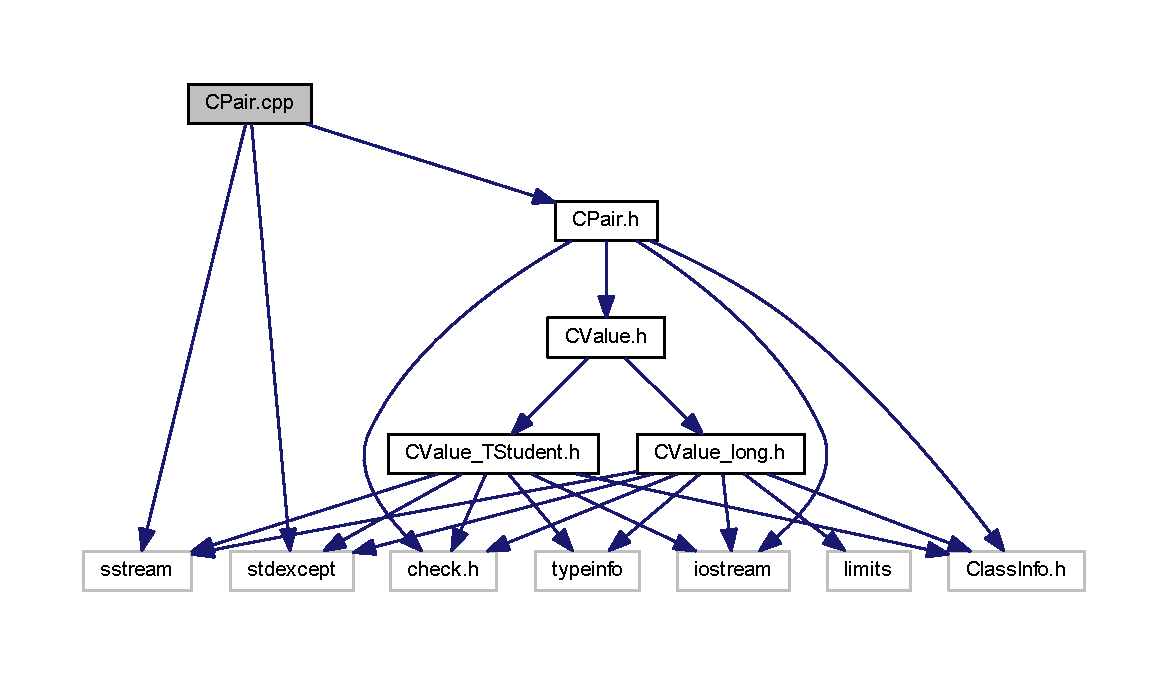
\includegraphics[width=350pt]{_c_pair_8cpp__incl}
\end{center}
\end{figure}


\subsection{Detailed Description}
\hyperlink{class_c_pair}{C\+Pair} class implementation. 

File contain \hyperlink{class_c_pair}{C\+Pair} class (key and value) implementation. \begin{DoxyParagraph}{Id}
\hyperlink{_c_pair_8cpp}{C\+Pair.\+cpp} 129 2017-\/11-\/06 15\+:57\+:56Z xmagat01 
\end{DoxyParagraph}

\hypertarget{_c_pair_8h}{}\section{C\+Pair.\+h File Reference}
\label{_c_pair_8h}\index{C\+Pair.\+h@{C\+Pair.\+h}}


\hyperlink{class_c_pair}{C\+Pair} class header.  


{\ttfamily \#include $<$iostream$>$}\newline
{\ttfamily \#include \char`\"{}C\+Value.\+h\char`\"{}}\newline
{\ttfamily \#include \char`\"{}Class\+Info.\+h\char`\"{}}\newline
{\ttfamily \#include \char`\"{}check.\+h\char`\"{}}\newline
Include dependency graph for C\+Pair.\+h\+:\nopagebreak
\begin{figure}[H]
\begin{center}
\leavevmode
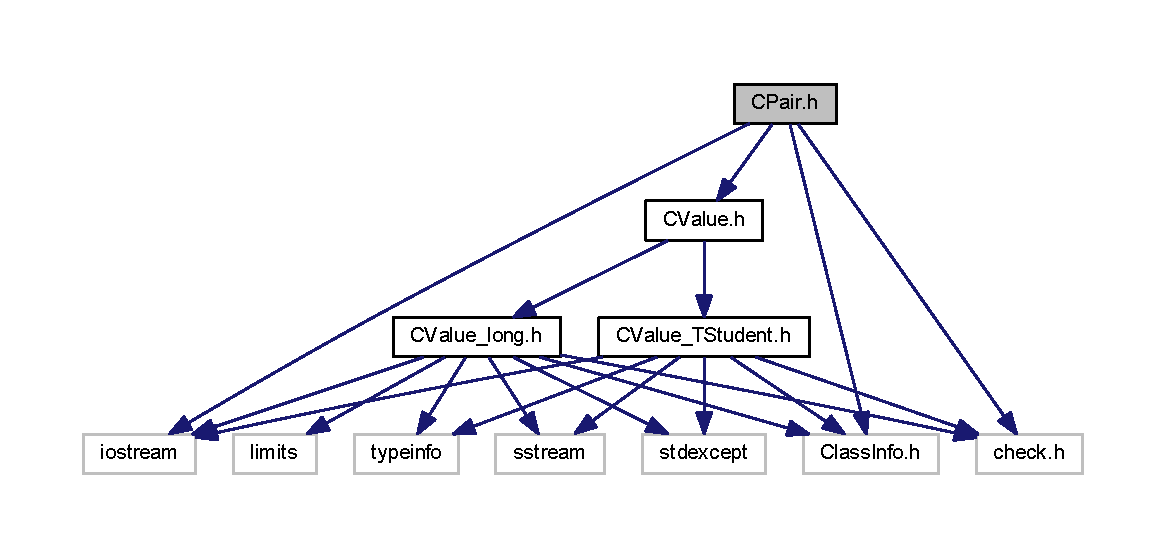
\includegraphics[width=350pt]{_c_pair_8h__incl}
\end{center}
\end{figure}
This graph shows which files directly or indirectly include this file\+:\nopagebreak
\begin{figure}[H]
\begin{center}
\leavevmode
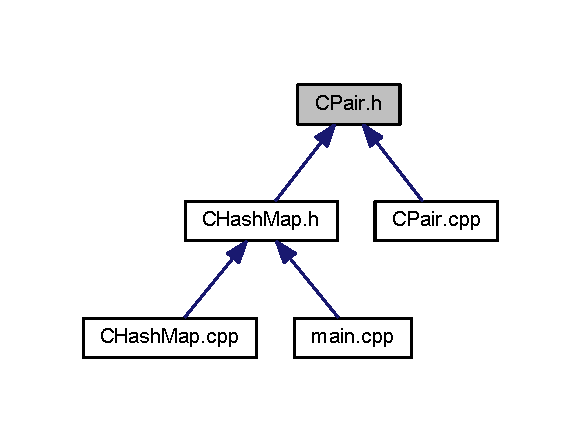
\includegraphics[width=350pt]{_c_pair_8h__dep__incl}
\end{center}
\end{figure}
\subsection*{Classes}
\begin{DoxyCompactItemize}
\item 
class \hyperlink{class_c_pair}{C\+Pair}
\begin{DoxyCompactList}\small\item\em \hyperlink{class_c_pair}{C\+Pair} class (key and value) \end{DoxyCompactList}\end{DoxyCompactItemize}


\subsection{Detailed Description}
\hyperlink{class_c_pair}{C\+Pair} class header. 

File contain \hyperlink{class_c_pair}{C\+Pair} class (key and value) definition. \begin{DoxyWarning}{Warning}
Don\textquotesingle{}t modify this file 
\end{DoxyWarning}
\begin{DoxyAuthor}{Author}
Pety 2017 
\end{DoxyAuthor}
\begin{DoxyVersion}{Version}

\end{DoxyVersion}
\begin{DoxyParagraph}{Revision}
564 
\end{DoxyParagraph}
\begin{DoxyParagraph}{Id}
\hyperlink{_c_pair_8h}{C\+Pair.\+h} 564 2017-\/11-\/27 09\+:31\+:23Z petyovsky 
\end{DoxyParagraph}

\hypertarget{_c_value_8h}{}\section{C\+Value.\+h File Reference}
\label{_c_value_8h}\index{C\+Value.\+h@{C\+Value.\+h}}


General header for C\+Value.  


{\ttfamily \#include \char`\"{}C\+Value\+\_\+long.\+h\char`\"{}}\newline
{\ttfamily \#include \char`\"{}C\+Value\+\_\+\+T\+Student.\+h\char`\"{}}\newline
Include dependency graph for C\+Value.\+h\+:
\nopagebreak
\begin{figure}[H]
\begin{center}
\leavevmode
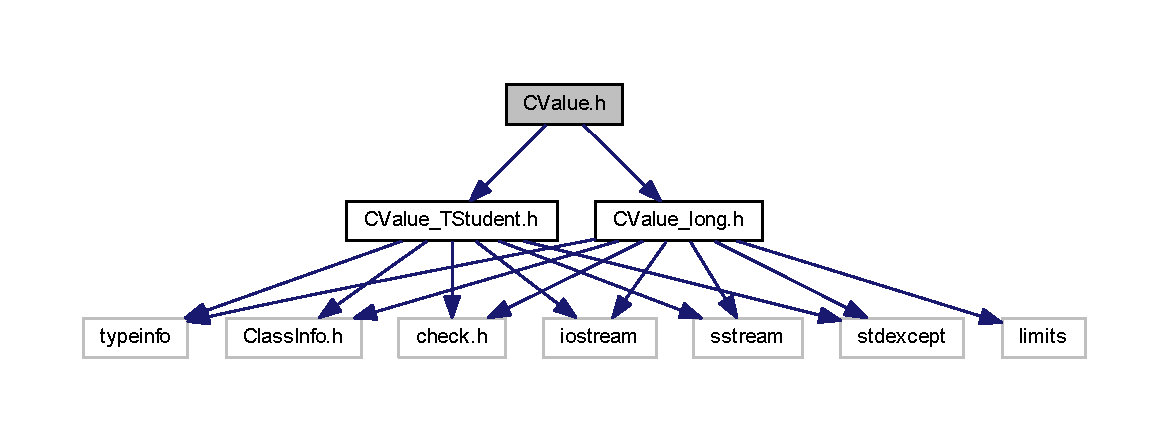
\includegraphics[width=350pt]{_c_value_8h__incl}
\end{center}
\end{figure}
This graph shows which files directly or indirectly include this file\+:
\nopagebreak
\begin{figure}[H]
\begin{center}
\leavevmode
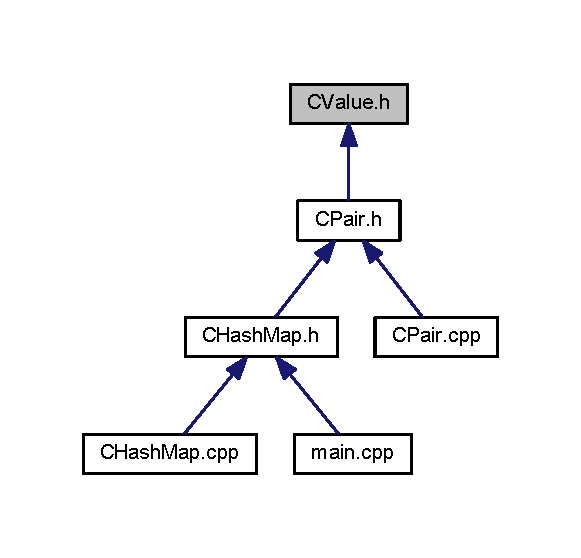
\includegraphics[width=279pt]{_c_value_8h__dep__incl}
\end{center}
\end{figure}
\subsection*{Macros}
\begin{DoxyCompactItemize}
\item 
\#define \hyperlink{_c_value_8h_af4e973b804a5e7cfe45c1aaf5525682d}{C\+V\+A\+L\+U\+E\+\_\+\+T\+E\+S\+T\+\_\+\+A\+PI}
\begin{DoxyCompactList}\small\item\em If defined C\+Value have special A\+P\+Is for testing. \end{DoxyCompactList}\end{DoxyCompactItemize}


\subsection{Detailed Description}
General header for C\+Value. 

Header file for switching C\+Value variant. \begin{DoxyAuthor}{Author}
Pety 2017 
\end{DoxyAuthor}
\begin{DoxyParagraph}{Id}
\hyperlink{_c_value_8h}{C\+Value.\+h} 869 2017-\/12-\/02 21\+:57\+:19Z xmagat01 
\end{DoxyParagraph}


\subsection{Macro Definition Documentation}
\mbox{\Hypertarget{_c_value_8h_af4e973b804a5e7cfe45c1aaf5525682d}\label{_c_value_8h_af4e973b804a5e7cfe45c1aaf5525682d}} 
\index{C\+Value.\+h@{C\+Value.\+h}!C\+V\+A\+L\+U\+E\+\_\+\+T\+E\+S\+T\+\_\+\+A\+PI@{C\+V\+A\+L\+U\+E\+\_\+\+T\+E\+S\+T\+\_\+\+A\+PI}}
\index{C\+V\+A\+L\+U\+E\+\_\+\+T\+E\+S\+T\+\_\+\+A\+PI@{C\+V\+A\+L\+U\+E\+\_\+\+T\+E\+S\+T\+\_\+\+A\+PI}!C\+Value.\+h@{C\+Value.\+h}}
\subsubsection{\texorpdfstring{C\+V\+A\+L\+U\+E\+\_\+\+T\+E\+S\+T\+\_\+\+A\+PI}{CVALUE\_TEST\_API}}
{\footnotesize\ttfamily \#define C\+V\+A\+L\+U\+E\+\_\+\+T\+E\+S\+T\+\_\+\+A\+PI}



If defined C\+Value have special A\+P\+Is for testing. 



Definition at line 11 of file C\+Value.\+h.


\hypertarget{_c_value__bool_8h}{}\section{C\+Value\+\_\+bool.\+h File Reference}
\label{_c_value__bool_8h}\index{C\+Value\+\_\+bool.\+h@{C\+Value\+\_\+bool.\+h}}


\hyperlink{namespace_c_value__bool}{C\+Value\+\_\+bool} class header.  


{\ttfamily \#include $<$iostream$>$}\newline
{\ttfamily \#include $<$sstream$>$}\newline
{\ttfamily \#include $<$stdexcept$>$}\newline
{\ttfamily \#include $<$typeinfo$>$}\newline
{\ttfamily \#include \char`\"{}Class\+Info.\+h\char`\"{}}\newline
{\ttfamily \#include \char`\"{}check.\+h\char`\"{}}\newline
Include dependency graph for C\+Value\+\_\+bool.\+h\+:\nopagebreak
\begin{figure}[H]
\begin{center}
\leavevmode
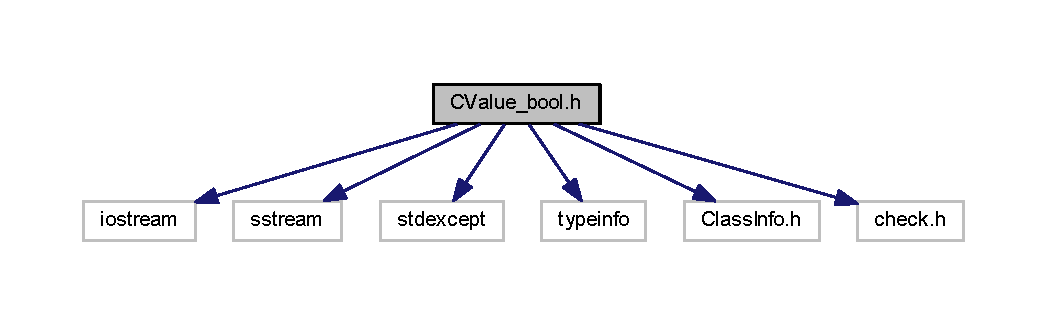
\includegraphics[width=350pt]{_c_value__bool_8h__incl}
\end{center}
\end{figure}
\subsection*{Classes}
\begin{DoxyCompactItemize}
\item 
class \hyperlink{class_c_value__bool_1_1_c_value}{C\+Value\+\_\+bool\+::\+C\+Value}
\begin{DoxyCompactList}\small\item\em \hyperlink{class_c_value__bool_1_1_c_value}{C\+Value} class ({\ttfamily bool} variant) \end{DoxyCompactList}\end{DoxyCompactItemize}
\subsection*{Namespaces}
\begin{DoxyCompactItemize}
\item 
 \hyperlink{namespace_c_value__bool}{C\+Value\+\_\+bool}
\begin{DoxyCompactList}\small\item\em Namespace for encapsulating of {\ttfamily bool} variant of \hyperlink{class_c_value__bool_1_1_c_value}{C\+Value} class. \end{DoxyCompactList}\end{DoxyCompactItemize}


\subsection{Detailed Description}
\hyperlink{namespace_c_value__bool}{C\+Value\+\_\+bool} class header. 

File contain \hyperlink{class_c_value__bool_1_1_c_value}{C\+Value\+\_\+bool\+::\+C\+Value} definition. \begin{DoxyWarning}{Warning}
Don\textquotesingle{}t modify this file 
\end{DoxyWarning}
\begin{DoxyAuthor}{Author}
Pety 2017 
\end{DoxyAuthor}
\begin{DoxyParagraph}{Id}
\hyperlink{_c_value__bool_8h}{C\+Value\+\_\+bool.\+h} 564 2017-\/11-\/27 09\+:31\+:23Z petyovsky 
\end{DoxyParagraph}

\hypertarget{_c_value__long_8h}{}\section{C\+Value\+\_\+long.\+h File Reference}
\label{_c_value__long_8h}\index{C\+Value\+\_\+long.\+h@{C\+Value\+\_\+long.\+h}}


\hyperlink{namespace_c_value__long}{C\+Value\+\_\+long} class header.  


{\ttfamily \#include $<$iostream$>$}\newline
{\ttfamily \#include $<$sstream$>$}\newline
{\ttfamily \#include $<$stdexcept$>$}\newline
{\ttfamily \#include $<$typeinfo$>$}\newline
{\ttfamily \#include $<$limits$>$}\newline
{\ttfamily \#include \char`\"{}Class\+Info.\+h\char`\"{}}\newline
{\ttfamily \#include \char`\"{}check.\+h\char`\"{}}\newline
Include dependency graph for C\+Value\+\_\+long.\+h\+:
\nopagebreak
\begin{figure}[H]
\begin{center}
\leavevmode
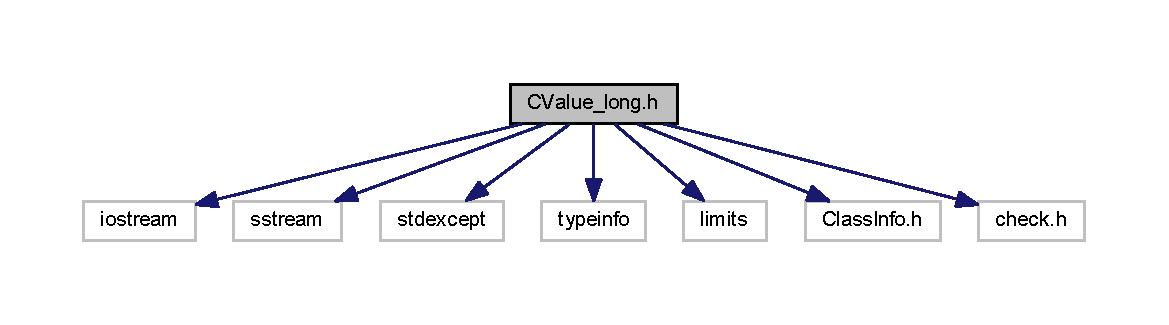
\includegraphics[width=350pt]{_c_value__long_8h__incl}
\end{center}
\end{figure}
This graph shows which files directly or indirectly include this file\+:
\nopagebreak
\begin{figure}[H]
\begin{center}
\leavevmode
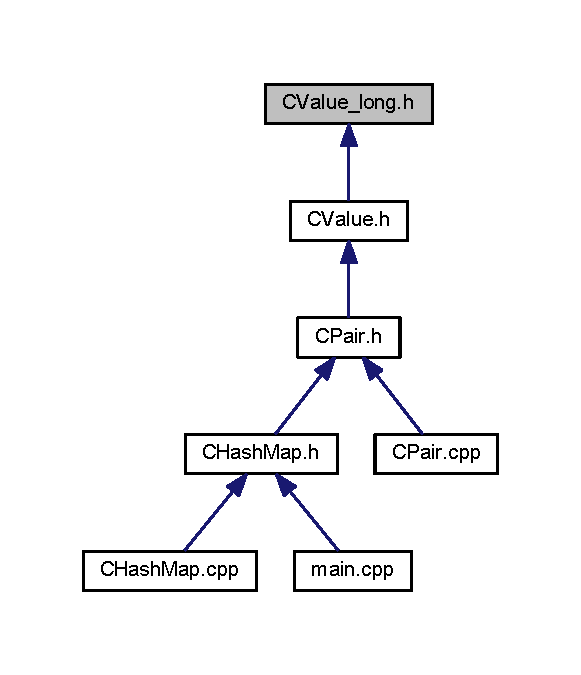
\includegraphics[width=279pt]{_c_value__long_8h__dep__incl}
\end{center}
\end{figure}
\subsection*{Classes}
\begin{DoxyCompactItemize}
\item 
class \hyperlink{class_c_value__long_1_1_c_value}{C\+Value\+\_\+long\+::\+C\+Value}
\begin{DoxyCompactList}\small\item\em \hyperlink{class_c_value__long_1_1_c_value}{C\+Value} class ({\ttfamily long} variant) \end{DoxyCompactList}\end{DoxyCompactItemize}
\subsection*{Namespaces}
\begin{DoxyCompactItemize}
\item 
 \hyperlink{namespace_c_value__long}{C\+Value\+\_\+long}
\begin{DoxyCompactList}\small\item\em Namespace for encapsulating of {\ttfamily long} variant of \hyperlink{class_c_value__long_1_1_c_value}{C\+Value} class. \end{DoxyCompactList}\end{DoxyCompactItemize}


\subsection{Detailed Description}
\hyperlink{namespace_c_value__long}{C\+Value\+\_\+long} class header. 

File contain \hyperlink{class_c_value__long_1_1_c_value}{C\+Value\+\_\+long\+::\+C\+Value} definition. \begin{DoxyWarning}{Warning}
Don\textquotesingle{}t modify this file 
\end{DoxyWarning}
\begin{DoxyAuthor}{Author}
Marek Mag�th 2017 
\end{DoxyAuthor}

\hypertarget{_c_value___t_student_8cpp}{}\section{C\+Value\+\_\+\+T\+Student.\+cpp File Reference}
\label{_c_value___t_student_8cpp}\index{C\+Value\+\_\+\+T\+Student.\+cpp@{C\+Value\+\_\+\+T\+Student.\+cpp}}


\hyperlink{namespace_c_value___t_student}{C\+Value\+\_\+\+T\+Student} class source.  


{\ttfamily \#include \char`\"{}C\+Value\+\_\+\+T\+Student.\+h\char`\"{}}\newline
Include dependency graph for C\+Value\+\_\+\+T\+Student.\+cpp\+:\nopagebreak
\begin{figure}[H]
\begin{center}
\leavevmode
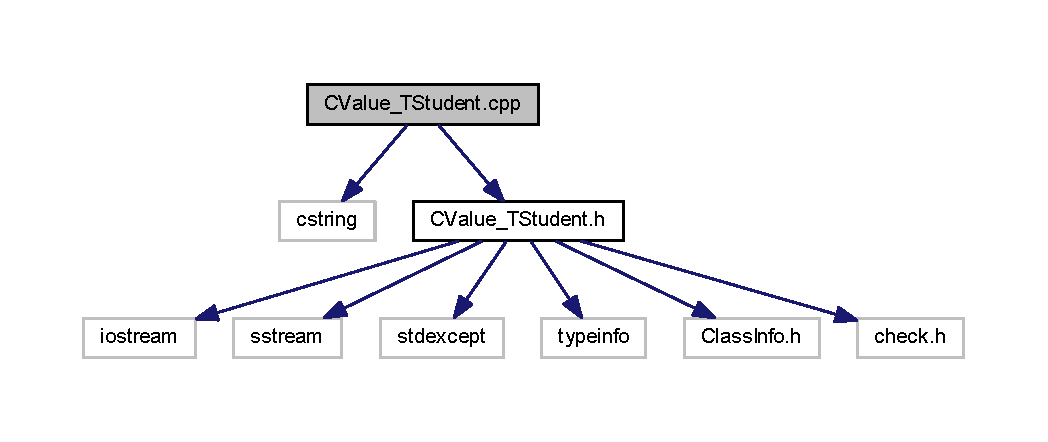
\includegraphics[width=350pt]{_c_value___t_student_8cpp__incl}
\end{center}
\end{figure}
\subsection*{Namespaces}
\begin{DoxyCompactItemize}
\item 
 \hyperlink{namespace_c_value___t_student}{C\+Value\+\_\+\+T\+Student}
\begin{DoxyCompactList}\small\item\em Namespace for encapsulating of {\ttfamily \hyperlink{struct_c_value___t_student_1_1_t_student}{T\+Student}} variant of \hyperlink{class_c_value___t_student_1_1_c_value}{C\+Value} class. \end{DoxyCompactList}\end{DoxyCompactItemize}
\subsection*{Functions}
\begin{DoxyCompactItemize}
\item 
std\+::ostream \& \hyperlink{namespace_c_value___t_student_a74d67e5f2ecbfee96605b87464c628ca}{C\+Value\+\_\+\+T\+Student\+::operator$<$$<$} (std\+::ostream \&a\+O\+Stream, const T\+Student \&a\+Student)
\begin{DoxyCompactList}\small\item\em Output to the stream operator. ({\itshape serialization}) \end{DoxyCompactList}\item 
std\+::istream \& \hyperlink{namespace_c_value___t_student_a7cef4a5db96e988bb59a53168f90363f}{C\+Value\+\_\+\+T\+Student\+::operator$>$$>$} (std\+::istream \&a\+I\+Stream, T\+Student \&a\+Student)
\begin{DoxyCompactList}\small\item\em Input from the stream operator. ({\itshape deserialization}) \end{DoxyCompactList}\end{DoxyCompactItemize}


\subsection{Detailed Description}
\hyperlink{namespace_c_value___t_student}{C\+Value\+\_\+\+T\+Student} class source. 

File contains implementation of \hyperlink{namespace_c_value___t_student}{C\+Value\+\_\+\+T\+Student} global stream operators. \begin{DoxyWarning}{Warning}
Don\textquotesingle{}t modify this file 
\end{DoxyWarning}
\begin{DoxyAuthor}{Author}
Pety 2017 
\end{DoxyAuthor}
\begin{DoxyParagraph}{Id}
\hyperlink{_c_value___t_student_8cpp}{C\+Value\+\_\+\+T\+Student.\+cpp} 1641 2017-\/12-\/10 03\+:35\+:00Z xmagat01 
\end{DoxyParagraph}

\hypertarget{_c_value___t_student_8h}{}\section{C\+Value\+\_\+\+T\+Student.\+h File Reference}
\label{_c_value___t_student_8h}\index{C\+Value\+\_\+\+T\+Student.\+h@{C\+Value\+\_\+\+T\+Student.\+h}}


\hyperlink{namespace_c_value___t_student}{C\+Value\+\_\+\+T\+Student} class header.  


{\ttfamily \#include $<$iostream$>$}\newline
{\ttfamily \#include $<$sstream$>$}\newline
{\ttfamily \#include $<$stdexcept$>$}\newline
{\ttfamily \#include $<$typeinfo$>$}\newline
{\ttfamily \#include \char`\"{}Class\+Info.\+h\char`\"{}}\newline
{\ttfamily \#include \char`\"{}check.\+h\char`\"{}}\newline
Include dependency graph for C\+Value\+\_\+\+T\+Student.\+h\+:\nopagebreak
\begin{figure}[H]
\begin{center}
\leavevmode
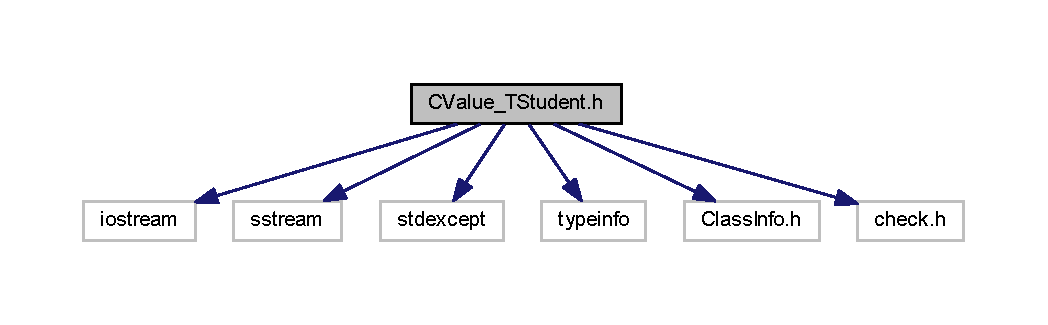
\includegraphics[width=350pt]{_c_value___t_student_8h__incl}
\end{center}
\end{figure}
This graph shows which files directly or indirectly include this file\+:\nopagebreak
\begin{figure}[H]
\begin{center}
\leavevmode
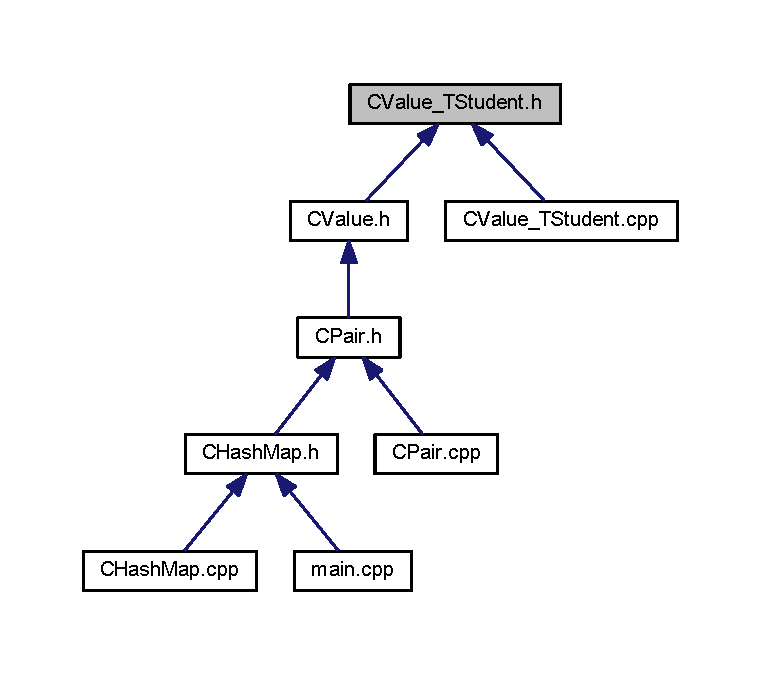
\includegraphics[width=350pt]{_c_value___t_student_8h__dep__incl}
\end{center}
\end{figure}
\subsection*{Classes}
\begin{DoxyCompactItemize}
\item 
struct \hyperlink{struct_c_value___t_student_1_1_t_student}{C\+Value\+\_\+\+T\+Student\+::\+T\+Student}
\begin{DoxyCompactList}\small\item\em Basic definition of struct type for representing \hyperlink{struct_c_value___t_student_1_1_t_student}{T\+Student}. \end{DoxyCompactList}\item 
class \hyperlink{class_c_value___t_student_1_1_c_value}{C\+Value\+\_\+\+T\+Student\+::\+C\+Value}
\begin{DoxyCompactList}\small\item\em \hyperlink{class_c_value___t_student_1_1_c_value}{C\+Value} class ({\ttfamily \hyperlink{struct_c_value___t_student_1_1_t_student}{T\+Student}} variant) \end{DoxyCompactList}\end{DoxyCompactItemize}
\subsection*{Namespaces}
\begin{DoxyCompactItemize}
\item 
 \hyperlink{namespace_c_value___t_student}{C\+Value\+\_\+\+T\+Student}
\begin{DoxyCompactList}\small\item\em Namespace for encapsulating of {\ttfamily \hyperlink{struct_c_value___t_student_1_1_t_student}{T\+Student}} variant of \hyperlink{class_c_value___t_student_1_1_c_value}{C\+Value} class. \end{DoxyCompactList}\end{DoxyCompactItemize}
\subsection*{Functions}
\begin{DoxyCompactItemize}
\item 
std\+::ostream \& \hyperlink{namespace_c_value___t_student_a74d67e5f2ecbfee96605b87464c628ca}{C\+Value\+\_\+\+T\+Student\+::operator$<$$<$} (std\+::ostream \&a\+O\+Stream, const T\+Student \&a\+Student)
\begin{DoxyCompactList}\small\item\em Output to the stream operator. ({\itshape serialization}) \end{DoxyCompactList}\item 
std\+::istream \& \hyperlink{namespace_c_value___t_student_a7cef4a5db96e988bb59a53168f90363f}{C\+Value\+\_\+\+T\+Student\+::operator$>$$>$} (std\+::istream \&a\+I\+Stream, T\+Student \&a\+Student)
\begin{DoxyCompactList}\small\item\em Input from the stream operator. ({\itshape deserialization}) \end{DoxyCompactList}\end{DoxyCompactItemize}


\subsection{Detailed Description}
\hyperlink{namespace_c_value___t_student}{C\+Value\+\_\+\+T\+Student} class header. 

File contain \hyperlink{class_c_value___t_student_1_1_c_value}{C\+Value\+\_\+\+T\+Student\+::\+C\+Value} definition. \begin{DoxyParagraph}{Id}
\hyperlink{_c_value___t_student_8h}{C\+Value\+\_\+\+T\+Student.\+h} 1266 2017-\/12-\/04 23\+:28\+:05Z xmagat01 
\end{DoxyParagraph}

\hypertarget{_c_value___t_week_day_8cpp}{}\section{C\+Value\+\_\+\+T\+Week\+Day.\+cpp File Reference}
\label{_c_value___t_week_day_8cpp}\index{C\+Value\+\_\+\+T\+Week\+Day.\+cpp@{C\+Value\+\_\+\+T\+Week\+Day.\+cpp}}


\hyperlink{namespace_c_value___t_week_day}{C\+Value\+\_\+\+T\+Week\+Day} class source.  


{\ttfamily \#include $<$cstring$>$}\newline
{\ttfamily \#include \char`\"{}C\+Value\+\_\+\+T\+Week\+Day.\+h\char`\"{}}\newline
Include dependency graph for C\+Value\+\_\+\+T\+Week\+Day.\+cpp\+:\nopagebreak
\begin{figure}[H]
\begin{center}
\leavevmode
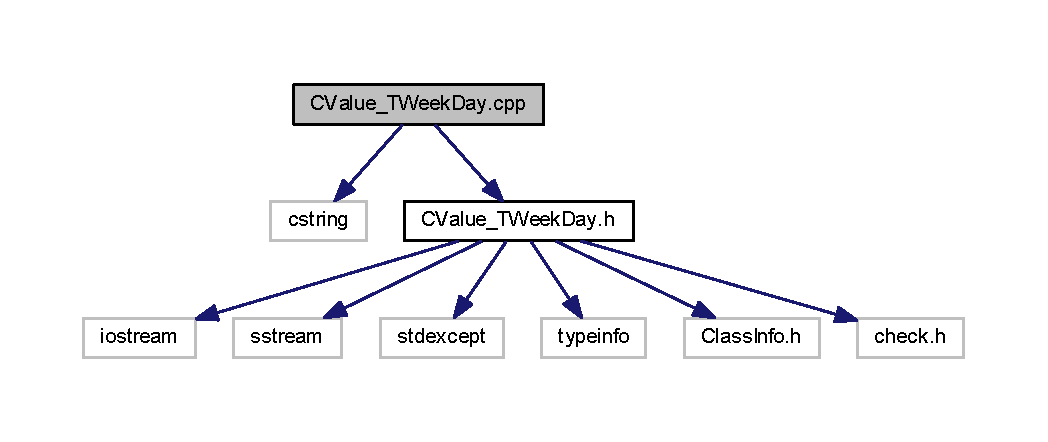
\includegraphics[width=350pt]{_c_value___t_week_day_8cpp__incl}
\end{center}
\end{figure}
\subsection*{Namespaces}
\begin{DoxyCompactItemize}
\item 
 \hyperlink{namespace_c_value___t_week_day}{C\+Value\+\_\+\+T\+Week\+Day}
\begin{DoxyCompactList}\small\item\em Namespace for encapsulating of {\ttfamily T\+Week\+Day} variant of \hyperlink{class_c_value___t_week_day_1_1_c_value}{C\+Value} class. \end{DoxyCompactList}\end{DoxyCompactItemize}
\subsection*{Enumerations}
\begin{DoxyCompactItemize}
\item 
enum \{ \hyperlink{namespace_c_value___t_week_day_ae2f386969b6b243f70cc768d81d87f37a82610dbf312a8592086eff40a38e1ff8}{C\+Value\+\_\+\+T\+Week\+Day\+::\+K\+T\+Week\+Days\+Name\+Max\+Length} = 11
 \}
\end{DoxyCompactItemize}
\subsection*{Functions}
\begin{DoxyCompactItemize}
\item 
T\+Week\+Day \hyperlink{namespace_c_value___t_week_day_ae635bc6aae42ff925b25ce335390083b}{C\+Value\+\_\+\+T\+Week\+Day\+::\+Check\+Range\+With\+Exception} (const unsigned a\+Day\+Num)
\begin{DoxyCompactList}\small\item\em Conversion and range checking function. Convert {\ttfamily unsigned} value to the T\+Week\+Day. \end{DoxyCompactList}\item 
const char $\ast$ \hyperlink{namespace_c_value___t_week_day_ad69753a29bce4084fa5dc888526b2bf2}{C\+Value\+\_\+\+T\+Week\+Day\+::\+T\+Week\+String\+Name} (T\+Week\+Day a\+Week\+Day)
\begin{DoxyCompactList}\small\item\em Conversion Day number to the Day name. \end{DoxyCompactList}\item 
std\+::ostream \& \hyperlink{namespace_c_value___t_week_day_a0783ff307d102432c842a4d943b3d063}{C\+Value\+\_\+\+T\+Week\+Day\+::operator$<$$<$} (std\+::ostream \&a\+O\+Stream, const T\+Week\+Day \&a\+Week\+Day)
\begin{DoxyCompactList}\small\item\em Output to the stream operator. ({\itshape serialization}) \end{DoxyCompactList}\item 
std\+::istream \& \hyperlink{namespace_c_value___t_week_day_ada60106206184e32b42cc05978db4d37}{C\+Value\+\_\+\+T\+Week\+Day\+::operator$>$$>$} (std\+::istream \&a\+I\+Stream, T\+Week\+Day \&a\+Week\+Day)
\begin{DoxyCompactList}\small\item\em Input from the stream operator. ({\itshape deserialization}) \end{DoxyCompactList}\end{DoxyCompactItemize}
\subsection*{Variables}
\begin{DoxyCompactItemize}
\item 
static const char $\ast$const \hyperlink{namespace_c_value___t_week_day_a1c30aa5c20b662fe3dd12e7c26507d27}{C\+Value\+\_\+\+T\+Week\+Day\+::\+K\+T\+Week\+Days\+Name} \mbox{[}K\+T\+Week\+Days\+Count\mbox{]}
\begin{DoxyCompactList}\small\item\em Day name definition. \end{DoxyCompactList}\end{DoxyCompactItemize}


\subsection{Detailed Description}
\hyperlink{namespace_c_value___t_week_day}{C\+Value\+\_\+\+T\+Week\+Day} class source. 

File contains implementation of \hyperlink{namespace_c_value___t_week_day}{C\+Value\+\_\+\+T\+Week\+Day} support functions and global operators also for {\ttfamily enum} T\+Week\+Day \begin{DoxyWarning}{Warning}
Don\textquotesingle{}t modify this file 
\end{DoxyWarning}
\begin{DoxyAuthor}{Author}
Pety 2017 
\end{DoxyAuthor}
\begin{DoxyParagraph}{Id}
\hyperlink{_c_value___t_week_day_8cpp}{C\+Value\+\_\+\+T\+Week\+Day.\+cpp} 564 2017-\/11-\/27 09\+:31\+:23Z petyovsky 
\end{DoxyParagraph}

\hypertarget{_c_value___t_week_day_8h}{}\section{C\+Value\+\_\+\+T\+Week\+Day.\+h File Reference}
\label{_c_value___t_week_day_8h}\index{C\+Value\+\_\+\+T\+Week\+Day.\+h@{C\+Value\+\_\+\+T\+Week\+Day.\+h}}


\hyperlink{namespace_c_value___t_week_day}{C\+Value\+\_\+\+T\+Week\+Day} class header.  


{\ttfamily \#include $<$iostream$>$}\newline
{\ttfamily \#include $<$sstream$>$}\newline
{\ttfamily \#include $<$stdexcept$>$}\newline
{\ttfamily \#include $<$typeinfo$>$}\newline
{\ttfamily \#include \char`\"{}Class\+Info.\+h\char`\"{}}\newline
{\ttfamily \#include \char`\"{}check.\+h\char`\"{}}\newline
Include dependency graph for C\+Value\+\_\+\+T\+Week\+Day.\+h\+:\nopagebreak
\begin{figure}[H]
\begin{center}
\leavevmode
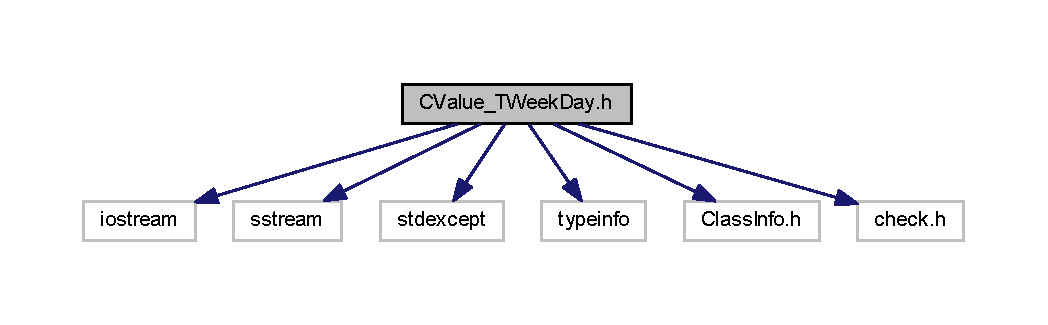
\includegraphics[width=350pt]{_c_value___t_week_day_8h__incl}
\end{center}
\end{figure}
This graph shows which files directly or indirectly include this file\+:\nopagebreak
\begin{figure}[H]
\begin{center}
\leavevmode
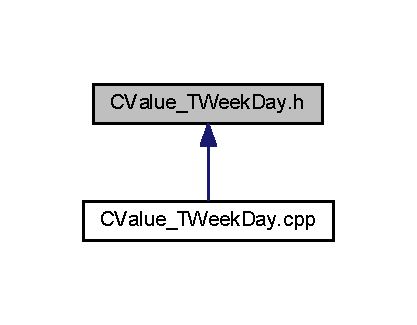
\includegraphics[width=200pt]{_c_value___t_week_day_8h__dep__incl}
\end{center}
\end{figure}
\subsection*{Classes}
\begin{DoxyCompactItemize}
\item 
class \hyperlink{class_c_value___t_week_day_1_1_c_value}{C\+Value\+\_\+\+T\+Week\+Day\+::\+C\+Value}
\begin{DoxyCompactList}\small\item\em \hyperlink{class_c_value___t_week_day_1_1_c_value}{C\+Value} class ({\ttfamily T\+Week\+Day} variant) \end{DoxyCompactList}\end{DoxyCompactItemize}
\subsection*{Namespaces}
\begin{DoxyCompactItemize}
\item 
 \hyperlink{namespace_c_value___t_week_day}{C\+Value\+\_\+\+T\+Week\+Day}
\begin{DoxyCompactList}\small\item\em Namespace for encapsulating of {\ttfamily T\+Week\+Day} variant of \hyperlink{class_c_value___t_week_day_1_1_c_value}{C\+Value} class. \end{DoxyCompactList}\end{DoxyCompactItemize}
\subsection*{Enumerations}
\begin{DoxyCompactItemize}
\item 
enum \hyperlink{namespace_c_value___t_week_day_a6412f204509f223b789fb5f1a61a6124}{C\+Value\+\_\+\+T\+Week\+Day\+::\+T\+Week\+Day} \{ \newline
\hyperlink{namespace_c_value___t_week_day_a6412f204509f223b789fb5f1a61a6124a13c1447b2f5be5b292b403d71b5460b9}{C\+Value\+\_\+\+T\+Week\+Day\+::\+E\+Monday} = 0, 
\hyperlink{namespace_c_value___t_week_day_a6412f204509f223b789fb5f1a61a6124ac54a40e76745b36a2315ffed4edbce80}{C\+Value\+\_\+\+T\+Week\+Day\+::\+E\+Tuesday}, 
\hyperlink{namespace_c_value___t_week_day_a6412f204509f223b789fb5f1a61a6124ac611066963726ce53657cedaaaefc3d5}{C\+Value\+\_\+\+T\+Week\+Day\+::\+E\+Wednesday}, 
\hyperlink{namespace_c_value___t_week_day_a6412f204509f223b789fb5f1a61a6124a7fb51985580d1ba92e55f2577a04b3b1}{C\+Value\+\_\+\+T\+Week\+Day\+::\+E\+Thursday}, 
\newline
\hyperlink{namespace_c_value___t_week_day_a6412f204509f223b789fb5f1a61a6124a5d2ecb8bb6c29d8ecbfc5901ab383978}{C\+Value\+\_\+\+T\+Week\+Day\+::\+E\+Friday}, 
\hyperlink{namespace_c_value___t_week_day_a6412f204509f223b789fb5f1a61a6124ab3e8b0a563537c9cd6ef20d06b486100}{C\+Value\+\_\+\+T\+Week\+Day\+::\+E\+Saturday}, 
\hyperlink{namespace_c_value___t_week_day_a6412f204509f223b789fb5f1a61a6124ad4ed77e2d38772a8a5f77e9f87621117}{C\+Value\+\_\+\+T\+Week\+Day\+::\+E\+Sunday}
 \}\begin{DoxyCompactList}\small\item\em Basic definition of enumeration type for representing day of week. \end{DoxyCompactList}
\item 
enum \{ \hyperlink{namespace_c_value___t_week_day_aafc13db7f1761bc02fc24499d9d30ef8aa662532b91895c243892c79eaafea534}{C\+Value\+\_\+\+T\+Week\+Day\+::\+K\+T\+Week\+Days\+Count} = 7
 \}\begin{DoxyCompactList}\small\item\em Constant defining numbers of day in the week. \end{DoxyCompactList}
\end{DoxyCompactItemize}
\subsection*{Functions}
\begin{DoxyCompactItemize}
\item 
T\+Week\+Day \hyperlink{namespace_c_value___t_week_day_ae635bc6aae42ff925b25ce335390083b}{C\+Value\+\_\+\+T\+Week\+Day\+::\+Check\+Range\+With\+Exception} (const unsigned a\+Day\+Num)
\begin{DoxyCompactList}\small\item\em Conversion and range checking function. Convert {\ttfamily unsigned} value to the T\+Week\+Day. \end{DoxyCompactList}\item 
const char $\ast$ \hyperlink{namespace_c_value___t_week_day_ad69753a29bce4084fa5dc888526b2bf2}{C\+Value\+\_\+\+T\+Week\+Day\+::\+T\+Week\+String\+Name} (T\+Week\+Day a\+Week\+Day)
\begin{DoxyCompactList}\small\item\em Conversion Day number to the Day name. \end{DoxyCompactList}\item 
std\+::ostream \& \hyperlink{namespace_c_value___t_week_day_a0783ff307d102432c842a4d943b3d063}{C\+Value\+\_\+\+T\+Week\+Day\+::operator$<$$<$} (std\+::ostream \&a\+O\+Stream, const T\+Week\+Day \&a\+Week\+Day)
\begin{DoxyCompactList}\small\item\em Output to the stream operator. ({\itshape serialization}) \end{DoxyCompactList}\item 
std\+::istream \& \hyperlink{namespace_c_value___t_week_day_ada60106206184e32b42cc05978db4d37}{C\+Value\+\_\+\+T\+Week\+Day\+::operator$>$$>$} (std\+::istream \&a\+I\+Stream, T\+Week\+Day \&a\+Week\+Day)
\begin{DoxyCompactList}\small\item\em Input from the stream operator. ({\itshape deserialization}) \end{DoxyCompactList}\end{DoxyCompactItemize}


\subsection{Detailed Description}
\hyperlink{namespace_c_value___t_week_day}{C\+Value\+\_\+\+T\+Week\+Day} class header. 

File contain \hyperlink{class_c_value___t_week_day_1_1_c_value}{C\+Value\+\_\+\+T\+Week\+Day\+::\+C\+Value} definition. \begin{DoxyWarning}{Warning}
Don\textquotesingle{}t modify this file 
\end{DoxyWarning}
\begin{DoxyAuthor}{Author}
Pety 2017 
\end{DoxyAuthor}
\begin{DoxyParagraph}{Id}
\hyperlink{_c_value___t_week_day_8h}{C\+Value\+\_\+\+T\+Week\+Day.\+h} 564 2017-\/11-\/27 09\+:31\+:23Z petyovsky 
\end{DoxyParagraph}

\hypertarget{_documentation_8md}{}\section{Documentation.\+md File Reference}
\label{_documentation_8md}\index{Documentation.\+md@{Documentation.\+md}}

\hypertarget{_introduction_8md}{}\section{Introduction.\+md File Reference}
\label{_introduction_8md}\index{Introduction.\+md@{Introduction.\+md}}

\hypertarget{main_8cpp}{}\section{main.\+cpp File Reference}
\label{main_8cpp}\index{main.\+cpp@{main.\+cpp}}
{\ttfamily \#include $<$iostream$>$}\newline
{\ttfamily \#include \char`\"{}C\+Hash\+Map.\+h\char`\"{}}\newline
Include dependency graph for main.\+cpp\+:
\nopagebreak
\begin{figure}[H]
\begin{center}
\leavevmode
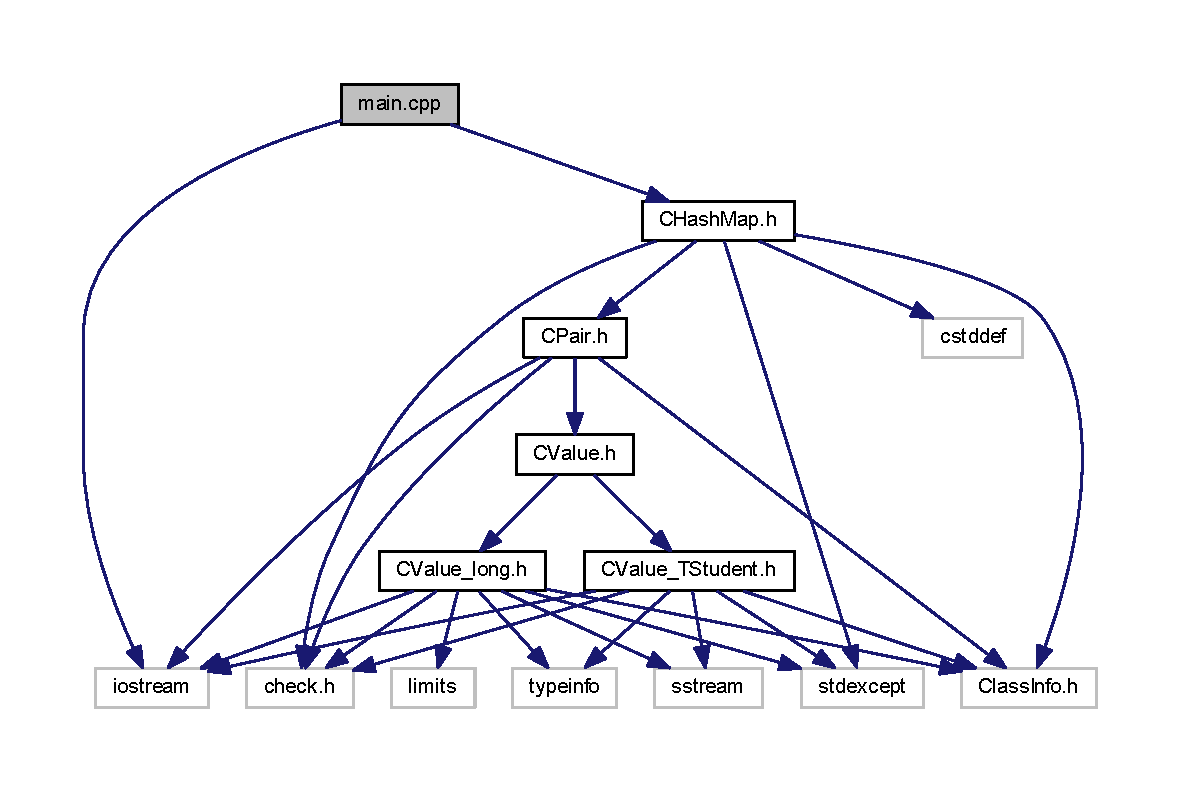
\includegraphics[width=350pt]{main_8cpp__incl}
\end{center}
\end{figure}
\subsection*{Functions}
\begin{DoxyCompactItemize}
\item 
int \hyperlink{main_8cpp_ae66f6b31b5ad750f1fe042a706a4e3d4}{main} ()
\end{DoxyCompactItemize}


\subsection{Function Documentation}
\mbox{\Hypertarget{main_8cpp_ae66f6b31b5ad750f1fe042a706a4e3d4}\label{main_8cpp_ae66f6b31b5ad750f1fe042a706a4e3d4}} 
\index{main.\+cpp@{main.\+cpp}!main@{main}}
\index{main@{main}!main.\+cpp@{main.\+cpp}}
\subsubsection{\texorpdfstring{main()}{main()}}
{\footnotesize\ttfamily int main (\begin{DoxyParamCaption}{ }\end{DoxyParamCaption})}



Definition at line 14 of file main.\+cpp.


%--- End generated contents ---

% Index
\backmatter
\newpage
\phantomsection
\clearemptydoublepage
\addcontentsline{toc}{chapter}{Index}
\printindex

\end{document}
